% This template is mainly taken from Fredrick Font, which I guess to a large extent comes from Joan Serrà. There are some changes to it, mainly taken from Ajay Srinivasamurthy

% What version of the document are you compiling
%\def\DRAFTMODE{}   % Uncomment if generating the draft version
%\def\PRINTVER{}    % Uncomment if generating the final BOOK (print) version (The differences are in 1) Colors of hyperlinks, 2) Bleeds, 3) Trim marks + Size)
% If both the commands are comments it generates a final PDF version to be distributted electronically.

%% Useful packages
\RequirePackage{fix-cm} % Technicalities
% -------------------------------------------------------------------------------------------------------------------------
%\documentclass[11pt,a4paper,twoside,openright]{memoir}	% Some extra options if needed in the future\textsl{}
%\documentclass[10pt,b5paper,twoside,showtrims,openright]{memoir} % Some extra options if needed in the future
%\documentclass[10pt,a4paper,twoside,showtrims,openright]{memoir} % Some extra options if needed in the future
\documentclass[11pt,a4paper,twoside,openright, showtrims, oldfontcommands]{memoir} 

%Fixing imp useful info
\renewcommand{\title}{Computational Approaches for the Melodic Description in Indian Art Music Corpora}
\renewcommand{\author}{Sankalp Gulati}
\newcommand{\thyear}{2016}
\newcommand{\departmenta}{Music Technology Group}
\newcommand{\departmentb}{Dept. of Information and Communication Technologies}
\newcommand{\supervisor}{Dr. Xavier Serra Casals}
% -------------------------------------------------------------------------------------------------------------------------
\usepackage{times}
\usepackage[T1]{fontenc} 
\usepackage[utf8]{inputenc}
\usepackage{mathptmx}
\DeclareMathAlphabet{\mathcal}{OMS}{cmsy}{m}{n}
\DeclareMathAlphabet\mathbfcal{OMS}{cmsy}{b}{n}
%\usepackage{ae,aecompl}
\usepackage[UKenglish]{isodate}

\usepackage[british]{babel}
\usepackage{url}
\urlstyle{rm}
\usepackage{enumitem}
\usepackage{amssymb,amsmath}
\usepackage[pdftex]{graphicx}
\usepackage{epsfig}
\usepackage{lscape} 
\usepackage{color}
\usepackage[table]{xcolor}% for alternating colors in tabels to improve readability
\usepackage{nicefrac}
\usepackage{titlecaps}
\Addlcwords{for, is, on}
\usepackage{titlesec}
\usepackage[round,authoryear]{natbib}
\usepackage{acronym}
%\usepackage[style=long,nonumberlist,toc,acronym,nomain]{glossaries}
\usepackage[section,numberedsection=autolabel,acronym,nonumberlist,nomain,nogroupskip=true]{glossaries}
\usepackage{mathtools}
%\usepackage{longtable}
\usepackage{rotating}
\usepackage{arydshln}
\usepackage{algorithm,algorithmicx}
\usepackage[noend]{algpseudocode}
\usepackage[threshold=0]{csquotes}
\usepackage[pdftex,backref=page,hyperfigures,breaklinks,colorlinks,bookmarksopenlevel=0,bookmarksdepth=2
  pdfpagemode=UseOutlines,
  pdftitle=Computational~Approaches~for~Analysis~and~Description~of~Melodies~in~Indian~Art~Music
  pdfauthor=Sankalp~Gulati,
  pdfsubject=PhD~Thesis,
  pdfkeywords=Melody~Motifs~Patterns~Raga~Phrases~Indian~art~music~Hindustani~Carnatic~MIR~Information~Retrieval
]{hyperref}
\usepackage{listings}
\usepackage[font=small,labelfont=bf]{caption}
\usepackage{subcaption}
%
%\let\footruleskip\undefined
%\usepackage{fancyhdr}
%\pagestyle{fancy}

\setlength{\epigraphwidth}{0.586\textwidth}
\renewcommand{\textflush}{flushleftright}

%\usepackage{natbibspacing}
%\setlength{\bibspacing}{0.3\baselineskip}
% per les pagines a la bibliografia
% -> UN COMMENT A PARTIR D?AQUI
%\renewcommand*{\backref}[1]{}
%\renewcommand*{\backrefalt}[4]{%
%    \ifcase #1 (Not cited.)%
%    \or        (Cited on page~#2.)%
%    \else      (Cited on pages~#2.)%
%    \fi}

\usepackage{fixltx2e} % Technicalities
\usepackage{latexsym}
\usepackage{rotating}
\usepackage{bm}
%\usepackage{bibentry}\nobibliography*
\usepackage{longtable}
%\usepackage{verbatim}
\newsubfloat{figure}
\usepackage{wrapfig}
% better tables
\usepackage[para]{threeparttable}
\usepackage{booktabs}
\usepackage{arydshln}

\newcommand{\ra}[1]{\renewcommand{\arraystretch}{#1}}
\usepackage{array}
\newcolumntype{P}[1]{>{\raggedright\arraybackslash}p{#1}}
\newcolumntype{L}[1]{>{\centering\arraybackslash}m{#1}}
\newcolumntype{T}[1]{>{\raggedleft\arraybackslash}p{#1}}

% for footnotes in tables
\usepackage{footnote}
\usepackage{multirow}
\makesavenoteenv{tabular}
\makesavenoteenv{table}
\usepackage{courier}

\usepackage{ifthen}

\usepackage{chngcntr}
\counterwithout{footnote}{chapter}

\usepackage{lipsum}
\newcommand{\signat}[1]{%
	{%
		\unskip
		\nobreak
		\hfil
		\penalty50%
		\hskip2em%
		\hbox{}%
		\nobreak
		\hfil
		#1%
		\parfillskip=0pt%
		\finalhyphendemerits=0% 
		\endgraf
	}%
}



\maxsecnumdepth{subsubsection}
\setsecnumdepth{subsubsection}
%\maxtocdepth{subsubsection}
%\settocdepth{subsubsection}
\maxtocdepth{subsection}
\settocdepth{subsection}

\definecolor{NoColor}{rgb}{0,0,0}
%%%%%%%%\definecolor{LinkColor}{rgb}{0,0,0.25}
%%%%%%%%\definecolor{ExtLinkColor}{rgb}{0,0.3,0}
\definecolor{tabgray}{gray}{0.8}
\definecolor{CiteColor}{rgb}{0, 0, 0.3} 
\definecolor{LinkColor}{rgb}{0, 0, 0.3} 
% \definecolor{LinkColor}{rgb}{0, 1, 0} 
% \definecolor{ExtLinkColor}{rgb}{0, 0.4, 0}
\definecolor{ExtLinkColor}{rgb}{0, 0, 0.6}

\ifdefined\PRINTVER
\hypersetup{citecolor=black,linkcolor=black,urlcolor=black}
\else
\hypersetup{citecolor=CiteColor,linkcolor=LinkColor,urlcolor=ExtLinkColor}
\fi

%% Format UPF, dues cares. Recordeu que les dimensions d'A4 i B5 son (210mm,297mm) i (176mm,250mm), respectivament.
\setstocksize{297mm}{210mm} % El suport original es A4
\settrimmedsize{250mm}{176mm}{*} % El suport final, despres de tallar, B5.
\setlength{\trimtop}{23mm} % Alcada de la franja superior a tallar.
\setlength{\trimtop}{24mm} % Alcada de la franja inferior a tallar.
\setlength{\trimedge}{17mm} % Amplada de la franja interior a tallar per cada costat.
%\setulmarginsandblock{*}{29mm}{1.1} % Marges verticals (3cm a dalt, 0.9*3cm a baix)
%\setlrmarginsandblock{30mm}{*}{0.75} % Marges laterals (3cm a la dreta, 0.75*3cm l'esquerra)
\setulmarginsandblock{23mm}{23mm}{*} % used to be {25mm}{16mm}
\setlrmarginsandblock{25mm}{*}{0.8}
\checkandfixthelayout
\trimLmarks % Marques de tall en forma de 'L'

%%%%%%%%% TAKEN FROM AJAY SEE IF THIS SIZE LOOKS BETTER OTHERWISE STICK TO WHAT IT IS 
%\ifdefined\PRINTVER
%\setstocksize{297mm}{210mm}  % The size of the stock paper (support), A4
%\settrimmedsize{250mm}{176mm}{*} % B5, the size of the final copy, cut from the stock paper.
%\setlength{\trimtop}{23mm}   % Top margin: top_stock - top_page
%\setlength{\trimedge}{17mm}  % Outer later margin: lat_stock - lat_page
%\setlrmarginsandblock{34mm}{30mm}{*} % 
%\setulmarginsandblock{27mm}{25mm}{*} % 
%\trimLmarks % Ls, not crosses (which may leave traces on the final copy) as trimmarks.
%\checkandfixthelayout
%\else
%\setstocksize{250mm}{176mm}  % The size of the stock paper (support), A4
%\settrimmedsize{\stockheight}{\stockwidth}{*} % B5, the size of the final copy, cut from the stock paper.
%\setlength{\trimtop}{0mm}   % Top margin: top_stock - top_page
%\setlength{\trimedge}{0mm}  % Outer later margin: lat_stock - lat_page
%\setlrmarginsandblock{32mm}{32mm}{*} % 
%\setulmarginsandblock{27mm}{25mm}{1.0} % 
%\showtrimsoff
%\checkandfixthelayout
%\fi

% arreglar que floats al final de capitol no es centrin verticalment
%\makeatletter% Set distance from top of page to first float
%\setlength{\@fptop}{5pt}
%\makeatother

% perque no es posi espai blanc raro entre coses
%\raggedbottom
\flushbottom

% espai despres de floats
\setlength{\textfloatsep}{0.5cm}


% Estil de quan poso tags al text tags
\newcommand{\atag}[1]{\small{\texttt{#1}}\normalsize}

%\makechapterstyle{myveelo}{
%  \setlength{\afterchapskip}{40pt}
%  \renewcommand*{\chapterheadstart}{\vspace*{40pt}}
%  \renewcommand*{\afterchapternum}{\par\nobreak\vskip 25pt}
%  \renewcommand*{\chapnamefont}{\normalfont\LARGE\flushright}
%  \renewcommand*{\chapnumfont}{\normalfont\HUGE}
%  \renewcommand*{\chaptitlefont}{\normalfont\HUGE\bfseries\flushright}
%  \renewcommand*{\printchaptername}{\chapnamefont CHAPTER} %\renewcommand*{\printchaptername}{\chapnamefont\MakeUppercase{\@chapapp}}
%  \renewcommand*{\chapternamenum}{}
%  \setlength{\beforechapskip}{18mm}
%  \setlength{\midchapskip}{\paperwidth}
%  \addtolength{\midchapskip}{-\textwidth}
%  \addtolength{\midchapskip}{-\spinemargin}
%  \renewcommand*{\printchapternum}{
%    \makebox[0pt][l]{
%      \hspace{.8em}
%      \resizebox{!}{1cm}{\chapnumfont \thechapter} %\resizebox{!}{\numberheight}{\chapnumfont \thechapter}
%      \hspace{.8em}
%      \rule{\midchapskip}{\beforechapskip}
%    }
%  }
%  \makeoddfoot{plain}{}{}{\thepage}
%}

\makechapterstyle{myveelo}{
  \renewcommand*{\chapterheadstart}{\vspace*{0.7cm}}
  \renewcommand*{\chapnamefont}{\normalfont\Large}
  \renewcommand*{\chapnumfont}{\normalfont\HUGE}
  \renewcommand*{\chaptitlefont}{\vspace*{-2.1cm}\normalfont\HUGE\bfseries\flushright}
  \renewcommand*{\printchaptername}{\flushright \chapnamefont CHAPTER\ \ \ \ \ \ \ \ }
  \setlength{\beforechapskip}{12mm}
  \setlength{\midchapskip}{\paperwidth}
  \addtolength{\midchapskip}{-\textwidth}
  \addtolength{\midchapskip}{-\spinemargin}
  \setlength{\afterchapskip}{2cm}
  \renewcommand*{\printchapternum}{
    \makebox[0pt][l]{
      \hspace{-1cm}
      \resizebox{!}{1cm}{\chapnumfont \thechapter}
      \hspace{0.4cm}
      \rule{\midchapskip}{\beforechapskip}
    }
  }
  \makeoddfoot{plain}{}{}{\thepage}
}


\makeatletter
\makepagestyle{mainmatter}
\setlength{\headwidth}{\textwidth}
\makerunningwidth{mainmatter}{\headwidth}
\makeheadrule{mainmatter}{\headwidth}{0pt}
\makeheadposition{mainmatter}{flushright}{flushleft}{}{}
\makepsmarks{mainmatter}{%
	\let\@mkboth\markboth
	\def\chaptermark##1{\markboth{##1}{##1}}    % left mark & right marks
	\def\sectionmark##1{\markright{%
			\ifnum \c@secnumdepth>\z@
			\thesection \ \ %
			\fi
			##1}}
	\def\tocmark{\markboth{\contentsname}{\contentsname}}%
	\def\lofmark{\markboth{\listfigurename}{\listfigurename}}%
	\def\lotmark{\markboth{\listtablename}{\listtablename}}%
	\def\bibmark{\markboth{\bibname}{\bibname}}%
	\def\indexmark{\markboth{\indexname}{\indexname}}%
}
\makeevenhead{mainmatter}{\normalfont\thepage}{}%\bfseries
{\normalfont\scshape\leftmark}
\makeoddhead{mainmatter}{\normalfont\scshape\rightmark}{}%
{\normalfont\thepage}%\bfseries
\ifdraftdoc
\makeevenfoot{mainmatter}{\thepage}{}{\textit{Draft: \today, \printtime*{}}}
\makeoddfoot{mainmatter}{\textit{Draft: \today, \printtime*{}}}{}{\thepage}
\fi
\makeatother
% For front matter
\makepagestyle{frontmatter}
\makeevenhead{frontmatter}{\normalfont\thepage}{}{}%\bfseries
\makeoddhead{frontmatter}{}{}{\normalfont\thepage}%\bfseries


%\usepackage{calc}\usepackage{tikz}
%\makechapterstyle{mycombined}{
%  \setlength{\beforechapskip}{1cm}
%  \setlength{\midchapskip}{-80pt}
%  \setlength{\afterchapskip}{2cm}
%  \renewcommand*{\printchaptername}{}
%  \renewcommand*{\chapnumfont}{\normalfont\bfseries\fontsize{60}{0}\selectfont}
%  \renewcommand*{\printchapternum}{
%    %\flushright\chapnumfont\thechapter
%    \flushright 
%    %\normalfont\large\bfseries Chapter
%    \begin{tikzpicture}
%      \draw[fill,color=black] (0,0) rectangle (2cm,2cm);
%      \draw[color=white] (1cm,1cm) node { \chapnumfont\thechapter };
%    \end{tikzpicture}
%    \marginpar{}
%  }
%  \renewcommand*{\chaptitlefont}{\normalfont\HUGE\bfseries}
%  \renewcommand*{\printchaptertitle}[1]{%
%    \raggedright\chaptitlefont\parbox[t]{\textwidth-3cm}{\raggedright##1}}
%}

\chapterstyle{myveelo}
\pagestyle{mainmatter}

% ---- Some configs...



%\renewcommand{\rmdefault}{put}
%\renewcommand{\sfdefault}{phv}
\newcommand{\superscript}[1]{\ensuremath{^{\textrm{#1}}}}
\newcommand{\subscript}[1]{\ensuremath{_{\textrm{#1}}}}
\newcommand{\quotat}[2]{
  \begin{flushright}
    \textit{``#1'',\\
    \vspace*{0.3cm}
    #2.\\
    \vspace*{0.3cm}
    }
  \end{flushright}
}


\renewcommand{\mkcitation}[1]{ (#1)}
%\renewcommand{\mktextquote}[6]{#1#2#3#6#4#5}
%\renewcommand{\mktextquote}[6]{#1#2#4#3\hfill\hbox{#6}#5}
\renewcommand{\mktextquote}[6]{#1#2#4#3\signat{#6}#5}
\renewcommand{\mkblockquote}[5]{#1#2#3\signat{#4}#5}


% Space between paragraphs and lines
\setlength{\parskip}{1.4mm} % space between paragraphs
%\setlength{\parskip}{1mm plus1mm minus1mm}

%\linespread{1.35}
\linespread{1}

% Bullet points index esquema
%\newcommand{\point}{\vspace{0.25cm}$\bullet$\hspace{0.25cm}}
\newcounter{points}
\definecolor{orange}{rgb}{1,0.5,0}
\newcommand*\point{%
  \stepcounter{points}%
  \vspace{0.25cm}
  \textcolor{orange}{$\bullet^{\thepoints}$}
  }

% pel tema git

%\usepackage{totcount}
%\regtotcounter{points}
%\usepackage{eso-pic}% http://ctan.org/pkg/eso-pic
%\input{gitHeadInfo}
%\newcommand{\gitInfo}{Commit info: \gitShortHash\gitDirty, \gitDate}
%\AddToShipoutPictureBG{% Add picture to background of every page
%  \AtPageLowerLeft{%
%    \raisebox{1.2\baselineskip}{\makebox[\paperwidth]{\begin{minipage}{21cm}\centering
%      %\textcolor{orange}{\gitInfo \hspace{0.15cm}(\total{points} points)}
%      \textcolor{orange}{\gitInfo}
%    \end{minipage}}}%
%  }
%}

% per definir mides de figures
\newcommand{\figSizeHundred}{1.0\columnwidth}
\newcommand{\figSizeNinety}{0.9\columnwidth}
\newcommand{\figSizeEightyFive}{0.8\columnwidth}
\newcommand{\figSizeEighty}{0.8\columnwidth}
\newcommand{\figSizeSeventy}{0.7\columnwidth}
\newcommand{\figSizeSixty}{0.6\columnwidth}
\newcommand{\figSizeFifty}{0.5\columnwidth}

\DeclarePairedDelimiter\floor{\lfloor}{\rfloor}
\DeclarePairedDelimiter{\norm}{\lVert}{\rVert}

% Variables matematiques i altres
\usepackage{color}
\definecolor{darkgreen}{rgb}{0,0.8,.3}
\newcommand{\TODO}[1]{{\color{red}{[{TODO:} #1}]}}
\newcommand{\COMMENT}[1]{{\color{darkgreen}{[{COMMENT:}#1}]}}
\newcommand{\ADD}[1]{{\color{blue}#1}}
\newcommand{\REM}[1]{{\color{red}#1}}
\newcommand{\XXX}[3]{{\color{blue}{{[#1$\rightarrow$#2:} #3{]}}}}
% Uncomment next line to hide all comments
%\renewcommand{\XXX}[3]{}
%\renewcommand{\TODO}[1]{}
%\renewcommand{\COMMENT}[1]{}
%\renewcommand{\REM}[1]{}
%\renewcommand{\ADD}[1]{#1}

\def\mathLarge#1{\mbox{\LARGE $#1$}}


%quote al final
\renewenvironment{quotation}
  {\begin{trivlist} \setlength\leftskip{2cm} \setlength\rightskip{0pt}
   \item\relax}
  {\end{trivlist}}


%% Custom commands
% Some formatting commands
\newcommand{\figref}[1]{Figure~\ref{#1}}
\newcommand{\tabref}[1]{Table~\ref{#1}}
\newcommand{\eqnref}[1]{Eq.~\ref{#1}}
\newcommand{\secref}[1]{Section~\ref{#1}}
\newcommand{\chapref}[1]{Chapter~\ref{#1}}
\newcommand{\appref}[1]{Appendix~\ref{#1}}
\newcommand{\algoref}[1]{Algorithm~\ref{#1}}



%datasets
%%%%%%%%%%%%% TONIC %%%%%%%%%%%%%%%%
\newcommand{\tdscmclipsinst}{$\mathrm{TDS}_\mathrm{CM1}$}
\newcommand{\tdscmclipsvocal}{$\mathrm{TDS}_\mathrm{CM2}$}
\newcommand{\tdscmfullrecvocal}{$\mathrm{TDS}_\mathrm{CM3}$}

\newcommand{\tdsiitmfullconcert}{$\mathrm{TDS}_\mathrm{IITM1}$}
\newcommand{\tdsiitmfullrec}{$\mathrm{TDS}_\mathrm{IITM2}$}

\newcommand{\tdsiisc}{$\mathrm{TDS}_\mathrm{IISC}$}

%%%%%%%%%%%%% Nyas %%%%%%%%%%%%%%%%
\newcommand{\ndscm}{$\mathrm{NDS}_\mathrm{CM}$}

%%%%%%%%%%%%% Melodic similarity %%%%%%%%%%%%%%%%
\newcommand{\msds}{$\mathrm{MSDS}$}
\newcommand{\msdsiitmcmd}{$\mathrm{MSDS}_\mathrm{iitm}^\mathrm{cmd}$}
\newcommand{\msdsiitbhmd}{$\mathrm{MSDS}_\mathrm{iitb}^\mathrm{hmd}$}

\newcommand{\msdscm}{$\mathrm{MSDS}_\mathrm{CM}$}
\newcommand{\msdscmcmd}{$\mathrm{MSDS}_\mathrm{CM}^\mathrm{cmd}$}
\newcommand{\msdscmhmd}{$\mathrm{MSDS}_\mathrm{CM}^\mathrm{hmd}$}

%%%%%%%%%%%%% Raga recognition %%%%%%%%%%%%%%%%
\newcommand{\rrdscmdbig}{$\mathrm{RRDS}_\mathrm{CMD}$}
\newcommand{\rrdscmdsmall}{$\mathrm{RRDS}_\mathrm{CMD}^{10}$}
\newcommand{\rrdshmdbig}{$\mathrm{RRDS}_\mathrm{HMD}$}


% Methods

\newcommand{\tonicRanjaniA}{$\mathrm{TID}_\mathrm{RH1}$}
\newcommand{\tonicRanjaniB}{$\mathrm{TID}_\mathrm{RH2}$}

\newcommand{\tonicJustin}{$\mathrm{TID}_\mathrm{JS}$}
\newcommand{\tonicSankalp}{$\mathrm{TID}_\mathrm{SG}$}

\newcommand{\tonicAshwinA}{$\mathrm{TID}_\mathrm{AB1}$}
\newcommand{\tonicAshwinB}{$\mathrm{TID}_\mathrm{AB2}$}
\newcommand{\tonicAshwinC}{$\mathrm{TID}_\mathrm{AB3}$}

\newcommand{\tonicSengupta}{$\mathrm{TID}_\mathrm{RS}$}
\newcommand{\tonicChordia}{$\mathrm{TID}_\mathrm{PC}$}

\newcommand{\nyasBaselineOne}{$\mathrm{RB}_\mathrm{1}$}
\newcommand{\nyasBaselineTwo}{$\mathrm{RB}_\mathrm{2}$}
\newcommand{\nyasBaselineThree}{$\mathrm{RB}_\mathrm{3}$}


\newcommand{\melSimDurTrunc}{$\mathrm{M}_\mathrm{DT}$}
\newcommand{\melSimComWghtOne}{$\mathrm{M}_\mathrm{CW1}$}
\newcommand{\melSimComWghtTwo}{$\mathrm{M}_\mathrm{CW2}$}
\newcommand{\melSimBaseline}{$\mathrm{M}_\mathrm{B}$}

\newcommand{\ragarecVSM}{$\mathrm{M}_\mathrm{VSM}$}

\newcommand{\ragarecTDMS}{$\mathrm{M}_\mathrm{TDMS}$}
\newcommand{\ragarecTDMSBhatt}{$\mathrm{M}_\mathrm{TDMS}^{\mathrm{B}}$}
\newcommand{\ragarecTDMSKLD}{$\mathrm{M}_\mathrm{TDMS}^{\mathrm{KL}}$}
\newcommand{\ragarecTDMSFrob}{$\mathrm{M}_\mathrm{TDMS}^{\mathrm{F}}$}


\newcommand{\sotaChordia}{$\mathfrak{B}_\mathrm{Chordia}$}
\newcommand{\sotaKoduri}{$\mathfrak{B}_\mathrm{Koduri}$}


% Features
\newcommand{\nyasLocal}{$\mathcal{F}_\mathrm{L}$}
\newcommand{\nyasContextual}{$\mathcal{F}_\mathrm{C}$}


%table formatting related stuff
\newcommand{\tabletop}{\hline\hline}
\newcommand{\tablemid}{\hline}
\newcommand{\tablebot}{\hline\hline}



% ************ Lines for draft mode ************
% \usepackage[top=3cm,bottom=3cm,left=3cm,right=3cm,bindingoffset=0.8cm,includeheadfoot,paper=a4paper]{geometry}
% \linespread{1.6}
% **********************************************


\hyphenation{Universitat Pompeu Fabra}


%------------------------------------------------------------------------------------------------
% -----------------------------------------------------------------------------------------------
%------------------------------------------------------------------------------------------------
%------------------------------------------------------------------------------------------------

%%%%%%%%%%%%%%%%%%%%%%%%%%%%%%%%%%%%%%%%%%%%%%%%%%%%%%%%%%%%%%%%
%%%%%%%%%%%%%%%%%%%%%%%% Music Concepts %%%%%%%%%%%%%%%%%%%%%%%%
%%%%%%%%%%%%%%%%%%%%%%%%%%%%%%%%%%%%%%%%%%%%%%%%%%%%%%%%%%%%%%%%

\newglossaryentry{alap}
{
	name={\={a}l\={a}p},
	description={Unmetered improvisatory music section in Hindustani music, typically an introductory piece},
	sort=alap
}
\newglossaryentry{alapna}
{
	name={\={a}l\={a}pna},
	description={Unmetered improvisatory music section in Carnatic music, typically an introductory piece},
	sort=alapna
}

\newglossaryentry{raga}
{
  name={r\={a}ga},
  description={Melodic framework in Indian art music},
  sort=raga
}


\newglossaryentry{tala}
{
	name={t\={a}la},
	description={Rhythmic framework in Indian art music},
	sort=tala
}

\newglossaryentry{laya}
{
	name={lay},
	description={Tempo range used in Hindustani music.}
}

\newglossaryentry{svara}
{
	name={svara},
	description={Svara (roughly speaking, a musical note)},
	sort=svara
}


\newglossaryentry{nyas}
{
	name={ny\={a}s},
	description={The resting svaras in melodies of Indian art music},
	sort=nyas
}

\newglossaryentry{shruti}
{
	name={\'sruti},
	description={Tonic pitch of the lead artist used in a performance},
	sort=shruti
}

\newglossaryentry{sarangi}
{
	name={s\={a}ra\.{n}gi},
	description={A fretless instrument in Indian art music},
	sort=sarangi
}

\newglossaryentry{tanpura}
{
	name={t\={a}npura},
	description={A long-necked plucked string instrument used for generating drone sound in Indian art music},
	sort=tanpura
}

\newglossaryentry{tabla}
{
	name={tabl\={a}},
	description={A membranophone percussion instrument used in Hindustani music},
	sort=tabla
}

\newglossaryentry{shadja}{
	name={\d{s}adja},
	description={The root (Sa) svara in Indian art Music \TODO{improve}},
	sort = shadja
	}
\newglossaryentry{panchama}{
	name={panchama},
	description={The fifth scale degree with respect to the base svara Sa in Indian art Music \TODO{improve}},
	sort = panchama
}	
	
\newglossaryentry{karvai}{
	name={k\={a}rvai},
	description={K\={a}rvai},
	sort = karvai
	}
	
\newglossaryentry{alankar}{
	name={alank\={a}r},
	description={Characteristic pitch movements acting as ornaments during a svara rendition},
	sort = alankar
	}
	
\newglossaryentry{murki}{
	name={murk\={\i}},
	description={A specific type of alank\={a}r in Hindustani music},
	sort = murki
}

\newglossaryentry{khatka}{
	name={khatk\={a}},
	description={A specific type of alank\={a}r in Hindustani music},
	sort = khatka
}
\newglossaryentry{meend}{
	name={m\={\i}nd},
	description={A specific type of alank\={a}r in Hindustani music},
	sort = meend
}
	
\newglossaryentry{sama}{
	name={sama},
	description={Analogous of downbeat????\TODO{see Ajay's work}},
	sort = sama
}

\newglossaryentry{mukhda}{
	name={mukhda},
	description={Opening line of a composition},
	sort = mukhda
}
		
	
\newglossaryentry{mridangam}{
	name={m\d{r}da\.{n}ga\.{m}},
	description={Main percussion instrument in Carnatic music},
	sort = mridangam
	}
\newglossaryentry{tani}{
	name={tani},
	description={Tani avartanam, solo percussion section in Carnatic music}
	}
			
\newglossaryentry{kanjira}{
	name={Kanjira},
	description={A percussion instrument in Carnatic music}
}

\newglossaryentry{vina}
{
	name={v\={\i}\d{n}a},
	description={A plucked string instrument mainly used in Carnatic music},
	sort = vina
}
\newglossaryentry{sitar}
{
	name={sit\={a}r},
	description={A plucked fretted string instrument primarily used in Hindustani music},
	sort = sitar	
}

\newglossaryentry{sarod}
{
	name={sar\={o}d},
	description={A plucked fret-less string instrument primarily used in Hindustani music},
	sort = sarod
}
\newglossaryentry{bansuri}
{
	name={bansuri},
	description={Flute used in Hindustani music},
	sort = bansuri
}
\newglossaryentry{santur}
{
	name={sant\={u}r},
	description={XX???},
	sort = santur
}

\newglossaryentry{ghatam}{
	name={Ghatam},
	description={A percussion instrument in Carnatic music}
}	

\newglossaryentry{gamaka}{
	name={gamaka},
	description={Rapid oscillatory melodic movement around a svara in Carnatic music},
	sort = gamaka
	}
	
\newglossaryentry{arohana}{
	name={\={a}r\={o}hana},
	description={ascending progression of svaras},
	sort = arohana
}	
\newglossaryentry{avrohana}{
	name={avr\={o}hana},
	description={descending progression of svaras},
	sort = arohana
}
calan	

\newglossaryentry{chalan}{
	name={calan},
	description={More info},
	sort = calan
}
	
\newglossaryentry{kirtana}{
	name={k\={\i}rtana},
	description={A musical form in Carnatic music},
	sort = kirtana
	}
	
\newglossaryentry{vadi}
{
	name={v\={a}di},
	description={The most salient svara in a melody},
	sort=vadi
}

\newglossaryentry{samvadi}
{
	name={samv\={a}di},
	description={The second most salient svara in a melody},
	sort=samvadi
}

\newglossaryentry{samved}
{
	name={S\={a}mved},
	description={Some book, please add more info},
	sort=samved
}

\newglossaryentry{vedas}
{
	name={vedas},
	description={Some book, please add more info},
	sort=vedas
}
\newglossaryentry{rigved}
{
	name={\d{r}gved},
	description={Some book, please add more info},
	sort=rigved
}

\newglossaryentry{samagan}
{
	name={s\={a}mag\={a}n},
	description={More info please},
	sort=samagan
}

\newglossaryentry{gharana}
{
	name={ghar\={a}n\={a}},
	description={More info pls},
	sort=gharana
}

\newglossaryentry{dhrupad}
{
	name={dhrupad},
	description={More info pls},
	sort=dhrupad
}

\newglossaryentry{khayal}
{
	name={khy\={a}l},
	description={More info pls},
	sort=khayal
}

\newglossaryentry{thumri}
{
	name={thumri},
	description={More info pls},
	sort=thumri
}

Khayal


		

%%%%%%%%%%%%%%%%%%%%%%%%%%%%%%%%%%%%%%%%%%%%%%%%%%%%%%%%%%%%%%%%
%%%%%%%%%%%%%%%%%%%%%%%% Abbreviations  %%%%%%%%%%%%%%%%%%%%%%%%
%%%%%%%%%%%%%%%%%%%%%%%%%%%%%%%%%%%%%%%%%%%%%%%%%%%%%%%%%%%%%%%%

\newacronym{iam}{IAM}{Indian art music}
\newacronym{icm}{ICM}{Indian classical music}
\newacronym{mma}{MMA}{Madras Music Academy}
\newacronym{smbgt}{SMBGT}{subsequence matching with bounded gaps and tolerances}
\newacronym{mir}{MIR}{music information research}
\newacronym{vsm}{VSM}{vector space modelling}
\newacronym{lcss}{LCSS}{longest common subsequence}
\newacronym{waq}{WAQ}{width-across-query}
\newacronym{qbe}{QBE}{query-by-example}
\newacronym{war}{WAR}{width-across-reference}
\newacronym{utw}{UTW}{uniform time warping}
\newacronym{ldtw}{LDTW}{local dynamic time warping}
\newacronym{cddtw}{CDDTW}{context dependent dynamic time warping}
\newacronym{dtw}{DTW}{dynamic time warping}
\newacronym{cdtw}{cDTW}{constrained dynamic time warping}
\newacronym{tdms}{TDMS}{time delayed melodic surface}
\newacronym{msd}{MSD}{million song dataset}
\newacronym{api}{API}{application programming interface}
\newacronym{rest}{REST}{representational state transfer}
\newacronym{itc-sra}{ITC-SRA}{ITcalanC Sangeet Research Academy}
\newacronym{air}{AIR}{All India Radio}
\newacronym{ncpa}{NCPA}{National Centre for the Performing Arts}
\newacronym{acc}{ACC}{Arkay Convention Center}
\newacronym{gd}{GD}{group delay}
\newacronym{pde}{PDE}{probability density estimate}
\newacronym{pcd}{PCD}{pitch-class distribution}
\newacronym{pcp}{PCP}{pitch-class profiles}
\newacronym{hpcp}{HPCP}{harmonic pitch-class profiles}
\newacronym{pcdd}{PCDD}{pitch-class dyad distribution}
\newacronym{fpd}{FPD}{fine-grained pitch distribution}
\newacronym{kde}{KDE}{kernel density estimation}
\newacronym{kpd}{KPD}{kernel-density pitch distribution}
\newacronym{pls}{PLS}{piece-wise linear segmentation}
\newacronym{knn}{KNN}{$K$ nearest neighbors}
\newacronym{nb}{NB}{naive Bayes}
\newacronym{lr}{LR}{logistic regression}
\newacronym{svm}{SVM}{support vector machines}
\newacronym{map}{MAP}{mean average precision}
\newacronym{amdf}[AMDF]{average magnitude difference function}
\newacronym{psa}[PSA]{phase space analysis}
\newacronym{ni}{N\={\i}}{Nishad}
\newacronym{it}{IT}{information technology}
\newacronym{hmm}{HMM}{hidden markov model}
\newacronym{gmm}{GMM}{Gaussian mixture model}
\newacronym{rlcs}{RLCS}{rough longest common subsequence}
\newacronym{bss}{BSS}{behavioral symbol sequence}
\newacronym{sax}{SAX}{symbolic aggregate approximation}
\newacronym{mfccs}{MFCCs}{Mel-frequency cepstral coefficients}
\newacronym{ssm}{SSM}{self-similarity matrix}
\newacronym{qbh}{QBH}{query-by-humming}
\newacronym{ioi}{IOI}{Inter Onset Interval}
\newacronym{ioir}{IOIr}{Inter Onset Interval ratio}

\newacronym{ngram}{\textit{n}-Gram}{}


%%%%%%%%%%%%%%%%%%%%%%%%%%%%%%%%%%%%%%%%%%%%%%%%%%%%%%%%%%%%%%%%
%%%%%%%%%%%%%%%%%%%%%%%%    Datasets   %%%%%%%%%%%%%%%%%%%%%%%%%
%%%%%%%%%%%%%%%%%%%%%%%%%%%%%%%%%%%%%%%%%%%%%%%%%%%%%%%%%%%%%%%%

% Tonic
\newacronym{tds_cm1}{\tdscmclipsinst}{Tonic dataset compiled in CompMusic project comprising instrumental three minute clips}
\newacronym{tds_cm2}{\tdscmclipsvocal}{Tonic dataset compiled in CompMusic project comprising vocal three minute clips}
\newacronym{tds_cm3}{\tdscmfullrecvocal}{Tonic dataset compiled in CompMusic project comprising full length vocal recordings}
\newacronym{tds_iitm1}{\tdsiitmfullconcert}{Tonic dataset compiled in IIT Madras comprising full length concerts}
\newacronym{tds_iitm2}{\tdsiitmfullrec}{Tonic dataset compiled in IIT Madras comprising full length recordings}
\newacronym{tds_iisc}{\tdsiisc}{Tonic dataset compiled in IISC}

% Nyas
\newacronym{nds_cm}{\ndscm}{Nyas dataset compiled in the CompMusic project}



%%% Melodic similarity %%%%%%
\newacronym{msds}{\msds}{Melodic similarity dataset compiled at IIT Bombay}
\newacronym{msds_iitm_cmd}{\msdsiitmcmd}{Carnatic music melodic similarity dataset compiled at IIT Bombay}
\newacronym{msds_iitb_hmd}{\msdsiitbhmd}{Hindustani music melodic similarity dataset compiled at IIT Bombay}

\newacronym{msds_cm}{\msdscm}{Improved melodic similarity dataset originally compiled at IIT Bombay}
\newacronym{msds_cm_cmd}{\msdscmcmd}{Improved Carnatic music melodic similarity dataset originally compiled at IIT Bombay}
\newacronym{msds_cm_hmd}{\msdscmhmd}{Improved Hindustani music melodic similarity dataset originally compiled at IIT Bombay}

%%% raga recognition
\newacronym{rrds_cmd_big}{\rrdscmdbig}{Carnatic music \gls{raga} recognition dataset compiled in CompMusic project containing 40 \glspl{raga}}
\newacronym{rrds_cmd_small}{\rrdscmdsmall}{Carnatic music \gls{raga} recognition dataset compiled in CompMusic project containing 10 \glspl{raga}}
\newacronym{rrds_hmd_big}{\rrdshmdbig}{Hindustani music \gls{raga} recognition dataset compiled in CompMusic project containing 30 \glspl{raga}}


%%% Saraga Dataset %%%%%%
\newacronym{sds_mtg}{SDS\_mtg}{Melodic similarity data set compiled at MTG}

%%% Raga recognition dataset %%%
\newacronym{crds_mtg}{CRDS\_MTG}{Carnatic music \gls{raga} recognition data set compiled at MTG}
\newacronym{hrds_mtg}{CRDS\_MTG}{Hindustani music \gls{raga} recognition data set compiled at MTG}


%%%%%%%%%%%%%%%%%%%%%%%%%%%%%%%%%%%%%%%%%%%%%%%%%%%%%%%%%%%%%%%%
%%%%%%%%%%%%%%%%%%%%%%%%    Methods   %%%%%%%%%%%%%%%%%%%%%%%%%
%%%%%%%%%%%%%%%%%%%%%%%%%%%%%%%%%%%%%%%%%%%%%%%%%%%%%%%%%%%%%%%%

\newacronym{tonicid_ranjani_1}{\tonicRanjaniA}{Tonic identification method proposed by \cite{ranjani2011carnatic} (Variant~1)}
\newacronym{tonicid_ranjani_2}{\tonicRanjaniB}{Tonic identification method proposed by \cite{ranjani2011carnatic} (Variant~2)}

\newacronym{tonicid_justin}{\tonicJustin}{Tonic identification method proposed by \cite{salamon2012multipitch}}

\newacronym{tonicid_sankalp}{\tonicSankalp}{Tonic identification method proposed by \cite{gulati2012two}}

\newacronym{tonicid_ashwin_1}{\tonicAshwinA}{Tonic identification method proposed by \cite{bellur2012knowledge} (Variant~1)}
\newacronym{tonicid_ashwin_2}{\tonicAshwinB}{Tonic identification method proposed by \cite{bellur2012knowledge} (Variant~2)}
\newacronym{tonicid_ashwin_3}{\tonicAshwinC}{Tonic identification method proposed by \cite{bellur2012knowledge} (Variant~3)}

\newacronym{tonicid_sengupta}{\tonicSengupta}{Tonic identification method proposed by \cite{AKDatta_1996}}
\newacronym{tonicid_chordia}{\tonicChordia}{Tonic identification method proposed by \cite{chordia2013joint}}
\makeglossaries

\begin{document}
\parindent0ex
\selectlanguage{british}

% ------------------------------------------------------------

\newpage
\thispagestyle{empty}
\begin{titlingpage}
\begin{flushright}

  \begin{figure}[t]
    \begin{flushright}
      
\includegraphics[width=4.5cm]{ch00/figures/upf-logo-bo}
    \end{flushright}
  \end{figure}

  \vspace*{2.2cm} 

  {\huge \textbf{Computational Approaches for Description and Characterization of Melodies in Indian Art Music}}
  
  \vspace*{2cm}

  {\Large \textbf{Sankalp Gulati}}
  
  \vspace*{\fill} 
  TESI DOCTORAL UPF / 2016

\end{flushright}
  
  \vspace*{1.5cm}

  Thesis Director:

  \vspace*{-0.25cm}

  \line(1,0){372}
  
  \vspace*{0.25cm}

  Dr.~Xavier Serra Casals

  Dept.~of Information and Communication Technologies

  Universitat Pompeu Fabra, Barcelona, Spain
  
%\end{flushright}
\end{titlingpage}
\selectlanguage{british}

% ------------------------------------------------------------

\frontmatter

% ------------------------------------------------------------

\cleartorecto
%\newpage
\cleartorecto
\thispagestyle{empty}

\vspace*{02cm}

%---------------------
Dissertation submitted to the Deptartment of Information and Communication Technologies of Universitat Pompeu Fabra in partial fulfillment of the requirements for the degree of

\vspace*{0.5cm}

\centerline{DOCTOR PER LA UNIVERSITAT POMPEU FABRA}

%---------------------

\vspace*{4cm}


{\centering

	Copyright~\textcopyright~2016 by Sankalp Gulati

	Licensed under \href{http://creativecommons.org/licenses/by-nc-nd/4.0/}{Creative Commons Attribution-NonCommercial-NoDerivatives 4.0}

	\vspace{0.5cm}

	\href{http://creativecommons.org/licenses/by-nc-nd/4.0/}
	{
		\centering
		
\includegraphics[width=3cm]{ch00/figures/creative-commons.png}
		}

}

\vspace*{\fill}

\line(1,0){372}\\
\footnotesize
Music Technology Group (\url{http://mtg.upf.edu}), Department of Information and Communication Technologies (\url{http://www.upf.edu/dtic}), Universitat Pompeu Fabra (\url{http://www.upf.edu}), Barcelona, Spain.
\normalsize





% ------------------------------------------------------------

\cleartorecto

\newcommand\advisor[2]{
	\vspace{1.3cm}
	\begin{center}
		\rule{6cm}{0.8pt}\\
		\textbf{#1}\\
		(Thesis Supervisor)\\
		#2
	\end{center}
}
\newcommand\member[2]{
	\vspace{1.3cm}
	\begin{center}
		\rule{6cm}{0.8pt}\\
		\textbf{#1}\\
		(Thesis Committee Member) \\
		#2
	\end{center}
} 

%\begin{itemize}
%\item[] Chairman
%\item[] Member
%\item[] Member
%\item[] Member
%\item[] Secretary
%\end{itemize}
\vspace{1cm}
\noindent The doctoral defense was held on ......................... at the Universitat Pompeu Fabra and scored as ...........................................................\par
\vspace{2cm}
\advisor{\supervisor}{Universitat Pompeu Fabra (UPF), Barcelona, Spain}
\vspace*{0.3cm}
%\begin{center}
%\large{\textbf{Thesis committee}}
%\end{center}

\member{Dr. Juan Pablo Bello}{New York University (NYU), New York, USA}
\member{Dr. Emilia G{\'o}mez}{Universitat Pompeu Fabra (UPF), Barcelona, Spain}
\member{Barış Bozkurt}{Koç university, Istanbul, Turkey}

% ------------------------------------------------------------

\cleartorecto


\begin{epigraphs}
	\item{\textit{To Papaji, Mi, Vikram, Ruchi, and Shefali}}{}
\end{epigraphs}

% ------------------------------------------------------------

\cleartorecto

\vspace*{\fill}


\begin{center}
	\rule{0.3\textwidth}{.4pt}
\end{center}

This thesis has been carried out at the Music Technology Group (MTG) of Universitat Pompeu Fabra in Barcelona, Spain, from Oct.~2012 to Sep.~2016.
It is supervised by Dr.~Xavier Serra Casals. Work in Chapter 4, 5 and 6 has been conducted in close collaboration with Dr.~Joan Serrà Julià. 

Work in several parts of this thesis have been carried out in collaboration with the CompMusic team at the MTG, and the partner institutes lead by Dr.~Preeti Rao (Indian Institute of Technology Bombay, Mumbai, India) and Dr.~Hema A. Murthy (Indian Institute of Technology Madras, Chennai, India). A detailed list of collaborators include (alphabetically ordered) Ajay Srinivasamurthy, Ashwin Bellur, Justin Salamon, Kaustuv K. Ganguli, Ranjani H.~G., Sertan Şentürk and Vignesh Ishwar. For all the music related aspects in our work pertaining to Hindustani music and Carnatic music Kaustuv K. Ganguli and Vignesh Ishwar have been consulted. 

Our work has been supported by the Dept. of Information and Communication Technologies (DTIC) PhD fellowship (2012-16), Universitat Pompeu Fabra, and the European Research Council under the European Union’s Seventh Framework Program, as part of the CompMusic project (ERC grant agreement 267583).


% ------------------------------------------------------------

\cleartorecto
\chapter*{Acknowledgements}

\TODO{Use full names!!}
When I embarked on this journey of pursuing a PhD in Music Technology, I looked at it as solely an intellectual pursuit but very soon in I realised it is a way of life. A life that gets enriched by the people we engage with and I am extremely grateful to many people for making this experience a memorable one. My heartful thanks to my thesis supervisor Prof Xavier Serra, whose vision of a world that nurtures different cultures led to the genesis of the CompMusic project. I thank him for giving me an opportunity to work with immense creative freedom as well as his supervision and support throughout the dissertation. His ability to never lose sight of the big picture combined with his eye for detail, his leadership-style and magnanimity are life-lessons that shall stay with me in all my future pursuits.

I thank Joan Serra for his constant guidance and his tireless strive for perfection, some of which, I hope, I imbibed in the process. His ideas and feedback have been instrumental in shaping my work at every step as well as my outlook toward research work in general. His friendship has encouraged and inspired me in the good and the not-so-good times. I would like to thank Prof Preeti Rao for all her guidance during my initial years in the field and Prof Hema-- for her collaboration and support. I would also like to thank Emilia Gomez, Perfecto Herrera for their  valuable inputs at crucial junctures.

I thank Cristina, Sonia, Alba, Vanessa, Lydia, Judith and Jana for always being ready to support me with a smile and helping me untangle the infinite web that bureaucracy could be. This journey has been made further memorable by my colleagues Justin, Moha, and Frederic whose comments and suggestions have helped me look at my work from new perspectives. 

I gratefully acknowledge Ross, Vinuta, Shrey, Ashwin and Ranjani for their collaboration and valuable inputs . I would also like to thank Vignesh and Kaustuv, my friends and gurus in Carnatic and Hindustani music respectively, for not only collaborating with me in my work given their expertise in music but also for bringing the magic of Carnatic and Hindustani music to my life here in Barcelona through their wonderful performances both on and off stage.

I am extremely grateful to the friendships that were forged during this time in the MTG lab. I thank Ajay for being an epitome of generosity, Sertan and Gopal for being awesome conversationalists and co-workers, Rong whose indefatigable spirit is a thing to emulate, Rafael whose patience and calmness could make Yogis introspect, Georgi for his insatiable curiosity, Swapnil for being my music partner and stepping in to be my room-mate, Alastair for knowing everything about everything in technology and Andres for always being available for any technical support.

I thank Jose, Paula, Marius and Ajay, my wonderful flatmates, who gave me a home away from home. My friends, Sergio, Varun, Hector, Dara, Aluizio, Nadine, Juanjo, Sergio for all the fun-times and memories that we made during the last four years and for the sheer brilliance of their beings. My special thanks to Eva, whose kindness makes this world a little better everyday.

Last but not the least, I would like to thank my parents for always believing in me and being a constant source of support and strength. My siblings, Vikram and Ruchi for the joy they bring to my life, and my partner Shefali, for always being there for me through all the good and \st{the bad} not so good times...



\vspace*{\fill}

\line(1,0){372}\\
\footnotesize
This thesis has been carried out at the Music Technology Group of Universitat Pompeu Fabra (UPF) in Barcelona, Spain, from Oct.~2012 to Sep.~2016. This work has been supported by the Dept. of Information and Communication Technologies (DTIC) PhD fellowship (2012-16), Universitat Pompeu Fabra and the European Research Council under the European Union’s Seventh Framework Program, as part of the CompMusic project (ERC grant agreement 267583).
\normalsize

% ------------------------------------------------------------

\cleartorecto

\chapter{Abstract}

Automatically describing contents of recorded music is crucial for interacting with large volumes of audio recordings, and for developing novel tools to facilitate music pedagogy. Melody is a fundamental facet in most music traditions and, therefore, is an indispensable component in such description. In this thesis, we develop computational approaches for analyzing high-level melodic aspects of music performances in \gls{iam}, with which we can describe and interlink large amounts of audio recordings. With its complex melodic framework and well-grounded theory, the description of \gls{iam} melody beyond pitch contours offers a very interesting and challenging research topic. We analyze melodies within their tonal context, identify melodic patterns, compare them both within and across music pieces, and finally, characterize the specific melodic context of \gls{iam}, the \glspl{raga}. All these analyses are done using data-driven methodologies on sizable curated music corpora. Our work paves the way for addressing several interesting research problems, as well as developing novel applications in the context of music discovery and music pedagogy.

The thesis starts by compiling and structuring largest to date music corpora of the two \gls{iam} traditions, Hindustani and Carnatic music, comprising quality audio recordings and the associated metadata. From them we extract the predominant pitch and normalize by the tonic context. An important element to describe melodies is the identification of the meaningful temporal units, for which we propose to detect occurrences of \gls{nyas} \glspl{svara} in Hindustani music, a landmark that demarcates musically salient melodic patterns.

Utilizing these melodic features, we extract musically relevant recurring melodic patterns. These patterns are the building blocks of melodic structures in both improvisation and composition. Thus, they are fundamental to the description of audio collections in \gls{iam}. We propose an unsupervised approach that employs time-series analysis tools to discover melodic patterns in sizable music collections. We first carry out an in-depth supervised analysis of melodic similarity, which is a critical component in pattern discovery. We then improve upon the best possible competing approach by exploiting peculiar melodic characteristics in \gls{iam}. To identify musically meaningful patterns, we exploit the relationships between the discovered patterns by performing a network analysis. Extensive listening tests by professional musicians reveal that the discovered melodic patterns are musically interesting and significant.

Finally, we utilize our results for recognizing \glspl{raga} in recorded performances of \gls{iam}. We propose two novel approaches that jointly capture the tonal and the temporal aspects of melody. Our first approach uses melodic patterns, the most prominent cues for \gls{raga} identification by humans. We utilize the discovered melodic patterns and employ topic modeling techniques, wherein we regard a \gls{raga} rendition similar to a textual description of a topic. In our second approach, we propose the \acrlong{tdms}, a novel feature based on delay coordinates that captures the melodic outline of a \gls{raga}. With these approaches we demonstrate unprecedented accuracies in \gls{raga} recognition on the largest datasets ever used for this task.  Although our approach is guided by the characteristics of melodies in \gls{iam} and the task at hand, we believe our methodology can be easily extended to other melody dominant music traditions.

Overall, we have built novel computational methods for analyzing several melodic aspects of recorded performances in \gls{iam}, with which we describe and interlink large amounts of music recordings. In this process we have developed several tools and compiled data that can be used for a number of computational studies in \gls{iam}, specifically in characterization of \glspl{raga}, compositions and artists. The technologies resulted from this research work are a part of several applications developed within the CompMusic project for a better description, enhanced listening experience, and pedagogy in \gls{iam}.


%
%%%%%%%%%%%%%%Applications of the technologies we work on: Organization, Navigation, Recommendation, Discovery, Creation, Education, Evaluation, Enhancements (listening, performance), Musicology, Other studies
%
%%%%%% What actions can be done automatically to give rise to applications above
% ()Keywords) automatic description, indexing, search, retrieval, interaction with music content 
%
%%%%%%%%%%%%%Applications/motivations of our specific tasks
%
%Tonic Identification: understanding musical concepts (drone + raga-tonic dualities etc), automatic music description, input to higher level analysis
%
%Nyas segmentation: Understanding musical concept, automatic description, input to other analyses, enhanced listening, education tool
%
%Similarity: understanding musical concept, automatic description, input to other analyses, enhanced listening, music education tools, establishing similarities and influences between artists, school of music, ragas, and recordings.... input to higher level analysis, navigation and discovery, musicological analysis, similarity based retrieval
%
%discovery: understanding musical concepts, understanding improvisation in \gls{iam}, understanding creative aspects of \gls{iam}, music generation, enhanced listening, music education tools, establishing similarities and influences between artists, school of music, ragas and recordings...input to higher level analysis, navigation and discovery, musicological analysis, indexing, search and retrieval, similarity based retrieval
%
%Characterization: al that discovery does + understanding function roles of different type of patterns, 
%
%Raga recognition: understaing music, automatic description, education tool, establishing sim and inf like said above, raga based music retrieval, organization, navigation and discovery, indexing, searhc and retrieval 

%%%%%%%%%%%%%%% Different scientific areas that we use the concepts from
% Signal processing, time-series analysis, machine learning, musicology

%%%%%%%%%%%%%% Our approaches/work (adjectives) 
% Data-driven, involve both top-down and bottom-up approach, Culturally aware, human interpretable stages and results and learnings, applied research, focus on understanding than numbers, quantitative and qualitative evaluations, Knowledge driven??, domain-specific, content-based, mostly using audio signal information, 

%%%% Main goals
% Select relevant (core) problems, gather representative data, understand choices of parameters and processing steps since characteristics are so diff, understanding of challenges and opportunities in diff tasks, influence of characteistics on choices of procedure and params, influence of params and procedures on tasks, comparative eval whereever possible, compile literature, Evaluate and verify hypothesis and approaches, exploiting cultural specificities to advance!!! identify key melodic unit to describe melodies..exploiting specificities of musical culture..melodic pattern similarity, discovery and characterization, unsupervised analysis, bringing novel insights, large-scale study,  raga-recognition, quantitative evaluation of musical relevance of discovered patterns, novel melodic representation, pushing state of the art in raga recognition..taking analogies with topic modeling techniques, connection between describing a topic and rendering a raga. open data, open code, reproducibility, applications, demonstrating usefulness and potential of such technologies, 




% ------------------------------------------------------------

\cleartorecto
\selectlanguage{catalan}

\chapter{Resum}

que descriu de forma automàtica el contingut de la música enregistrada és crucial per interactuar amb grans volums d'enregistraments d'àudio, i per al desenvolupament de noves eines per facilitar la pedagogia musical. La melodia és una faceta fonamental en la majoria de les tradicions de la música i, per tant, és un component indispensable en aquesta descripció. En aquesta tesi, desenvolupem mètodes computacionals per a l'anàlisi dels aspectes melòdics d'alt nivell d'actuacions musicals en la música índia de l'art (IAM), amb la qual podem descriure i connectant entre si les grans quantitats d'enregistraments d'àudio. Amb el seu marc melòdica complexa i teoria ben fonamentada, la descripció d'IAM melodia més enllà dels contorns de to ofereix un tema de recerca molt interessant i desafiant. Analitzem les melodies dins del seu context tonal, identificar patrons melòdics, comparar-los tant dins dels trossos de la música, i, finalment, caracteritzar el context melòdic específica d'IAM, el gas ra. Totes aquestes anàlisis es van realitzar utilitzant metodologies basades en dades de mida considerable corpus de música curada [TOT: futur frase perspectives].
La tesi s'inicia mitjançant la compilació i estructurar més gran fins a la data corpus de música de les dues tradicions de la IAM, Hindustani i de Carnatic música, que comprèn els enregistraments d'àudio de qualitat i les metadades associades. D'ells s'extreu el to predominant i normalitzar pel context tònica. Un element important per a descriure melodies és la identificació de les unitats temporals significatives, per la qual cosa ens proposem detectar currences ocurrència de nya s svaras de música de l'Índia, una fita que demarca els patrons melòdics musicalment més destacades.
L'ús d'aquestes característiques melòdiques, extraiem els patrons melòdics recurrents musicalment rellevants. Aquests patrons són els blocs de construcció d'estructures melòdiques, tant en la improvisació i la composició. Per tant, són fonamentals per a la descripció de les col·leccions d'àudio en IAM. Proposem un enfocament no supervisat que empra eines d'anàlisi de sèries de temps per descobrir els patrons melòdics en les col·leccions de música de mida considerable. En primer lloc, vam realitzar una anàlisi supervisat a fons de similitud melòdica, que és un component crític en el patró de descobriment. A continuació, la millora sobre el millor enfocament possible competir per explotar característiques peculiars melòdiques en IAM. Per identificar patrons significatius musicalment, explotem les relacions entre els patrons descoberts mitjançant la realització d'una anàlisi de la xarxa. Extenses proves d'escolta per músics professionals revelen que els patrons melòdics descoberts són musicalment interessant i significatiu.

Finalment, fem servir els nostres resultats per al reconeixement de gasos de l'AR en les interpretacions gravades d'IAM. Es proposen dos enfocaments nous que capturen conjuntament el tonal i els aspectes temporals de la melodia. El nostre primer enfocament utilitza patrons melòdics, les claus més importants per a la identificació ra ga pels éssers humans. Utilitzem els patrons melòdics descoberts i fem servir tècniques de modelatge tema, en el qual considerem una versió ra ga similar a una
descripció textual d'un tema. En el nostre segon enfocament, proposem el temps va retardar superfície melòdica, una característica innovadora sobre la base de coordenades de retard que captura el contorn melòdic d'un AG ra. Amb aquests plantejaments es demostra una precisió sense precedents en el reconeixement Ga ra en els conjunts de dades més grans mai utilitzats per a aquesta tasca. Encara que el nostre enfocament és guiada per les característiques de les melodies d'IAM i la tasca en qüestió, creiem que la nostra metodologia es pot estendre fàcilment a altres tradicions de la música de la melodia dominant.
En general, hem incorporat nous mètodes computacionals per a l'anàlisi de diversos aspectes melòdics d'actuacions gravades en IAM, amb el qual es descriuen i grans quantitats de Interlink d'enregistraments de música. En aquest procés hem desenvolupat diverses eines i dades que es pot utilitzar per a un nombre d'estudis computacionals amb l'IAM compilat, específicament en la caracterització de gas ra, composicions i artistes. Les tecnologies de resines ulted d'aquest treball d'investigació es parteix de diverses aplicacions desenvolupades dins el projecte CompMusic per a una millor vista general, experiència de so millorada i pedagogia en l'IAM.


\vfill
{\noindent (\emph{Translated from English by Google translator})}

% ------------------------------------------------------------

\cleartorecto
\selectlanguage{spanish}

\chapter{Resumen}

La descripción automática del contenido de música grabada es crucial para la interacción con grandes colecciones de grabaciones de audio y para el desarrollo de nuevas herramientas que faciliten la pedagogía musical. La melodía es un aspecto fundamental para la mayoría de las tradiciones musicales, y es por tanto un componente indispensable para tal descripción. En esta tesis desarrollamos propuestas computacionales para el análisis de aspectos melódicos de alto nivel en interpretaciones musicales de Música Clásica de la India (MCI), con las que podemos describir e interrelacionar grandes cantidades de grabaciones de audio. Debido a su complejidad melódica y a su sólido marco teórico, la descripción de la melodía en MCI más allá de la línea melódica supone un interesante y desafiante objeto de investigación. Analizamos melodías en su contexto tonal, identificamos patrones melódicos, comparamos ambos tanto en piezas individuales como entre diferentes piezas, y finalmente caracterizamos el contexto melódico específico de MCI, los rāgas. Todos estos análisis se llevan a cabo mediante métodos dirigidos por datos en corpus de música de considerable tamaño y meticulosamente organizados.

La tesis comienza con la confección y estructuración de los mayores corpus musicales hasta la fecha de las dos tradiciones de MCI, indostaní y carnática. Dichos corpus están formados por grabaciones de audio de alta calidad y sus correspondientes metadatos. De estas extraemos la línea melódica predominante y la normalizamos según la tónica de su contexto. Un elemento importante para la descripción de melodías es la identificación de unidades temporales significativas, para lo que proponemos detectar en música indostaní las ocurrencias de nyās svaras, marcas que delimitan patrones melódicos musicalmente prominentes.

A partir de estas características melódicas, extraemos patrones melódicos recurrentes y musicalmente relevantes. Estos patrones son las unidades básicas con las que se construyen estructuras melódicas tanto en improvisaciones como composiciones, y por tanto son fundamentales para la descripción de colecciones de audio en MCI. Proponemos un método no supervisado basado en el análisis de las series temporales para el descubrimiento de patrones melódicos en colecciones musicales de tamaño considerable. En primer lugar llevamos a cabo un análisis supervisado en profundidad de similitud melódica, que es el componente crítico para el descubrimiento de patrones. A continuación mejoramos la propuesta más competitiva aprovechando las características melódicas propias de MCI. Para identificar patrones musicalmente significativos, aprovechamos las relaciones entre los patrones descubiertos mediante la implementación de análisis de redes. Exhaustivas evaluaciones auditivas por parte de músicos profesionales de los patrones melódicos descubiertos revelan que estos son musicalmente interesantes y significativos.

Finalmente, utilizamos nuestros resultados para el reconocimiento de rāgas en interpretaciones grabadas de MCI. Proponemos dos métodos nuevos que captan conjuntamente los aspectos tonales y temporales de la melodía. Nuestro primer método se sirve de patrones melódicos, los principales indicadores para la identificación de rāgas por parte de oyentes humanos. Utilizamos los patrones melódicos descubiertos y empleamos técnicas de modelado de temas, en las que equiparamos la interpretación de un rāga a la descripción textual de un tema. En nuestro segundo método, proponemos una superficie melódica de tiempo de retardo, una característica nueva basada en las coordinadas de retraso que captan el contorno melódico de un rāga. Con estos métodos alcanzamos precisiones sin precedentes en el reconocimiento de rāgas en los mayores conjuntos de datos nunca usados para esta tarea. Aunque nuestra propuesta se fundamenta en las características de las melodías en MCI y la tarea en cuestión, creemos que nuestra metodología puede ser fácilmente aplicable a otras tradiciones musicales predominantemente melódicas.

En general, hemos construido nuevos métodos computacionales para el análisis de varios aspectos melódicos de interpretaciones grabadas de MCI, con las que describimos e interrelacionamos grandes cantidades de grabaciones musicales. En este proceso hemos desarrollado varias herramientas y reunido datos que pueden ser empleados en numerosos estudios computacionales de MCI, específicamente para la caracterización de rāgas, composiciones y artistas. Las tecnologías resultantes de este trabajo de investigación son parte de varias aplicaciones desarrolladas en el proyecto CompMusic para la mejora de la descripción, experiencia de escucha, y enseñanza de MCI.

\vfill
{\small \noindent (\emph{Translated from English by Rafael Caro Repetto})}
\selectlanguage{british}



\cleartorecto\tableofcontents
%\cleartorecto\chapter[List of mathematical symbols]{List of mathematical symbols}


\section*{General}
%\vspace{0.3cm}
\begin{tabular}{p{1.6cm}p{3.8cm}P{6.7cm}}
\toprule
\textbf{Example}    & \textbf{Symbol type}        & \textbf{Description} \\
\midrule
$i, j, \gamma$    & Lowercase letters  & Indices, variables, vector, set and matrix elements. \\
$A,B,\Gamma$    & Uppercase letters  & Constants, functions and evaluation metrics. \\
$\mathbf{A},\mathbf{B},\mathbf{C}$ & Bold uppercase letters & Vectors and sets. \\
$\mathcal{A},\mathcal{B},\mathcal{C}$ & Calligraphy letters & Graphs, matrices and other complex data structures. \\
\bottomrule
\end{tabular}
\vspace{0.3cm}

\section*{Specific}
\vspace{-0.3cm}
\begin{longtable}{p{1.4cm}p{11.1cm}}
\toprule
\textbf{Symbol}              & \textbf{Description} \\
\midrule
\endfirsthead
\textbf{Symbol}              & \textbf{Description} \\
\midrule
\endhead

\bottomrule
\endlastfoot

\bottomrule
\endfoot
% Latin

$\gamma$ & Something\\
\end{longtable}

\vfill

\cleartorecto% The list of symbols is a chapter, but without a number
\chapter*{List of Symbols} 
\addcontentsline{toc}{chapter}{List of Symbols}
The following is a list of different symbols used in the dissertation along with a short description of each symbol. 

% Define symbol definitions
\newcommand\listSymbol[3]{\protected\gdef#1{#2}#2 & #3 \tabularnewline \addlinespace[2pt]} 

% Defined and listed
\newcommand\nolistSymbol[3]{\protected\gdef#1{#2}} % Defined, but not listed

\begin{longtable}{P{15mm}>{\raggedright}p{85mm}}
	\toprule
	\textbf{Symbol} & \textbf{Description} \tabularnewline \midrule
	\endhead % all the lines above this will be repeated on every page
	\listSymbol{\pitchHz}{\ensuremath{p}}{Predominant pitch (Hz)}
	\listSymbol{\pitchCents}{\ensuremath{\hat{p}}}{Predominant pitch (Cents)}	
	\listSymbol{\toniRec}{\ensuremath{\mathfrak{T}}}{Tonic pitch of an audio recording (Hz)}	
	\listSymbol{\sRate}{\ensuremath{S}}{Sampling rate of the pitch sequence (Hz)}
	\listSymbol{\mNorm}{\ensuremath{N}}{Normalization type used in the melody representation}	
	\listSymbol{\uTScaling}{\ensuremath{U}}{Uniform time-scaling factor}	
	\listSymbol{\distPatt}{\ensuremath{D}}{Distance measure for computing melodic similarity}
	\listSymbol{\pVal}{\ensuremath{\rho}}{p-value in statistical hypothesis testing}	
	\listSymbol{\nSvara}{\ensuremath{\mathcal{N}}}{Ny\={a}s svara segment}											%This is N in figures
	\listSymbol{\freqSvara}{\ensuremath{\mathcal{s}}}{Svara frequency (Cents)}										%this is S in figures
	\listSymbol{\timeStamp}{\ensuremath{T}}{Time stamp}																%this is S in figures
	\listSymbol{\maxErrorPLS}{\ensuremath{\epsilon}}{Maximum error parameter in piece-wise linear segmentation method}
	\listSymbol{\awdErrorNyas}{\ensuremath{\varepsilon}}{Allowed pitch deviation in the proposed ny\={a}s segmentation method}	
	\listSymbol{\maxErrorNyas}{\ensuremath{\rho}}{Max pitch deviation in the proposed ny\={a}s segmentation method}		
	
	
\end{longtable}	
\renewcommand*\listfigurename{List of figures}
\cleartorecto\listoffigures
\renewcommand*\listtablename{List of tables}
\cleartorecto\listoftables 




\mainmatter


%\cleartorecto%!TEX root = ../thesis.tex
\glsresetall

\chapter{Introduction}
\label{chap:intro}

\Gls{it} is constantly shaping the world that we live in. Its advancements have changed human behavior and influenced the way we connect with our environment. Music being a universal socio-cultural phenomena has been deeply influenced by these advancements. The way music is created, stored, disseminated, listened to, and even learned has changed drastically over the last few decades. A massive amount of audio music content is now available on demand. Thus, it becomes necessary to develop computational techniques that can process and automatically describe large volumes of digital music content to facilitate novel ways of interaction with it. There are different information sources such as editorial metadata, social data, and audio recordings that can be exploited to generate a description of music. Melody, along with harmony and rhythm, is a fundamental facet of music, and therefore, an essential component in its description. In this thesis, we focus on describing melodic aspects of music through an automated analysis of audio content. 

\section{Motivation}
\label{sec:motivation}

\blockcquote[]{selfridge1998conceptual}{``\textit{It is melody that enables us to distinguish one work from another. It is melody that human beings are innately able to reproduce by singing, humming, and whistling. It is melody that makes music memorable: we are likely to recall a tune long after we have forgotten its text.}''}

The importance of melody in our musical experiences makes its analysis and description a crucial component in music content processing. It becomes even more important for melody dominant music traditions such as \gls{iam}, where the concept of harmony (functional harmony as understood in common practice) does not exist, and the complex melodic structure takes the central role in music aesthetics.

Melodic analysis and description is not a recent phenomenon, it has been done by musicologists for hundreds of years. However, a computational approach to this task has opened up new directions and possibilities, taking it to a different scale altogether. Through computational approaches, melodic analysis and description can be performed at the level of an entire music repertoire, as opposed to a few music pieces typically considered in manually performed musicological studies. Needless to say that such computational analysis is work in progress with continuous attempts to improve the quality of the outcomes, so that they closely resemble to what can be done by human experts.

Most of the current computational approaches that analyze high-level melodic aspects of music such as melodic similarity and motifs work with its symbolic representations, thus covering only a particular view of music. There are significant challenges in extending such approaches to analyze recorded performances, mainly due to the difficulties involved in obtaining a meaningful symbolic representation from audio recordings. Therefore, for performance oriented music traditions such as \gls{iam}, where symbolic music representations are practically nonexistent and the aesthetics lie in the improvisatory aspects, such approaches are not directly applicable. Besides, melody, being a cultural phenomenon, should be studied within the cultural context of a music tradition. Thus, there is a need to develop culture-aware computational approaches that exploit the specificities of a music tradition to analyze and describe the melodic aspects of recorded music performances. \gls{iam} with its complex melodic framework, \gls{raga}, and well grounded-music theory, provides an ideal context to develop such approaches.

Melodic elements in \gls{iam} are hierarchically organized in accordance with the \gls{raga} grammar. At the lowest level there are \glspl{svara}, which concatenate to form melodic phrases. These phrases group together to form passages, finally leading to a music piece. At each level these melodic elements adhere to the \gls{raga} grammar. In this thesis we focus on computational approaches that analyze these melodic elements at different hierarchical levels to describe melodic aspects of \gls{iam} corpora. 

Automated analysis and description of high-level melodic aspects of \gls{iam} has manifold applications. It can enable corpora level musicological studies such as characterization of music compositions, artists and \glspl{raga}. Since \gls{iam} follows an oral pedagogy, analysis of the recorded performances can shed light on the stylistic influences of teachers on their students, and to other artists. Establishing relationships between different melodic elements across recordings in a music collection opens up ways to define novel music similarity measures, and generate semantically meaningful description in terms of higher level melodic concepts, such as \glspl{raga}. This further enables several applications such as structuring and organizing large music archives, \gls{raga}-based music retrieval and culturally relevant music navigation and discovery. A rich description of different melodic elements can aid immensely in developing novel applications that address enhanced or augmented music listening experience. This aspect is specifically relevant in the case of \gls{iam}, wherein the music is largely accessible (in terms of the understanding) to musicians and music connoisseurs owing to the complexity of the melodic structures. Furthermore, being able to analyze and characterize different melodic elements directly from the audio recordings opens up novel and creative ways to approach music pedagogy. Specifically in the context of \gls{iam}, where the music nuances are learned implicitly through years of training, an objective description of melodic aspects can aid music students to learn from the recorded performances of maestros. 


\section{Scientific Context}
\label{sec:context}

\Gls{mir} is a growing interdisciplinary research field that stands at the intersection of well established disciplines such as signal processing, pattern recognition, musicology, psychoacoustics, music perception and cognition, information science, and computer science. \Gls{mir} primarily addresses topics involved in the understanding and modeling of music using information processing methodologies~\citep{roadmap_mir}. In particular, it aims to advance our knowledge in representing, understanding, describing, retrieving, archiving and organizing music related data. This opens up a wealth of possibilities to develop novel ways to interact with music~\citep{casey2008content,orio2006music,burgoyne2016music}. 

The field of \gls{mir} has made significant progress in the last two decades. Its growth is fueled by the massive surge in the digital music content. A large number of \gls{mir} systems aim to describe and characterize music content in terms of different musical facets such as melody, rhythm, harmony, structure and emotion. The definition, interpretation and relevance of these musical aspects are not universal and vary significantly across different music traditions and personal, cultural, and social contexts. A significant number of existing computational approaches in \gls{mir} fail to account for these factors, and thus, might be hitting the so-called ``glass ceiling"~\citep{pachet2004improving,casey2008content}. In addition, there also exists a semantic-gap between the automatically extracted music descriptors from audio signals and the high-level music concepts that humans relate to~\citep{celma2006foafing,casey2008content}. Furthermore, since the research problems undertaken in \gls{mir} have mainly been shaped by the western commercial music of the past few decades, many of the technologies developed within \gls{mir} are not directly applicable to several other music traditions of the world~\citep{XavierSerra2011}. Thus, there is a need to bridge this gap and take a broader perspective to describe music by taking the cultural, social and the user context into account~\citep{roadmap_mir}. It is in this context that the CompMusic project was envisioned.

CompMusic\footnote{http://compmusic.upf.edu/} (Computational Models for the Discovery of the World's Music) is a research project funded by the European Research Council~\citep{XavierSerra2011}. The project focuses on five music traditions of the world: Hindustani (North India), Carnatic (South India), Turkish-makam (Turkey), Arab-Andalusian (Maghreb), and Beijing Opera (China). One of the main objectives of the CompMusic project is to promote and develop multicultural perspectives in \gls{mir}. In particular, the project aims to advance the research in computational description of music by identifying musically relevant problems coming from culture-specific contexts and developing domain specific approaches to solve them. Addressing the research problems in the context of diverse music cultures will not only help in advancing the knowledge in the specific cultures, but also expand the scope of the current research in \gls{mir}. It can also help bridge the semantic gap and push the glass ceiling. 

CompMusic project follows a data-driven research methodology. The efficacy of the computational approaches following such methodologies are directly impacted by the quality of the data using which they are developed. Thus, one of the goals in the CompMusic project is to create quality data corpora that are representative of the performance practices of the music traditions. The corpora compiled and curated in the CompMusic project mainly comprise commercial quality audio recordings and relevant editorial metadata. 

The work presented in this dissertation is carried out as a part of the CompMusic project and aligns with its goals. In this thesis, we focus on analysis and description of melodic aspects in \gls{iam} corpora. Our efforts are directed towards the bigger goal of developing culture-aware computational approaches that can utilize domain knowledge in order to produce semantically meaningful description of music. The cultural specificities of \gls{iam} have shaped our work at each step, whether it is the identification of relevant research problems, building the data corpora, or the methodology adopted by the computational approaches. The insights gained in the process of developing culture-aware and domain specific approaches will help expand the scope of the state of the art in \gls{mir}. Our work also paves way for cross-cultural studies, which can help us better understand the influence of the cultural training on perception and cognition of different musical aspects.



\section{Opportunities and Challenges}
\label{sec:challenges_opportunities}

\gls{iam} is a highly evolved music tradition with its origins dating back as early as 1500\,BC, and is alive and thriving. It is a well studied music tradition with sophisticated and grounded music theory. The literature is replete with scholarly text written on musical concepts in \gls{iam}. However, this music tradition is not explored fully from a computational analysis point of view. The established music theories and existing musicological work provides a strong base to formulate \gls{mir} tasks and develop computational models for automatic music description.

\gls{iam} is a performance centric music tradition, which has been transmitted orally across generations following a tradition of Guru-Shishya parampara (``lineage'' system). The musical compositions in \gls{iam} merely act as skeletons in music performances, and the essence of the music lies in the improvisatory aspects. As a result of which, \gls{iam} mainly possesses recorded music repertoire. 

Reliable extraction of even a low-level melody representation such as predominant pitch from recorded performances is a challenging task. As a result of which, computational approaches for melodic description in audio recordings are still primarily focused on extracting such representations and have not been able to address higher level melodic analyses comprehensively. Specific heterophonic characteristics of \gls{iam} make it feasible to obtain a low-level melody representation from audio recordings using the current state of the art predominant pitch estimation methods. This is also indicated by the past MIREX (an international \gls{mir} evaluation campaign) results\footnote{\url{http://www.music-ir.org/mirex/wiki/MIREX_HOME}}. Compare the accuracy obtained by different algorithms on INDIAN08\footnote{\url{http://nema.lis.illinois.edu/nema_out/mirex2011/results/ame/indian08/summary.html}}, MIREX05\footnote{\url{http://nema.lis.illinois.edu/nema_out/mirex2011/results/ame/mirex05/summary.html}} and MIREX09~0dB\footnote{\url{http://nema.lis.illinois.edu/nema_out/mirex2011/results/ame/mirex09_0dB/summary.html}} datasets from MIREX-2011. The feasibility of obtaining a reasonably accurate predominant pitch representation of melody from audio recordings enables us to focus on the description of higher level melodic aspects of music performances. Thus, \gls{iam} provides an opportunity to broaden the scope of computational approaches for melodic analysis and description much beyond describing the melodic aspects of music performances by merely the pitch contours.

Although the extraction of predominant pitch in \gls{iam} recordings is relatively less complicated, its abstraction into a symbolic representation is a challenging task. One way of abstracting a continuous pitch contour is by performing melody transcription, which is still a challenging and an ill-defined task in the case of \gls{iam}, primarily due to its meandering melodic characteristics~\citep{widdess1994involving,rao1999raga}. Moreover, the process of discretization of such melodic movements may result in a loss of information relevant to the characterization and description of melodies. Thus, difficulties in abstraction of a continuous melody representation in \gls{iam} poses challenges in its processing. 

There is no standard frequency that is used as a reference for tuning instruments and voice in the performances of \gls{iam}. A lead artist can choose any convenient frequency as tonic, which acts as the reference using which all accompanying instruments are tuned. Tonic pitch varies across artists and may also vary across the performances of an artist. These factors make it difficult to directly process melodies across different artists as well as across different performances of an artist.

\blockcquote[]{Cambouropoulos2006}{``\textit{Music becomes intelligible to a great extent through self-reference, i.e., through the relations of new musical passages to previously heard material. Structural repetition and similarity are crucial devices in establishing such relations.''}}

\blockcquote[]{schenker1980harmony}{``\textit{Only by repetition can a series of tones be characterized as something definite. Only repetition can demarcate a series of tones and its purpose. Repetition thus is the basis of music as an art.}''}

Analysis of repeating melodic patterns has been instrumental in the description of melodies, and is therefore utilized by a large number of computational approaches in \gls{mir}. Repeating melodic patterns are integral to the melodic framework in \gls{iam}, the \gls{raga}. They act as building blocks to construct melodies within the \gls{raga} grammar. There are different types of melodic patterns in \gls{iam} with their well defined functional roles. For example, a certain type of patterns correspond to melodic ornaments, some others form the opening line of compositions and, musically the most significant patterns are those that characterize \glspl{raga} (\secref{sec:music_background}). Thus, \gls{iam} provides an interesting opportunity to develop computational approaches for discovery and characterization of melodic patterns from audio collections. However, the improvisatory nature of this music tradition makes this task challenging. The characteristic melodic phrases of \glspl{raga} act as the basis for artists to improvise, providing them with a medium to express creativity during \gls{raga} rendition. Artists bring in novelty through creatively transforming these melodic phrases as much as possible within the periphery defined by the \gls{raga} grammar. Therefore, the surface representation of these melodic phrases vary a lot across their occurrences. This high degree of variation in terms of the overall duration of a phrase, non-linear time warpings and the added melodic ornaments together pose a big challenge for melodic similarity computation and pattern extraction in \gls{iam}. In~\figref{fig:phraseComplexityExample_intro} we illustrate this variability by showing the pitch contours of the different occurrences of three characteristic melodic phrases of \gls{raga} \gls{alahaiya_bilaval}. We can clearly see that the duration of a phrase across its occurrences varies a lot, and the steady melodic regions are highly varied in terms of the duration and the presence of melodic ornaments. These characteristics of the melodic patterns in \gls{iam} provide an opportunity to gain deeper insights into the perception of melodic similarity as well as how it is influenced by the cultural aspects. 

\begin{figure}
	\begin{center}
		\includegraphics[width=\figSizeHundred]{ch01_introduction/figures/phraseClassesExample.pdf}
	\end{center}
	\caption[Examples of the characteristic melodic phrases in Hindustani Music]{Pitch contours of occurrences of three different characteristic melodic phrases in Hindustani music. Contours are frequency transposed and time shifted for a better visualization.}
	\label{fig:phraseComplexityExample_intro}
\end{figure}

Discovery of melodic patterns is a computationally complex task, specifically when performed using music parallelism~\citep{Cambouropoulos2006}. It becomes even more challenging in the case of \gls{iam} given the long duration of the audio recordings, some of which may even last for an hour.

\blockcquote[p. 96]{martinez2001semiosis}{``\textit{The \gls{raga} is more fixed than a mode, and less fixed than the melody, beyond the mode and short of melody, and richer both than a given mode or a given melody.}''}


\blockcquote[]{powers1963background}{``\textit{A \gls{raga} is not a tune, nor is it a `modal' scale, but rather a continuum with scale and tune as its extremes.}''}

\Gls{raga} thus is a fascinating topic of research, specifically in the context of \gls{mir}. Being a complex melodic framework it involves an intricate interplay between different melodic elements both in terms of the tonality and their temporal relations. Therefore, its computational characterization and recognition poses unique challenges as well as provides new opportunities. It is worth mentioning that recognizing \gls{raga} in a musical performance requires domain expertise, which further emphasizes the complexity of the task.

\gls{iam} thus provides a context that is highly conducive to developing novel computational approaches to describe higher level melodic aspects of music, specifically in collections of recorded performances. 


\section{Scope and Objectives}
\label{sec:scope_objectives}

Analysis and description of melodic aspects of music is a broad research topic that can be approached from a number of perspectives and different academic disciplines. In this thesis we take a data-driven engineering approach and focus solely on the computational aspects of melodic analysis, making use of established music theories. Our applied research methodology stands at the intersection of signal processing, machine learning and time-series analysis. We focus on content-based processing, wherein the input data to our approaches comprise mainly audio recordings, and in a few cases their associated editorial metadata. The approaches proposed in our work are developed and evaluated using music collections of \gls{iam} that includes both Hindustani and Carnatic music. We now outline our broad objectives in this thesis.

\begin{itemize}
	\item To curate and structure representative music corpora of \gls{iam} that comprise audio recordings and associated metadata, and use that to compile sizable and well annotated tests datasets for melodic analyses.
	\item To develop data-driven computational approaches for discovery and characterization of musically relevant melodic patterns in sizable audio collections of \gls{iam}
	\item To devise computational approaches for automatically recognizing \glspl{raga} in recorded performances of \gls{iam}.
\end{itemize}

In order to achieve these broad objectives, there are a number of computational tasks pertaining to melodic analysis of \gls{iam} that are addressed in this thesis. A visual summary of these tasks is provided in~\figref{fig:tasks}. We now briefly enumerate these tasks.

Melodies in \gls{iam} need to be analyzed within their tonal context set by the tonic pitch of the lead performer. Therefore, automatic tonic identification becomes the first step in melodic analysis of this music. Though a number of methods are proposed for this task, including our own, there is no consensus on the best performing approach as they are evaluated on different datasets and experimental conditions~\citep{Gulati2014Tonic}. In this thesis we aim to perform an exhaustive comparative evaluation of different tonic identification approaches on a variety of music material to select the most robust and accurate approach to be used in our work. 

An important step in analyzing melodies, specifically in a pattern-based analysis, is the identification of meaningful melodic segments. We aim to devise a segmentation approach that can facilitate melodic pattern processing tasks in \gls{iam}. 

Computation of melodic similarity is critical in pattern processing of melodic sequences. Since characteristics of melodies in \gls{iam} differ significantly from those in several other music traditions, it becomes important to investigate thoroughly the influence of different melody representations, melody normalization strategies and similarity measures on the computation of melodic similarity for this tradition. Such an analysis will not only reveal the challenges involved in the task, but will also help in identifying ways in which specific peculiarities of this music tradition can be exploited for improving melodic similarity. 

Discovery of short-duration melodic patterns in audio recordings is a challenging task. It becomes even more challenging when the discovery is performed at the level of an entire corpus that spans hundreds of hours of audio content. We aim to develop a methodology to mine meaningful repeating melodic patterns in large audio collections of \gls{iam}. 

The characteristics and the functional roles of repeating melodic patterns vary a lot across music traditions. For some music traditions frequently occurring patterns might be the most important ones. Whereas, in some others, highly repetitive patterns might be musically trivial. Characterization of the melodic patterns should thus be studied within the context of a specific music tradition. We aim to develop an approach that can exploit domain-specific knowledge to effectively characterize melodic patterns in \gls{iam}.

\begin{figure}
	\begin{center}
		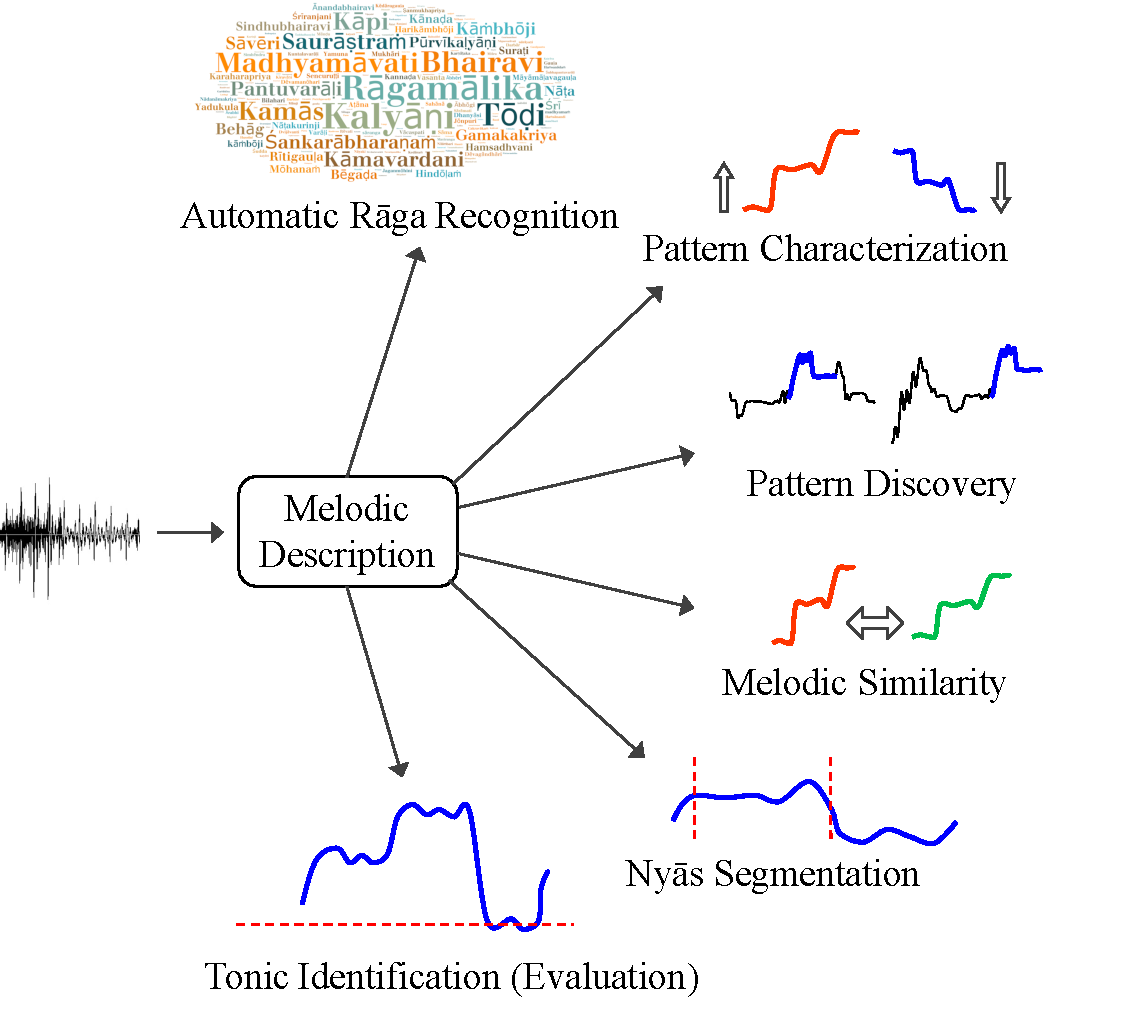
\includegraphics[width=\figSizeSeventyFive]{ch01_introduction/figures/tasks.pdf}
	\end{center}
	\caption[Computational melodic analyses addressed in this thesis]{Computational tasks within melodic analysis of \gls{iam} that are addressed in this thesis.}
	\label{fig:tasks}
\end{figure}

Finally, we aim to investigate one of the most studied and relevant topics in computational analysis of \gls{iam}, automatic \gls{raga} recognition. Our goal is to devise an approach that can successfully utilize both the tonal and the temporal characteristics of melody to perform the task. 

Our work aligns with the philosophy of open-access and reproducible research. The data and the code pertaining to this thesis is made publicly available online (\appref{app:resources}). 

\section{Thesis Outline}
\label{sec:intro_thesis_outline}

There are eight chapters in this thesis, wherein the primary contributions are contained in Chapter 3 to 6. Each of these chapters contains an introduction, the main body and a summary of the key results and conclusions. A significant amount of the content in these chapters is derived from our publications~\cite{Gulati2014Tonic,gulati2014Landmark,gulati_SITIS_2014,gulati_ICASSP2015,gulati_ISMIR_2015,gulati_communities_2016,gulatiphrase_2016,gulati_tdms_2016}. Most of the work in these papers is done in collaboration with other researchers and musicians, which is duly indicated wherever required. 

In \chapref{chap:background}, we provide an overview of the music and scientific background, with emphasis on the existing literature relevant to the work presented in this thesis. We start with a brief introduction to \gls{iam} and its music concepts pertaining to melody (\secref{sec:music_background}). We present our review of current computational approaches for tonic identification, \gls{raga} recognition and melodic pattern processing in the context of \gls{iam} (\secref{sec:background_relevant_work_iam}). We critically analyze and compare these approaches in terms of algorithmic design and evaluation methodology, in which we highlight their shortcomings and identify potential avenues of scientific contributions. In addition, we also present a brief review of the existing literature on tonality modeling and pattern processing in \gls{mir}, covering topics such as structural segmentation, motivic analysis and \gls{qbh} (\secref{sec:background_relevant_work_other_music}).

In \chapref{chap:corpus_music_corpora_and_datasets}, we describe the \gls{iam} corpora and different test datasets that are curated as a part of our work within the CompMusic project. We enumerate the set of design criterion followed to compile the music corpora and present a short evaluation of the goodness of the corpora with respect to these criterion (\secref{sec:corpus_criterion_for_corpora}). Subsequently, a detailed description of a number of test datasets used for evaluations in this thesis is provided (\secref{sec:corpus_test_datasets}). 

%The structure of the remaining part of the thesis is closely linked with the different computational tasks addressed in our work, which are summarized in~\figref{fig:tasks}. 

In \chapref{chap:data_preprocessing}, we describe the processes followed to extract relevant melody descriptors and melody representations that are used by the methods described in the subsequent chapters. We start with a comparative evaluation of different tonic identification approaches to select the best approach to work with in this thesis (\secref{sec:data_preprocessing_tonic_identification}). Subsequently, we describe the procedures followed for extracting and post-processing predominant pitch from audio recordings (\secref{sec:data_preprocessing_melody_processing}). Taking this low-level melody representation and the tonal context provided by the tonic we begin to perform higher level melodic analyses. We present an approach to segment melodies based on the concept of \gls{nyas} \glspl{svara}, which serve as landmarks that demarcate melodic patterns in Hindustani music (\secref{sec:pre_processing_nyas_segmentation}). We then describe the processing steps applied to segment solo percussion sections, \glspl{tani}, in performances of Carnatic music (\secref{sec:pre_processing_tani_segmentation}). Such sections need to be discarded in the pre-processing stage of all our melodic analysis approaches. 

In \chapref{chap:melodic_pattern_processing}, we present our main contributions and describe approaches for different computational tasks within melodic pattern processing. There are three related tasks addressed in this chapter, melodic similarity computation, pattern discovery and pattern characterization. We first investigate different choices of melody representation, distance measure and normalization strategy for computing melodic similarity in the context of \gls{raga} motifs in \gls{iam} (\secref{sec:patterns_evaluation_of_similarity_measures}). It includes an exhaustive evaluation of different procedures and their parameter settings commonly used for this task. We subsequently describe ways to improve melodic similarity by exploiting peculiar characteristics of melodies in \gls{iam} (\secref{sec:patterns_improving_melodic_similarity}). Having learned the optimal set of procedures and system parameters in a supervised setup, we then utilize this knowledge for discovering melodic patterns using an unsupervised methodology (\secref{sec:patterns_melodic_pattern_discovery}). Finally, we describe our approach to characterize the discovered melodic patterns in order to identify \gls{raga} motifs (\secref{sec:patterns_characterization_of_melodic_patterns}). 

In \chapref{chap:raga_recognition}, we present the other significant part of our scientific contributions in the thesis. This chapter addresses one of the most studied topics in computational analyses of \gls{iam}, automatic \gls{raga} recognition, for which we propose two novel approaches. Our first approach utilizes the discovered melodic patterns and employs vector space modeling techniques to perform this task (\secref{sec:pattern_based_raga_recognition}). Our second approach uses a novel melodic representation, the \gls{tdms}, which encodes both the tonal and the temporal aspects of melodies that are relevant to characterize \glspl{raga} (\secref{sec:tdms_raga_recognition}). We evaluate these methods and compare their performance with the state of the art methods using the largest datasets ever used for this task, wherein they outperform state of the art by large margins. Results prove the feasibility and effectiveness of using melodic patterns and \gls{tdms} representations of melody for \gls{raga} recognition on sizable datasets.

In \chapref{chap:applicatoins}, we present demos and a few concrete examples of applications that utilize the outcomes of our research work presented in this thesis. In particular, we introduce Dunya, a system that consolidates and provides access to the data, tools and technology developed in the CompMusic project (\secref{sec:applications_dunya}). In order to demonstrate the outcome of our melodic pattern discovery and \gls{raga} recognition approaches more directly, we present web-based demos (\secref{sec:demos}). To emphasize the utility of our work in a commercial context, we present two mobile applications: \gls{saraga}, which provides an enhanced music listening experience, and \gls{riyaz}, which facilitates self-paced learning of both Hindustani and Carnatic music (\secref{sec:mobile_apps_camut}). 

Finally, in \chapref{chap:summary_future_work} we present an overall summary of the thesis, list our main contributions, and discuss possible future perspectives for melodic description in \gls{iam}. 

This thesis also contains four appendix sections. In \appref{app:mypapers}, we list the relevant publications by the author. In \appref{app:resources}, we provide links to the relevant resources pertaining to our work such as music corpora, datasets, code, and other relevant tools. All the additional figures and tables that help in a better interpretation of our evaluation results are contained in~\appref{app:additional_material}. \appref{app:glossary} presents the glossary of the abbreviations and other terms used in this thesis. 



%\cleartorecto%!TEX root = ../thesis_a4.tex

\chapter{Background}
\label{chap:background}

\section{Introduction}

In this chapter we provide the relevant music and scientific background for the work presented in this dissertation. We start with a brief discussion on the terminology used in this thesis (\secref{sec:background_terminology}). Subsequently, we provide an overview of the selected music concepts relevant to better understand our work (\secref{sec:music_background}). We then present a review of the literature related with the topics addressed in this thesis. We first present relevant work done in computational analysis of \gls{iam} (SEction XX), which includes approaches for tonic identification, automatic \gls{raga} recognition and melodic pattern processing. Then, we present work done for other music traditions within \gls{mir} on topics covering melodic pattern processing and key recognition (\secref{sec:background_relevant_work_other_music}). Finally, we provide an overview of the select scientific concepts in information retrieval, time-series analysis, complex networks and statistics (\secref{sec:background_scientific_background}). We conclude this chapter by providing a summary of the literature review, wherein we highlight the shortcomings of the existing approaches, and identify some possible venues for scientific contribution (\secref{sec:background_summary}). 

\section{Terminology}
\label{sec:background_terminology}

In this section we provide working definition of the selected terms we have used throughout the thesis. Since the thesis focuses on the melodic description of \gls{iam}, it is important to clearly understand the meaning of melody in the context of this thesis. Our aim here is not to formally define melody in an universal sense, which as we see from the literature has been a challenge in itself, with almost every definition falling short of considering some aspect or the other XXXX. It would not be an overstatement to say that there is no agreed definition of melody that suits every context. For a review of interesting definitions of melody we refer to XXXX. Before we present the definition of melody that we consider in this work, it is important to understand the performance or concert setup in \gls{iam}. Since this music tradition is performance-based, even the studio recordings follow the same setup. Performances in \gls{iam} have a clearly defined concept of a lead artist, who plays the central role (also literally positioned in the center of the stage) and all other instruments are considered the accompaniments. In this context, mergin relevant parts of the definitions given by~\cite{paiva2006melody,kim2000analysis,levitin2002memory} covers to a large extent the scope of melody in \gls{iam}. Their definitions in the respective order are: \textquote{``\textit{the dominant individual pitched line in a musical ensemble}''} and \textquote{``\textit{an auditory object that emerges from a series of transformations along the six dimensions: pitch, tempo, timbre, loudness, spatial location, and reverberant environment}''}.  The first definition falls short of considering several other dimensions of sound such as timbre and loudness that are important in perception and production of melody, which are taken into account in the second definition. The concept of audio as a mixture of sounds from multiple instruments (`\textit{ensemble}') is missing in the second definition, which the first definition takes into account. The idea of continuity and smoothness of melody is expressed by `\textit{line}' in the former and by `\textit{series of transformations}' in the latter. If we combine these two definitions we can rewrite our working definition as \textquote{``\textit{an auditory object that emerges from a continuous series of transformations along the six dimensions: pitch, tempo, timbre, loudness, spatial location, and reverberant environment, by the dominant individual sound source in a music ensemble}''}. Although, we only consider the pitch dimension of melody in this thesis. Thus, loosely speaking, for all practical purposes within the scope of this thesis, we represent melody by a continuous pitch time-series corresponding to the lead artist in an audio recording, also referred to as predominant pitch in the subsequent chapters. This definition does not explicitly take into account the rare case of two lead artists. Since in a majority of such cases the two lead sound sources are active sequentially in time, our definition encompasses this scenario by considering the active sound source as dominant. \TODO{please make this shit better, these thigns are so confusing and broad}

Now that we have a working definition of melody, we proceed to define the scope of the terms such as melodic patterns, phrases and motifs in this thesis, and disambiguate them with other seemingly synonymous terms such as melodic fragment and segment. Melodic fragment or melodic segment in this thesis refers to a continuous subsequence of the pitch sequence. It does not entail any musical relevance in terms of the boundaries or the length of the subsequence. By a melodic pattern we refer to a repeating melodic fragment, where the scope and the meaning of repetition is based on the perceived melodic similarity. Across repetitions, a melodic fragment can undergo a series of time and pitch transformations allowed within the periphery of melodic framework (\gls{raga} in our case) without altering the identity of the melodic unit. Also, the melodic similarity here refers to the perceived similarity between melodic fragments when heard in isolation, as the local melodic context can influence the perception of similarity. Melodic patterns in this thesis do not entail any particular musical significance in terms them being characteristic of a melodic concept in \gls{iam}. The terms melodic pattens, fragments and segments are more from the perspective of signal or the time-series. Melodic phrases on the other hand are used in the context of music, as being a unit of melody which encapsulate an idea or a musical thought by an artist. Melodic motif is further high-level concept and we use it to refer to a particular type of characteristic patterns, in out thesis of \glspl{raga}, \gls{raga} motifs. 


The word polyphonic in the context of audio recordings signifies that the recordings consists of a mixtue of multiple instruments playing simultaneously.


\section{Music Background}
\label{sec:music_background}

\subsection{Indian Art Music}

\subsection{Melodies in Indian Art Music}

\subsubsection{Tonic in Indian art music}
\label{sec:background_tonic_in_iam}

\subsubsection{Svaras}

\subsubsection{Aroh-Avroh}

\subsubsection{Gamakas and Ornaments}

\subsubsection{Raga in Indian Art Music}

\paragraph{Phase-based and Scale-based ragas}
\paragraph{Allied ragas}

\subsubsection{Characteristic Melodic Phrases}

\subsubsection{Chalan}

\subsubsection{Nyas}
\label{sec:backgroung_nyas_description}

Dey presents various interpretations and perspectives on the concept of ny\={a}s in Hindustani music according to ancient, medieval and modern authors~\cite{Dey2008}. In the context of its current form, the author describes ny\={a}s as that process in a performance of a r\={a}g where an artist pauses on a particular \gls{svara}\footnote{The seven solf\`{e}ge symbols used in Indian art music are termed as \glspl{svara}. It is analogous to note in western music but conceptually different.}, in order to build and subsequently sustain the format of a r\={a}g, the melodic framework in Indian art music~\cite[p. 70]{Dey2008}\cite{KKG_SS13}. Dey elaborates the concept of ny\={a}s in terms of action, subject, medium, purpose and effect associated with it. Typically, occurrence of a ny\={a}s delimits melodic phrases (motifs), which constitute one of the most important characteristic of a r\={a}g. Analysis of ny\={a}s is thus a crucial step towards melodic analysis of Hindustani music. In particular, automatically detecting occurrences of ny\={a}s (from now on referred as ny\={a}s segments) will aid in computational analyses such as melody segmentation, motif discovery, r\={a}g recognition and music transcription~\cite{GopalJNMR2012, Rao2014}. However, detection of ny\={a}s segments is a challenging computational task, as the prescriptive definition of ny\={a}s is very broad, and there are no fixed set of explicit rules to quantify this concept~\cite[p. 73]{Dey2008}. It is through rigorous practice that a seasoned artist acquires perfection in the usage of ny\={a}s, complying to the r\={a}g grammar and exploring creativity through improvisation at the same time. 

\subsubsection{Recurring Melodic Patterns in IAM}


\section{Relevant Work in Indian Art Music}
\label{sec:background_relevant_work_iam}


\subsection{Tonic Identification}
\label{sec:background_relevant_work_tonic_identification}

In this section we provide a detailed review of the existing methods for tonic identification in audio recordings of \gls{iam}. The main objective of this review is to break down the methodology used across methods into a common set of processing blocks, and subsequently analyze different methods in terms of these blocks. Since in this thesis we also perform an extensive comparative evaluation of a number of these methods (\secref{sec:data_preprocessing_tonic_identification}), we review the methods in detail. In order to better interpret the output of these methods and to relate them with the processing steps and parameter choices, we provide the necessary implementation details, wherever required.


Identification of tonic pitch of the lead artist in an audio recording is a crucial first step in tonal analysis of \gls{iam} (\secref{sec:background_tonic_in_iam}). Knowing the tonic pitch used in an audio recording enables a meaningful comparison of melodies across different artists and their recordings. In this section we review existing approaches for automatic tonic identification in audio collections of \gls{iam}. 

As mentioned, there have been various efforts to automatically identify the tonic pitch of the lead artist in a performance of Indian art music~\citep{salamon2012multipitch,gulati2012two,bellur2012knowledge,ranjani2011carnatic,Sengupta2005b}. These approaches mainly differ in terms of the musical cues that they utilize to identify the tonic, the amount of input audio data used to perform this task and the type of music material they are devised for (Hindustani or Carnatic, vocal or
instrumental, etc.). Despite the differences, all these approaches can be divided into three main processing blocks, as shown in~\figref{fig:tonic_identification_general_block_diagram}. The only exception to this schema is the approach proposed by~\cite{Sengupta2005b}.

\begin{figure}
	\begin{center}
		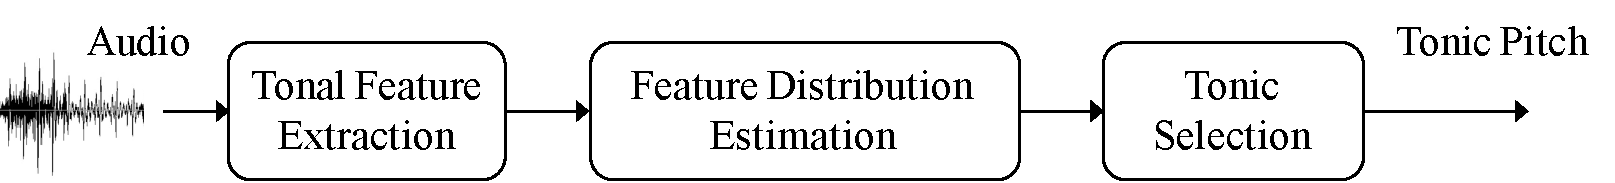
\includegraphics[width=\figSizeNinety]{ch02_background/figures/tonic_identification_block_diagram.pdf}
	\end{center}
	\caption[General block diagram of the processing steps used by tonic identification
	approaches.]{General block diagram of the processing steps used by tonic identification
		approaches.}
	\label{fig:tonic_identification_general_block_diagram}
\end{figure}


In all the aforementioned approaches, the three main processing blocks are the following: feature extraction, feature distribution estimation and tonic selection. Since the task of tonic identification involves an analysis of the tonal content of the audio signal, the features extracted in the first block are always pitch related. In the second block, an estimate of the distribution of these features is obtained using either Parzen window based density estimation or by constructing a histogram. The feature distribution is then used in the third block to identify the tonic. The peaks of the distribution correspond to the most salient pitch values used in the performance (usually the \glspl{svara} of the \gls{raga}), one of which corresponds to the tonic pitch. As the most salient peak in the distribution is not guaranteed to be the tonic, various techniques are applied to select the peak that corresponds to the tonic.

{\renewcommand{\arraystretch}{1.5}
	\begin{sidewaystable} 
		\begin{centering}
			\begin{tabular}{ c c c c }
				\tabletop			
				Method 	&	Features	&	Feature Distribution	&	Tonic Selection \\
				\tablemid			
				\acrshort{tonicid_sengupta} \citep{Sengupta2005b}	&	Pitch \citep{AKDatta_1996} & N/A & Error minimization\\
				
				\acrshort{tonicid_ranjani_1}/\acrshort{tonicid_ranjani_2} \citep{ranjani2011carnatic}	&	Pitch \citep{BoersmaPaul2001} & Parzen-window-based \acrshort{pde}  & GMM fitting\\
				
				\acrshort{tonicid_justin} \citep{salamon2012multipitch} & Multi-pitch salience \citep{Salamon2011} & Multi-pitch histogram & Decision tree\\
				
				\acrshort{tonicid_sankalp} \citep{gulati2012two}	& Multi-pitch salience  \citep{Salamon2011} & Multi-pitch histogram & Decision tree\\
				
				&	Predominant melody \citep{Salamon2012} & Pitch histogram & Decision tree\\
				
				\acrshort{tonicid_ashwin_1} \citep{bellur2012knowledge}	&	Pitch \citep{DeCheveigne2002}	&  \acrshort{gd} histogram & Highest peak\\
				
				\acrshort{tonicid_ashwin_2} \citep{bellur2012knowledge}	&	Pitch \citep{DeCheveigne2002}	& 	GD histogram	&
				Template matching\\
				
				\acrshort{tonicid_ashwin_2} \citep{bellur2012knowledge}	&	Pitch \citep{DeCheveigne2002}	& 	GD histogram
				& Highest peak\\
				
				\acrshort{tonicid_chordia}	& 	& 	& \\			
				
				\tablebot			
			\end{tabular}
			
			\caption[Summary of existing tonic identification approaches.]{Summary of existing tonic identification approaches.}
			\label{tab:pre_processing_tonic_identification_summary_methods}
			\par \end{centering}	
	\end{sidewaystable}
	
	
In \tabref{tab:pre_processing_tonic_identification_summary_methods} we provide a summary of the existing methods for tonic identification. The common processing blocks and the main differences between them become evident from this table. A detailed review of these methods in terms of the three processing stages as shown in \figref{fig:tonic_identification_general_block_diagram} is done in~\cite{Gulati2014Tonic}. For a more detailed description of these methods we refer to their respective publications listed in Table \tabref{tab:pre_processing_tonic_identification_summary_methods}. 


\subsubsection{Tonal Feature Extraction}
\label{Feature Extraction}

In the tonal feature extraction block (\figref{fig:tonic_identification_general_block_diagram}), the algorithms extract pitch-related
features from the audio signal for further processing. With the exception of \cite{SalamonSankalp2012,SGulatiIstanbul2012}, all approaches use a single feature, the predominant pitch in the audio. Note that whilst pitch and fundamental frequency ($f_0$) are not the same (the former being a perceptual phenomenon and the latter a physical quantity), for the purpose of tonic identification the $f_0$ is considered a reliable representation of pitch. Unlike these approaches, Salamon \cite{SalamonSankalp2012} uses a multi-pitch salience feature in order to exploit the tonal information provided by the drone instrument. Finally, Gulati \cite{SGulatiIstanbul2012} uses both the multi-pitch salience feature and the predominant melody. 

We now provide an overview of the algorithms used by the different approaches mentioned above for extracting $f_0$ and multi-pitch salience from audio recordings. \cite{ranjani2011carnatic} use the Praat software\footnote{Version 5.3.} \cite{BoersmaPaul2001} to obtain the pitch contours. The software implements the algorithm by~\cite{boersma1993accurate}, which is primarily proposed for speech signals and has also been used for monophonic music recordings in the past. \cite{Ashwin_Istanbul2012} uses an \gls{amdf} based pitch estimation algorithm, YIN, proposed by~\cite{DeCheveigne2002}. YIN is mainly developed for speech signals. As~\cite{DeCheveigne2002} make a remark,  the algorithm is informally tested on music and yet to be evaluated on polyphonic music. However, YIN has been used in a number of studies in \gls{mir} for pitch estimation from polyphonic music signals REF. \cite{Sengupta2005b} use a method based on \gls{psa} proposed by~\cite{AKDatta_1996} for extracting the $f_0$. Subsequently, a steady state detection is applied to the pitch contours in order to consider only the steady note regions for the analysis. Only segments of the pitch contour with a steady-state duration of at least 60 ms are used. It should be noted that this study was carried out using solo vocal performances (monophonic audio), which were carefully recorded in a studio without any kind of accompaniment present in the audio.

One of the possible caveats of the aforementioned pitch (strictly speaking, $f_0$) estimation methods is that they are all designed for monophonic signals containing a single sound source. This means that the number of estimation errors could increase as we add more instruments into the mixture. While due to the heterophonic nature of \gls{iam} and the prominent lead voice monophonic pitch trackers often manage to detect the $f_0$ of the lead artist even in the presence of accompaniment instruments. One way of overcoming this problem is by using a predominant pitch estimation algorithm. \cite{gulati2012two} use the method proposed by~\cite{Salamon2012} for estimating the pitch sequence of the predominant melody from the audio signal. \cite{gulati2012two} exploit the pitch information of the melody in the second stage of their approach to identify the specific octave of the tonic pitch (the tonic pitch-class is identified during the first stage of the algorithm).

As noted earlier, some recently proposed methods for tonic identification~\citep{salamon2012multipitch,gulati2012two} use a multi-pitch approach. Instead of extracting the predominant melodic component from the audio signal, the methods compute a multi-pitch time-frequency representation of pitch salience over time~\citep{Salamon2011}. The motivation for using multi-pitch analysis is twofold: first, as noted earlier, the music material under investigation is non-monophonic (includes many instruments playing simultaneously). Second, the tonic is continuously reinforced by the drone instrument, and this important cue can not be exploited by only extracting a single pitch value for each frame of the audio recording. To illustrate this point, in~\figref{fig:2HarmonicSeries} we display the spectrogram of a short audio excerpt of Hindustani music. Two types of harmonic series are clearly visible in the plot: the first consists of nearly straight lines and corresponds to the drone instrument (playing Sa and Pa). The second harmonic series (which start approximately at time 1 s) corresponds to the voice of the lead performer. Since the drone instrument is constantly present in the signal, a histogram of the peaks of the salience function will have prominent peaks at the pitches of the drone instrument, and this is exploited by \cite{SalamonSankalp2012,SGulatiIstanbul2012} for identifying the tonic. The main difference between the two approaches is that whilst~\citep{salamon2012multipitch} directly identifies the tonic pitch from the histogram, \cite{gulati2012two} divides the task into two stages: first the tonic pitch-class is identified using an extension of \cite{salamon2012multipitch}, and then the correct tonic octave is identified using the predominant melody information (see~\cite{Gulati2014Tonic} for further details).

\begin{figure}
	\begin{center}
		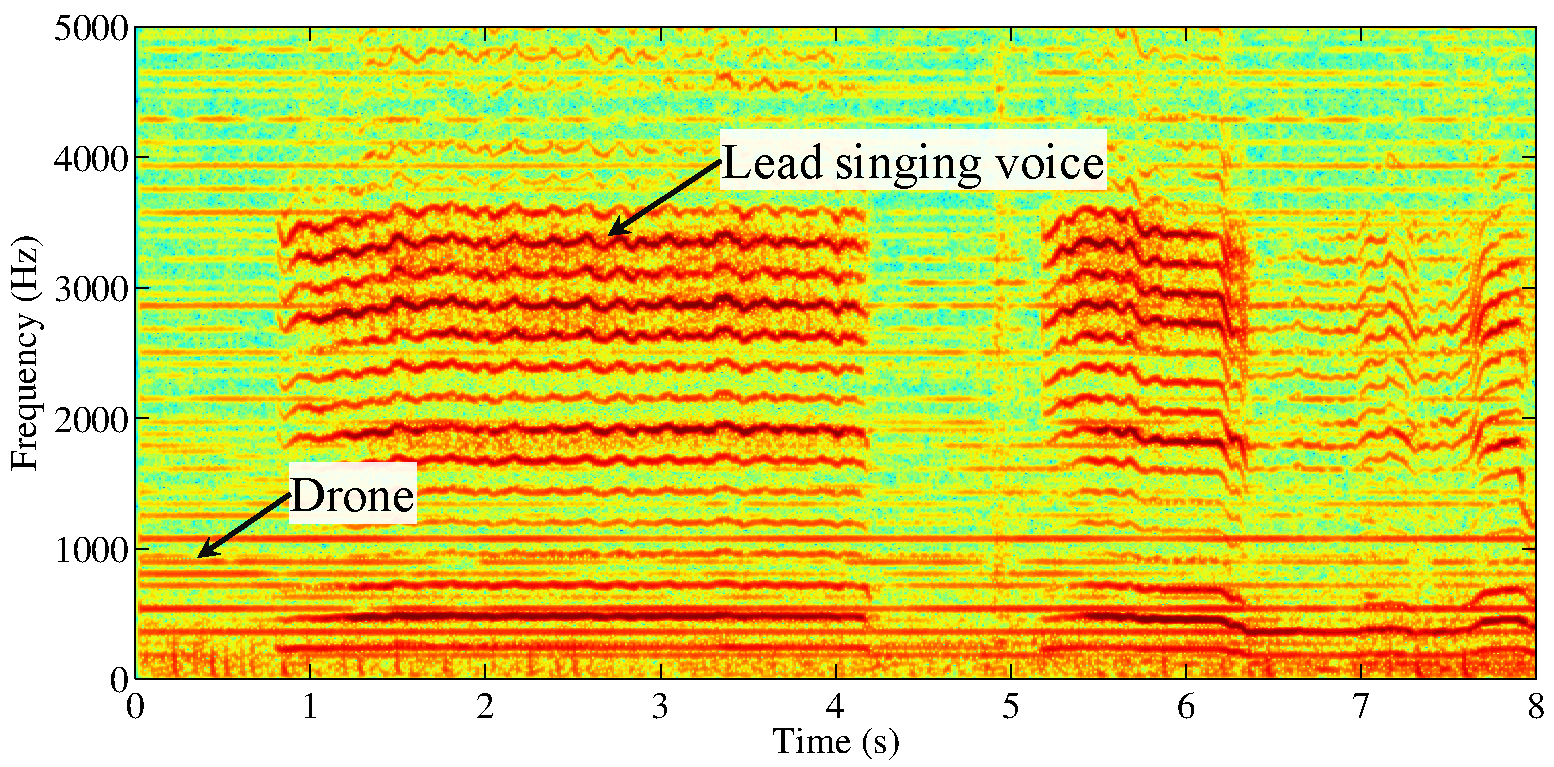
\includegraphics[width=\figSizeNinety]{ch02_background/figures/2HarmonicSeries.pdf}
	\end{center}
	\caption{Spectrogram of an excerpt of Hindustani music with two clearly visible types of harmonic series, one belonging to the drone and the other to the lead voice.}
	\label{fig:2HarmonicSeries}
\end{figure}


\subsubsection{Feature Distribution Estimation}
\label{sec:background_tonic_feature_distribution_estimation}

The tonal features extracted by the different tonic identification approaches are subsequently analyzed in a cumulative manner (cf.~block two in Figure \ref{fig:tonic_identification_general_block_diagram}). The pitch values from all analysis frames (whether a single value is computed per frame or multiple values) are aggregated into a pitch distribution function, which reflects the (possibly weighted) rate of occurrence of different pitch values in the entire audio excerpt. The peaks of the pitch distribution function represent the most frequent (or salient if weighting is used) pitches in the recording, one of which will be the tonic. The only exception is the approach proposed by~\cite{Sengupta2005b}, which instead of analyzing the distribution of the features, computes an aggregate error function in order to select the tonic. The methods used by the different tonic identification approaches for estimating the pitch distribution function are described below.

In~\cite{salamon2012multipitch,gulati2012two}, the pitch values of the peaks of the salience function in every frame are aggregated into a histogram. The top 10 peaks in every frame are used, in this way ensuring that in addition to the lead instrument/voice, the pitch content of other accompanying instruments is also captured, most importantly the notes played by the drone instrument. The frequency range considered for selecting the peaks of the salience function for constructing the histogram is restricted to 100-370 Hz (note that the typical frequency range for the tonic 100-260 Hz). The reason for computing the histogram beyond 260 Hz even though the tonic rarely goes above this frequency is that in some cases the aforementioned methods can exploit the presence of a peak corresponding to the fifth/fourth (Pa/Ma) above the tonic in order identify the tonic pitch. Since in many cases the lead voice/instrument is considerably louder than the drone sound, the weights of the salience peaks are ignored when computing the histogram, meaning only the rate of occurrence is taken into account. As noted earlier, the result is that the pitches produced by the drone instrument (the tonic and Pa, Ma or \gls{ni}) manifest in the form of high peaks in the histogram, since the drone sounds continually in the recording. The resulting pitch distribution thus depends heavily on the notes of the drone instrument. This would not be the case if we only considered the predominant melody for computing the histogram, in which case the pitch distribution would depend on the chosen \gls{raga}, thus increasing the complexity of identifying the tonic.

\begin{figure}
	\begin{center}
		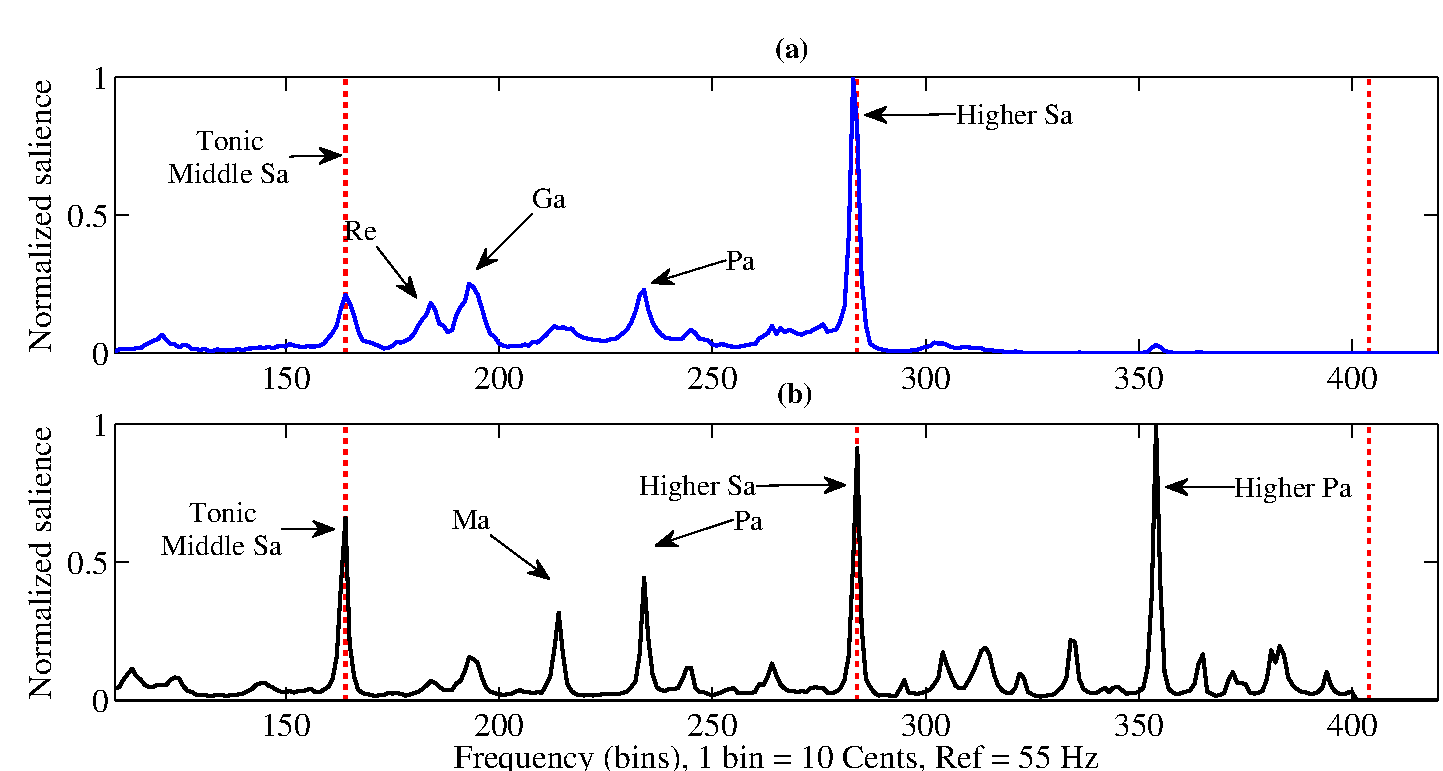
\includegraphics[width=\figSizeNinety]{ch02_background/figures/Histogram_Melody_Multipitch.pdf}
	\end{center}
	\caption[Comparison of the histograms constructed using different methods]{Pitch histograms for the same excerpt constructed using (a) predominant melody (in blue) and (b) peaks of a multi-pitch salience function (in black). The tonic pitch-class locations are indicated with red dotted lines.}
	\label{fig:background_pitch_histograms_multipitch}
\end{figure}

In Figure \ref{fig:background_pitch_histograms_multipitch} we display two pitch histograms, computed using (a) the pitch of the predominant melody and (b) the peaks of a multi-pitch salience function. Both histograms are computed from the same three-minute audio excerpt. We see that in the histogram computed using the predominant melody (a), the prominent peaks correspond to \glspl{svara} Sa, Ga and Re (the prominent \glspl{svara} of \gls{raga} \textit{Sindh Bhairav\={i}} ), whereas in the multi-pitch histogram (b), the top three peaks correspond to Sa (in two octaves) and Pa, which are the prominent \glspl{svara} produced by the drone instrument. 

In~\cite{Ashwin_Istanbul2012}, a histogram is constructed using a frequency range of 40-800 Hz with a 1 Hz resolution and later post processed using a group delay function. The authors show that by assuming that the constructed pitch histogram is the squared magnitude of resonators in parallel, group delay functions can be applied to obtain a better resolution for the peaks in the resulting histogram. It is also shown that a group delay function accentuates peaks with lesser bandwidths. Given that the \gls{shadja} (tonic pitch-class) and panchama (3/2 of the tonic pitch-class) in all octaves are relatively less inflected, this characteristic of the group delay function is shown to be beneficial for improving the accuracy of tonic identification. The processed histograms are referred to as \gls{gd} histograms.

\cite{Ashwin_Istanbul2012} also propose the concept of segmented histograms. In order to exploit the omnipresence of the \gls{shadja},  it is proposed that, given the pitch contour for an item of music, the contour is segmented into smaller units and a \gls{gd} histogram is constructed for each of these smaller units. Given that \gls{shadja} will be present in all the units, the peak corresponding to the \gls{shadja} will be enhanced in the corresponding \gls{gd} histograms. The individual histograms are then multiplied bin-wise. This also helps in reducing the height of the non \gls{shadja} peaks which might not be present in all the segments. Tonic selection is then performed on the resulting histogram, referred to as the segmented \gls{gd} histogram.

Instead of using a histogram, \cite{ranjani2011carnatic} use a Parzen window estimator to compute a pitch density function~\citep{Bishop,DudaHart2000}. Parzen window estimators (or kernel density estimators) are non-parametric density estimators. The choice of kernel function can control the smoothness of the estimated density. They are widely used as an alternative to histograms to alleviate the artificial discontinuities at the boundaries of the bins of the histogram, and aid in a smoother peak picking process. In addition, they do not require partitioning of data into distinct bins. \cite{ranjani2011carnatic} use parzen window estimators with Gaussian kernels for estimating the density of the extracted pitch frequencies.


\subsubsection{Tonic selection}
\label{Tonic Selection}

In the previous section we discussed different ways to compute the pitch distribution function. This section presents the last processing block shown in~\figref{fig:tonic_identification_general_block_diagram}, where the pitch distribution function is used to identify the tonic pitch. The peaks of the pitch distribution function correspond to the most frequent (or salient) pitches present in the audio signal. Depending on how the pitch distribution is computed the peaks will coincide with the \glspl{svara} of the \gls{raga} used in the rendition or with the \glspl{svara} produced by the drone instrument. The problem of tonic identification is thus reduced to selecting the peak of the distribution that corresponds to the tonic of the lead artist. As noted earlier, the peak corresponding to the tonic pitch is not always the highest peak in the distribution. For this reason, various strategies are have been proposed for analyzing the pitch distribution and selecting the peak that corresponds to the tonic. The complexity of the approaches varies from simply selecting the highest peak of the histogram to the application of machine learning algorithms in order to automatically learn the best set of rules for selecting the tonic peak. The different tonic selection strategies used in the literature are presented below.

\cite{Ranjani2011} model the pitch distribution using semi-continuous Gaussian mixtures~\cite{Huang2001}, motivated by the following two musical cues in Indian art music: first, the relative positions of the \glspl{svara} with respect to the tonic hover around a mean ratio \cite{Krishnaswamy2003} and second, the \gls{shadja} (tonic pitch-class) and panchama (fifth of the tonic pitch-class) are the prakrthi \glspl{svara} which means they are sung/played without any inflections \cite{Manikandan2004,Krishnaswamyicassp2003}. Peaks of the pitch density function within a suitable pitch range are selected as possible tonic candidates. The variance of the pitch distribution around the peaks is estimated by modeling each tonic candidate (i.e.~peak) with a Gaussian distribution. As noted above, one of the key characteristics of \gls{shadja} and panchama is that they do not vary (in pitch) throughout the performance. Thus, the parameters of the Gaussian model are used to infer the correct tonic candidate. The pitch range used for selecting tonic candidates is 100\,-\,250\,Hz. When the editorial metadata of the audio recording is known, the pitch range is further constrained depending on the gender of the lead artist. The range for male singers is set to 100\,-\,195 Hz and for female singers is set to 135\,-\,250 Hz.

\cite{salamon2012multipitch,gulati2012two} use a classification based approach to identify the peak of the multi-pitch histogram that corresponds to the tonic pitch \cite{salamon2012multipitch} or tonic pitch-class \cite{gulati2012two}. Since all the pitches in a performance are in relation to the tonic, the relationships between the peaks of the histogram (height and distance) are used to compute a set of features, which are then used to train a classifier for identifying which peak corresponds to the tonic. In this way, rather than having to manually define a template for selecting the tonic, an optimal set of rules are learned automatically using machine learning. The authors extract height and distance related features for the top 10 peaks in the multi-pitch histogram. The authors show that for the tonic identification task the C4.5 decision tree classifier~\cite{Quinlan:1993:CPM:152181} yields the highest classification accuracy. 

\cite{SGulatiIstanbul2012} uses a similar classification-based approach to first identify the peak of the histogram that corresponds to the tonic pitch-class. The correct tonic octave is then determined in the second stage of processing, which is also classification-based. For every candidate tonic pitch (candidates have the same pitch class but are in
different octaves) a set of 25 features is computed. The features are the values of the melody histogram at 25 equally spaced locations spanning two octaves centered around the tonic pitch candidate. The classification is a two-class problem: either the pitch candidate is in the correct octave, or it is not. As done in~\cite{salamon2012multipitch}, a C4.5 decision tree is trained using the Weka data-mining software for the classification. For a detailed description of the method we refer to~\cite{SGulati_MThesis2012}.

\cite{Sengupta2005b} use an error minimization technique to identify the tonic. This is a brute force approach: a large number of pitch values within a pre-defined frequency range are considered as candidates for the tonic pitch. A cumulative deviation is computed between the steady state regions of the pitch contour (described in~\secref{sec:background_tonic_feature_distribution_estimation}) and the pitch values of the closest notes to these regions, which are obtained using three different tuning schemas given a tonic candidate. The tonic candidate which results in the minimum deviation is selected as the tonic of the musical excerpt.

\cite{Ashwin_Istanbul2012} propose a simple approach, picking the highest peak of the pitch distribution as the tonic. In two out of the three proposed variants of their method, the bin value of the highest peak of the segmented \gls{gd} pitch histogram is selected as the tonic pitch. The frequency range of the histogram is restricted to 100-250\,Hz. When the gender information of the lead artist for an audio recording is available, this range is further restricted. In addition to the simple highest peak approach, \cite{Ashwin_Istanbul2012} also propose a template matching process to identify tonic. This procedure is comparable to the Semi-continuous GMM fitting proposed by \cite{Ranjani2011}, which exploits the smaller degree of pitch variation around \gls{shadja} and panchama. The template that authors use to identify the tonic candidate uses three octaves and consider the pitch distribution values at tonic and its fifth (Pa) in different octaves. For more information we refer to~\cite{Gulati2014Tonic}.


\TODO{A concluding paragraph of this section, motivating the need for a thorough evaluation.}


\subsection{\Glsentrytext{raga} Recognition}
\label{sec:sota_raga_recognition}


\begin{sidewaystable}
	\begin{threeparttable} 
		\ra{1.1}
		\setlength{\tabcolsep}{2pt}
		\small
		\begin{centering}
			\begin{tabular}{l L{2.5cm} L{2cm} L{2.5cm} L{2.5cm} L{2.5cm} L{2.5cm} L{2.5cm}}
				\tabletop
				& Svara set & Svara salience & Svara intonation & \Gls{arohana}-\gls{avrohana} & Melodic phrases & Svara discretization & Temporal aspects\tabularnewline
				\tablemid
				\cite{pandey2003tansen} &  &  &  & $\bullet$ & $\bullet$ & Yes & $\bullet$\tabularnewline
				\cite{chordia2007raag} & $\bullet$ & $\bullet$ &  & $\bullet$ &  & Yes & $\bullet$\tabularnewline
				\cite{belle2009raga} & $\bullet$ & $\bullet$ & $\bullet$ &  &  & No & \tabularnewline
				\cite{Shetty2009} & $\bullet$ &  &  & $\bullet$ &  & Yes & $\bullet$\tabularnewline
				\cite{sridhar2009raga} & $\bullet$ &  &  & $\bullet$ &  & Yes & $\bullet$\tabularnewline
				\cite{koduri2011survey} & $\bullet$ & $\bullet$ &  &  &  & Yes & \tabularnewline
				\cite{ranjani2011carnatic} & $\bullet$ &  &  &  &  & No & \tabularnewline
				\cite{chakraborty2012object} & $\bullet$ &  &  &  &  & Yes & \tabularnewline
				\cite{koduri2012raga} & $\bullet$ & $\bullet$ & $\bullet$ &  &  & Both & \tabularnewline
				\cite{chordia2013joint} & $\bullet$ & $\bullet$ & $\bullet$ &  &  & No & \tabularnewline
				\cite{dighe2013scale} & $\bullet$ & $\bullet$ &  & $\bullet$ &  & Yes & $\bullet$\tabularnewline
				\cite{dighe2013swara} & $\bullet$ & $\bullet$ &  &  &  & Yes & \tabularnewline
				\cite{koduri2014intonation} & $\bullet$ & $\bullet$ & $\bullet$ &  &  & No & \tabularnewline
				\cite{kumar2014identifying} & $\bullet$ & $\bullet$ & $\bullet$ & $\bullet$ &  & Yes & $\bullet$\tabularnewline
				\cite{shrey_ISMIR_2015}\tnote{a} &  &  &  &  & $\bullet$ & No & $\bullet$\tabularnewline	
				\tablebot
			\end{tabular}
			\par \end{centering}
		
		\begin{tablenotes}
			\item[a] This method performs \gls{raga} verification and not recognition
		\end{tablenotes}
		\caption{\Gls{raga} recognition methods proposed in the literature along with the melodic characteristics they utilize to perform the task. We also indicate if a method uses a discrete \gls{svara} representation of melody. The methods are arranged in the chronological order. \TODO{review the approaches and verify, add abbreviations}}
		\label{tab:raga_recognition_methods_melodic_characteristics}
	\end{threeparttable}
\end{sidewaystable}


\begin{sidewaystable}
	\begin{threeparttable} 
		\tiny
		\ra{1.1}
		\begin{centering}
			\begin{tabular}{l l P{2cm} P{3cm} P{2.5cm} L{1cm} P{1.5cm} P{2cm}}
				\hline 
				& \textbf{Tonal Feature} & \textbf{Tonic } & \textbf{Feature} & \textbf{Recognition Method} & \textbf{\#Ragas} & \textbf{Dataset Size (Dur./Num)}\tnote{i} & \textbf{Audio Type}\tabularnewline
				\hline 
				\cite{pandey2003tansen} & \cite{BoersmaPaul2001}\tnote{p} & Fixed frequency & Svara sequence & \acrshort{hmm} and \acrshort{ngram} & 2 & NA / 31 & Monophonic\tabularnewline
				\cite{chordia2007raag} & \cite{sun2000pitch}\tnote{p} & Manual & PCD, PCDD & \acrshort{svm} classifier & 31 & 20 / 127 & Monophonic\tabularnewline
				\cite{belle2009raga} & \cite{rao2009improving}\tnote{p} & Manual & PD (parameterized) & \acrshort{knn} classifier & 4 & 0.6 / 10 & Polyphonic\tabularnewline
				\cite{Shetty2009} & \cite{sridhar_2006_svara}\tnote{p} & Fixed frequency & \#Svaras, its combinations, Vakra svaras & Neural Network classifier & 20 & NA / 90 & Monophonic\tabularnewline
				\cite{sridhar2009raga} & \cite{lee2006automatic}\tnote{p} & Singer identification & Svara set, its sequence & String matching & 3 & NA / 30 & Polyphonic\tabularnewline
				\cite{koduri2011survey} & \cite{rao2010vocal}\tnote{p} & Brute force & PCD & \acrshort{knn} classifier & 10 & 2.82 / 170 & Polypohonic\tabularnewline
				\cite{ranjani2011carnatic} & \cite{BoersmaPaul2001}\tnote{p} & GMM fitting & PDE & SC-GMM and Set matching & 7 & NA / 48 & Polyphonic\tabularnewline
				\cite{chakraborty2012object} & \cite{sengupta1990study}\tnote{p} & Error minimization & Svara set & Set matching & NA & NA / NA & NA\tabularnewline
				\cite{koduri2012raga} & \cite{Salamon2012}\tnote{p} & Multipitch-based & PCD variants & \acrshort{knn} classifier & 43 & NA / 215 & Polyphonic\tabularnewline
				\cite{chordia2013joint} & \cite{camacho2007swipe}\tnote{p} & Brute force & PCD variants & \acrshort{knn} and statistical classifiers & 31 & 20 / 127 & Monophonic\tabularnewline
				\cite{dighe2013scale} & Chroma~\citep{lartillot2008matlab}\tnote{c} & Brute force (Vadi-based) & Chroma, Timbre features & \acrshort{hmm}  & 4 & 9.33 / 56 & Polyphonic\tabularnewline
				\cite{dighe2013swara} & \citep{lartillot2008matlab}\tnote{c} & Brute force (Vadi-based) & PCD variant & Random Forest & 8 & 16.8 / 117 & Polyphonic\tabularnewline
				\cite{koduri2014intonation} & \cite{Salamon2012}\tnote{p} & Multipitch-based & PCD (parameterized)  & Several classifiers & ?? & ?? & Polyphonic\tabularnewline
				\cite{kumar2014identifying} & \cite{Salamon2012}\tnote{p} & Brute force & PCD + \acrshort{ngram} distribution & \acrshort{svm} classifier  & 10 & 2.82 / 170 & Polyphonic\tabularnewline
				\cite{shrey_ISMIR_2015}{*} & \cite{Salamon2012}\tnote{p} & Cepstrum-based & Pitch contours & LCSS with \acrshort{knn} & 30 & 3 / 254 & Polyophonic\tabularnewline
				\hline 
			\end{tabular}
			\par \end{centering}
		\begin{tablenotes}
			\item[i] In the case of multiple datasets we list the larger one
			\item[p] Pitch extraction algorithm
			\item[c] Chroma extraction algorithm
			\item[*] This method performs \gls{raga} verification and not recognition
		\end{tablenotes}
		\caption{Summary of the \Gls{raga} recognition methods proposed in the literature. The methods are arranged in the chronological order. \TODO{review the approaches and verify. Put specific resolution of PCD and mark if they used KDE based PCD? also make it consistent the vocabulary. Clean it further and use more meaningful descriptor names. Both Dighe paper use chroma feature...chromagram types...not PCD variant. Verify all these details..add abbreviations}}
		\label{tab:raga_recognition_methods_details}
	\end{threeparttable}
\end{sidewaystable}

In this section we present a critical review of the existing computational approaches for \gls{raga} recognition in audio collections of \gls{iam}. Our main objective in this review is to consolidate existing work on automatic \gls{raga} recognition, identify the strengths and shortcomings of different methodologies, and finally, identify potential venues of improvement. The accuracy of a \gls{raga} recognition system largely depends on the size of the dataset in terms of the number of \glspl{raga} and also on the chosen set of \glspl{raga}. The task becomes even more challenging when the chosen set of \glspl{raga} in the dataset share a common set of \glspl{svara} and are allied \glspl{raga} (Section XX). Since the approaches reviewed in this section are evaluated on different datasets (typically collected for a single study, and is not publicly made available), we refrain from comparing absolute \gls{raga} recognition accuracies across studies. 

We now proceed to review the existing \gls{raga} recognition approaches. Due to the central role of the \gls{raga} framework in \gls{iam}, its automatic identification is one of the most researched topics in computational analysis of this music tradition. Over the last couple of decades there have been several approaches proposed for this task. In \tabref{tab:raga_recognition_methods_melodic_characteristics} and \tabref{tab:raga_recognition_methods_details} we summarize the prominent existing approaches for \gls{raga} recognition. Both the tables comprise exactly the same set of approaches, but differ in terms of the type of information provided for each approach. In \tabref{tab:raga_recognition_methods_melodic_characteristics} we indicate the different characteristic features of a \gls{raga} that these approaches exploit to perform the task. The melodic attributes that we have considered to summarize the approaches are; \gls{svara} set, \gls{svara} salience, \gls{svara} intonation, \gls{arohana}-\gls{avrohana} and melodic phrases. In addition to these melodic attributes, we also mark if an approach uses a discretized melodic representation, and if it considers the temporal aspects of the melody to perform the task. In \tabref{tab:raga_recognition_methods_details} we provide the relevant details for each approach in terms of the common processing blocks such as the feature extraction, the tonic identification, the learning method used to recognize \glspl{raga} and the other relevant dataset details. With both these tables we get an bird's-eye view of the existing work done in \gls{raga} recognition.

From \tabref{tab:raga_recognition_methods_melodic_characteristics} we see that the most frequently used melodic attribute is the set of \glspl{svara} in a \gls{raga}, which is also computationally one of the most basic feature to extract. \Gls{svara} set is considered as a feature for \gls{raga} recognition in a both explicit and implicit manner by different approaches. \citep{chakraborty2012object,ranjani2011carnatic} explicitly extract the comprising set of \glspl{svara} in an audio recording. The \gls{raga} of the recording is then identified by matching the estimated \gls{svara} set with the stored set for each \gls{raga}. The exact procedure followed to map the estimated \gls{svara} set with a unique \gls{raga} label is missing in the articles. As can be imagined, it is a rather naive approach since there are several \glspl{raga} that share the same set of \glspl{svara} and are differentiated based on more elaborate melodic and temporal characteristics.

Along with the set of \glspl{svara}, \gls{raga} grammar also defines the functional roles of these \glspl{svara} (Section XX). In particular, there is a vocabulary to describe the salience of the \glspl{svara} in a melody such as \gls{vadi} and \gls{samvadi}. Thus, one of the ways to differentiate between the \glspl{raga} that share a common set of \glspl{svara} is to also consider the salience of the comprising \glspl{svara} in the analysis. Computing \gls{svara} salience for all the possible \glspl{svara} frequencies implicitly incorporates the \gls{svara} set feature. This is the reason why it appears for nearly all the approaches mentioned in \tabref{tab:raga_recognition_methods_melodic_characteristics}. \cite{chordia2007raag} propose a feature that jointly incorporates the presence and the salience of different \glspl{svara} in a melody for recognizing \glspl{raga}. The authors represent \gls{svara} saliences using a 12 bin \gls{pcd} computed as a histogram of the pitch sequence for an audio recording. This global feature is robust to pitch octave errors and is shown to perform well on a sizable dataset. The approach proposed by~\cite{chordia2007raag} for computing \gls{pcd} implicitly considers the duration of the \glspl{svara} in a melody for estimating their saliences. However, the meaning of the salience of a \gls{svara} in a melody is not explicitly defined in the music theory, and therefore, it can be interpreted and computed in multiple ways. \cite{koduri2011survey} explore two different approaches for computing \gls{pcd}, which differ in the way \gls{svara} salience is interpreted. One of the proposed approaches for computing \gls{pcd} weighs the salience by the duration of the \glspl{svara} as done in~\cite{chordia2007raag}. Whereas, the other approach considers the frequency of the occurrence of \glspl{svara} as the salience, irrespective of their duration. The former was reported to result in a better accuracy.

A simple extension to the 12 bin \gls{pcd} feature mentioned above is computing the pitch distribution using a fine grained bin boundaries. A high resolution \gls{pcd} in addition to the \gls{svara} saliences also captures the intonation aspects of the \glspl{svara}. Such a fine grained \gls{pcd} is used in~\cite{chordia2013joint,koduri2012raga,belle2009raga,kumar2014identifying}. These studies report a superior performance by using the high resolution \gls{pcd} as compared to a 12 bin \gls{pcd}. Note that in~\cite{chordia2013joint} the authors refer to the high resolution \gls{pcd} by \gls{fpd}. Apart from the high resolution \glspl{pcd}, there are other variants of the \gls{pcd} feature, wherein the technique used for computing the pitch distribution is based on the concept of \gls{kde}. Such a variant of the \gls{pcd} feature is used in~\cite{chordia2013joint,ranjani2011carnatic} and is reported to improve the \gls{raga} recognition accuracy. Note that these variants are referred to as \gls{kpd} in~\cite{chordia2013joint} and \gls{pde} in~\cite{ranjani2011carnatic}. 

The high resolution \gls{pcd} features mentioned above implicitly capture some of the intonation aspects of the \glspl{svara} in a melody. However, controlling the weight of the \gls{svara} intonation aspects in the \gls{pcd} feature space for \gls{raga} recognition is a challenging task. To address this issue, \cite{belle2009raga,koduri2014intonation} propose to use a parametrized version of the \gls{pcd}, wherein the parametrization is performed for each \glspl{svara} in the melody. \cite{belle2009raga} extract four different features for each \gls{svara}; peak position, mean position, variance and overall probability of the \gls{svara}.  In a similar manner, \cite{koduri2014intonation} extract six features for each \gls{svara}; peak position, peak amplitude, mean, variance, skewness and kurtosis of the \gls{svara} distribution. Melodies in Carnatic music contain \glspl{gamaka} (Section XX), during which the pitch deviation even in the rendition of a single \gls{svara} can reach up to 200\,cents. To capture the intonation aspects in such scenarios it is essential to identify which \gls{svara} is being rendered at a given point in time in a melody. For that, \cite{koduri2014intonation} also propose an alternate approach to compute context-based \gls{svara} distribution by categorizing pitch contours based on the melodic context. Subsequently, the parametrization to extract six features is performed on these context-based \gls{svara} distribution. \cite{koduri2014intonation} report that context-based \gls{svara} distribution obtain a better results in classifying \glspl{raga}.

One of the shortcomings of the approaches discussed so far is that they do not consider the temporal aspects of melody, which are fundamental in characterization of \glspl{raga}. There exist a number of approaches that statistically capture the temporal aspects of melody by modeling essentially the \gls{arohana}-\gls{avrohana} progression of the \glspl{raga}~\citep{pandey2003tansen,chordia2007raag,Shetty2009,sridhar2009raga,dighe2013scale,kumar2014identifying}. A number of these methods compute \gls{svara} sequence and employ techniques such as \gls{hmm} and \gls{ngram} to model the temporal aspects~\citep{pandey2003tansen,dighe2013scale,kumar2014identifying}. Some approaches compute an intermediate representation that captures the temporal aspects, such as \gls{pcdd} in~\cite{Pchordia2007raag} and \gls{svara} combination feature in~\cite{Shetty2009}, which are then fed to a classifier to learn the discriminatory model for different \glspl{raga}. Few of these approaches also utilize characteristic melodic phrases of \glspl{raga}~\citep{pandey2003tansen,sridhar2009raga}. They store a dictionary of pre-defined melodic patterns for each \gls{raga}, and subsequently detect the occurrences of these patterns in the \gls{svara} sequences obtained from the test recordings to recognize \glspl{raga}. The scalability of these approaches is however questionable, since they have been evaluated on a dataset comprising only two to three \glspl{raga}. 

The approaches mentioned above invariably consider a discrete representation of melody by either performing a simple quantization of the estimated pitch contours or by using a relatively sophisticated melodic transcription technique~\cite{pandey2003tansen}. Since melodic transcription still remains a challenging and an ill-defined task for melodies in \gls{iam}, this step introduces errors that further propagate and influence the final accuracy of the methods. Although, a formal quantitative evaluation of the influence of the errors introduced during the melody transcription stage on the final accuracy is yet to be performed. Apart from the challenges arising from the melody transcription stage, another limitation of the approaches mentioned above is that they fall short of capturing the relevant information in the melody transitions across the \glspl{svara}. Calan of a \gls{raga} outlines the way melody progresses from one \gls{svara} to another, and therefore, is a characteristic feature of a \gls{raga}. Such a fine grained temporal melodic aspects are considered in the approaches that use a continuous melodic representation and utilize melodic patterns for recognizing \glspl{raga}. Owing to the challenges involved in discovering and detecting patterns in continuous melody representation, there are not many approaches follow this methodology. \cite{shrey_ISMIR_2015} perform \gls{raga} verification using automatically discovered melodic patterns from specific sections (Pallavi lines) of audio recordings in Carnatic music. A \gls{raga} verification system as opposed to a recognition system assumes that a specific \gls{raga} is claimed and the system checks whether the claimed \gls{raga} is correct or not. Thus, \gls{raga} verification can be regarded as a subset of \gls{raga} recognition with a reduced complexity of the task. 

With the exception of the methods proposed by~\cite{dighe2013scale,dighe2013swara} all other methods use pitch as the tonal feature for performing \gls{raga} recognition (\tabref{tab:raga_recognition_methods_details}). These methods employ a variety of pitch estimation algorithms. While some of these pitch estimation algorithms are specifically designed to work with polyphonic audio music content~\cite{Salamon2012}, others are primarily suitable for monophonic speech signals~\cite{BoersmaPaul2001}. Thus, incorrect estimation of the pitch from the audio signals might be a potential source of errors in the system. However, since some of these methods are evaluated using monophonic audio music content and the others with polyphonic content, it is hard to make that conclusion from the results reported in the studies. Verification of this hypothesis remains up to a comprehensive comparative evaluation on a common dataset. As mentioned, the exceptions to using the pitch feature for \gls{raga} recognition are the methods proposed by \cite{dighe2013scale,dighe2013swara}, which use a 12 bin chroma feature to perform the task. Chrome feature has been widely used for key and mode identification task~\TODO{ref}. The computation of chroma features considers all the tonal components in the audio music signal. In the case of \gls{iam} that would imply considering the \gls{tabla} and the \gls{tanpura} sound, which is often in the background and reinforce the base \gls{svara} Sa. Thus, considering the tonal components that are not at all related to the underlying \gls{raga} can degrade the performance of the method. However, since none of the studies~\citep{dighe2013scale,dighe2013swara} compare the performance with a pitch feature based \gls{raga} recognition system, no conclusion can be drawn without a comparative evaluation \TODO{double check this point}.

A crucial step in \gls{raga} recognition is making the method invariant to the tonic pitch of the lead artist used in an audio recording. As seen in~\tabref{tab:raga_recognition_methods_details}, there are multiple ways this is addressed by the existing approaches. A number of these studies either perform a tonic normalization by manually estimating the tonic pitch of the lead artist in the recording, or they only consider performances in a fixed pre-defined tonic pitch~\citep{pandey2003tansen,chordia2007raag,belle2009raga,Shetty2009}. In either case these methods are not scalable to real-world collections, where the tonic pitch varies across artists and recordings, and manually extracting this information can be a cumbersome task. To alleviate this limitation, several methods either employ an external automatic tonic identification module~\citep{koduri2012raga,koduri2014intonation} or they explicitly identify tonic pitch prior to \gls{raga} recognition~\citep{ranjani2011carnatic,chakraborty2012object,shrey_ISMIR_2015}. Another approach taken by several methods is to jointly estimate the tonic pitch and the \gls{raga} of a recording~\cite{chordia2013joint,koduri2011survey,kumar2014identifying}. Joint recognition typically involves following a brute force methodology in which different feature candidates corresponding to all possible tonic values (usually quantized to the salient \gls{svara} pitch values in the melody) are considered. The candidate that results in the best match is used to infer both the tonic and the \gls{raga} label. However, as shown in~\cite{chordia2013joint} knowing a reliable tonic pitch in advance results in a significantly better performance compared to the brute force joint estimation. This indicates that a robust and a reliable automatic tonic identification system can significantly boost the performance of \gls{raga} recognition methods. Using an external module for tonic identification might be advantageous since the relevant acoustic features for estimating tonic pitch and \gls{raga} might be different. For example, the background drone sound of the \gls{tanpura} does not directly felicitate \gls{raga} recognition methods, however, that information can be exploited to reliably identity the tonic pitch in the recording~\citep{Gulati2014Tonic}.

An important component in a data-driven research that is largely missing from the existing work on \gls{raga} recognition is the presence of a diverse and a sizable music corpora. There are different methods proposed for \gls{raga} recognition that use a variety of tonal features and learning methodologies. However, we know a little about their comparative performances. This can be largely attributed to the lack of standard datasets for \gls{raga} recognition. As seen from \tabref{tab:raga_recognition_methods_details}, the datasets used for evaluation by the existing methods vary immensely in terms of the number of \glspl{raga}, the chosen set of \glspl{raga}, the duration and the number of the audio recordings per \gls{raga} and the type of audio content. With that diverse datasets, it is difficult to draw any concrete conclusions on the performance of the methods across different studies. Even the survey studies such as in~\citep{koduri2011survey} have not performed any exhaustive comparative evaluations on the same dataset and under the same experimental setup. Thus, creating diverse, sizable and sharable datasets that are representative of the real-world music collections is a potential venue for contributions in this task. In addition to the datasets, poor description of the implementation details is another common factor amongst several existing studies. This situation becomes further difficult since none of the approaches make their code publicly available for ensuring reproducibility of the research results. More emphasis should be put on the reproducibility aspect of the research work. \TODO{refactor this last part, maybe the issue of reproducibility should come in the summary??}

\TODO{to add: no statistical testing, no baseline, usually on one tradition, not evaluated on both, + something about the typical distane measures + classifiers used ? highlight that there are not many survey papers and comparative studies. Check the sheet, make sure nothing is left to mention}

In addition to the issues mentioned above, we identify other core venues for improving the state-of-the-art in \gls{raga} recognition. From \tabref{tab:raga_recognition_methods_melodic_characteristics} it becomes evident that there is a lack of approaches that use melodic phrases for this task. A system that can reliably extract melodic patterns in an audio music collection and can use those patterns for \gls{raga} recognition is much desired. Such a system is particularly valuable because in \gls{iam} characteristic melodic patterns are the most salient cues for \gls{raga} recognition used by human listeners. From~\tabref{tab:raga_recognition_methods_melodic_characteristics} we also notice that approaches that capture temporal aspects of melody use a discretized representation of melody. These approaches fail to capture the characteristic melodic transitions across \glspl{svara}. Thus, there is a need for approaches that can statistically capture both the tonal and the fine grained temporal aspects of melody by utilizing a continuous melody representation. Both these voids in the existing research on \gls{raga} recognition are addressed in this dissertation in~\chapref{chap:raga_recognition}.


%
%Different musical features 1) Svara set, 2) Svara salience, 3) Intonation, 4) temporal Aspect 5) Phrases?
%
%We have seen the organization of the SOTA in terms of the features, lets review the learning methods that these methods used.
% 
%Issues: Unclear explainations, implementation details missing, bad pitch estimator, non-real world dataset, too small collection, monophonic collection, 
%
%Even survey papers haven't done a common evaluation!
% 
%Avenues for improvement->1) Evaluation (dataset + setup) 2) Methodology 3) No reproducibility 4) Available code


\subsection{Melodic Pattern Processing}
\label{sec:sota_pattern_processing_iam}


\begin{sidewaystable}
	\begin{threeparttable} 
		\setlength{\tabcolsep}{2pt}
		\tiny
		\ra{1.3}
		\begin{centering}
			\begin{tabular}{l L{1.5cm} L{2cm} L{2.5cm} L{2cm} L{1.5cm} L{1.5cm} L{1.5cm} L{1.5cm} L{1.5cm} L{1.5cm} L{1.5cm}}
\tabletop
				& Task & Melody Representation & Segmentation & Distance Measure & Speed-up & \#\Glspl{raga} & \#Rec & \#Unq Patt & \#Occ \tabularnewline
\tablemid
				\cite{ishwar2012motivic} & Distinction & Continuous & GT annotations & \acrshort{hmm} & - & 5\tnote{c} & NA & 6 & 431\tabularnewline
				\cite{Ross2012} & Detection & Continous & Pa \gls{nyas} & \acrshort{dtw} & Segmentation & 1\tnote{h} & 2 & 2 & 107\tabularnewline
				\cite{Ross2012b} & Detection & Continous, SAX-12,1200 & Sama location & Euc., \acrshort{dtw} & Segmentaion & 3\tnote{h} & 4 & 3 & 107\tabularnewline
				\cite{Ishwar2013} & Detection & Stationary point + Continuous & Bruteforce & \acrshort{rlcs} & Two pass method & 2\tnote{c} & 47 & XXX & 173\tabularnewline
				\cite{rao2013distinguishing} & Distinction & Continuous & GT annotations & \acrshort{dtw} & - & 1\tnote{h} & 8 & 3 & 268\tabularnewline
				\cite{Dutta2014} & Discovery & Stationary point + Continuous & Bruteforce & \acrshort{rlcs} & - & 5\tnote{c} & NA & - & -\tabularnewline
				\cite{dutta2014modified} & Detection & Stationary point + Continuous & NA & Modified-\acrshort{rlcs} & Two pass method & 1\tnote{c} & 16 & NA & 59\tabularnewline
				\multirow{2}{*}{\cite{Rao2014}} & Distinction & Continous & GT annotations & \acrshort{dtw} & - & 1\tnote{h} & 8 & 3 & 268\tabularnewline
				& Distinction & Continous & GT annotations & \acrshort{hmm} & - & 5\tnote{c} & NA & 10 & 652\tabularnewline
				\cite{ganguli2015efficient} & Detection & \acrshort{bss}, Transcription & Implicit & Smith Waterman & Discretization & 34\tnote{h} & 50 & NA & 1075\tabularnewline
\tablebot			

			\end{tabular}
			\par \end{centering}
		
		\begin{tablenotes}
			\item[h] Hindustani music collection
			\item[c] Carnatic music collection
			\vspace{0.20cm} \\
			\item[] ABBREVIATIONS: \#Rec=Number of recordings;       \#Unq Patt=Number of unique patterns; \#Occ=Total number of annotated occurrences of the patterns; GT=Ground truth; NA=Not available; ``-''= Not applicable; Euc.=Euclidean distance.
						
		\end{tablenotes}
		\caption{Methods proposed in the literature for melodic pattern detection and discovery in \gls{iam}. \TODO{Complexte the table, remove XX and double check the numbers + review the Task strings 'distinction' specifically. Check if there are other works}}
		\label{tab:pattern_processing_iam}
	\end{threeparttable}
\end{sidewaystable}

In this section we review the existing approaches for melodic pattern processing in audio collections of \gls{iam}. By melodic pattern processing we jointly refer to a number of research tasks that involve computational analysis of melodic patterns such as pattern similarity, pattern detection and pattern discovery. Depending on the musical relevance of the melodic patterns, they are at times referred to as melodic motifs in the literature. Analysis of melodic patterns or motifs is a well established research task in \gls{mir} for several music traditions~(Section XX). However, for \gls{iam}, despite the importance of melodic patterns in the \gls{raga} framework this computational task has gained attention only recently, mainly during the course of this dissertation. 

In~\tabref{tab:pattern_processing_iam} we summarize the existing approaches for pattern processing in \gls{iam} and provide relevant details to better compare these approaches and get an overall perspective. There are three closely related but different pattern processing tasks that these approaches address (\tabref{tab:pattern_processing_iam}); 1) Pattern detection, where given a query melodic pattern the objective is to retrieve all the other occurrences of the query pattern in the test audio recordings~\citep{Ross2012,Ross2012b,Ishwar2013,dutta2014modified,ganguli2015efficient}. 2) Pattern distinction, where given a query pattern the aim is to retrieve the other instances of the query pattern within a pool of annotated patterns~\citep{ishwar2012motivic,rao2013distinguishing,Rao2014}. This task can be considered as a subtask of pattern detection, with the only difference being the absence of irrelevant patterns in the search space. 3) Pattern discovery, where given a collection of audio recordings the objective is to discover melodic patterns in the absence of any ground truth annotations of melodic patterns~\citep{Dutta2014}. 

As seen from~\tabref{tab:pattern_processing_iam}, a majority of the existing approaches follow a supervised approach and focus on the task of pattern detection or pattern distinction. Based on these approaches we see that there are three main processing units involved in this task; melodic representation, melody segmentation and similarity (or dissimilarity) computation. 




Since melodic patterns provide a base for improvisation in \gls{iam}, their repeated occurrences bear significant time and pitch variations (SectionXX). Therefore, devising a musically meaningful melodic similarity model has been one of the key objectives of these approaches. The choice of distance measure largely depends on the chosen melodic representation. If the time and pitch variations are accounted in melody representation, music agnostic or generic distance measures can be used. However, often than not, music specificities are considered 


Since this research topic is young, one of the main objectives is to first study closely the melodic similarity models. 





%
%What do we mean by pattern processing. What is the scope of this term in this review process. It encapsulate the idea of melodic similarity for short melodic fragmens. Pattern processing in IAm is challenging because of xxx....
%
%
%1) divide into two types of approaches, discovery and search/detection (within search two types, detection and discrimination within melodic patterns, no noise candiddates)
%2) Methods different for different traditions, too specific to a music tradition or to a style within a tradition.
%3) Methods using different melodic representation, continuous, discrete
%4) Normalization is quite consistent! however octave shifted phrases are there and only one method has handled that
%4) Segmentation logic: no smart generic segmentation. There are some for very specific situations in Hindustani music
%5) Say that method to be used for matching depends on how much the melodic reprsentation is abstracted. If the abstraction embded the variability then you can do away with a simple distance measure. Distance measures: lots of them, Euc, RLCS, DTW, Smith waterman (string matching algorithm)
%6) speedup. Melodic abstraction, segmentation, locality sensitive hashing
%7) Different types of patterns handled in literature.
%8) Dataset variabilities + small size (less ragas, less phrases, less occurrences) + errors in annotations
%9) Culture specific aspects are exploited but it becomes too particular 1) DTW constraint learning 2) segmentation logic
%10) Discovery method evaluated in a very small setup, scalability is questionable. Evaluation done with only one musician. Manual step involved in getting one liners. Synthetic dataset. The speedup method is lossy, it doesn't retrieve all the patterns. 
%11) Evaluation metric: unclear explanations, adhoc measures to evaluate, not considering all the annotated phrases as queries, computing metric using only top retrieved results etc
%12) 
%
%Venues for improvement
%1) Controlled experimental setup, controlling the amount of noise candidates
%2) Method that can scale atleast to entire IAM, it has a diverse melodic characteristic
%3) So many different variants and choices, no comparative evaluation and evaluation of both the music tradidions with the same setup
%4) Either raga or pattern specific exploitation of cultural specific concepts, we need it at a culture level atleast
%5) No evaluation of sampling rate
%6) No clear explanation of the length of the segment and length normalization
%7) 
%

Note that we have only considered the approaches proposed for pattern processing in audio collections of \gls{iam}. This is because \gls{iam} is primarily an oral and an improvisatory music tradition. The musical compositions essentially provide only a skeleton for a performance and the essence lies in the artistic improvisation. The symbolic notation corresponding to the performances are scarce and often too simplistic to capture the nuances in melodies of \gls{iam}. However, there are few approaches that work with symbolic notation of Carnatic music collection~XXXXXX. \TODO{make sure you justify why only audio, maybe refer tothe introduction chapter and provide some references for symbolic music studies...ranjani etc...}

\TODO{There has to be a big point in the introduction justifying why we are doing all this work on audio recordings. why not symbolic when thats the one worked with for western music.}


\section{Relevant Work (in MIR??) or (Other Music Tradition?)}
\label{sec:background_relevant_work_other_music}

\subsection{Key and Mode Recognition}

\subsection{Pattern Processing in Music}

% Patterns at different time scales: 1) Sections, 2) Motifs, 3) Stanzas 4) Chord sequences? 

% Focus on Motifs/Riffs 

% Subparts: Melody representation, Melody segmentation, Melodic similarity, Discovery methodology, Redundancy reduction etc

\subsection{Corpus level melodic analysis}

%SOME MATERIAL FOR THIS CHAPTER (IN NO ORDER)

%In computational analysis of \gls{iam}, \gls{nyas} segment detection has not received much attention in the past. To the best of our knowledge, only one study with the final goal of spotting melodic motifs has indirectly dealt with this task~\citep{Ross2012}. In it, the authors considered performances of a single r\={a}g and focused on a very specific \gls{nyas} \gls{svara}, corresponding to a single scale degree: the fifth with respect to the tonic, the `Pa' \gls{svara}. This \gls{svara} is considered as one of the most stable \glspl{svara}, and has minimal pitch deviations. Thus, focusing on it oversimplified the methodology developed in~\cite{Ross2012} for \gls{nyas} segment detection. \TODO{Should we move this to state of the art? + svara notation should be replaced by a glossary item?} 
%
%A related topic is the detection of specific \glspl{alankar} and characteristic phrases (also referred as {\it Pakads}) in melodies in Indian art music~\cite{Datta2007, Pratyush2010, Ross2012b, Ishwar2013}. These approaches typically exploit pattern recognition techniques and a set of pre-defined melodic templates. A nearest neighbors classifier with a similarity measure based on dynamic time warping (DTW) is a common method to detect patterns in melodic sequences~\cite{Pratyush2010, Ross2012b}. In addition, it is also the most accurate~\cite{Xi06ICML} and extensively used approach for time series classification in general (cf.~\cite{Wang12DMKD}). Notice that the concept of landmark has been used elsewhere, with related but different notions and purposes. That is the case with time series similarity~\cite{Perng00ICDE}, speech recognition~\cite{Jansen08JASA,Chen12ICASSP}, or audio identification~\cite{Duong13ICASSP}.


%
%\section{Motif discovery in time-series}
%\subsection{Lower-bounding techniques for DTW}
\section{Scientific Background}
\label{sec:background_scientific_background}

\subsection{Distance Measures}
\subsubsection{Euclidean Distance}
\subsubsection{Dynamic Time Warping}
\subsubsection{KL Divergence}
\subsubsection{Bhattacharya}

\subsection{Indexing of Time-series}
\subsubsection{Lower Bounds for DTW distance}

\subsection{Evaluation Measures for Information Retrieval}
\subsubsection{Precision and Recall}
\subsubsection{Mean Average Precision}
\subsubsection{Expert Evaluation?}

\subsection{Machine Learning Concepts}
\subsubsection{Classification Methods}
\subsubsection{Evaluation Strategies}

\subsection{Complex Networks}


\subsection{Statistical Testing}
\subsubsection{Mann-Whitney U Test}
\subsubsection{Wilcoxin Test}
\subsubsection{Signed Rank Test}
\subsubsection{McNemar's Test}
\subsubsection{Holm-Bonferroni Method}


\section{Summary}
\label{sec:background_summary}

%%%%%%%%\cleartorecto%!TEX root = ../thesis_a4.tex
\chapter{Computational melodic analyses of Indian art music}

\section{Research problems, challenges and opportunities}

\section{Problem formulation}
%\cleartorecto%!TEX root = ../thesis_a4.tex

\chapter{Music Corpora and Datasets}
\label{chap:corpus_music_corpora_and_datasets}

\section{Introduction}
\label{sec:corpus_intro}

A research corpus is a collection of data compiled to study a research problem. A well designed research corpus is representative of the domain under study. It is practically infeasible to work with the entire universe of data. Therefore, to ensure scalability of information retrieval technologies to real-world scenarios, it is to important to develop and test computational approaches using representative data corpus. Moreover, an easily accessible data corpus provides a common ground for researchers to evaluate their methods, and thus, accelerates the advancement of the knowledge. 

Not every computational task requires the entire research corpus for development and evaluation of approaches. Typically a subset of the corpus is used in a specific research task. We call this subset a test corpus or test dataset. The models build over a test dataset can later be extended to the entire research corpus. Test dataset is a static collection of data specific to an experiment, as opposed to a research corpus, which can evolve over time. Therefore, different versions of the test dataset used in a specific experiment should be retained for ensuring reproducibility of the research results. Note that a test dataset should not be confused with the training and testing split of a dataset, which are terms used in the context of a cross validation experimental setup.

In \gls{mir} a considerable number of the computational approaches follow a data-driven methodology, and hence, a well curated research corpus becomes a key factor in determining the success of these approaches. Due to the importance of a good data corpus in research, building a corpus in itself is a fundamental research task~\citep{macmullen2003requirements}. \Gls{mir} can be still regarded as a relatively new research area within information retrieval, which has primarily gained popularity in last two decades. Even today a significant number of the studies in \gls{mir} use an ad-hoc procedures to build a collection of data to be used for the experiments. Quite often the audio recordings used in the experiments are taken from a researcher's personal music collection. Availability of a good representative research corpus has been a challenge in \gls{mir}~\citep{serra:14:corpus}. This to an extend can be attributed to the large variety of research problems studied within \gls{mir}, lack of standardized methodologies for data collection and annotation, and most of all, due to the constrains posed by the copyrighted content.

In recent years there have been efforts to compile large collections of music related data to build a research corpus that can be used to study a number of computational tasks in \gls{mir}. One such example is the \gls{msd}~\citep{Bertin-Mahieux2011}, which is used in a number of studies for a variety of tasks~\citep{serra2012measuring,sturm2012survey}. However, owing to copyright issues, the audio for the recordings in \gls{msd} is not available. Building a good representative research corpus, which in \gls{mir} would typically mean compiling a large collection of music recordings and it's related metadata is a substantial effort. A successful and sustainable strategy could be to make it a community effort. An endeavor in this direction is AcousticBrainz~\citep{porter2015acousticbrainz}\footnote{\url{https://acousticbrainz.org/}}, which aims to crowd source acoustic information for all music in the world and make it available under public domain. Data in Acousticbrainz is indexed by unique MusicBrainz identifiers. MusicBrainz\footnote{\url{https://musicbrainz.org/}} is an open music encyclopedia that collects music metadata and makes it publicly available. Such open repositories can also serve as corpus for a variety of research problems in \gls{mir}. There have also been some efforts to compile music corpus such as COFLA corpus\footnote{\url{http://www.cofla-project.com/?page_id=170}} in order to perform computational studies of specific music traditions~\citep{kroher2016corpus}.

While there is an increasing effort towards building and using a representative research corpus in \gls{mir}, there are not many studies that address formally the task of building a good research corpus. There is a lack of studies that discuss the criterion for determining the goodness of a corpus for a particular task and systematic ways to compile and curate research corpus. Some recent efforts towards this direction include the work by~\cite{peeters2012towards} in which the authors present a unified way to describe annotated \Gls{mir} datasets\TODO{better explanation of the paper}. \cite{Humphrey:JAMS:ISMIR:14} define a specifications to store annotations in a more unified way to promote reproducibility and easy access of the corpora. As a part of the CompMusic project \cite{serra:14:corpus} presents a set of design criterion for building research corpora that is representative of a given domain of study. These criterion are based around considerations such as purpose, coverage, completeness, quality and reusability.

In this chapter we describe the CompMusic research corpora built for studying a number of computational tasks in \gls{mir} of \gls{iam}. Before describing the corpora we briefly discuss the methodology and the design criterion used to compile and curate the corpora. Note that the sources used for compiling the corpora are not comprehensive. Our primary aim is to present the approach we used to build the corpora than to justify a specific data source. In addition to the description of the corpora, we also briefly detail the individual test datasets (\secref{sec:corpus_datasets}) built for studying different melodic aspects in \gls{iam}. These test datasets are used for the development and evaluation of different approaches described in the subsequent chapters. 

The compilation of the CompMusic corpora is a collective effort by the CompMusic team. This task mainly involved defining the criterion for selecting music material, procuring audio recordings, entering the associated editorial metadata into the MusicBrainz, organizing and maintaining music collections on the servers, and correcting erroneous metadata with the help of the domain experts. Contributions have been made in all these steps with more focus on the Hindustani music. The description of the CompMusic Corpora and of the design criterion given below is primarily based on the work presented by~\cite{CM_Corpora_Ajay14,serra:14:corpus}.


\section{CompMusic Research Corpora}
\label{sec:corpus_compmusic_research_corpora}

As mentioned in Section\TODO{secref}, the CompMusic project focuses on data-driven computational approaches to describe music recordings and emphasize the use of domain knowledge of a particular music tradition. The project focuses on five different music traditions: Arab-Andalusian (Maghreb), Beijing Opera (China), Turkish makam music (Turkey), Hindustani (North-India) and Carnatic (South-India) music. One of the key ideas in the project is that there are some universal music concepts such as melody and rhythm, which are common across different music traditions. But, many important aspects of a music piece can be better understood and appreciated by focusing on the specificities of the music tradition. Therefore, a significant effort in the CompMusic project has been to compile a representative research corpora that captures the specificities of different music traditions considered in the project. Furthermore, an effort is made to define the criterion that can be used to build and assess a good research corpora. In the subsequent section we describe briefly these design principles.

\subsection{Criterion for Building CompMusic Corpora}
\label{sec:corpus_criterion_for_corpora}

\cite{serra:14:corpus} enumerates a set of design criterion for building a good representative research corpus. These are the principles used in the CompMusic project to build music corpora with which to computationally analyze different music traditions. For this dissertation to be self-contained, we here provide a brief description of these criterion based on the explanation given by~\cite{serra:14:corpus}.

\subsubsection{Purpose}

The purpose for building a data corpus should be clearly specified at the onset. This includes defining the research problems that need to be addressed and the research methodologies that will be used. In the CompMusic project we want to develop methodologies to extract musically meaningful melody and rhythm related features from audio music recordings. The approaches are mostly based on signal processing and machine learning techniques. A research corpus should take these factors into account.

\subsubsection{Coverage}

As mentioned, a good research corpus should be representative of the domain under study. Coverage is a measure of representativeness of a corpus with respect to the concepts to be studied. Given the focus on the quantitative approaches in the CompMusic project, we need sufficient instances of each concept for the data to be statistically significant. For melodic analysis, we need audio recordings and accompanying metadata that represent the diversities present in the melodic aspects of Hindustani and Carnatic music such as different forms, sections, variety of \glspl{raga}, artists from different schools of music, and recordings in different \glspl{shruti}. 

\subsubsection{Completeness}

To successfully use data in a meaningful analyses it should be complemented by appropriate metadata. Completeness indicates the completeness of the associated information or metadata for each audio recording. For the CompMusic corpus it mainly refers to the completeness of the editorial metadata and of the descriptive information accompany each audio recording. 

\subsubsection{Quality}

The quality of the data in a research corpus should be good. In our case it means that the audio should to be well recorded and the accompanying metadata should be accurate. In CompMusic we use commercially produced well recorded audio data and the accompanying information is obtained from reliable sources. However, at times the information even when collected from reliable sources such as editorial metadata on the CD cover is erroneous. In such cases the metadata is validated and corrected with the help of domain experts. 

\subsubsection{Reusability}

Reusability of a corpus is fundamental for reproducibility of the research results. An important aspect that impacts reusability is the ease of access to the corpus. Ideally, a corpus should be easily accessible by the research community and it should be well structured for an easy integration into the work flow. In CompMusic we address the issues regarding reusability and sharing by emphasizing the use of open repositories that are either already suitable or can be easily adapted to our needs. Following this philosophy for organizing editorial metadata we use MusicBrainz. In addition, we make efforts to make the corpus  accessible through a \acrshort{rest}-based Dunya web \gls{api}.

CompMusic corpora for \gls{iam} comprises two corpus; Carnatic music corpus and Hindustani music corpus. We now proceed to describe the specificities of both these corpora. The description will include the type of data that constitute the corpus, the unit of a data sample, selected references for measuring the completeness and coverage of the data and resources for obtaining complementary information about musical concepts. 


\subsection{Carnatic music corpus}
\label{sec:corpus_carnatic_music_corpus}

\Gls{raga} is the melodic framework and \gls{tala} is the rhythmic framework in both Carnatic and Hindustani music~(Section~\TODO{secref}). They are two key musical concepts in \gls{iam} around which the entire music is composed, performed, organized and taught. As a result of which these concepts have been the main considerations based on which both the corpora are compiled. These corpora primarily comprise audio recordings and its associated editorial metadata. This is the data that is mainly used by the signal processing and machine learning approaches. In addition to that there are lyrics, scores, contextual information on music concepts and community (social) information from online music forums and other sources used mainly for semantic analysis.

While building a representative music corpus there are several considerations specific to the music tradition that are taken into account. For Carnatic music, a concert, also referred as a (Kach\={e}ri), is the natural unit of music performance. It is the unit typically considered for organization and digital distribution of Carnatic music content. Though Carnatic music is improvisatory in nature, it is predominantly based on compositions. Most of the compositions are to be sung, as a result of which, vocal music is dominant in Carnatic music. Even in instrumental music, the lead artist aims to mimic vocal singing~\citep{Viswanathan2004}. Based on these considerations, we consulted expert musicologists and musicians such as T.~M.~Krishna to arrive at a representative audio collection of Carnatic music.

The main institutional reference for building Carnatic music collection bas been the \gls{mma}. The \Gls{mma} was conceived to be the institution that would set the standards for Carnatic music. Since 1929, the \Gls{mma} hosts annual conferences on music, which has eventually lead to the December music festival of Madras, one of the largest cultural events of the world. The \gls{mma} has been driving the scholarly research in Carnatic music since a long time and has thus influenced the evolution of the musical concepts being used. The \gls{mma} has an expert pannel that sets the standards and fix procedures for selecting artists for the music festival. Since a long time the \gls{mma} has been recording Carnatic music performances and its archive is considered as one of the main references for Carnatic music. However, the archive is not openly available online. We therefore procured the audio recordings through other commercial sources while following the musical criterion used by the \gls{mma}. We started by collecting the releases of the artists who have performed in the \gls{mma} in the last five years. Subsequently, we expanded the collection to include their teachers and other musicians popular in their era. 

One of the main record labels that specializes in Carnatic music recordings is Charsur, which has been publishing high quality commercial CDs for over 15 years now. The core of the Carnatic music audio collection is from their catalog of music concerts. The details of the corpus in terms of the unique number of recordings, releases, artists, \glspl{raga}, \glspl{tala} and compositions is shown in Figure~\ref{fig:carnatic_corpus_details}. In total, the corpus currently consists of \TODO{XX} number of concerts with \TODO{XX} number of audio recordings spanning \TODO{XX} hours of audio data. Out of \TODO{XX} number of concerts, \TODO{XX} are instrumental releases.

\begin{figure}
	\begin{center}
		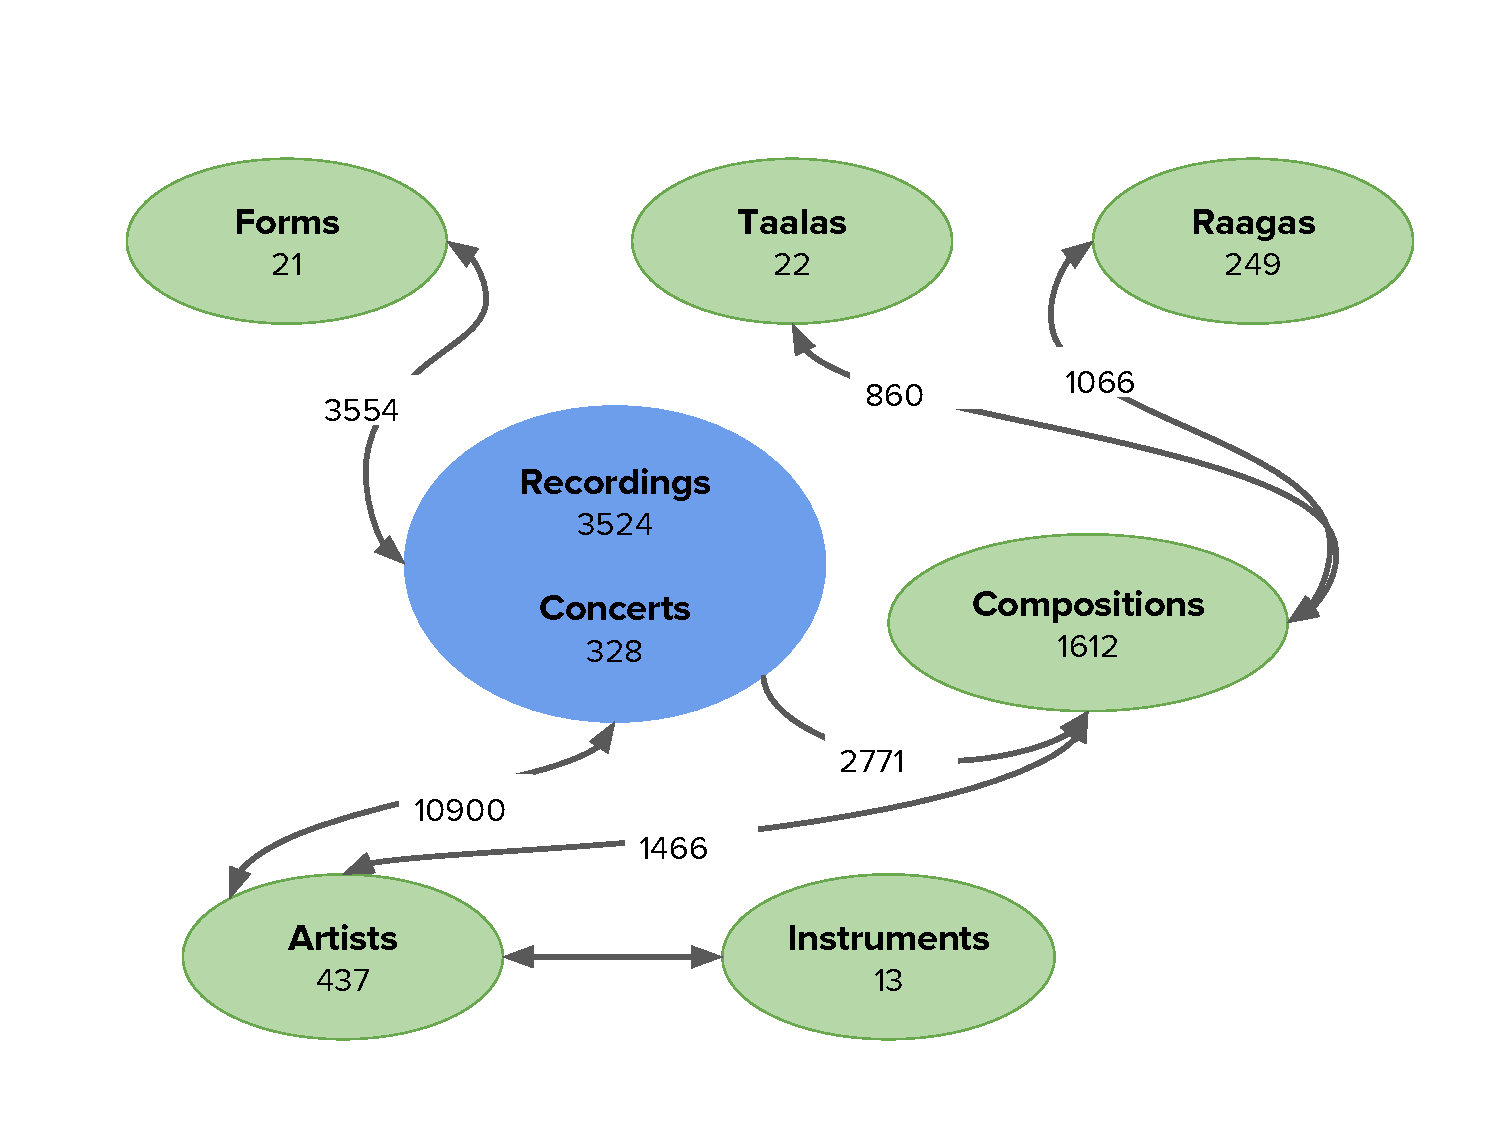
\includegraphics[width=\figSizeHundred]{ch04_datasets/figures/carnatic_corpus.pdf}
	\end{center}
	\caption{Details of the Carnatic music corpus in terms of the number of different musical entities and relationships between them.\TODO{redo fig}}
	\label{fig:carnatic_corpus_details}
\end{figure}

As mentioned, vocal music constitute a significant part of Carnatic music and it is largely based around compositions. Hence, lyrics play an important role in this music tradition. Scores on the other hand have a limited usability as the music is primarily improvisatory in nature. Nonetheless, for some computational analyses lyrics and scores might be useful, and hence, we make an effort to compile a small collection of them. For most of the currently performed compositions there exists several published compilations of lyrics and scores, for example the ones by the three most recognised composers; Tyagaraja~\citep{TKG_Rao_Tyagaraja}, Syama Sastri~\citep{TKG_Rao_syama} and Dikshitar~\citep{TKG_Rao_Muddusvami}. However, this data is not available in machine readable format and hence is not directly accessible for computational analysis. There are some good open repositories of lyrics such as sahityam.net\footnote{\url{http://sahityam.net/wiki/Main_Page}} that provide lyrics in machine readable format. Sahityam.net is considered as a wikipedia of lyrics of Carnatic music and is our primary source for lyrics. It currently hosts lyrics for about 1820 compositions of Carnatic music. Sources that provide music scores of Carnatic music in a machine readable format are scarce. A compilation of scores done by Dr.~Shivkumar Kalyanaraman\footnote{\url{http://www.shivkumar.org/}} is our main source of scores for Carnatic music.

In addition to the signal processing and machine learning based approaches, semantic analysis of \gls{iam} has been another topic of research in the CompMusic project. The music community and music concepts related information collected from various sources over the Internet comprise the input data to semantic anlaysis and is a part of the Carnatic music corpus. Kutcheries.com\footnote{\url{http://www.kutcheris.com/}} and Wikipedia\footnote{\url{https://en.wikipedia.org/wiki/Category:Carnatic_music}} are two sources utilized for obtaining such an information. Kutcheries.com is a good source of artist biographies and up-to-date information about music venues, concerts and other related events. The category of Carnatic music on Wikipedia is a good source of contextual information including music concepts. There has also been an effort to contribute to Wikipedia by adding information with the help of domain experts. In addition to these two sources, more opinion like data on different musical aspects is obtained from Rasikas.org\footnote{\url{http://www.rasikas.org}}, an active music forum dedicated to Carnatic music community. For the case of Carnatic music the data from rasikas.org can be considered as ideal for studying tasks such as community profiling.


\subsubsection{Coverage of Carnatic music Corpus}
\label{sec:corpus_coverage_of_carnatic_music_corpus}

Coverage analysis of a corpus aims to measure the representativeness and comprehensiveness of a corpus with respect to the reference sources that represent real-world collections. For the case of the Carnatic music corpus coverage analysis is performed for \glspl{raga}, \glspl{tala}, performing artists and composers. Kutcheris.com is our primary source for measuring artist coverage since it is up-to-date with current artists and their performances. We use last 5 years of their concert listing from 2009-2014. Release catalog from Charsur, our main reference as a record label also provides information about \glspl{raga}, \glspl{tala}, artists and composers. Raaga.com\footnote{\url{http://play.raaga.com/carnatic}}, an Indian music streaming service with a channel dedicated to Carnatic music is another source we considered for this analysis. It should be noted that Raaga.com has several light music forms included in their Carnatic music channel, which we have purposefully not included in our corpus. Hence, the numbers derived from an analysis done on the data from Raaga.com will have an adverse influence because of these additional music forms. The procedure followed for obtaining information from these sources and the post-processing done before the analysis is explained in the article by~\cite{CM_Corpora_Ajay14}.

For each music entity we define a coverage measure, the \textit{overlap} ($O$) as:

\begin{equation}
	O_{e}^{r} = \frac{ | S_{e}^{c} \cap S_{e}^{r} | }{ | S_{e}^{r} |}
	\label{eq:coverage_measure}
\end{equation}

\noindent where $O_{e}^{r}$ is the \textit{overlap} measure of the musical entity $e$ with respect to the reference source $r$, $S_{e}^{c}$ is the set of entities in the corpus and $S_{e}^{r}$ is the set of entities in the reference source. $|S|$ denotes the cardinality of a set $S$. In Table~\ref{tab:coverage_summary_carnatic_corpus} we summarize the coverage of the musical entities along with the overlap measure with respect to the reference sources mentioned above. We see that the coverage of the \glspl{raga} in the corpus is satisfactory and of the \glspl{tala} is good. For composers and artists the numbers are low when compared to Raaga.com, which can be attributed to the presence of light Carnatic music forms in their database. 

\begin{table}
\begin{centering}
\begin{tabular}{ c c c c c }
	\hline
					 & Corpus	& Raaga.com			& Kutcheris 	& Charsur\\
	\hline
	\Glspl{raga}	& 	246		& 	489 (42\%)		& 	N/A			& 301 (68\%)\\
	\Glspl{tala}	& 	18		& 	16 (100\%)		& 	N/A			& 21 (85\%)\\
	Composers		& 	131		& 	598 (17\%)		& 	N/A			& 256 (42\%)\\
	Artists			& 	233		& 	501				& 	2978		& 264 (48\%)\\						
	\hline
	
\end{tabular}
\par \end{centering}	
\caption[Coverage of the Carnatic music corpus]{Summary of the coverage of the Carnatic music corpus. The numbers in the paranthesis indicate the computed \textit{overlap} measure. N/A denotes data not available.} 
\label{tab:coverage_summary_carnatic_corpus}
\end{table}

Not all the performing artists in the corpus (\tabref{tab:coverage_summary_carnatic_corpus}) are lead artists. Among these 233 artists 74 are lead artists (lead vocal or lead instrumental), 28 are accompanying violinists and 48 are percussionists. Since Carnatic music corpus predominantly comprises vocal music, coverage of lead or vocal artists becomes more important. Also not every lead artist is equally popular, that should also be a consideration in measuring the representativeness of the corpus. The concerts listed by Kutcheris.com span the whole year and all through the day. However, the evening concerts are more
recognized, and we took that to be a measure of the popularity of an artist. For a better coverage analysis, we thus consider three categories of artists: Artists-Set-1 (all the artists), Artists-Set-2 (artists who have performed in the evening concerts, through the year) and Artists-Set-3 (artists who
have performed in evening concerts between November and January). Of the 2978 total artists present in Set-1 on Kutcheris.com concert listings, there are 1814 artists in Set-2 and 1472 artists in Set-3.

\begin{figure}
	\begin{center}
		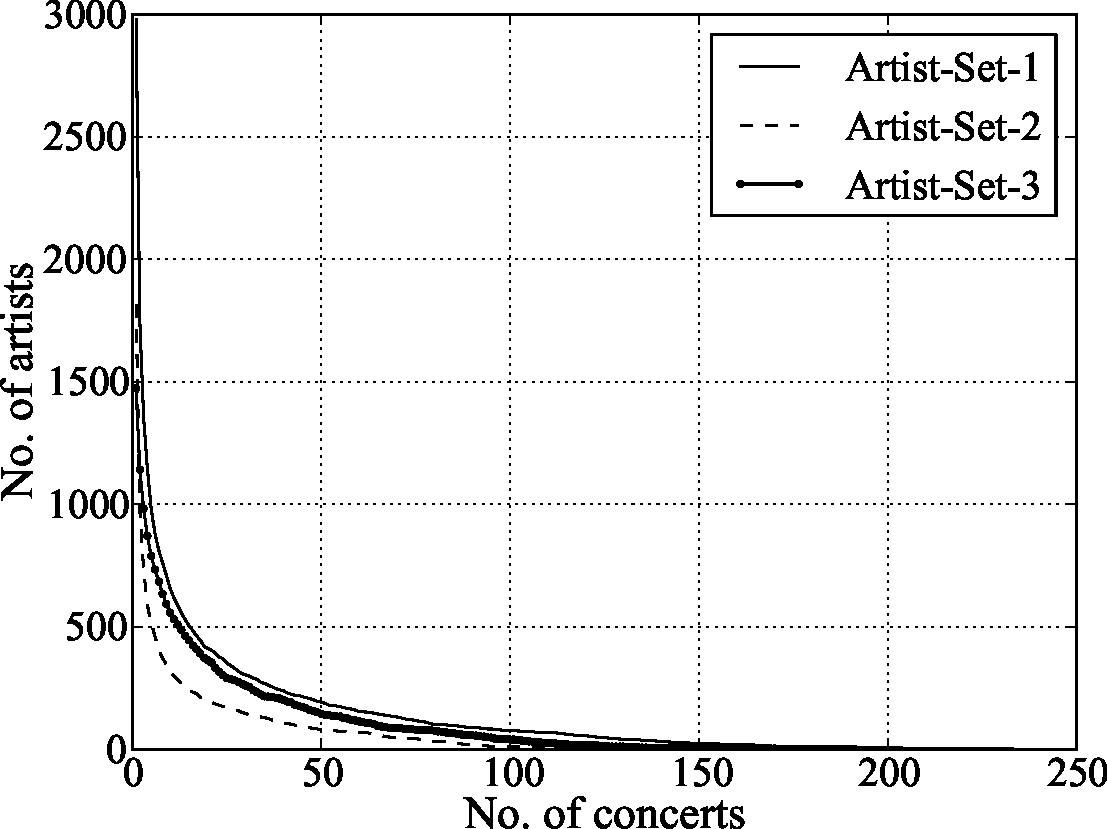
\includegraphics[width=\figSizeHundred]{ch04_datasets/figures/performances-vs-artists.pdf}
	\end{center}
	\caption{The number of artist by the number of their concerts. These artists are the ones obtained from Kutcheris.com}
	\label{fig:number_artrist_vs_number_concerts}
\end{figure}

In addition to the timing of the concerts, popularity of an artist can also be measured based on the number of concerts. Though there are a large number of artists listed in Kutcheris.com, we notice that the distribution of the number of concerts they have performed is exponential (\figref{fig:number_artrist_vs_number_concerts}). We see that there are only about 200 artists of 2978 artists who have performed in over 50 concerts. To consider this aspect while measuring coverage, we compute the \textit{overlap} as defined in \eqref{eq:coverage_measure} through different subsets of the artists in Kutcheris.com, sweeping over the number of concerts they have performed. Furthermore, we perform this analysis for different categories of the artists in the corpus as mentioned above.

\begin{figure}
	\begin{center}
		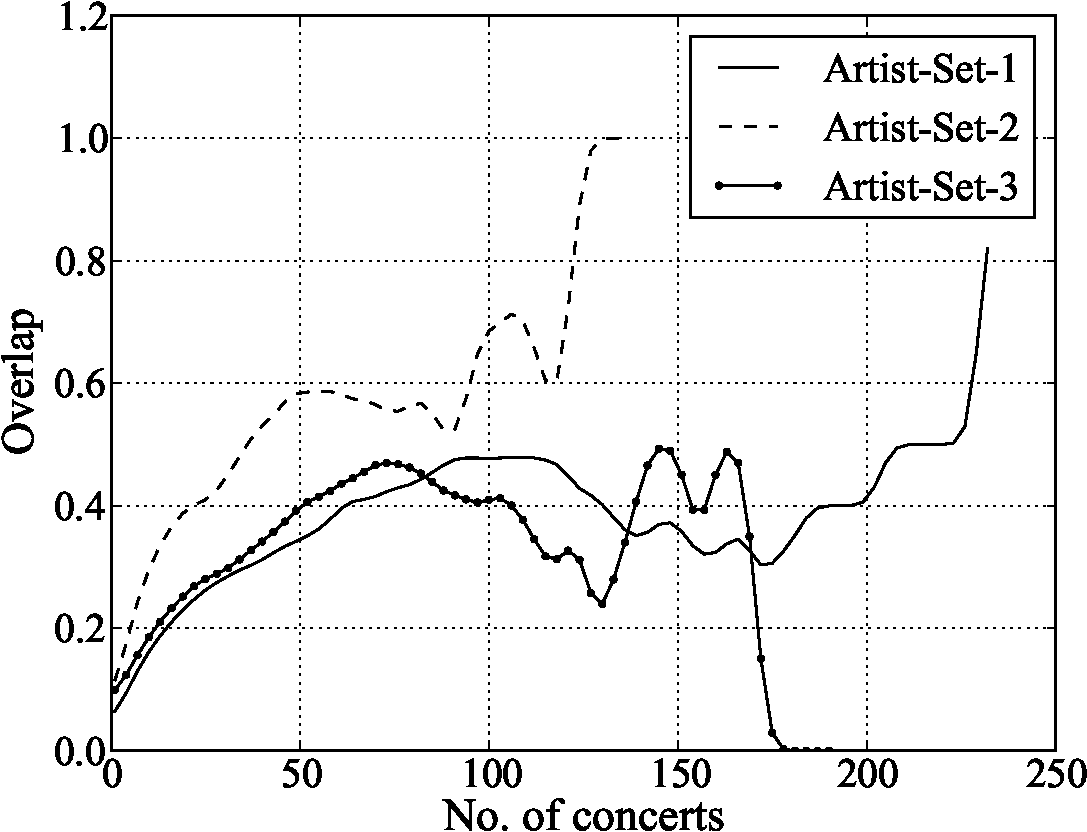
\includegraphics[width=\figSizeHundred]{ch04_datasets/figures/artist-coverage-vs-performances.pdf}
	\end{center}
	\caption{The \textit{overlap} between the artists in the corpus and those listed in Kutcheris.com for different artist sets determined by the number of performed concerts. The analysis is performed for every category of artists in the corpus.}
	\label{fig:artist_coverage_vs_number_of_concerts}
\end{figure}

In \figref{fig:artist_coverage_vs_number_of_concerts} we show the \textit{overlap} between the artists in the corpus and the ones listed in Kutcheris.com for different sets of artists based on the number of performed concerts. We compute the \textit{overlap} curve for all three categories of the artists in the corpus. We notice that the \textit{overlap} increases as we consider more frequently performing artists. We also observe that the \textit{overlap} saturates and becomes constant. This can be attributed to the fact that the most frequently performing artists are the accompanists and they are few in numbers compared to the lead artist, as they accompany multiple lead artists. Since the number of artists with more than 150 concerts is very less, the \textit{overlap}
values becomes unreliable. Overall we notice that the \textit{overlap} is better for artists in the category Artist-Set-2 than Artist-Set-1 and Artists-Set-3. This also indicates that the corpus has a better coverage of the artists from evening concerts round the year.


\subsubsection{Completeness of the Canatic Music Corpus}
\label{sec:corpus_completeness_of_completeness_of_carnatic_music_corpus}

As defined earlier, completeness of the corpus in the context of the CompMusic corpora refers mainly to the completeness of the associated metadata
for each recording. The editorial metadata as will be explained in detail (\secref{sec:corpus_storage_and_access}) is stored and accessed from MusicBrainz. There can be multiple reasons for missing and erroneous editorial metadata in the MusicBrainz. Many times commercially released CDs do not provide all the relevant editorial metadata on the cover-art. In several cases there is no mention of the accompanying artists or of the \gls{raga} and \gls{tala} of the musical piece. Very often composition information is missing on the CD cover. Another reason for incomplete metadata can be that the editorial metadata is not completely entered into the MusicBrainz. This happens quite frequently for the fields such as recording relationships. Several times the metadata entered is erroneous. This is either due to a mistake done by the person uploading the metadata into the MusicBrainz or that the editorial metadata provided on the CD cover itself is wrong. Multiplicity of languages used in Carnatic music further adds to these inconsistencies. There has been some effort to automatically complete the missing metadata based on the relationships on the release and the recordings using semantic web approaches. The missing metadata due to transliteration errors also has been addressed to an extent by making curated list of entities such as \gls{raga} and \gls{tala}, and using robust algorithm for matching and linking metadata. Despite these efforts, there are a significant number of recordings and releases for which the metadata is incomplete.


\begin{table}
	\begin{centering}
		\begin{tabular}{ c c c c}
			\hline
			Metadata	 		&  \#Recordings	& completeness (\%)\\
			\hline
			Lead artist			& 	1650	& 	100	\\						
			Accompanying artist	& 	1221	& 	74	\\
			\Glspl{raga}		& 	959		& 	58	\\
			\Glspl{tala}		& 	917		& 	56	\\
			Work (compositions)		& 	989		& 	60	\\
			
			\hline
			
		\end{tabular}
		\par \end{centering}	
	\caption[Completeness of the Carnatic music corpus]{Completeness of the Carnatic music corpus showing the number of recordings for which the corresponding metadata is available and the percentage (\%) of such recordings. The percentage values are rounded off to the nearest integer.} 
	\label{tab:completeness_carnatic_corpus}
\end{table}


In \tabref{tab:completeness_carnatic_corpus} we show the completeness of the recordings in the Carnatic music corpus. We see that all the recordings are at least labeled with a lead artist, but about a quarter of the recordings (429/1650) do not have any accompanying artist information. \Gls{raga}, \gls{tala} and work (composition) labels are available for more than half the number of recordings. Note that there are some recordings that have the required editorial metadata but deemed incomplete because the names could not be accurately matched to any entity in the curated list. 


\subsection{Hindustani Music Corpus}
\label{sec:corpus_hindustani_music_corpus}

Similar to the case of Carnatic music, \gls{raga} and \gls{tala} are the fundamental music concepts with which to describe melodic and rhythmic aspects of Hindustani music. They thus become the primary considerations while building the Hindustani music corpus as well. In Hindustani music also vocal music is predominant. However, compared to Carnatic music instrumental performances in Hindustani music are much more popular and prevalent. Hindustani music tradition as compared to Carnatic music is much more diverse and heterogeneous. One of the reasons for this can be the geographical spread of this music tradition. Hindustani music thus presents a significant challenge in compilation of a good research corpus. Another major difference between the two music traditions is that in Hindustani music the compositions are very short. The compositions basically act as base for improvisation, which is the main focus in a performance of Hindustani music. For compilation of the Hindustani music corpus we focus on two important vocal music styles; Dhrupad and Khy\={a}l (Section\TODO{Chapter ref}). %A Khy\={a}l performance typically has a lead vocals, a melodic accompaniment (typically given by harmonium or s\={a}ra\o{n}gi), a rhythm accompaniment (typically given by tabla) and a drone sound in the background (typically given by a t\={a}npura). 

There are many institutions that have compiled large audio archives of Hindustani music. The prominent ones among them are the \gls{itc-sra}, Sangeet Natak Academy, and the \gls{air}. Each of these institutions own thousands of hours of expert curated music recordings that represent the real world performance practices of Hindustani music. \gls{itc-sra} is a premier music academy of Hindustani music and has taken up major efforts in the archival of music. Sangeet Natak Academy is India’s national academy for music, drama and dance. \gls{air} is the largest public broadcaster in India and has a large archive of Hindustani music curated over many decades. \gls{air} awards grades to performing musicians and its archives can be considered as a reference for Hindustani music. Like in most of the cases, none of these archives is publicly available. In such a situation, we gathered commercially released audio recordings from several music labels and compiled our own corpus using these institutions as a reference. During this process we also consulted expert musicians and musicologists, such as Dr. Suvarnalata Rao at the \gls{ncpa}, Mumbai, India, to curate the audio collection in the corpus. 

The Hindustani music corpus primarily comprises khy\={a}l and dhrupad vocal music releases, though a significant number of instrumental music releases are also present. There are 233 releases with a total of 1096 recordings spanning over 300 hours of audio. The details of the Hindustani music corpus in terms of the unique number of recordings, releases, artists, \glspl{raga}, \glspl{tala} and compositions is shown in \figref{fig:hindustani_corpus_details}.


\begin{figure}
	\begin{center}
		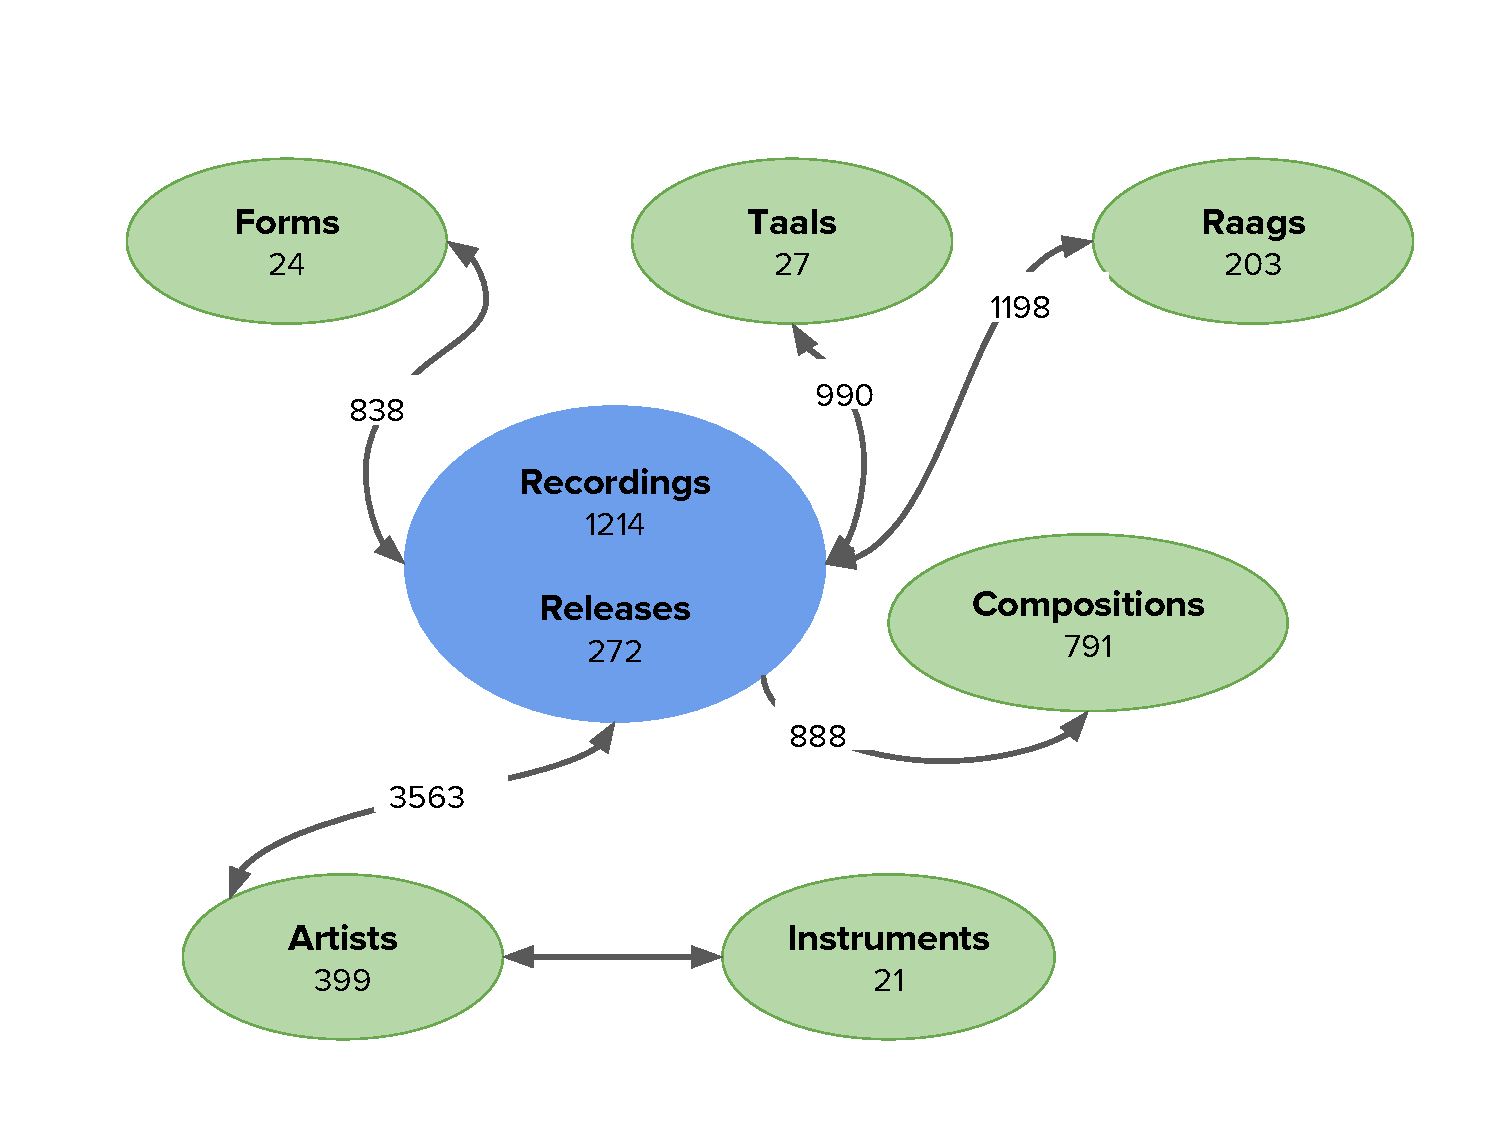
\includegraphics[width=\figSizeHundred]{ch04_datasets/figures/hindustani_corpus.pdf}
	\end{center}
	\caption[Details of the Hindustani music corpus]{Details of the Hindustani music corpus in terms of the number of different musical entities and relationships between them.\TODO{redo fig}}
	\label{fig:hindustani_corpus_details}
\end{figure}


As mentioned before, compositions in Hindustani music are short and they basically act as a base for improvisation. The music performances mainly comprise improvised music material. Due to these factors lyrics and scores are not very relevant for the computational anlaysis of Hindustani music. There exists few repositories such as Bhatkhande~\citep{Bhatkhande_1990} and Ramashray Jha~\citep{R_Jha_2001} who have compiled lyrics and scores of several bandishes (compositions) using a standard notation for Hindustani music. However, they are not available in a machine readable format. In addition to lyrics and scores there are some information repositories such as Swarganga Music Foundation\footnote{\url{https://www.swarganga.org/}} for musical concepts such as \glspl{raga}, \glspl{tala} and bandishes (compositions). The category of Hindustani music on Wikipedia\footnote{\url{https://en.wikipedia.org/wiki/Category:Hindustani_music}} is a good source of contextual information including music concepts of Hindustani music.

\subsubsection{Coverage of Hindustani Music Corpus}
\label{sec:corpus_coverage_of_hindustani_music_corpus}

For the coverage analysis of the Hindustani music corpus we follow exactly the same methodology as was for the Carnatic music corpus. The analysis is done for artists, \glspl{raga}, \glspl{tala} and compositions. Large geographical spread, lack of dedicated record labels and heterogeneous nature of the music make the coverage analysis of Hindustani music more complex compared to Carnatic music. Therefore, it is challenging to do a comprehensive artist coverage analysis like the one presented for Carnatic music. For each of the entities, we choose two main institutional references, \gls{itc-sra} and Swarganga. In  \tabref{tab:coverage_summary_hindustani_corpus} we show the coverage of the Hindustani music corpus. We see that even though the corpus and the chosen references have comparable the number of entities, the \textit{overlap} between them is less. This can be attributed to the differences in the purpose of creating the music collection. We mainly focused on recordings made in last 20-30 years to ensure good recording quality and to reflect current performance practices. On the other hand, both the references focus primarily on archiving Hindustani music and hence consist of several generations of artists, infrequent \glspl{raga} and \glspl{tala}, and a more comprehensive list of compositions. Furthermore, in our Hindustani music corpus we focus on vocal music recordings of only two styles, khy\={a}l and dhrupad. The reference archives additionally include instrumental music and several other styles of Hindustani music.


\begin{table}
	\begin{centering}
		\begin{tabular}{ c c c c}
			\hline
			& Corpus	& ITC-SRA			& Swarganga\\
			\hline
			Artists			& 	360		& 	240 (19\%)	& 	629 (14\%)\\						
			\Glspl{raga}	& 	176		& 	185 (48\%)	& 	534 (13\%)\\
			\Glspl{tala}	& 	32		& 	N/A			& 	59 (37\%)\\
			Works			& 	685		& 	N/A			& 	1957\\

			\hline
			
		\end{tabular}
		\par \end{centering}	
	\caption[Coverage of the Hindustani music corpus]{Coverage of the Hindustani music corpus. The numbers in the parenthesis indicate the computed \textit{overlap} measure. N/A denotes data not available.} 
	\label{tab:coverage_summary_hindustani_corpus}
\end{table}


\subsubsection{Completeness of Hindustani Music Corpus}
\label{sec:corpus_completeness_of_hindustani_music_corpus}

In \tabref{tab:completeness_hindustani_corpus} we show the completeness of the editorial metadata for Hindustani music. We see that the editorial metadata for all the recordings at least includes a lead artist, and for more than half of the collection, the accompanying artists. Roughly 90\% of the corpus is annotated with \gls{raga} label and more than half with \gls{tala} label. Work (bandish) labels are present for nearly half of the collection. \Gls{alap} performances in Hindustani music are completely improvisatory musical pieces and are not based on compositions. Also, they are unmetered in nature, and hence they are not assigned any \gls{tala} label. Ideally, such music pieces should be discounted while assessing the completeness of the work  and the \gls{tala} metadata. Due to unavailability of the \gls{alap} labels on recordings these performances are also included in the assessment and hence work and \gls{tala} completeness is an underestimate.



\begin{table}
\begin{centering}
	\begin{tabular}{ c c c c}
		\hline
		Metadata	 		&  \#Recordings	& completeness (\%)\\
		\hline
		Lead artist			& 	1096	& 	100	\\						
		Accompanying artist	& 	658		& 	60	\\
		\Glspl{raga}		& 	960		& 	88	\\
		\Glspl{tala}		& 	627		& 	57	\\
		Work (Bandish)		& 	576		& 	53	\\
		
		\hline
		
	\end{tabular}
	\par \end{centering}	
\caption[Completeness of the Hindustani music corpus]{Completeness of the Hindustani music corpus showing the number of recordings for which the corresponding metadata is available and the percentage (\%) of such recordings. The percentage values are rounded off to the nearest integer.} 
\label{tab:completeness_hindustani_corpus}
\end{table}


\subsection{Open-access Research Corpus}
\label{sec:corpus_open_access_research_corpus}

The audio recordings in both Hindustani and Carnatic music corpus are ripped from commercially released music CDs. The copyright on these recordings does not allow for a redistributed of the music content, and therefore, they cannot be made publicly available. Though these recordings are available in the market and are easily accessible, re-compiling the entire music corpus would practically require a lot of effort from a researcher who is trying to reproduce the research results. To promote the idea of open-access of research corpora and reproducibility of research results, in the CompMusic project there has been an effort to compile an open-access music collection. This open-access corpus comprises both Hindustani and Carnatic music. Like the other research corpora described in previous sections, this corpus contains audio recordings and associated editorial metadata. In addition, this corpus also contains several annotations of different music attributes such as melodic phrases, sama locations and sections. Due permissions are taken from the artists for redistribution of these audio recordings. As a result of which the corpus is made publicly available under creative commons license (CC BY-NC 4.0). The audio recordings in this corpus are hosted on Internet Archive\footnote{\url{https://archive.org/}} and made accessible through the Dunya Web \gls{api} (Section\TODO{secref}). 


\begin{figure}
	\begin{center}
		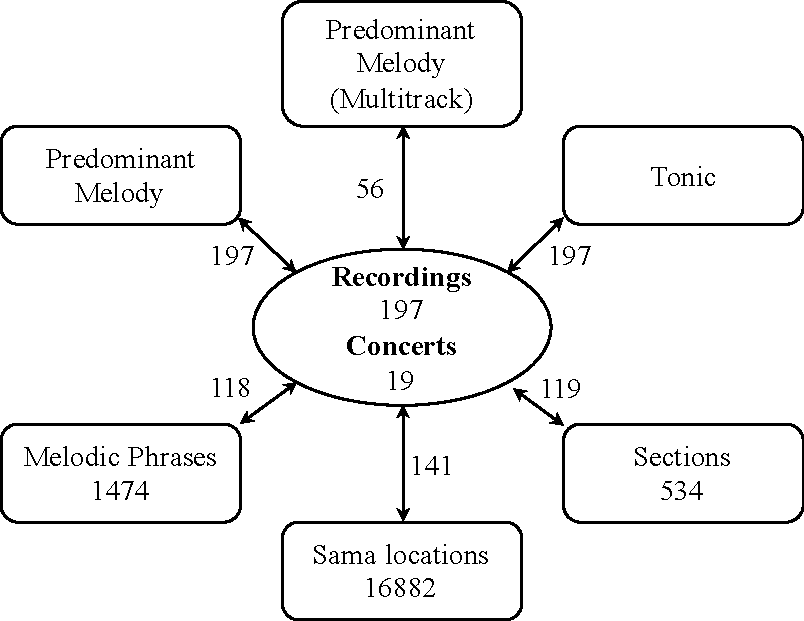
\includegraphics[width=\figSizeNinety]{ch04_datasets/figures/carnatic_CC_details.pdf}
	\end{center}
	\caption[Details of the Carnatic open-access music corpus]{Details of the Carnatic open-access music corpus in terms of the number of available annotations of different musical attributes and audio features.\TODO{redo fig}}
	\label{fig:carnatic_open_access_corpus_details}
\end{figure}

\TODO{details in terms of the different musical attributes, artist/forms/works etc? + Check the numbers of annotations, select only the releases which are there on the musicbrainz. We should now consolidate that collection}

The Carnatic music part of the open-access music corpus contains \TODO{XX} releases, \TODO{XX} number of recordings spanning \TODO{XX} hours of audio. A majority of these releases are recordings of Carnatic music concerts performed in the \gls{acc} in Chennai, India. These are multi-track recordings later mixed and mastered by a professional. Individual music pieces of a concert are split into separate recordings that then comprise a release. In addition to the content procured from the \gls{acc}, a number of releases in this corpus are commercially released CDs with artists' due permissions to make them publicly available. Along with the audio recordings and accompanying editorial metadata this corpus contains carefully done annotations corresponding to melodic, rhythmic and sectional aspects of the music. Manually done annotations include characteristic melodic phrases and sections within each audio recording. Semi-automatically done annotations include time-aligned sama locations and tempo in a recording. Finally, automatically done annotations, which can also be considered as mid-level audio features include predominant pitch contour and tonic frequency used in the recording by the lead artist. Since for several concerts their multi-track recordings are available, along with the predominant pitch estimated from the mix-down track we also compute pitch using the solo vocal track. These pitch contours from solo vocal tracks can serve as ground-truth data to evaluate pitch estimation algorithms for \gls{iam}. In \figref{fig:carnatic_open_access_corpus_details} we show the number of available annotations of different musical attributes and audio features for the Carnatic music part of the corpus.


\begin{figure}
	\begin{center}
		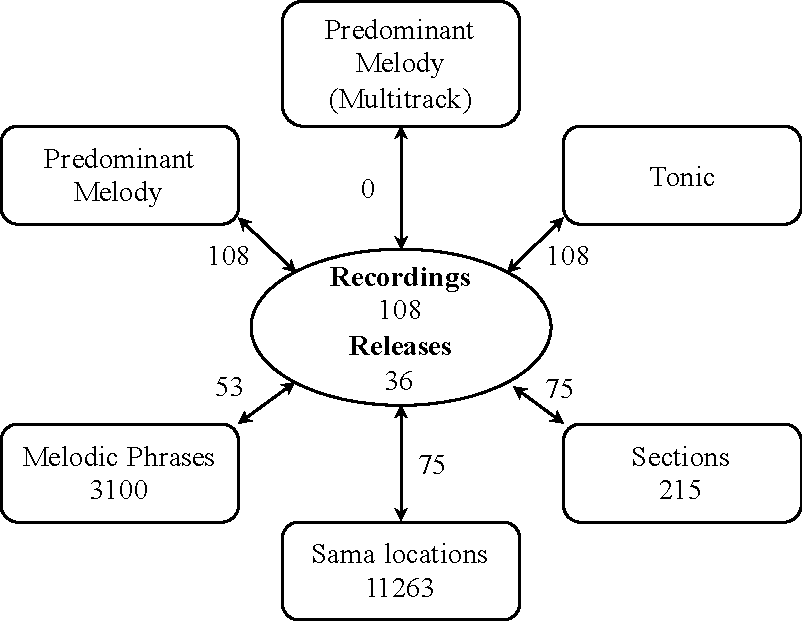
\includegraphics[width=\figSizeNinety]{ch04_datasets/figures/hindustani_CC_details.pdf}
	\end{center}
	\caption[Details of the Hindustani open-access music corpus]{Details of the Hindustani open-access music corpus in terms of the number of available annotations of different musical attributes and audio features.\TODO{redo fig}}
	\label{fig:hindustani_open_access_corpus_details}
\end{figure}

The Hindustani music part of the open-access music corpus contains \TODO{XX} releases, which has \TODO{XX} number of recordings spanning \TODO{XX} hours of music. A significant portion of this collection comprises commercial releases by maestros such as Pt.~Ajoy Chakbraborty and Pt.~Kumar Gandharva. The other portion of the collection comprises individual recordings procured from different professional musicians and grouped together into meaningful releases for each artist. The grouping is based on common performance practices clubbing the performances in the \glspl{raga} that are performed together in a concert. This corpus also contains annotations for characteristic melodic phrases, sections, time-aligned sama locations and tempo. It also contain mid-level audio features including predominant pitch contour and tonic frequency used in the recording. Since multi-track recordings are available for this collection, pitch contours extracted from solo vocal track are not present. In \figref{fig:hindustani_open_access_corpus_details} we show the number of available annotations of different musical attributes and audio features for the Hindustani music part of the corpus. 



\subsection{Storage and Access of Corpus}
\label{sec:corpus_storage_and_access}

The previous sections described  various aspects of the Carnatic and the Hindustani research music corpus compiled in the CompMusic project. In this section we provide details on how the data in the corpus is storage and ways to access the data.

The audio corresponding to the corpora described above are largely stereo recordings sampled at 44.1\,kHz. For a few performances in the Carnatic open-access music corpus multi-track recordings are available. Most of the audio recordings in the corpora are ripped from the commercially released CDs. These recordings are compressed and stored as 160\,kbps MP3 files. The audio recordings for the open-access music corpus are hosted on Internet Archive. The rest of the audio recordings are hosted on the servers in Universitat Pompeu Fabra. In addition to the audio data, the corpora contain different melody and rhythm related audio features such as predominant pitch contours, tonic and tempo value of the music recordings. These features are also hosted on the university servers along with the audio recordings.

As mentioned, for every single audio recording in the corpora there is an accompanying editorial metadata. The metadata typically includes the following fields; lead artist, accompanying artists, instrument played by these artists, \gls{raga} and \gls{tala} of the music piece, music form and the name of the composition. For the case of Hindustani music it also includes \gls{laya} information. All this metadata is stored in the MusicBrainz, an open music encyclopedia. Every music concept in the MusicBrainz has a unique identifier, which facilitates the processing of this metadata. A number of complexities and problems arising from different spellings of an entity or different aliases of an entity are well handled by using this schema. There are several other advantages of using the MusicBrainz repository for storing editorial metadata, such as its ability to publish its database into Linked Data\footnote{\url{http://linkeddata.org/}}, mapping of entity concepts to Music Ontology\footnote{\url{http://musicontology.com/}}, its \acrshort{rest}-based webservice \acrshort{api} for direct access to its data. Above all, its a community driven open-content initiative and has its majority of the data in public domain.

All the data associated with a recording; the audio file, extracted set of features and the accompanying metadata can be accessed through the Dunya platform\footnote{\url{http://dunya.compmusic.upf.edu/}}. Dunya exposes this data in two ways; through a web-based graphical interface and through a \acrshort{rest}-based \acrshort{api}. A detailed description of the Dunya platform and the ways to access the data is provided in Section\TODO{secref}. Note that though the data is accessible for research purposes after user registration, not all the data in the corpora is in public domain. \TODO{what more?}



\section{Test Datasets}
\label{sec:corpus_test_datasets}

As explained earlier, a test dataset is a subset of a corpus used for studying a specific task. Typically a dataset is specific to an experiment and may contain additional information such as annotations. We here present the datasets that are used in different studies as a part of this dissertation. These datasets can be used for evaluating computational approaches for different melodic analyses in \gls{iam}. Some of these datasets are quite generic and contain good quality comprehensive editorial metadata along with the audio recordings. And hence, we envision their usage in other melodic analysis tasks beyond the ones addressed in this dissertation.

Since a majority of these datasets are a subset of the corpora described in previous sections, details regarding the quality of audio recordings and editorial metadata remain the same as that of the corpora. In case of exceptions, these details are provided in the section where the dataset is described. 


\subsection{Tonic datasets}
\label{sec:corpus_tonic_datasets}


{\renewcommand{\arraystretch}{1.5}
\begin{sidewaystable} 
\begin{centering}
	\begin{tabular}{ c | c  c  c  c  c  c  c  c  c  c }
\tabletop
		Dataset 	&Avg. length (min)&\#Excerpts&	 	Hi.(\%) 	& 	Ca.(\%)	& 	Voc.
		(M/F)(\%) & Inst. (\%)	& 	\#Usong   	& 	\#Uartists	\\
\tablemid
		\acrshort{tds_cm1}		&3 &271	&	 41		& 	59	&	0			& 	100		& 	169		&	33	\\
		\acrshort{tds_cm2}		&3 &935	&	 45	 	& 	55	&	100 (68 / 32)		&	0		& 	547		&	81	\\
		\acrshort{tds_cm3}		&14.8&428	&	 45	 	& 	55	&	100 (72 / 28)		& 	0		&	428		&	71	\\
\hdashline
		\acrshort{tds_iitm1}		&144.6&38&	 0		& 	100	&	89 (79 / 21)		&	11		& 	N/A		&	22	\\
		\acrshort{tds_iitm2}		&12.3 &472	&	 0	 	& 	100	&	92 (77 / 23)		&	8		& 	472		&	22	\\
\hdashline
		\acrshort{tds_iisc}		&7.4&55	&	 0		& 	100	&	100 (80 / 20)		&	0		& 	55		&	5	\\
\tablebot
	\end{tabular}
	
	
	\caption[Summary of the tonic datasets]{Summary of the tonic datasets, including average excerpt length (Avg. length),
		number of excerpts (\#Excerpts), percentage of Hindustani music (Hi), Carnatic
		music (Ca), vocal excerpts (Voc.), instrumental excerpts (Inst.), number of
		unique songs (\#Usong) and number of unique artists (\#Uartists) in each dataset. For vocal
		excerpts we also provide the breakdown into male (M) and female (F)
		singers. Percentage (\%) values are rounded to the nearest integer.}
	\label{tab:tonic_datasets}
\par \end{centering}	
\end{sidewaystable}

We use six different datasets with varied characteristics for a comparative evaluation of approaches for tonic identification task in in \gls{iam}. The comparative evaluation is presented in \chapref{chap:data_preprocessing} and is based on our earlier work~\citep{Gulati2014Tonic}. Some of the tonic datasets overlap with the datasets used for evaluation in our earlier studies for the same task~\citep{salamon2012multipitch,gulati2012two}. A summary of the tonic datasets in terms of different attributes of the comprising excerpts such as their average length, their total number, proportion of Hindustani/Carnatic, instrumental/vocal and male/female excerpts, and unique number of songs and artists is provided in \tabref{tab:tonic_datasets}. In the subsequent paragraphs we describe each of these datasets in detail. Note that three out of the six datasets; \acrshort{tds_cm1}, \acrshort{tds_cm2} and \acrshort{tds_cm3} are compiled as a part of the work in this dissertation. 


\subsubsection{CompMusic Tonic Datasets}
\label{sec:corpus_compmusic_tonic_dataset}

The first three datasets shown in \tabref{tab:tonic_datasets}; \acrshort{tds_cm1}, \acrshort{tds_cm2} and \acrshort{tds_cm3} are tonic datasets compiled as a part of the CompMusic project. They are derived from the Carnatic and the Hindustani research corpus described in the previous sections. These datasets contain audio excerpts, associated metadata (lead artist, lead instrument, gender of the lead artist in case of a vocal performance) and tonic frequency annotation for every audio recording. The main differences across these three datasets are in terms of the duration of the excerpts and the type of music performance (vocal vs instrumental). These datasets comprise a diverse set of artists and music material such as gender of the singer, set of \glspl{raga} and music forms. Due to the diversity present in the datasets and the fact that these excerpts are taken from commercial releases, they can be regarded as a representative collection of \gls{iam} performances for tonic identification.  

\acrshort{tds_cm1} and \acrshort{tds_cm2} comprise three minute long audio excerpts extracted from full length recordings in the Hindustani and Carnatic music corpus. If a recording is longer than 12\,minutes, we extracted 3 excerpts from the beginning, middle and end of the recording. If the recording was shorter than 12\,minutes only one excerpt from the beginning was extracted. By taking excerpts from different sections of a song we ensure that the datasets are representative, since the musical characteristics can change significantly between different parts of a recording. \acrshort{tds_cm1} contains exclusively instrumental performances, and does not overlap with \acrshort{tds_cm2} and \acrshort{tds_cm3}. The latter two contain exclusively vocal performances, where \acrshort{tds_cm3} contains full performances and \acrshort{tds_cm2} contains excerpts taken from these performances. 

The tonic pitch for the vocal performances and tonic pitch-class for the instrumental performances was manually annotated for each excerpt. All the annotations were later verified by a professional Carnatic musician and the number of discrepancies was very small and later corrected. To assist the annotation process, we used the tonic candidate generation part of the approach proposed by \cite{salamon2012multipitch}. For every excerpt the top 10 tonic candidates were synthesized and played together with the original audio file to help identify and label the correct candidate. Note that the correct tonic pitch was always present amongst the top 10 candidates. A detailed description of this procedure is provided in~\cite{SGulati_MThesis2012}.


\TODO{A figure of tonic values in 428 + 169 performances}

\subsubsection{IITM Tonic Datasets}
\label{sec:corpus_iitm_tonic_datasets}

Datasets \acrshort{tds_iitm1} amd \acrshort{tds_iitm2} summarized in \tabref{tab:tonic_datasets} are compiled by~\cite{bellur2012knowledge}. These datasets were compiled by selecting 40 concerts from a private collection of hundreds of live concert recordings. These 40 concerts comprise 472 music pieces of Carnatic music. In order to study the robustness of tonic identification methods, the concerts that were selected range from artists from the 1960's to present day artists. The quality of the recordings vary from poor to good, usually depending on the period in which they were made. \acrshort{tds_iitm1} comprises 38 of these full-length concerts. \acrshort{tds_iitm2} comprises full length music pieces extracted from the 40 selected concert recordings. These performances are of varying duration, ranging from 46 seconds to 85 minutes. The tonic pitch for \acrshort{tds_iitm1} amd \acrshort{tds_iitm1} was manually annotated by a professional Carnatic musician.


\subsubsection{IISC Tonic Dataset}
\label{sec:corpus_iisc_tonic_dataset}

Dataset \acrshort{tds_iisc} is compiled by~\cite{ranjani2011carnatic}. It comprises audio recordings obtained from an online Carnatic music archive\footnote{\url{http://www.shivkumar.org/music/index.html}}. The archive is compiled by Carnatic musician and enthusiast Dr.~Shivkumar Kalyanaraman for the benefit of music amateurs and hobbyists as an online educational resource. The archive includes various forms of Carnatic music. \acrshort{tds_iisc} consists of 55 music pieces in the \gls{alapna} form, recorded by five singers across seven \glspl{raga}. The total duration of the dataset is 6.75\,hours. It includes recordings from the last 50 years, many of which were recorded live on analog audio tapes. The overall quality of the recordings is not very high. This makes it a challenging dataset for evaluating the accuracy of tonic identification approaches. The tonic pitch for recordings in this dataset was manually annotated by two professional musicians, S.~Raman and S.~Vijayalakshmi.


These six datasets represent the diversities present in real-world music collections of \gls{iam} in terms of the audio quality and music material, with which one can study the task of automatic tonic identification. To the best of our knowledge these are the largest and the most comprehensive datasets available for studying the task of tonic identification in \gls{iam}. \TODO{How can we obtain this dataset}



\subsection{Nyas dataset}
\label{sec:corpus_nyas_dataset}

\Gls{nyas} dataset~(\acrshort{nds_cm}) is used for evaluating our proposed approach (described in \chapref{chap:data_preprocessing}) to identify \gls{nyas} \gls{svara} segments in melodies of \gls{iam}. \acrshort{nds_cm} comprises 20 audio music recordings of total duration of 1.5\,hours. All of these recordings are of vocal \gls{alap} performances of Hindustani music. \Gls{alap} is unmetered melodic improvisational, usually performed at the opening of a \gls{raga} rendition. We selected only \gls{alap} performances because the concept of \gls{nyas} is emphasized in these sections during a \gls{raga} rendition. Of the 20 audio recordings, 15 are polyphonic commercially available recordings taken from the Hindustani music research corpus (\secref{sec:corpus_hindustani_music_corpus}). The other 5 audio recordings in the data set are monophonic in-house studio recordings of the \glspl{alap} sung by a professional singer of Hindustani music. These in-house recordings are available under Creative Commons (CC) license in Freesound\footnote{http://www.freesound.org/people/sankalp/packs/12292/}. In total we have performances by 8 artists in 16 different \glspl{raga}. To avoid over-fitting of the data it is important to include different artists and \glspl{raga} as the \gls{nyas} characteristics highly depend on these aspects~\cite{Dey2008}.

\Gls{nyas} segments were annotated by a performing artist of Hindustani music (vocalist) who has received over 15 years of formal musical training. The musician marked all the \gls{nyas} segment boundaries and labeled them appropriately. This dataset contains 1257 \gls{nyas} \gls{svara} segments. The duration of these segments vary from 150\,ms to 16.7\,s with a mean of 2.46\,s and median of 1.47\,s.


%%Things to include in description
%1) What is the dataset for (which problem)
%2) Where is the problem addressed in this thesis. Which paper have we used this dataset in
%3) What are the other studies in which this is used
%4) Who compiled the dataset
%5) What does the dataset constitute (audio, metadata and what annotations)
%6) What is the musical characteristics of this data (vocal/instrumental, number of artists, number of songs, number of compositions, audio quality, music tradition, music forms)
%7) Possible table of different attributes of annotated data (length, stats etc)
%7) Annotation procedure followed

\subsection{Melodic Similarity Dataset}
\label{sec:corpus_melodic_similarity_dataset}

Melodic similarity dataset~(\acrshort{msds}) is built for evaluating approaches for computing similarity between short melodic fragments in \gls{iam}. Since the melodic characteristics across Carnatic and Hindustani music differ considerably, it is preferred to perform evaluations on each music tradition separately. Therefore, this dataset is divided into two parts; Carnatic music melodic similarity dataset (\acrshort{msds_iitm_cmd}) and Hindustani music melodic similarity dataset (\acrshort{msds_iitb_hmd}). Both these datasets contain audio recordings, bare minimum metadata (lead singer and \gls{raga} label for each recording) and time-aligned annotations of characteristic melodic phrases. \acrshort{msds_iitb_hmd} also contains predominant pitch estimated using a semi-automatic approach proposed by~\cite{rao2010vocal,rao2009applications}. \acrshort{msds_iitm_cmd} is compiled at DONLab in Indian Institute of Technology Madras, Chennai, India. This dataset was introduced by~\cite{Ishwar2013}, and since then it has undergone several changes. \acrshort{msds_iitb_hmd} is compiled at Digital Audio Processing Lab in Indian Institute of Technology Bombay, Mumbai, India. This dataset was introduced by~\cite{Ross2012b}, and has also undergone changes since then. Both these datasets have been used in several studies for a similar task~\cite{Ishwar2013, Ross2012b, Rao2014}\TODO{confirm if it was the same dataset used in other paper from IITB and IITM}.  We describe and share the version of these datasets used for the experiments done as a part of this dissertation (\TODO{chapter ref}), which are originally presented in~\cite{gulati_ICASSP2015,gulati_ISMIR_2015}.

\acrshort{msds_iitm_cmd} and \acrshort{msds_iitb_hmd} comprise polyphonic vocal music recordings of renowned artists in both Carnatic and Hindustani music. In \tabref{tab:melodic_similarity_dataset_details} we summarize the relevant details for both the datasets.  We see that these datasets are diverse in terms of the number of artists. 

{\renewcommand{\arraystretch}{1.5}
\begin{table} 
	\begin{centering}
		\begin{tabular}{ c | c c c c c}
\tabletop
			Dataset   	& 	Rec. 	&	PT		&	R\={a}gs	&	Artists		&	Duration\,(hr)\\	
\tablemid
			\acrshort{msds_iitm_cmd}   	& 	23 	&	5		&	5 	&	14		&	3.82\\	
			
			\acrshort{msds_iitb_hmd}   	& 	10 	&	5		&	2	&	8		&	1.92\\	
\tablebot
		\end{tabular}
		\caption[Details of the melodic similarity datasets]{Details of the melodic similarity datasets in terms of the total number of recordings~(Rec.), number of annotated pattern types~(PT), number of r\={a}gs, unique number of artists and total duration of the dataset.}
		\label{tab:melodic_similarity_dataset_details}
	\par \end{centering}
\end{table}

The melodic phrases in \acrshort{msds} are annotated by two professional musicians (one for each music tradition) who have received over 15 years of formal music training. All the annotated phrases are the characteristic melodic phrases of the \glspl{raga}. These characteristic melodic phrases are distinctly recognized by musicians, due to this fact the ambiguity involved in the judgment of melodic similarity is minimized to an extent. For both the datasets occurrences of five different melodic phrases are annotated. In \tabref{tab:categorywise_details_melodic_similarity_dataset} we summarize the relevant details for every category of the annotated melodic phrases for both the datasets. From the table we get an idea about the length of these phrases across their occurrences for each phrase type. In general, we see that the phrases in Hindustani music as compared to Carnatic music have a higher degree of variation in terms of their length. 

{\renewcommand{\arraystretch}{1.5}
\begin{table} 
	\begin{centering}
		\begin{tabular}{ c c|c c c c c c}
\tabletop
			Dataset	& PT 	&	\#Occ & $L_{\mathrm{mean}}$ & $L_{\mathrm{std}}$ &	$L_{\mathrm{median}}$ & $L_{\mathrm{min}}$ 	&	$L_{\mathrm{max}}$\\
\tablemid
		 \multirow{5}{*}{\acrshort{msds_iitm_cmd}} 
		
		 & $C_1$ & 31	&	1.41 & 0.24 &	1.44 &	0.99 	&	1.94	\\ 
		 & $C_2$ & 33	&	1.28 & 0.21 &	1.26 &	0.91 	&	1.91\\
		 & $C_3$ & 32	&	1.22 & 0.25 &	1.15 &	0.74 	&	1.71\\
		 & $C_4$ & 26	&	1.12 & 0.17 &	1.06 &	0.9 	&	1.6\\
		 & $C_5$ 	& 35&	0.75 & 0.09 &	0.74 &	0.63 	&	0.98\\
\tablemid
		 Overall	&  	& 157&	1.15 & 0.31 &	1.12 &	0.63 	&	1.94\\
\tabletop		 
		 \multirow{5}{*}{\acrshort{msds_iitb_hmd}} 
		 &  $H_1$ & 41	&	1.80 & 1.06 &	1.44 &	0.73 	&	5.26	\\ 
		 & $H_2$ & 139	&	1.33 & 0.74 &	1.22 &	0.38 	&	5.23 \\
		 & $H_3$ & 21	&	1.24 & 0.62 &	1.16 &	0.53 	&	2.82\\
		 & $H_4$ & 61	&	2.25 & 1.30 &	1.74 &	0.51 	&	5.93\\
		 & $H_5$ & 78	&	1.15 & 0.32 &	1.13 &	0.416 	&	2.64\\
\tablemid
		 Overall	&  	& 340 &	1.51 & 0.92 &	1.23 &	0.38 	&	5.93\\
 
					
\tablebot
		\end{tabular}
		\caption[Details of the annotated characteristic melodic patterns in \acrshort{msds} dataset.]{Details of the annotated characteristic melodic patterns in \acrshort{msds} dataset. PT:~phrase type, \#Occ:~number of annotated occurrences of  patterns of a PT, and $L_{\mathrm{mean}}$, $L_{\mathrm{std}}$, $L_{\mathrm{median}}$, $L_{\mathrm{min}}$ and $L_{\mathrm{max}}$ are the mean, standard deviation, median, minimum and maximum value of the lengths of the phrases of a PT.} 
		\label{tab:categorywise_details_melodic_similarity_dataset}
	\par \end{centering}
\end{table}

To correctly evaluate a method for an information retrieval task, it is important that the ground-truth annotations are complete, meaning that they cover all the occurrences of an object that the method aims to retrieve. Failing to do so might degrade the precision measurement of the method. In our case, wherein we evaluate the task of melodic similarity by casting it as a retrieval task, a similar situation exists. Along with the size of the dataset in terms of the number of melodic phrases, it is important that these annotations cover all occurrences of a melodic phrase. In \acrshort{msds} we discovered a number of discrepancies where several occurrences of the melodic phrases considered in this dataset were not annotated. When these cases were shown to musicians who annotated the dataset, they were surprised to know the errors in their annotations. Both the musicians commented that the possible reason why they missed marking such phrases was the melodic context in which these phrases are sung. When these phrases are played in isolation (without any melodic context) they appear to belong to the phrase categories considered in \acrshort{msds}. However, when played with the melodic context (i.e. including audio from a few seconds before the onset of the phrase) masks their identity and their identification becomes harder. Many such missed occurrences of the melodic phrases were added to \acrshort{msds} to build a revised version of the dataset, which we denote by \acrshort{msds_cm}. \acrshort{msds_cm} comprises exactly the same set of audio recordings as \acrshort{msds}. The only difference is in terms of the occurrences of the melodic phrases. In  \tabref{tab:categorywise_details_revised_melodic_similarity_dataset} we summarize the relevant details for every category of the annotated melodic phrases in both the datasets in \acrshort{msds_cm}. Comparing \tabref{tab:categorywise_details_melodic_similarity_dataset} and \tabref{tab:categorywise_details_revised_melodic_similarity_dataset} we notice that in the new dataset nearly 25\% of the melodic phrases are added. Note that the added annotations of the melodic phrases are verified by the same musicians who originally annotated the datasets.


{\renewcommand{\arraystretch}{1.5}
	\begin{table} 
		\begin{centering}
			\begin{tabular}{ c c|c c c c c c}
				\tabletop
				Dataset	& PT 	&	\#Occ & $L_{\mathrm{mean}}$ & $L_{\mathrm{std}}$ &	$L_{\mathrm{median}}$ & $L_{\mathrm{min}}$ 	&	$L_{\mathrm{max}}$\\
				\tablemid
				\multirow{5}{*}{\acrshort{msds_cm_cmd}} 
				& $C_1$ & 39 & 1.38 & 0.25 & 1.35 & 0.87 & 1.94\\
				& $C_2$ & 46 & 1.25 & 0.21 & 1.25 & 0.81 & 1.9\\
				& $C_3$ & 38 & 1.23 & 0.24 & 1.16 & 0.74 & 1.7\\
				& $C_4$ & 31 & 1.1  & 0.17 & 1.07 & 0.8  & 1.61\\
				& $C_5$ & 45 & 0.76 & 0.08 & 0.76 & 0.62 & 0.98\\
				\tablemid
				Overall	&  	& 199& 1.14 & 0.3  & 1.12 & 0.63 & 1.94\\
				
				\tabletop		 
				\multirow{5}{*}{\acrshort{msds_cm_hmd}} 
				&  $H_1$& 62	&	1.93 & 0.98	&	1.61 &	0.73	&	4.52\TODO{WHY LESS??}\\
				& $H_2$ & 154 	& 	1.4  & 0.8 	& 	1.22 & 	0.38 	& 5.23 \\
				& $H_3$ & 47  	& 	1.3  & 0.8 	& 	1.08 & 	0.53 	& 4.49\\
				& $H_4$ & 76  	& 	2.38 & 1.34	& 	1.89 &	0.5  	& 5.93\\
				& $H_5$ & 87  	& 	1.17 & 0.37	& 	1.14 & 	0.42 	& 2.64\\
				
				\tablemid
				Overall	&  	& 426 & 1.6 & 0.99& 1.27 & 0.38 & 5.93\\
				
				\tablebot
			\end{tabular}
			\caption[Details of the annotated characteristic melodic patterns in \acrshort{msds_cm} dataset.]{Details of the annotated characteristic melodic patterns in \acrshort{msds_cm} dataset. PT:~phrase type, \#Occ:~number of annotated occurrences of  patterns of a PT, and $L_{\mathrm{mean}}$, $L_{\mathrm{std}}$, $L_{\mathrm{median}}$, $L_{\mathrm{min}}$ and $L_{\mathrm{max}}$ are the mean, standard deviation, median, minimum and maximum value of the lengths of the phrases of a PT.} 
			\label{tab:categorywise_details_revised_melodic_similarity_dataset}
			\par \end{centering}
	\end{table}
		
\subsection{\titlecap{\glsentrytext{raga}} Recognition Datasets}
\label{sec:corpus_raga_recognition_datasets}

As mentioned before, there are considerable differences in the melodic characteristics of Carnatic and Hindustani music. We therefore consider two separate datasets for evaluating approaches proposed for automatic \gls{raga} recognition~\TODO{Chapter ref}. Carnatic music \gls{raga} recognition dataset (\acrshort{rrds_cmd_big}) is a subset of Carnatic music research corpus (\secref{sec:corpus_carnatic_music_corpus}) and is built as a part of the work done for this dissertation. \acrshort{rrds_cmd_big} was introduced in~\cite{gulatiphrase_2016}. \acrshort{rrds_cmd_big} comprises 124\,hours of audio recordings and editorial metadata that includes carefully curated and verified \gls{raga} labels. \acrshort{rrds_cmd_big} contains 480 recordings belonging to 40 \glspl{raga} with 12 recordings per \gls{raga}. This dataset primarily consists of vocal performances of 62 different artists. There are a total of 310 different compositions belonging to diverse forms in Carnatic music (for example k\={i}rtana, varnam, virtuttam). The chosen \glspl{raga} contain diverse set of \glspl{svara} (note), both in terms of the number of \glspl{svara} and their pitch-classes (svarasth\={a}n\={a}s). Several selected \glspl{raga} share a common set of notes. This increases the complexity of the task, since the discrimination between these \glspl{raga} is mainly based on the temporal aspects of melody such as phrases and calan (Section\TODO{secref for calan}). To have diversity in the dataset we selected both phrase-based and scale-based \glspl{raga}. In order to simulate the effect of small number of \glspl{raga} present in an evaluation dataset we also consider a subset of this dataset, denoted by \acrshort{rrds_cmd_small}. It contains 120 recordings belonging to 10 \glspl{raga}. \TODO{dataset detail, stats of the dataset + per raga stats and names of raga and svaras}

Hindustani music \gls{raga} recognition dataset (\acrshort{rrds_hmd_big}) is a subset of Hindustani music research corpus (\secref{sec:corpus_hindustani_music_corpus}) built as a part of the work done for this dissertation. \acrshort{rrds_hmd_big} was first introduced in~\cite{gulati_tdms_2016}. \acrshort{rrds_hmd_big} comprises nearly 130\, hours of audio recordings and editorial metadata. \acrshort{rrds_hmd_big} contains full-length recordings of 300~Hindustani music performances belonging to 30~\glspl{raga} with 10~music pieces per \gls{raga}. The selected music material is diverse in terms of the number of artists, the number of forms, and the number of compositions. \TODO{dataset detail, stats of the dataset + per raga stats and names of raga and svaras}

\acrshort{rrds_cmd_big} and \acrshort{rrds_hmd_big} can be regarded as representative subsets of real-world collections of \gls{iam}. To the best of our knowledge these are the largest and the most comprehensive (in terms of the available metadata) datasets available for studying the task of automatic \gls{raga} recognition. \TODO{How can we obtain these datasets}











%\cleartorecto%!TEX root = ../thesis_a4.tex

\chapter{Melody Descriptors and Representations}
\label{chap:data_preprocessing}

\section{Introduction}
\label{sec:data_preprocessing_intro}

In this chapter, we describe methods for extracting relevant melodic descriptors and low-level melody representation from raw audio signals.  These melodic features are used as inputs to perform higher level melodic analysis by the methods described in the subsequent chapters. Since these features are used in a number of computational tasks, we consolidate and present these common processing blocks in the current chapter. This chapter is largely based on our published work presented in~\cite{Gulati2014Tonic,gulati2014Landmark,gulati_SITIS_2014}.

There are four sections in this chapter, and in each section, we describe the extraction of a different melodic descriptor or a representation.
\begin{itemize}
	\item In \secref{sec:data_preprocessing_tonic_identification}, we focus on the task of automatically identifying the tonic pitch in an audio recording. Our main objective is to perform a comparative evaluation of different existing methods and select the best method to be used in our work.
	\item In \secref{sec:data_preprocessing_melody_processing}, we present the method used to extract the predominant pitch from audio signals, and describe the post-processing steps to reduce frequently occurring errors.
	\item In \secref{sec:pre_processing_nyas_segmentation}, we describe our \gls{nyas}-based approach for segmenting melodies in Hindustani music. 
	\item In \secref{sec:pre_processing_tani_segmentation}, we describe the process of segmenting the solo percussion regions (\Gls{tani} sections) in the audio recordings of Carnatic music.  
\end{itemize}
	
%Along with the description of these method we also provide relevant implementation details and their default parameter settings. 

\section{Tonic Identification: Approaches and Comparative Evaluation}
\label{sec:data_preprocessing_tonic_identification}

The tonic pitch of a lead artist in \gls{iam} is the base frequency that serves as a reference and foundation for melodic integration throughout the performance. All the tones in the musical progression are always in reference and related to the tonic pitch (\secref{sec:melody_in_iam}). Therefore, for a meaningful comparison of melodies across recordings, it is important that the melodic representation is normalized by the tonic pitch in the recording. Identification of the tonic pitch in an audio recording thus becomes a crucial first step in melodic analysis of \gls{iam}. 

There exist a number of approaches for identifying tonic pitch in an audio recording of \gls{iam}~\citep{salamon2012multipitch,gulati2012two,bellur2012knowledge,ranjani2011carnatic,Sengupta2005b,chordia2013joint}. We present a detailed review of these approaches in \secref{sec:background_relevant_work_tonic_identification}. In our previous studies on tonic identification we showed promising results with identification accuracies close to 90\%~\citep{salamon2012multipitch,gulati2012two}. Similar accuracies are reported in other studies~\citep{ranjani2011carnatic,bellur2012knowledge}. As seen in our review (\secref{sec:background_relevant_work_tonic_identification}), it is misleading to draw a consensus on the best performing method just based on the accuracy reported in the publications. It is because these approaches are evaluated using different datasets with varied musical characteristics and under different experimental setup. 

In order to identify the most reliable, robust, and scalable approach, we perform their comparative evaluation using the same music collection and the same experimental setup. For this, we use a number of sizable datasets with varied musical and acoustical characteristics that are representative of the audio collections in \gls{iam}. In the subsequent sections, we describe the comparative evaluation, which is based on our earlier work presented in~\cite{Gulati2014Tonic}. The experimental setup and the datasets used for the evaluation are described in~\secref{sec:pre_processing_experimental_setup}. A detailed discussion of the results of the evaluation along with an in depth error analysis is presented in~\secref{sec:pre_processing_tonic_identification_results}. We then explain a heuristic-based majority voting process to correct the frequently occurring errors in tonic identification~(\secref{sec:pre_processing_tonic_identification_correcting_errors}). 


\subsection{Comparative Evaluation Setup}
\label{sec:pre_processing_experimental_setup}

We evaluate seven of the nine tonic identification methods listed in \tabref{tab:pre_processing_tonic_identification_summary_methods}. The methods selected for evaluation are
denoted by \acrshort{tonicid_justin}~\citep{salamon2012multipitch}, \acrshort{tonicid_sankalp}~\citep{gulati2012two}, \acrshort{tonicid_ranjani_1} and \acrshort{tonicid_ranjani_2}~\citep{ranjani2011carnatic}, \acrshort{tonicid_ashwin_1}, \acrshort{tonicid_ashwin_2} and \acrshort{tonicid_ashwin_3}~\citep{bellur2012knowledge}. Note that \acrshort{tonicid_sengupta}~\citep{Sengupta2005b} was not available for
evaluation and \acrshort{tonicid_chordia}~\citep{chordia2013joint} was not available when the experiments were conducted. 

Each of the method mentioned above is evaluated using six different datasets, \acrshort{tds_cm1}, \acrshort{tds_cm2}, \acrshort{tds_cm3}, \acrshort{tds_iitm1}, \acrshort{tds_iitm2} and \acrshort{tds_iisc}. A detailed description of these datasets in terms the musical material and the audio quality is given in~\secref{sec:corpus_tonic_datasets}. A summary of the datasets can be obtained from~\tabref{tab:tonic_datasets}. The diversities present in \gls{iam} repertoire in terms of the musical and acoustical characteristics are well captured in these six datasets. Note that \acrshort{tonicid_ashwin_1} method requires several excerpts from the same concert as an input, which is only available in the case of \acrshort{tds_iitm1} dataset. Hence, \acrshort{tonicid_ashwin_1} is only evaluated using \acrshort{tds_iitm1} dataset.

For vocal performances, we evaluate the accuracy of correctly identifying the tonic pitch, whereas, for instrumental music, we evaluate the accuracy of identifying the tonic pitch-class only (i.e.~the identified tonic pitch is allowed to be in any octave). This is because whilst for vocal music the concept of the tonic pitch being in a specific octave is clearly defined (because it is restricted by the pitch range of the singer), this notion is not as clear for instrumental music. For vocal performances, the tonic identified by a method is considered as correct if it lies within 50\,Cents of the ground truth annotation. For instrumental music, output of a method is considered as correct if it is within 50\,Cents of the correct tonic pitch-class.

Classification-based methods (\acrshort{tonicid_justin} and \acrshort{tonicid_sankalp}) are evaluated by using 10-fold cross-validation methodology on every dataset. The experiments are repeated 10 times and the mean accuracy over the 10 repetitions are reported. Parameters for all the methods are kept fixed across all datasets. Since the tonic pitch range for male and female singers, and for instrumental music is different, editorial metadata regarding the gender of the singer and the type of music excerpt (vocal or instrumental) can be used to improve the accuracy of tonic identification. We therefore perform two sets of experiments, first one, using only the audio excerpts, and the other, in which the methods are also given information about the gender of the singer and the type of excerpt (vocal or instrumental). The results of these evaluations are presented in the subsequent section. We remind again that a brief description of the methods considered in this evaluation is provided in \secref{sec:background_relevant_work_tonic_identification}.


\subsection{Results and Discussion}
\label{sec:pre_processing_tonic_identification_results}

In this section, we present the results of the comparative evaluation. We compare the performance of different tonic identification approaches, highlight their shortcomings and discuss various types of errors made by them. The section is divided into three parts. In ~\secref{sec:pre_processing_tonic_id_results_only_audio_data}, we present the results obtained when only the audio data is used and no additional metadata is provided to the methods. Subsequently, we report the performance accuracy
obtained when information regarding the gender of the singer (male or female) and performance type (instrumental or vocal) is also provided to the methods in addition to the audio data (\secref{sec:pre_processing_tonic_id_results_with_metadata}). Finally, in \secref{sec:pre_processing_tonic_identification_error_analysis}, we present an analysis of the most common mistakes made by the methods and make some general observations regarding their performances.


\subsubsection{Results Obtained Using Only Audio Data}
\label{sec:pre_processing_tonic_id_results_only_audio_data}

In Table~\ref{tab:tonic_identification_accuracy_without_gender_info}, we summarize the
identification accuracies (in percentage) for tonic pitch (TP) and tonic
pitch-class (TPC) obtained by seven methods on six datasets, using
only audio data.

{\renewcommand{\arraystretch}{1.4}
\setlength{\tabcolsep}{10pt}
\begin{sidewaystable}
	\centering
	\begin{tabular}{ c | c  c : c  c : c  c : c  c : c  c : c  c }
\tabletop
		\multirow{2}{*}{Methods}  & \multicolumn{2}{ c: }{\acrshort{tds_cm1}} & \multicolumn{2}{ c: }{\acrshort{tds_cm2}} & \multicolumn{2}{ c: }{\acrshort{tds_cm3}}  &    \multicolumn{2}{ c: }{\acrshort{tds_iisc}}  &  \multicolumn{2}{ c: }{\acrshort{tds_iitm1}}  & \multicolumn{2}{ c}{\acrshort{tds_iitm2}} \\
		\cline{2-13}
		{} & TP & TPC    & TP & TPC & TP & TPC & TP & TPC
		& TP & TPC & TP & TPC   \\
\tablemid
		\acrshort{tonicid_justin} & - & 88.9 & 87.4 & 90.1 & \textbf{88.4} & \textbf{91} & 75.6 & 77.5 & 	89.5 & \textbf{97.4} & 90.8 & \textbf{94.1}\\

		\acrshort{tonicid_sankalp} & - & \textbf{92.2} & \textbf{87.8} & \textbf{90.9} & 87.7 & 90.5 &
		79.8 & \textbf{85.3} & \textbf{97.4} & \textbf{97.4} & \textbf{93.6}
		& 93.6  \\
		
		\hdashline
		
		\acrshort{tonicid_ranjani_1} & - & 81.4 & 69.6 & 84.9 & 73.2 & 90.8 & 81.8 & 83.6 & 92.1 & \textbf{97.4} &
		80.2 & 86.9  \\
		
		\acrshort{tonicid_ranjani_2} & - & 63.2 & 65.7 & 78.2 & 68.5 & 83.5 & \textbf{83.6} & 83.6 & 94.7 &
		\textbf{97.4} & 83.8 & 88.8\\
		
		\acrshort{tonicid_ashwin_1} & - & - & - & - & - & - & - & - & 89.5 & 89.5 & - & - \\
		
		\acrshort{tonicid_ashwin_2} & - & 88.9 & 74.5 & 82.9 & 78.5 & 83.4 & 72.7 & 76.4 & 92.1 & 92.1 & 86.6   & 89.1 \\
		
		\acrshort{tonicid_ashwin_3} & - & 86 & 61.1 & 80.5 & 67.8 & 79.9 & 72.7 & 72.7 & 94.7 & 94.7 & 85  & 86.6 \\
\tablebot
	\end{tabular}
	\caption[Tonic identification accuracies of seven methods on six different datasets using only audio data]{Accuracies for tonic pitch (TP \%) and tonic pitch-class (TPC \%) identification by seven methods on six different datasets using only audio data. The best accuracy obtained for each dataset is
	highlighted using bold text. The dashed horizontal line divides the methods based on supervised learning (\acrshort{tonicid_justin} and \acrshort{tonicid_sankalp}) and those based on expert knowledge (\acrshort{tonicid_ranjani_1}, \acrshort{tonicid_ranjani_2}, \acrshort{tonicid_ashwin_1}, \acrshort{tonicid_ashwin_2} and \acrshort{tonicid_ashwin_3}). TP column for \acrshort{tds_cm1} is marked as `-', because it consists of only instrumental excerpts for which we not evaluate tonic pitch accuracy. \acrshort{tonicid_ashwin_1} is only evaluated on \acrshort{tds_iitm1} since it works on the whole concert recording.}
	\label{tab:tonic_identification_accuracy_without_gender_info}
\end{sidewaystable}

From \tabref{tab:tonic_identification_accuracy_without_gender_info}, we see that most of the methods perform well on all the datasets, and the accuracy of the best performing method on each dataset ranges from 84-97\%. We note that the identification accuracy obtained for instrumental music (\acrshort{tds_cm1}) by each method is comparable to the accuracy obtained for vocal music, meaning the approaches are equally suitable for vocal and instrumental music. The approaches based on multipitch analysis and classification (\acrshort{tonicid_justin} and \acrshort{tonicid_sankalp}) are more consistent and perform better across different datasets compared to the approaches based only on the predominant pitch (with the exception of \acrshort{tds_iisc}, which is due its poor recording quality). We see that the performance of the two multipitch-based approaches is comparable. As could be expected, a simple maximum peak selection approach employed by \acrshort{tonicid_ashwin_1} and \acrshort{tonicid_ashwin_3} is too simplistic and the template matching approach employed in \acrshort{tonicid_ashwin_2} yields better results in most cases. 

\acrshort{tonicid_sankalp} obtains the best results for the instrumental dataset \acrshort{tds_cm1}, with \acrshort{tonicid_ashwin_2} and \acrshort{tonicid_justin} reporting comparable accuracies. For the \acrshort{tds_cm2} and \acrshort{tds_cm3} datasets, we see that the multipitch-based approaches (\acrshort{tonicid_justin} and \acrshort{tonicid_sankalp}) obtain the best performance, whilst the predominant pitch-based methods exhibit a considerable difference between the TP and TPC accuracies. This means that in many cases these approaches are able to identify the tonic pitch-class correctly but fail to identify the correct octave of the tonic pitch. In the case of \acrshort{tonicid_ranjani_1}, \acrshort{tonicid_ranjani_2}, \acrshort{tonicid_ashwin_2} and \acrshort{tonicid_ashwin_3}, this can be attributed primarily to the tonic selection procedure employed by these approaches. The group-delay processing used in \acrshort{tonicid_ashwin_2} and \acrshort{tonicid_ashwin_3}, and the estimators used in \acrshort{tonicid_ranjani_1} and \acrshort{tonicid_ranjani_2}, accentuate the peaks corresponding to all \glspl{svara} that have a low degree of pitch variance. This includes both the lower and higher octave \gls{shadja} and \gls{panchama} in addition to the middle octave \gls{shadja} (the tonic pitch). Furthermore, the magnitude of peaks corresponding to \gls{shadja} in higher and lower octave is sometimes further accentuated by pitch halving and doubling errors produced by the pitch extraction algorithm. This makes identification of the correct tonic octave more difficult, and as seen in Table~\ref{tab:tonic_identification_accuracy_without_gender_info}, it results in a higher degree of octave errors.

When considering the results for the \acrshort{tds_iisc} dataset, we note that the performance drops for all methods. The main reason for this is the poor audio quality of the excerpts in this collection. The recordings are relatively old and noisy, and contain a humming sound in the background. This makes pitch
tracking very difficult. Furthermore, the drone sound in the recordings is very weak compared to the lead artist, which explains the drop in performance for the multipitch-based approaches. On the other hand, if we consider performance for \acrshort{tds_iitm1}, we see that all methods perform very well. This is because each excerpt in this dataset is a full concert, which includes many performances in different \glspl{raga}. Usually different set of \glspl{svara} are used in different performances, but with the same tonic pitch throughout the concert. As a result, the pitch histogram contains a high peak corresponding to the Sa \gls{svara}, which makes the identification of the tonic pitch easier.

\begin{figure}
	\begin{center}
		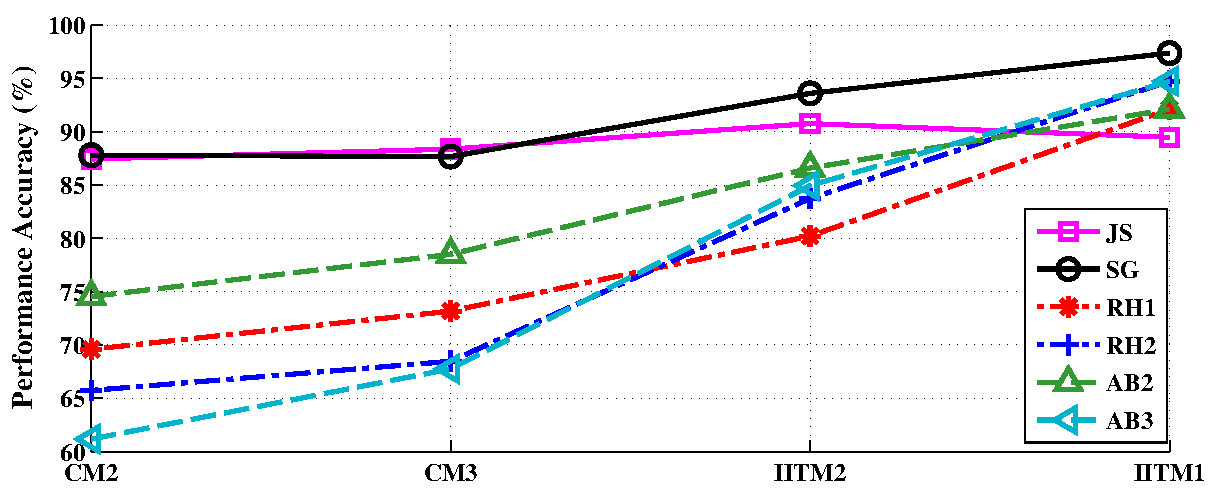
\includegraphics[width=\figSizeNinety]{ch05_preprocessing/figures/Accuracy_Length.pdf}
	\end{center}
	\caption[Tonic identification accuracies of different approaches on four datasets]{Accuracy (\%) of different methods on four datasets arranged by increasing order of mean duration. Only the subscript in the names of the methods and datasets is used for labeling the axis and legends.}
	\label{fig:tonic_id_accuracy_vs_length}
\end{figure}


We now proceed to analyze the tonic identification accuracy as a function of the excerpt duration. As shown in~\tabref{tab:tonic_datasets}, different datasets contain audio excerpts of different lengths. In order to investigate a possible correlation between the accuracy of a method and the length of an audio
excerpt, in~\figref{fig:tonic_id_accuracy_vs_length}, we plot the identification accuracies of different methods for four of the six datasets ordered
by the mean duration of the excerpts: \acrshort{tds_cm2} (3 min), \acrshort{tds_cm3} (full song), \acrshort{tds_iitm2} (full song) and \acrshort{tds_iitm1} (full concert). \acrshort{tds_cm1} and \acrshort{tds_iisc} are excluded because the characteristics of these datasets are very different compared to the rest of the datasets (\acrshort{tds_cm1} contains only instrumental performances and \acrshort{tds_iisc} has poor quality audio). As could be expected, from~\figref{fig:tonic_id_accuracy_vs_length} we notice that practically for all methods there is an improvement in the performance as we increase the duration
of the excerpts. Interestingly, the improvement is very significant for the predominant pitch-based methods (\acrshort{tonicid_ranjani_1}, \acrshort{tonicid_ranjani_2}, \acrshort{tonicid_ashwin_2} and \acrshort{tonicid_ashwin_3}) compared to the multipitch-based methods (\acrshort{tonicid_justin} and \acrshort{tonicid_sankalp}). This shows that the latter approaches, which exploit the pitch information of the drone instrument require less amount of audio data to perform this task. Notably, the accuracy of \acrshort{tonicid_justin} remains nearly the same across all the datasets, which is because the normalized distribution of the tones corresponding to the drone sound remains the same throughout the excerpt. Since this method does not utilize the predominant pitch information, it does not benefit much from the long duration audio excerpts. Note that, while the TP accuracy by \acrshort{tonicid_justin} is the lowest compared to the other methods on \acrshort{tds_iitm1} dataset, the TPC accuracy is amongst the highest. 

\begin{figure}
	\begin{center}
		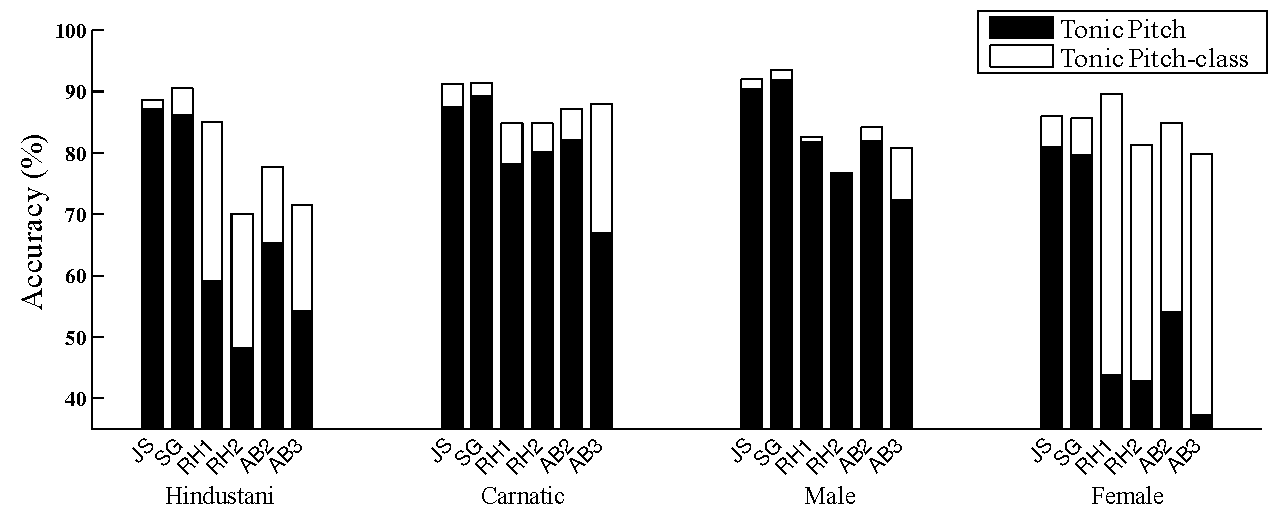
\includegraphics[width=\figSizeHundred]{ch05_preprocessing/figures/Category_Performance.pdf}
	\end{center}
	\caption[Tonic identification accuracies for Hindustani, Carnatic, male and female excerpts]{Accuracy (\%) as a function of different attributes (Hindustani, Carnatic, male, female).Only the subscript in the names of the methods is used for labeling the axis.}
	\label{fig:tonic_id_categorywise_performance}
\end{figure}

In addition to analyzing the performance accuracy for the whole dataset, we also examine the results as a function of different musical attributes of a dataset, namely music tradition (Hindustani or Carnatic) and the gender of the lead singer (male or female). For this analysis, we use the \acrshort{tds_cm2} dataset, as it has the most balanced representation of excerpts from the different categories. In~\figref{fig:tonic_id_categorywise_performance}, we show the accuracies obtained by the different methods as a function of the different attributes. We see that the performance of the multipitch-based approaches (\acrshort{tonicid_justin} and \acrshort{tonicid_sankalp}) is relatively independent of the music tradition (Hindustani or Carnatic). On the other hand, for the predominant pitch-based approaches there is a significant difference in performance for Hindustani and Carnatic music. They obtain considerably better results on Carnatic music. The most notable difference for these approaches is the increased amount of octave errors made for Hindustani music compared to Carnatic music (deduced from the difference seen in tonic pitch-class and the tonic pitch accuracies). A possible reason for this is that in the Hindustani recordings the \gls{tanpura} is generally more salient compared to the Carnatic recordings. This results in the monophonic pitch estimators tracking the \gls{tanpura} in some frames, in particular, when the lead artist is not singing. As a result, the pitch histogram includes high peaks at octave multiples or sub-multiples of the correct tonic pitch. In the case of \acrshort{tonicid_ashwin_2}, \acrshort{tonicid_ashwin_3}, \acrshort{tonicid_ranjani_1} and \acrshort{tonicid_ranjani_2}, most octave errors were found to be sub-multiples of the tonic pitch, possibly caused by the salient lower Sa played by the drone instrument.

Now we turn to examine the performance as a function of the gender of the lead artist (male or female). We see that in general, all the approaches function better
for the performances by the male singers compared to those by the female singers. Similar to the case across music traditions, the difference is more significant for the predominant pitch-based methods, which make a large number of octave errors for the performances by the female singers. As noted earlier (\secref{sec:tonic_selection}), in methods \acrshort{tonicid_ranjani_1}, \acrshort{tonicid_ranjani_2}, \acrshort{tonicid_ashwin_2} and \acrshort{tonicid_ashwin_3} a range of 100-250 Hz is considered for finding the tonic pitch when no additional metadata about the artists is available. In the case of female singers, the tonic usually resides in the higher end of this range. However, the presence of the drone, the tonal sounds produced by percussive instruments and the octave errors produced by the pitch tracker, all contribute to the appearance of a high peak one octave below the tonic of the female singers. This is especially the case for three minute excerpts, wherein a limited amount of vocal pitch information is available. In the case of the approaches based on multipitch analysis and classification (\acrshort{tonicid_justin} and \acrshort{tonicid_sankalp}), a probable reason for obtaining better performance for male singers is the larger number of excerpts from male singers in the database. As a result, it is possible that the rules learned by the classifier are slightly biased towards the performances of male singers.


\subsubsection{Results Obtained Using Metadata Together with the Audio}
\label{sec:pre_processing_tonic_id_results_with_metadata}

One of the ways to reduce the amount of octave errors in tonic identification is to restrict the frequency range of the allowed tonic pitches. The frequency range can be optimized based on the additional information regarding the gender of the singer (when available) to guide the method. In this section, we analyze the effect of including information regarding the gender of the singer and the performance type (vocal or instrumental) on the identification accuracy obtained by the methods.

\setlength{\tabcolsep}{4pt}
\begin{table}
\begin{centering}
	\begin{tabular}{ c | c  c  c  c  c  c }
\tabletop
		{Methods}  & \acrshort{tds_cm1} & \acrshort{tds_cm2} & \acrshort{tds_cm3} &	\acrshort{tds_iisc} & \acrshort{tds_iitm1} & \acrshort{tds_iitm2}\\
\tablemid
		\acrshort{tonicid_justin} & 88.9 & \textbf{93.6} & 92.4 & 80.9 & \textbf{97.4} & 92.3 \\
		
		\acrshort{tonicid_sankalp} & 92.2 & 90.9 & 90.5 & 85.3 & \textbf{97.4} & \textbf{93.6}  \\
		\hdashline
		\acrshort{tonicid_ranjani_1} & 87.7 & 83.5 & 88.9 & \textbf{87.3} &\textbf{ 97.4} & 91.7 \\
		
		\acrshort{tonicid_ranjani_2} & 79.55 & 76.3 & 82 & 85.5 & \textbf{97.4} & 91.5 \\
		
		\acrshort{tonicid_ashwin_1} & - & - &- & - & \textbf{97.4} & - \\
		
		\acrshort{tonicid_ashwin_2} & \textbf{92.3} & 91.5 & \textbf{94.2} & 81.8 & \textbf{97.4} & 91.1 \\
		
		\acrshort{tonicid_ashwin_3} & 87.5 & 86.7 & 90.9 & 81.8 & \textbf{94.7} & 89.9 \\
\tablebot		
	\end{tabular}
\par	\end{centering}
	\caption[Tonic identification accuracies of seven methods on six different datasets using both audio and editorial metadata]{Accuracies (tonic pitch-class (\%)) when additional information regarding the gender of the lead singer (male/female) and performance type (vocal/instrumental) is used. The dashed horizontal line divides the methods based on supervised learning (\acrshort{tonicid_justin} and \acrshort{tonicid_sankalp}) and those based on expert knowledge (\acrshort{tonicid_ranjani_1}, \acrshort{tonicid_ranjani_2}, \acrshort{tonicid_ashwin_1}, \acrshort{tonicid_ashwin_2} and \acrshort{tonicid_ashwin_3}).}
	\label{tab:tonic_identification_accuracy_with_gender_info}
\end{table}

In~\tabref{tab:tonic_identification_accuracy_with_gender_info}, we present the identification accuracies obtained when associated metadata is available to the methods in addition to the audio data. Note for this evaluation we only report the tonic pitch
accuracy for vocal excerpts (and not pitch-class accuracy) since when this metadata is available the pitch range of the tonic is known and limited to a
single octave, meaning the TP and TPC accuracies will be the same.

Comparing the identification accuracies summarized in~\tabref{tab:tonic_identification_accuracy_with_gender_info} with the with ones in~\tabref{tab:tonic_identification_accuracy_without_gender_info}, we see that the accuracies for all methods are higher when gender and performance metadata is available. With the additional information the performance of the predominant pitch-based approaches (\acrshort{tonicid_ashwin_2}, \acrshort{tonicid_ashwin_3} and \acrshort{tonicid_ranjani_1}) becomes closer to that of the multipitch-based approaches (\acrshort{tonicid_justin} and \acrshort{tonicid_sankalp}). Whilst the performance of all methods is improved, the increase in accuracy is more considerable for the predominant pitch-based approaches which use template matching (in particular \acrshort{tonicid_ashwin_2} and \acrshort{tonicid_ashwin_3}) compared to classification-based approaches (\acrshort{tonicid_justin} and \acrshort{tonicid_sankalp}). This possibly indicate that the rules learned automatically using machine learning are more complete compared to the relatively simple Sa-Pa templates, meaning that the classification-based approaches can correctly identify the octave of the tonic even without using gender metadata. That is, since both male and female excerpts are used during training, the influence of the gender of the singer on the pitch features is implicitly learned by the classifier, thus producing rules that can handle both male and female performances, even without explicit metadata about the gender of the singer. On the other hand, manually defined template-based approaches require this extra information to fine-tune the frequency range
considered for the tonic, after which they obtain comparable performance to that of the classification-based methods.

A potential advantage of the template-based approaches is that they do not require training. This, in theory, could make them more generalizable compared
to the classification-based methods. To assess this, we ran an experiment in which the classification-based approaches were trained on one dataset and tested on a different dataset (\acrshort{tds_cm2} and \acrshort{tds_iitm2}). We found that the results only went down by approximately 2\% compared to the results obtained using 10-fold cross validation on a single dataset. Furthermore, the datasets used for this experiment contained relatively different music material (percentage of Carnatic music excerpts and length of the audio files). This suggests that for tonic identification the rules learned by the classification-based approaches are generalizable and can be used to obtain high identification accuracies on diverse and sizable music collections of \gls{iam}.


\subsubsection{Error Analysis}
\label{sec:pre_processing_tonic_identification_error_analysis}

We now turn to analyze the different types of errors made by the methods, both with and without using additional metadata for each dataset. Overall, three common types of errors are identified: Pa errors, where the fifth (Pa) is selected instead of the tonic, Ma errors, where the fourth (Ma) is selected instead of the tonic, and the previously mentioned octave errors, where the correct pitch is identified but in the wrong octave (usually one octave above or below the
tonic). Since the octave errors are already discussed at length in the previous paragraphs, here we focus on all other types of errors, which we divide into three categories: Pa (for Pa errors), Ma (for Ma errors) and ``Other'', which includes all errors that are neither Pa, Ma nor octave errors (e.g.~selecting the seventh (\gls{ni}) instead of the tonic Sa).


\begin{figure}
	\begin{center}
		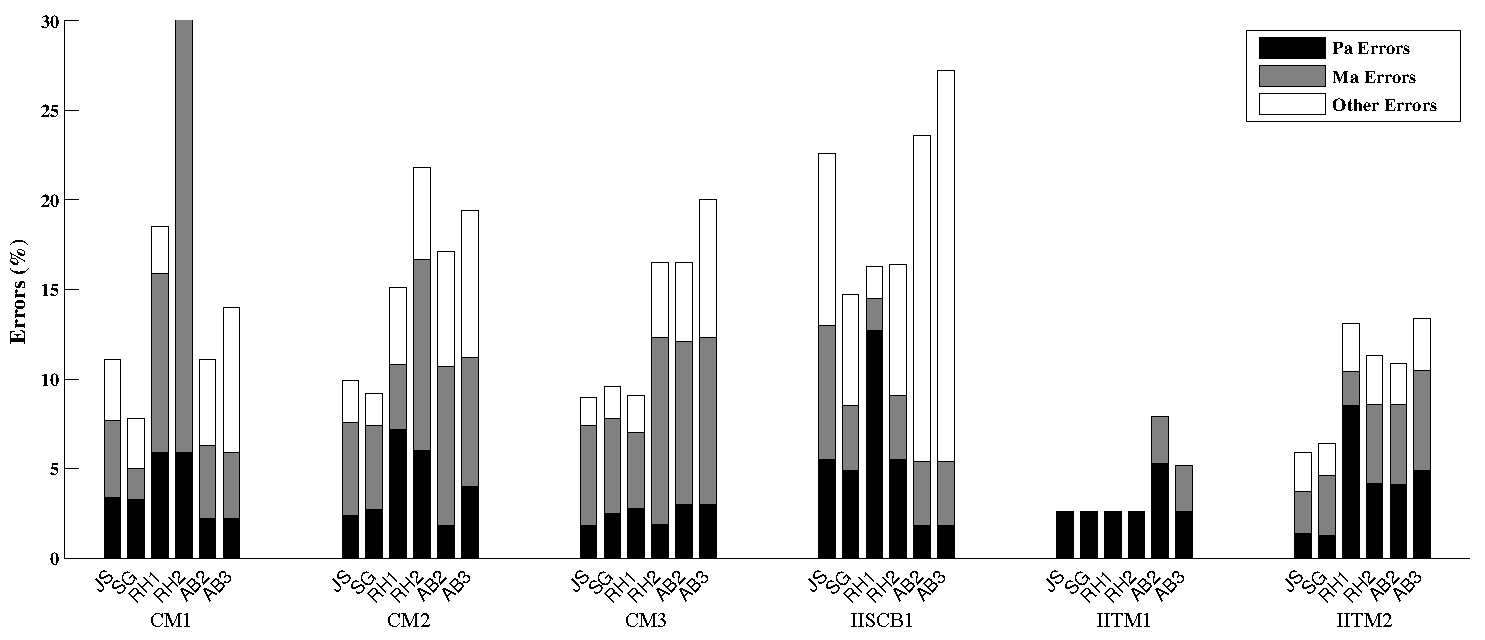
\includegraphics[width=\figSizeHundred]{ch05_preprocessing/figures/ErrorAnalysis_Without_MF.pdf}
	\end{center}
	\caption[Percentage of Pa, Ma and `Other' type errors in tonic identification]{Percentage of excerpts containing each of the three different categories of errors (excluding octave errors): Pa, Ma and Other, when no additional metadata is used. Only the subscript in the names of the methods and datasets is used for labeling the axis.}
	\label{fig:tonic_identification_errors_without_MF}
\end{figure}

In~\figref{fig:tonic_identification_errors_without_MF}, for each dataset, we show the percentage of excerpts containing each of the three categories of errors for every method (when no additional metadata is used). We see that for most datasets Pa and Ma errors constitute a large proportion of the total amount of errors made by each method. These confusions make sense from a musical perspective, since in every performance of \gls{iam} one of these two \glspl{svara} (Pa or Ma) is always present in a melody in addition to Sa (the tonic pitch-class). Furthermore, the pitch distance between Sa and Pa (fifth) is
the same as the distance between Ma and higher Sa, and the pitch distance between Sa and Ma (one fourth) is same as the distance between between Pa and higher Sa. Since most approaches are based on templates or rules that consider the pitch distance between the peaks of the feature histogram, these equivalences can
cause four types of confusions: considering a Sa-Pa pair to be Ma-Sa leading to a Pa error, considering Ma-Sa to be Sa-Pa leading to a Ma error, considering
Sa-Ma to be Pa-Sa leading to a Ma error and considering Pa-Sa to be Sa-Ma leading to a Pa error.

For the approaches based on multipitch analysis (\acrshort{tonicid_justin} and \acrshort{tonicid_sankalp}), we observe that the only case where we get more `Other' errors compared to Pa and Ma errors is for the \acrshort{tds_iisc} dataset. Since the drone sound is very weak in the excerpts of this dataset, there are cases in which the prominent peaks of the multipitch histogram correspond to \glspl{svara} other than Sa, Ma and Pa (which depends on the choice of the \gls{raga}). Since these approaches assume that the multipitch histogram represents the \glspl{svara} of the drone instrument, the peaks of the histogram are mistakenly identified as Sa and Pa or Sa and Ma, leading to an error in identification. For these specific type of excerpts the \acrshort{tonicid_ranjani_1} method produces slightly better results, as the \gls{shadja} is not inflected (i.e. there is little pitch variation within the \gls{svara}) regardless of the \gls{raga}.

\begin{figure}
	\begin{center}
		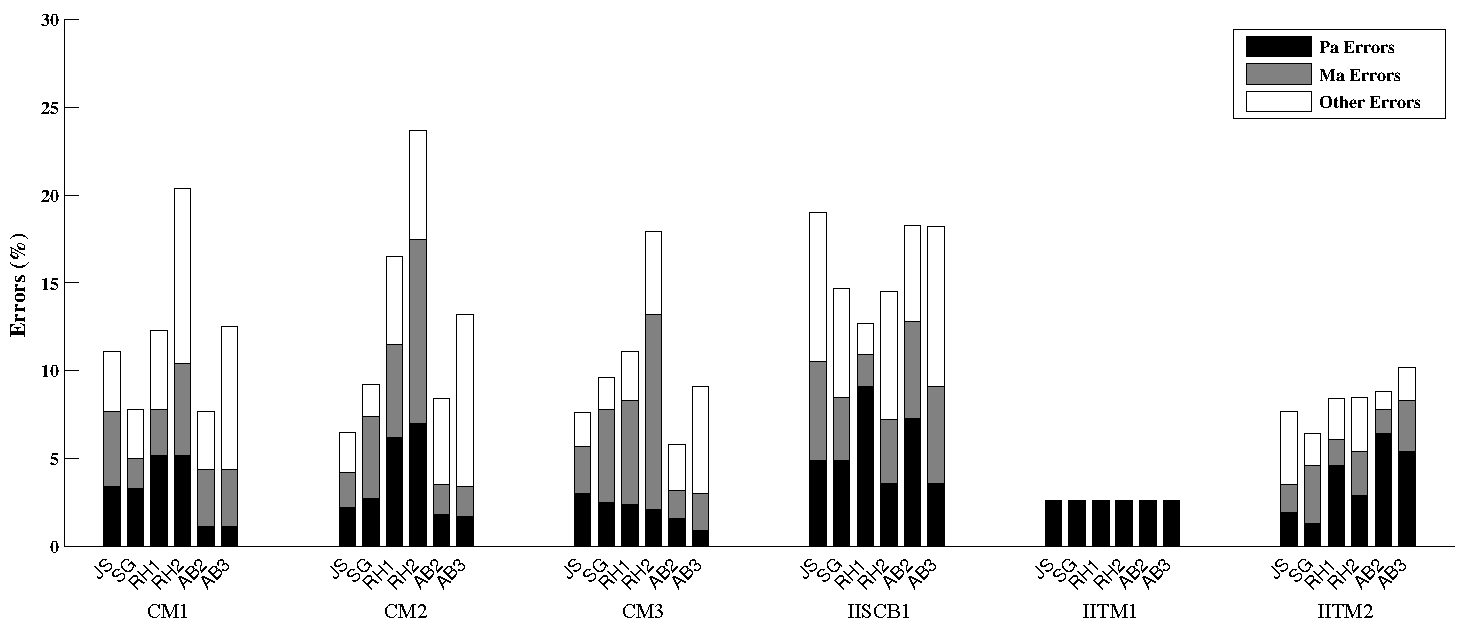
\includegraphics[width=\figSizeHundred]{ch05_preprocessing/figures/ErrorAnalysis_With_MF.pdf}
	\end{center}
	\caption[Percentage of Pa, Ma and `Other' type errors in tonic identification, using editorial metadata]{Percentage of different type of errors (Pa, Ma and Others) by different methods on all the datasets using information regarding the gender of the singer and performance type. Only the subscript in the names of the methods and datasets is used for labeling the axis.}
	\label{fig:tonic_identification_errors_with_MF}
\end{figure}

In many cases we observe that the percentage of Ma errors is greater than the percentage of Pa errors. For the classification-based approaches, this can be
attributed to the fact that in most excerpts the drone instrument is tuned to Pa tuning (lower Sa, middle Sa, middle Sa, lower Pa). This creates a
bias in the training set and the rules learned by the classifier work better for Pa tuning. Ma errors are also common in \acrshort{tonicid_ranjani_2}, as the estimator looks for a Sa-Pa-higher Sa pitch relation, which would also fit a Ma-tuned performance. \acrshort{tonicid_ranjani_1} on the other hand does not search for a Sa-Pa-Sa template, resulting in a low proportion of Ma errors compared to the other methods. Finally we note that most methods do not make any Ma errors on the \acrshort{tds_iitm1} dataset. This is because the items in this dataset are full concerts, each concert consisting of several pieces. Whilst Ma may be included in the melody of some of the pieces, Pa and Sa are always present. As a result, the pitch histogram for the complete concert does not contain a prominent Ma peak, meaning that it is highly unlikely for it to be selected as the tonic.



We examine how the errors are affected once we allow methods to use gender and performance metadata~(\figref{fig:tonic_identification_errors_with_MF}). If we compare the results to those in~\figref{fig:tonic_identification_errors_without_MF}, we see
that Ma and Pa errors are reduced more than ``Other'' errors. By restricting the tonic frequency range to a single octave we prevent the
appearance of a high Sa peak, thus avoiding the possible confusion between fourths and fifths explained earlier and reducing the amount of Pa and Ma errors.

For \acrshort{tonicid_ranjani_1} and \acrshort{tonicid_ranjani_2} the percentage of Ma errors actually increases slightly after including male/female information. A large proportion of these errors were observed in excerpts with female singers. For these excerpts, the range for \gls{shadja} candidates is limited to 130-250 Hz. For this range, candidates fitting a lower Ma-middle Sa-middle Ma template would also satisfy the minimization criterion used in \acrshort{tonicid_ranjani_2}. In the case of \acrshort{tonicid_ranjani_1}, the reduced frequency range results in relatively weak peaks also being considered, and their small pitch variance can result in the wrong candidate being selected during the minimization process.

\begin{figure}
	\begin{center}
		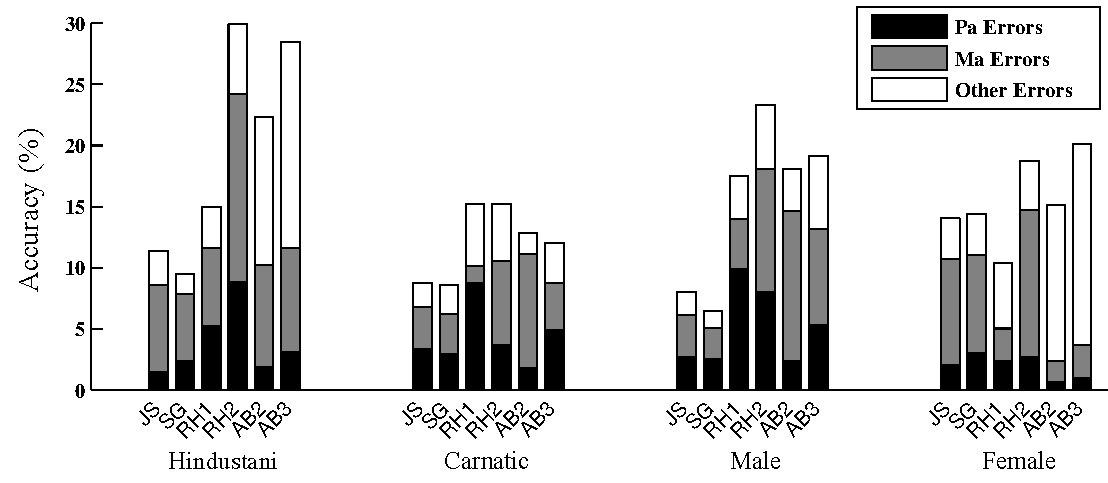
\includegraphics[width=\figSizeHundred]{ch05_preprocessing/figures/Category_Errors.pdf}
	\end{center}
	\caption[Percentage of Pa, Ma and `Other' type errors in tonic identification for different categories]{Percentage of excerpts with the different categories of errors (Pa, Ma and Others) for every method as a function of different excerpt attributes (Hindustani, Carnatic, male, female). Only the subscript in the names of the methods is used for labeling the axis.}
	\label{fig:tonic_identification_categorywise_errors}
\end{figure}

Finally, we analyze the errors as a function of the different attributes of the excerpts (Hindustani versus Carnatic, male versus female). As in~\secref{sec:pre_processing_tonic_id_results_only_audio_data}, we use the \acrshort{tds_cm2} dataset for this analysis because it is the most balanced dataset in terms of these attributes. Note that the methods are not provided with any metadata in addition to the audio signal. The percentage of excerpts containing each of the three categories of errors (Pa, Ma and Other) for every approach as a function of the different excerpt attributes is shown in ~\figref{fig:tonic_identification_categorywise_errors}. We see that for the classification-based methods, the proportion of Ma errors is much higher in performances by female singers compared to performances by male singers. The pitch range of the tonic for female singers is such that the lower Ma resides in the frequency range where the tonic of most male singers lies. Thus, the lower Ma-middle Sa (fifth) relationship for female singers is often confused with middle Sa-Pa relationship for male singers, resulting in a high number of Ma errors. For further details and insights regarding the types of error made by the
different methods and their underlying causes we refer the reader to the publications where these methods are discussed in depth \citep{salamon2012multipitch, SGulati_MThesis2012,bellur2012knowledge,ranjani2011carnatic}.


\subsection{Summary of the Comparative Evaluation }
\label{sec:pre_processing_tonic_identification_summary}

We evaluated seven tonic identification methods on six different and diverse datasets of \gls{iam}. The evaluation was performed in two scenarios: first, when only audio data is used as input to the methods, and second, when the additional information about the gender of the singer (male or female) and the performance type (vocal or instrumental) is given in addition to audio data. The results obtained are analyzed per dataset, and for different characteristics of the music material. Along with the accuracies of the methods, we presented an in-depth error analysis, describing the different kinds of errors for different scenarios and provided plausible explanations for them.

Overall, we see that methods \acrshort{tonicid_justin} and \acrshort{tonicid_sankalp} that use multipitch-based audio feature and classification methodology for selecting tonic pitch perform better than the rest. Their performance is better on all but one datasets considered in the evaluation (the exceptional dataset is small in size and contains poor quality audio recordings). In addition, the performance of these two methods appears to be the most consistent across music traditions, gender of the singer (male or female) and type of music performance (vocal or instrumental). 

Finally, we select \acrshort{tonicid_justin} method to identify tonic pitch from audio recordings in all the studies conducted as a part of this thesis. \acrshort{tonicid_justin} produces comparable results to \acrshort{tonicid_sankalp} and is relatively simpler to implement owing to a single stage processing. Furthermore, \acrshort{tonicid_justin} does not require any estimate of the predominant pitch, which makes it independent of the performance of the pitch estimation algorithms. The are two implementations of this method, which we make publicly available online~(\appref{app:resources}).


\subsection{Correcting Common Errors in Tonic Identification}
\label{sec:pre_processing_tonic_identification_correcting_errors}

As mentioned above, identification of the tonic pitch is a crucial first step required for nearly all meaningful melodic analyses of \gls{iam}. Any error in this step propagates through the processing chain and adversely affect the output of the melodic analyses. Though the accuracy of the most successful tonic identification method is nearly 90\% (\tabref{tab:tonic_identification_accuracy_without_gender_info}), even a 10\% error in tonic pitches can deteriorate the performance of melodic analyses described in the subsequent chapters. Moreover, it leads to an uncertainty, whether an error in the final output is caused due to a wrong tonic pitch or it is because of an error made in the later stages of the methods. 

We here present an heuristic-based approach to correct frequently occurring errors in tonic identification. From \tabref{fig:tonic_identification_errors_without_MF}, we see that the majority of the errors are Ma and Pa errors. Also, we know from the music knowledge that the tonic pitch chosen by the lead performers in \gls{iam} does not change drastically over the years and it typically remains within two semitones (200\,Cents). Since the accuracy of the tonic identification is nearly 90\%, for the recordings of an artist in our music corpus there might only be a handful of recordings for which the tonic values are incorrectly identified. Moreover, these wrong estimates are either Ma or Pa. These errors typically correspond to a pitch value that cannot possibly be the true tonic of the singer. Thus, these erroneous cases can be automatically detected by employing a majority voting. Once detected, the wrongly estimated tonic values can be transposed (either by fifth, or fourth) to match the most frequent tonic value of that artist in the corpus. After we perform this step, we achieve close to perfect tonic estimates for the music collection. %As can be imagined, this approach would work for artists that have more than a certain number of recordings in the collection. Since the recordings are ripped from the complete CDs, most of the artists considered in the datasets do have reasonable number of recordings in our corpus.


\section{Melody Processing}
\label{sec:data_preprocessing_melody_processing}

In this section, we present all the procedures applied in relation to the extraction and processing of a melody representation from raw audio signals. These processing steps can be grouped into three main categories: predominant pitch estimation (sometimes also referred to as predominant melody extraction), pitch post-processing, and melody representation. All these three steps are described at length in the subsequent sections. 

\begin{figure}
	\begin{center}
		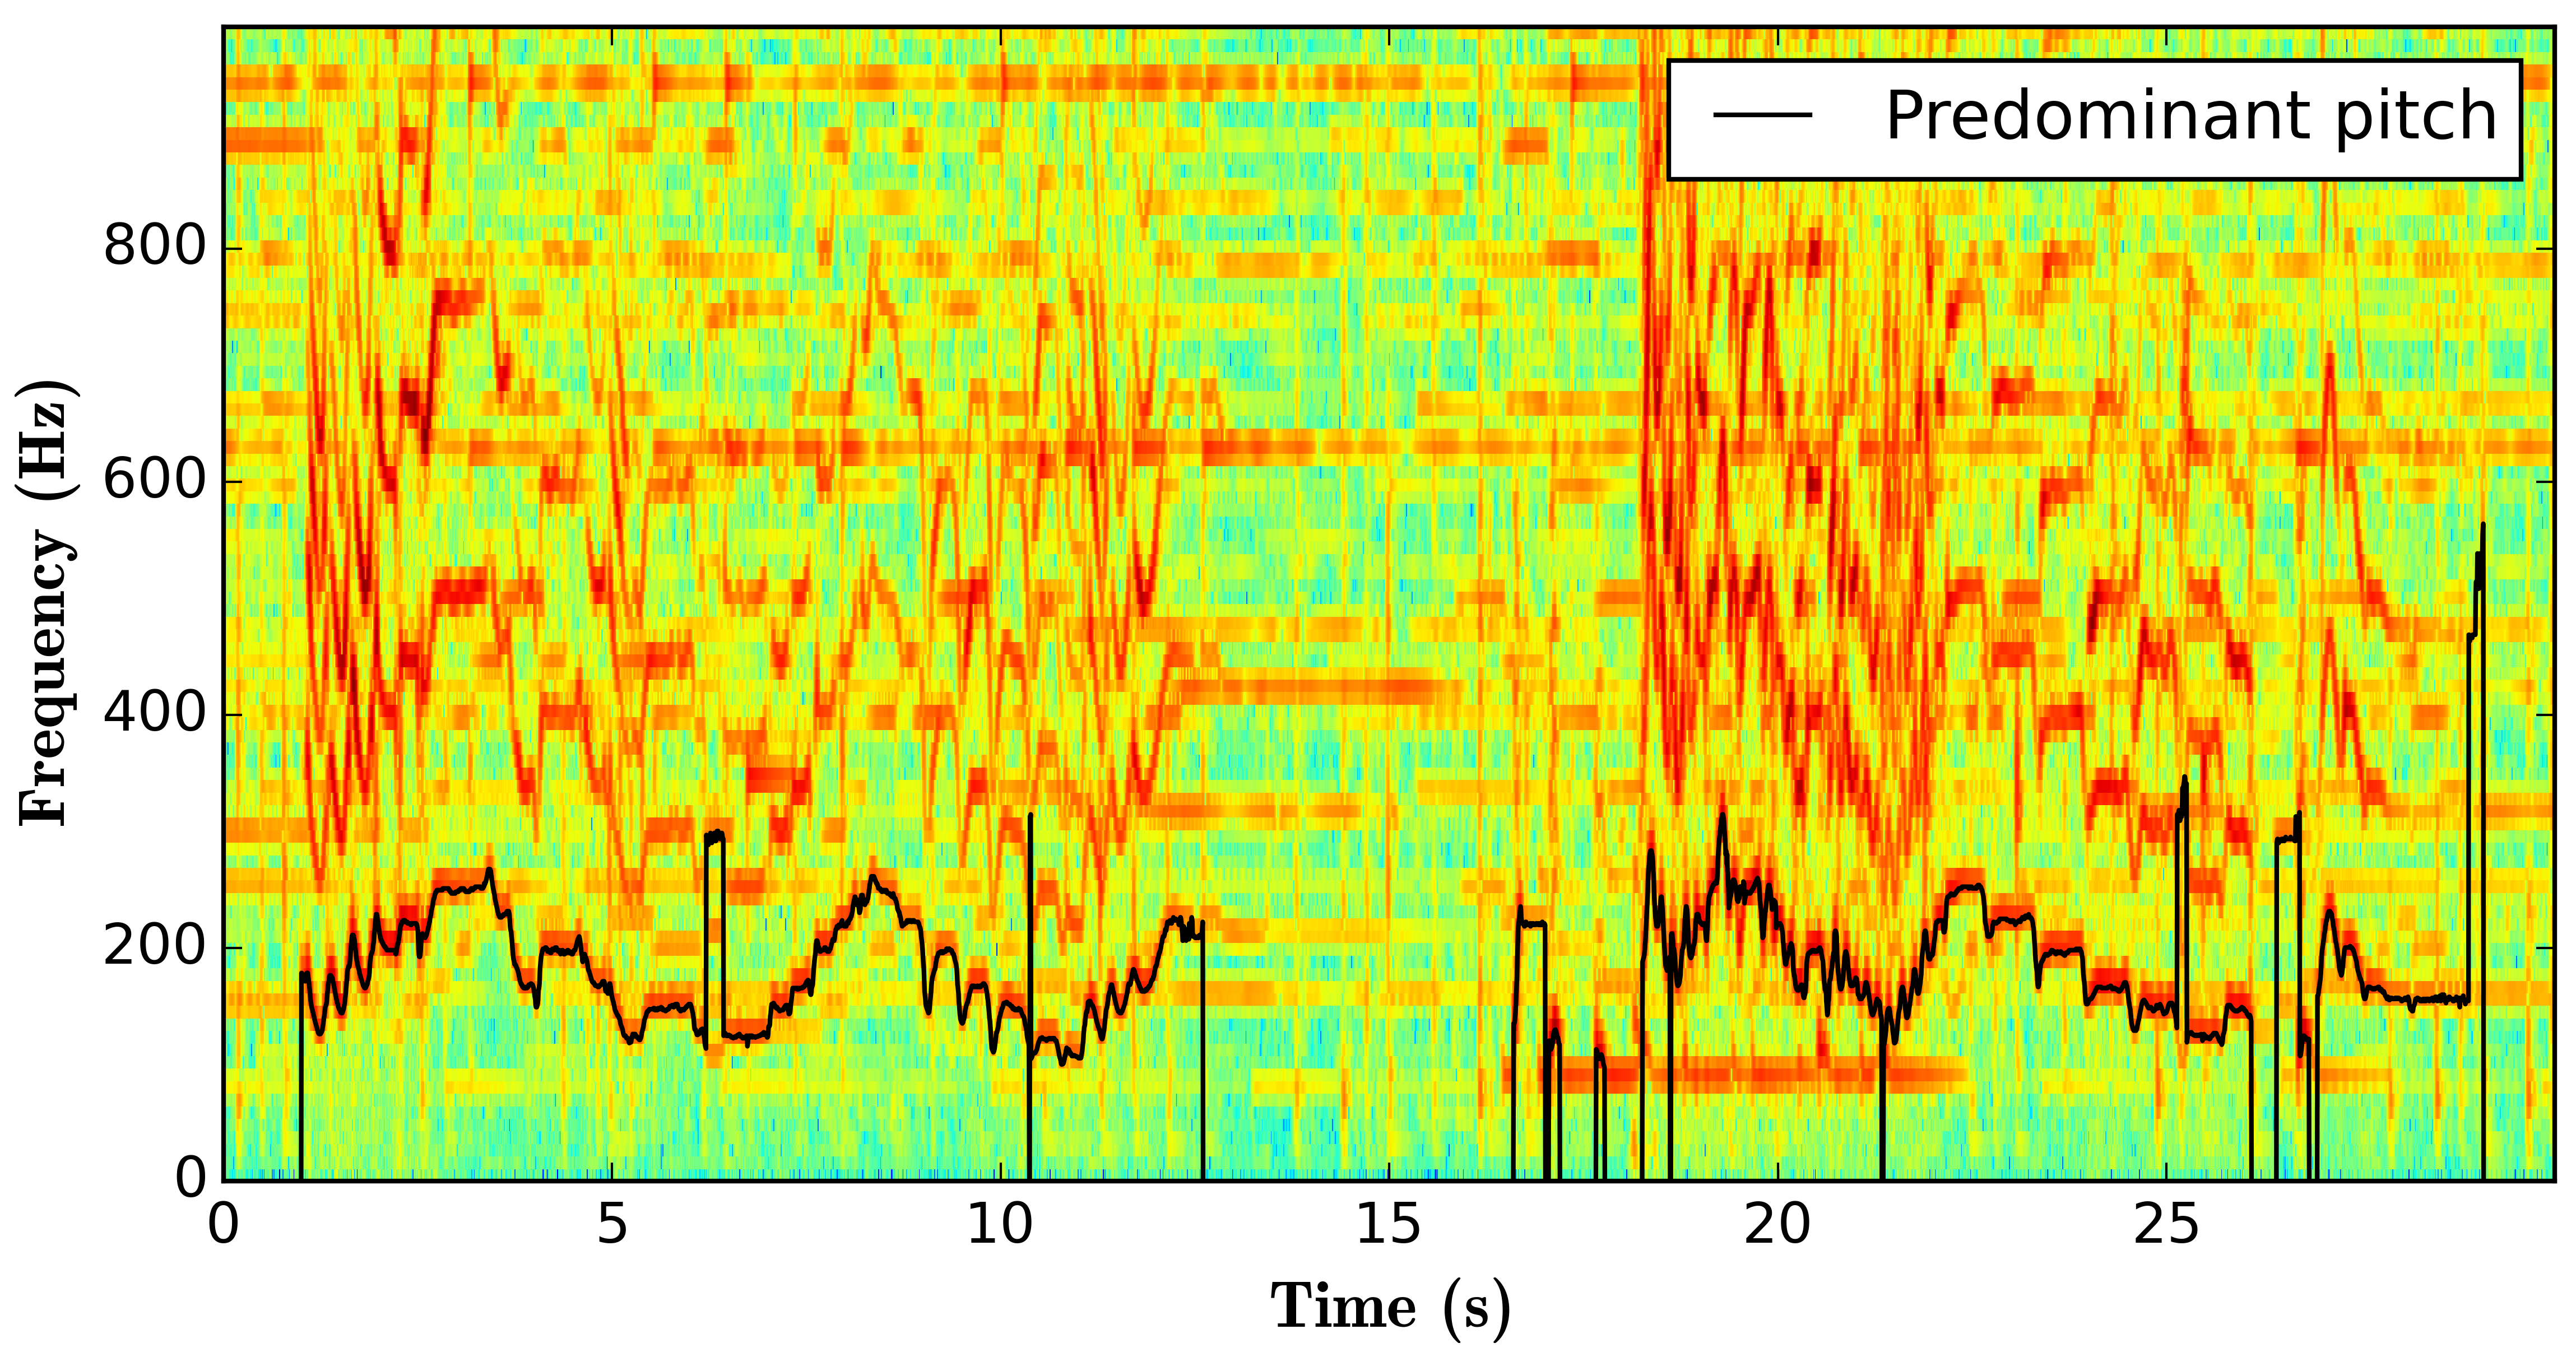
\includegraphics[width=\figSizeHundred]{ch05_preprocessing/figures/predominantMelodyExample.png}
	\end{center}
	\caption[Example of the predominant pitch representation of melody]{Example of a continuous pitch contour corresponding to the predominant melodic source extracted from a polyphonic audio excerpt}
	\label{fig:predominant_melodic_fragment}
\end{figure}


\subsection{Predominant Pitch Estimation}
\label{sec:data_preprocessing_predominant_melody_estimation}

In \secref{sec:background_terminology}, we presented our working definition of melody. In a nutshell, we consider the continuous pitch contour corresponding to the predominant melodic source (typically, the lead artist) in the audio recording as the low-level representation of melody. An example is shown in~\figref{fig:predominant_melodic_fragment}, wherein the contour represents the pitch of the lead singer at each instance in time. Usage of such a melody representation is a common practice in \gls{mir}, and is done for a variety of melody processing tasks across different music traditions~\citep{Dutta2014,Ishwar2013,Rao2014,koduri2014intonation,senturk2013score,pikrakis2012tracking,pikrakis2003recognition,moelants2009exploring}. 

Pitch estimation, also commonly known as pitch tracking from audio signals has been an active research topic since several decades~\citep{salamon:phd:13}. The challenges in the estimation of a reliable pitch contour differ across the type of audio music signals (monophonic or polyphonic). As a result of which the performance of these algorithms vary significantly across different music genres, which also seems to be correlated with the extent of the polyphony in the music. A sparse polyphonic characteristic in audio recordings of \gls{iam} due to its heterophonic nature lessens the complexity of the task to an extent, when compared to several other western popular music genres. This trend is clearly visible from the past MIREX (an international MIR evaluation campaign) results\footnote{\url{http://www.music-ir.org/mirex/wiki/MIREX_HOME}}. For example, compare the accuracy obtained by different algorithms on INDIAN08\footnote{\url{http://nema.lis.illinois.edu/nema_out/mirex2011/results/ame/indian08/summary.html}},  MIREX05\footnote{\url{http://nema.lis.illinois.edu/nema_out/mirex2011/results/ame/mirex05/summary.html}} and  MIREX09~0dB\footnote{\url{http://nema.lis.illinois.edu/nema_out/mirex2011/results/ame/mirex09_0dB/summary.html}} datasets from MIREX-2011. 

In order to estimate the predominant pitch (denoted hereafter by $\pitchHz$) in the audio recordings of \gls{iam} we use \gls{melodia} algorithm, a state-of-the-art melody extraction method proposed by~\cite{Salamon2012}. This method performed favorably in MIREX~2011 on a variety of music genres, including \gls{iam}\footnote{\url{http://nema.lis.illinois.edu/nema_out/mirex2011/results/ame/indian08/summary.html}}. This method is used in several other studies that analyze melodies extracted from audio signals~\citep{Dutta2014,Ishwar2013,Rao2014,koduri2014intonation,senturk2013score,pikrakis2012tracking}.

Another motivation to use this algorithm is that it works on continuous pitch contours and employs auditory streaming constraints to ensure a continuity in the output pitch. As a result of this processing, it does not produce octave errors at the frame-level. Noticeably, this predominant pitch estimation algorithm also performs voicing detection. This means that the algorithm in addition to estimating the predominant pitch also detects the time segments where the voice is absent. %Such time segments where the predominant melodic source is inactive are assigned a dummy pitch value (usually 0).

Currently, there are two implementations of \gls{melodia} algorithm that are publicly available. We use its implementation as available in \Gls{essentia}~\citep{essentia}. \Gls{essentia}\footnote{https://github.com/MTG/essentia} is an open-source C++ library for audio analysis and content-based MIR. We use the default values of the parameters, except for the frame and hop sizes, which are set to 46 and 2.9\,ms, respectively. The other implementation of \Gls{melodia} is available as a Vamp plug-in\footnote{http://mtg.upf.edu/technologies/melodia}. 

Prior to the predominant pitch estimation we apply an equal-loudness filter\footnote{\url{http://wiki.hydrogenaud.io/index.php?title=ReplayGain_1.0_specification}} to make the processing perceptually relevant~\citep{essentia}. For this operation as well we use Essentia with the default values of the parameters. 

In every computational task addressed in this thesis we use the \Gls{melodia} algorithm to estimate the predominant pitch for all the datasets. There is only one exception, \acrshort{msds_iitb_hmd} dataset, which was introduced in~\cite{Ross2012b} for computing melodic similarity. \acrshort{msds_iitb_hmd} dataset along with audio recordings and melodic phrase annotations also includes semi-automatically extracted predominant pitch contours~(\secref{sec:corpus_melodic_similarity_dataset}). Using the pitch contours provided along with the dataset allows us to compare the output of our method with other studies. In addition, since these pitch contours are nearly free from any octave errors, we avoid propagating errors to subsequent stages, and thus, evaluate the task of melodic similarity more reliably. 

In our work in this thesis we consider only the pitch dimension of melody in its representation. However, loudness and timbral dimensions of melody that largely capture the phonetics and expressive aspects are also informative and can be helpful in several tasks including computation of melodic similarity. To give an idea about the type of information captured in the loudness and timbral dimensions and their usefulness, we take an example. We synthesize the harmonic series corresponding to a voice extracted from an excerpt of Carnatic music. During the synthesis we force the pitch of the voice to a monotone while keeping the other aspects (loudness and timbre) intact. The original excerpt\footnote{\url{http://www.freesound.org/people/sankalp/sounds/352810/}}, synthesized predominant pitch\footnote{\url{http://www.freesound.org/people/sankalp/sounds/352809/}} and the synthesized monotone voice\footnote{\url{http://www.freesound.org/people/sankalp/sounds/352808/}} is made available for listening. After listening to this example, we get an idea about the nature of the melodic characteristics that are not utilized if we only consider the pitch dimension of melody in the analysis. Exploiting loudness and timbral dimensions for melodic analysis shall be taken up in the future endeavors.


\subsection{Pitch Post-processing}
\label{sec:data_preprocessing_pitch_postprocessing}

Predominant pitch estimation in polyphonic audio recordings has not been solved yet, and the output pitch contour is still far from being perfect (MIREX-2011 results\footnote{\url{http://nema.lis.illinois.edu/nema_out/mirex2011/results/ame/indian08/summary.html}}, MIREX-2016 results\footnote{\url{http://nema.lis.illinois.edu/nema_out/mirex2016/results/ame/ind08/summary.html}}). While these algorithms get better over years, a number of errors in the predominant pitch estimation can be alleviated by post-processing the pitch contour. In post-processing, our main objective is to correct the spurious pitch octave jumps and smoothen the extracted pitch contour. In addition, for certain tasks described in the subsequent chapters, we also interpolate the unvoiced regions in the melody that correspond to the short-duration breath pauses taken by the artists. We now describe these post-processing steps in detail.

\subsubsection{Correcting Spurious Pitch Jumps}
\label{sec:data_processing_correcting_pitch_jumps}

\begin{figure}
	\begin{center}
		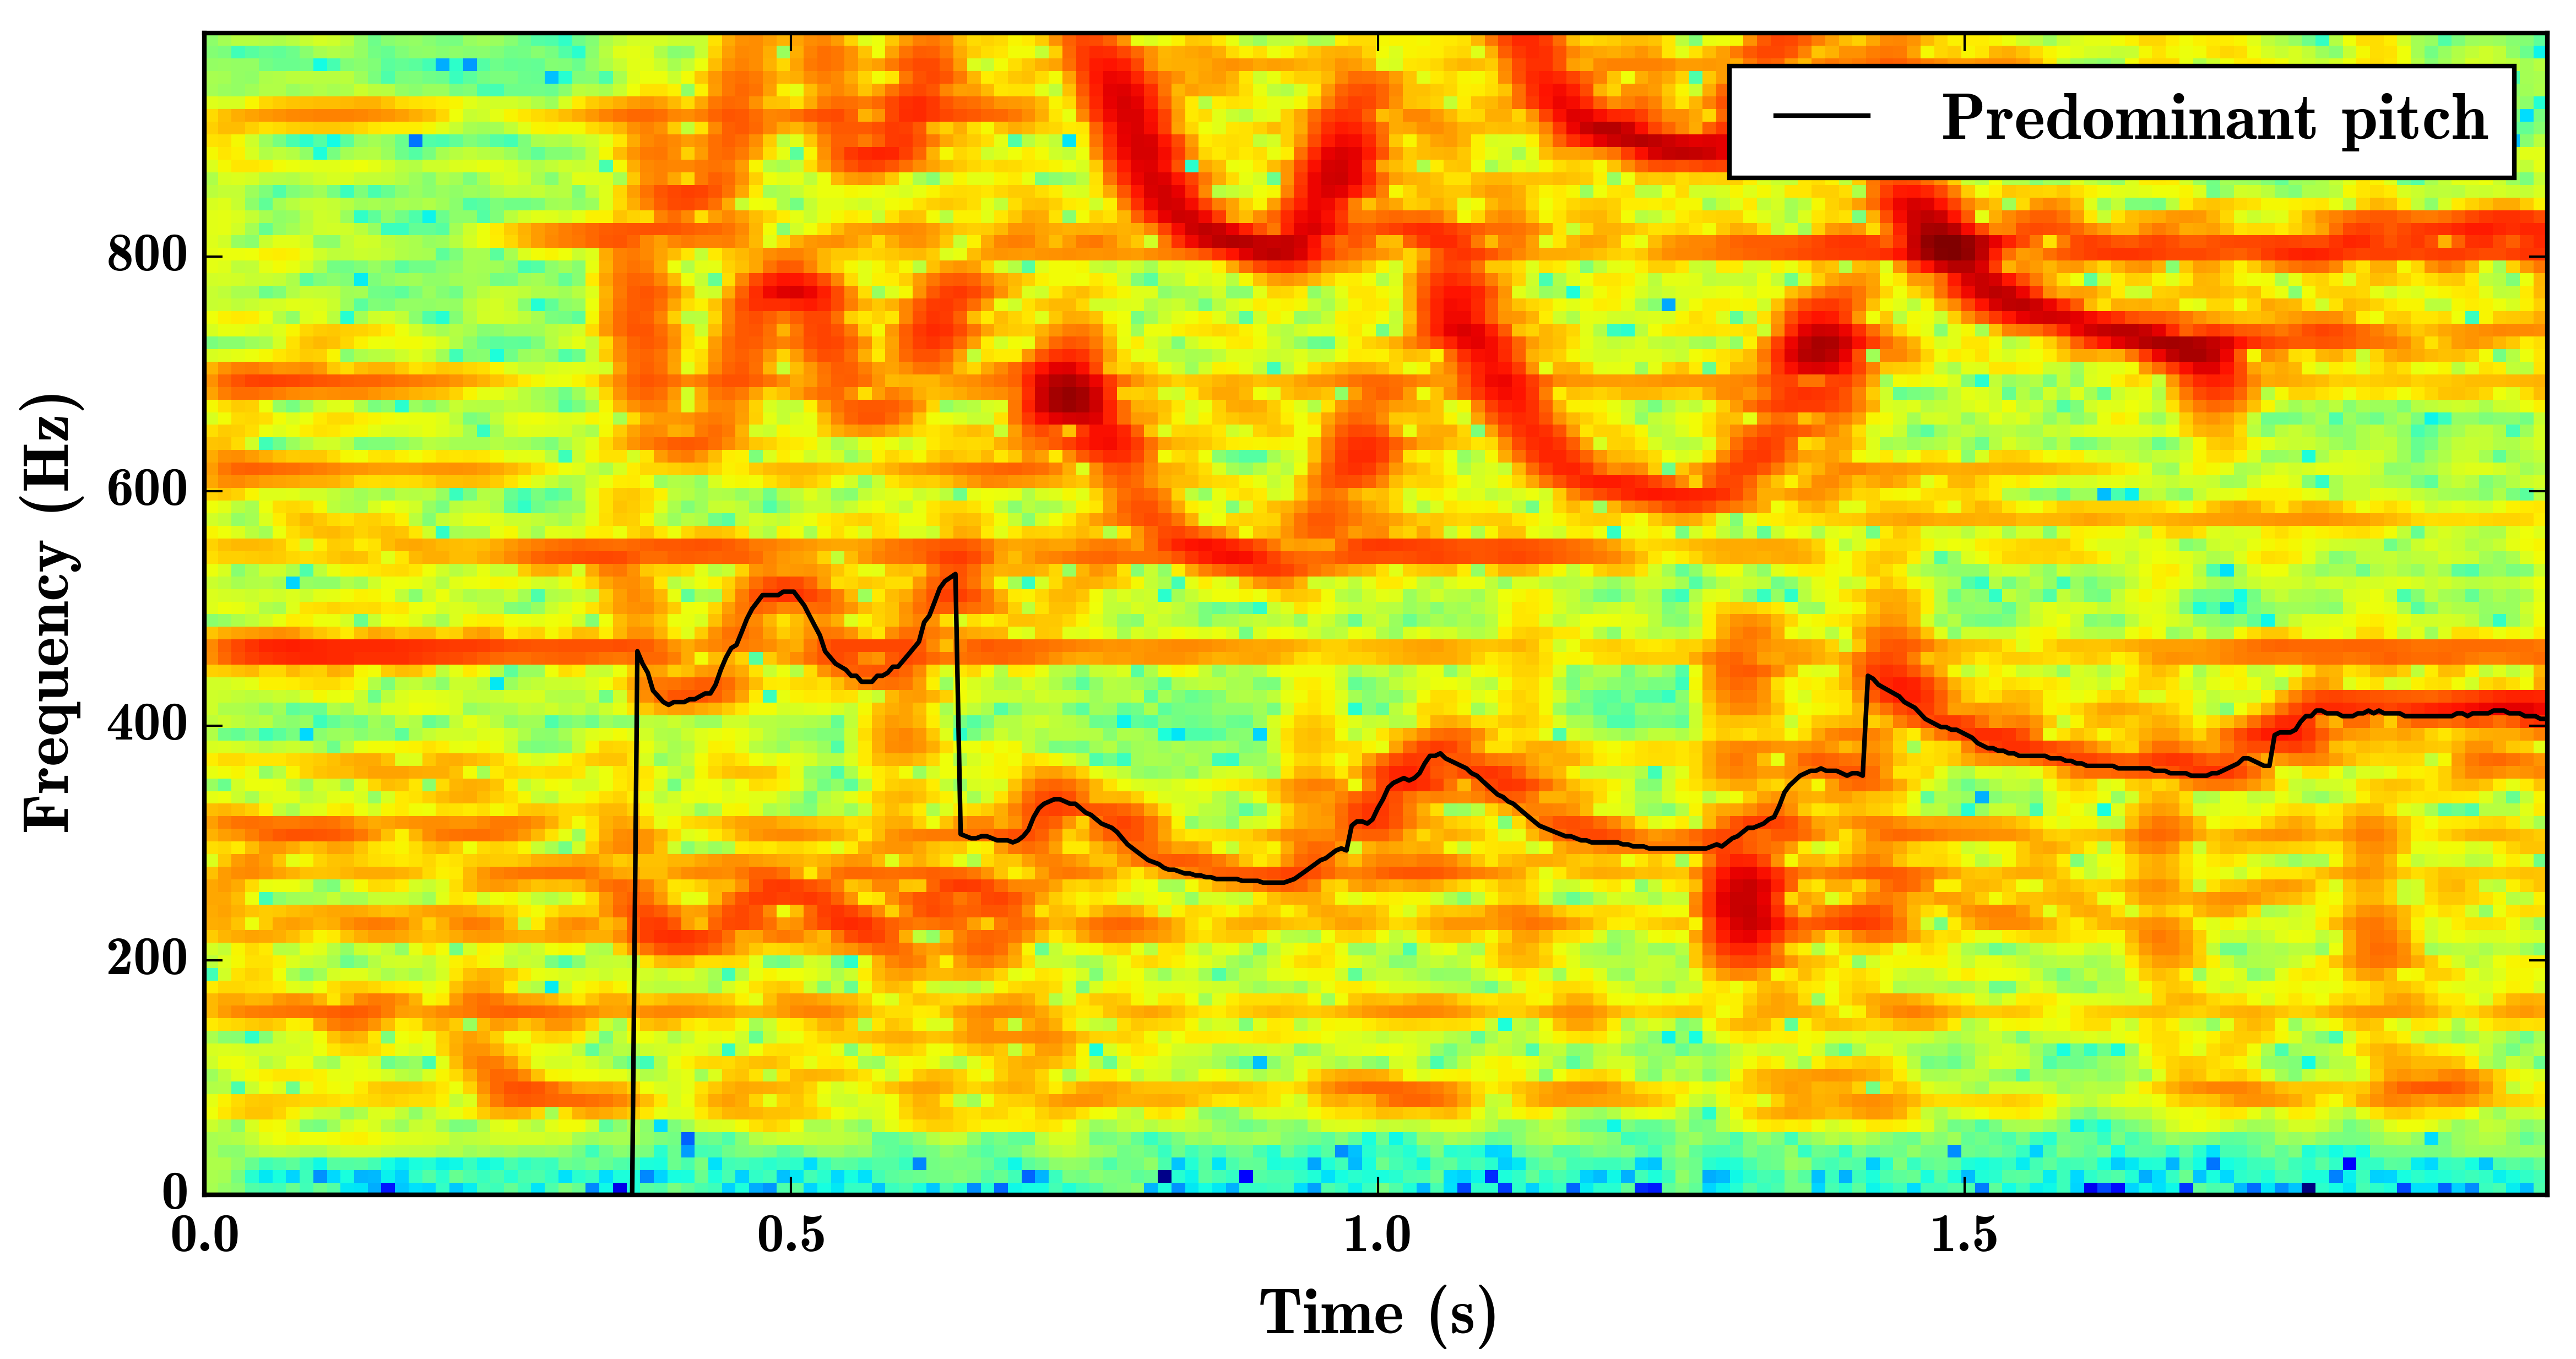
\includegraphics[width=\figSizeHundred]{ch05_preprocessing/figures/octaveErrorIllustration.png}
	\end{center}
	\caption{Example of an octave error in predominant pitch contour}
	\label{fig:octave_error_pitch}
\end{figure}

One of the most frequently occurring errors in pitch estimation is it's detecting in a wrong octave, commonly referred to as an octave error. Identifying and correcting such errors during a post-processing step for the case of a monophonic signal (containing a single harmonic series) is fairly simple. One can compare the energy of the partials with the total energy of the audio frame to infer if the estimated pitch value corresponds to the actual fundamental frequency. However, in the case of a polyphonic music signal it becomes a challenging task. 

We alleviate this problem to an extent by restricting ourselves to a specific type of pitch octave error occurring over a short duration of time. Instead of identifying an octave error for an individual audio frame, we exploit the temporal melodic continuity to detect such errors. We explain the intuition behind our method with the help of an example shown in~\figref{fig:octave_error_pitch}. If we analyze an isolated audio frame at 0.5\,s, identifying a pitch octave error computationally becomes a challenging task. However, by analyzing the pitch continuity we can easily detect an anomalous pitch jump of roughly 1200\,cents at time 0.65\,s. This is due to the fact that such drastic pitch jumps across frames do not occur naturally in singing voice. By analyzing the amount of frequency difference across the pitch transition we can infer to an extent the type of pitch error and can subsequently correct it. Since the detected pitch jump is around 1200\,cents, it is highly likely to be an octave error. In this example voice starts at around 0.4\,s, which we consider as a positive pitch jump. Knowing that there is a anomalous pitch jump in the other direction (negative pitch jump) at time 0.65\,s makes it highly probable that the pitch segment between time 0.4\,s and 0.65\,s suffers from an octave error.  

We describe this heuristic-based approach in~\algoref{alg:algorithmPitchCorrection}. In this algorithm $\mathrm{winSize}$ is set to 1\,s and $\mathrm{silenceCentValue}$ is set to $1200*\log2(\epsilon)$, where $\epsilon$ is of the order of $10^{-17}$.


\renewcommand{\algorithmiccomment}[1]{\bgroup\hfill\tiny//~#1\egroup}

\begin{algorithm}
	\caption{Correcting spurious pitch octave jumps}
	\label{alg:algorithmPitchCorrection}
	\begin{algorithmic}  
		\State {\bf Input:} pitch sequence ($\pitchHz$) of length N samples in Cents scale
		\State jumpType = zeros(N)	
		
		\For{ii=0; ii<N; ii++}							\Comment{Detecting type of pitch transition}
		\State diff = $\pitchHz$[ii+1]-$\pitchHz$[ii]
		\If{abs(diff)\%1200 <= 300}
		\If {diff > 0}
		\State jumpType[ii+1]=3			\Comment{Positive octave jump}
		\ElsIf {diff<0}
		\State jumpType[ii]=4			\Comment{Negative octave jump}
		\EndIf
		\ElsIf {abs(diff)>=600}
		\If {$\pitchHz$[ii]= silenceCentValue}
		\State jumpType[ii+1]=1			\Comment{Unvoiced to voiced}
		\ElsIf {$\pitchHz$[ii+1]= silenceCentValue}
		\State jumpType[ii]=2			\Comment{Voiced to unvoiced}
		\ElsIf {diff>0}
		\State jumpType[ii+1]=5			\Comment{Other positive pitch jump}
		\Else
		\State jumpType[ii]=6			\Comment{Other negative pitch jump}
		\EndIf
		\EndIf
		\EndFor
		
		\For {ii=0; ii<N-winSize; ii++}				\Comment{Fixing pitch octave jumps}
		\State shift = 0
		\State indJumps = where(jumpType[ii:ii+winSize]!=0)			
		\If {len(indJumps) == 2}				\Comment{Process only when two jumps are detected}
		\State i1 = indJumps[0] + ii
		\State i2 = indJumps[1]	+ ii			
		\If {jumpType[i1] + jumpType[i2] == 3}		
		\State jumpType[i1] = 0
		\State continue			\Comment{Do nothing for unvoiced to voiced to unvoiced}
		\EndIf
		
		\If {jumpType[i1]\%2 = 1 and jumpType[i2]\%2 = 0 }
		\If {jumpType[i1] == 3 and jumpType[i2] != 6}
		\State shift = 1200*round((p[i1] - p[i1-1])/1200)
		\ElsIf {jumpType[i2] == 4 and jumpType[i1] != 5}
		\State shift = 1200*round((p[i2] - p[i2+1])/1200)
		\ElsIf {jumpType[i1] == 1}
		\State shift = 100*round((p[i2] - p[i2+1])/100)
		\ElsIf {jumpType[i2] == 2}
		\State shift = 100*round((p[i1] - p[i1-1])/100)
		\EndIf
		\EndIf
		\EndIf
		\State $\pitchHz$[i1:i2+1] = $\pitchHz$[i1:i2+1] - shift
		\State jumpType[i1] = 0
		\State jumpType[i2] = 0		
		
		\EndFor
		
	\end{algorithmic}
\end{algorithm}


\subsubsection{Pitch Smoothening}
\label{sec:data_processing_pitch_smoothening}


\begin{figure}
	\begin{center}
		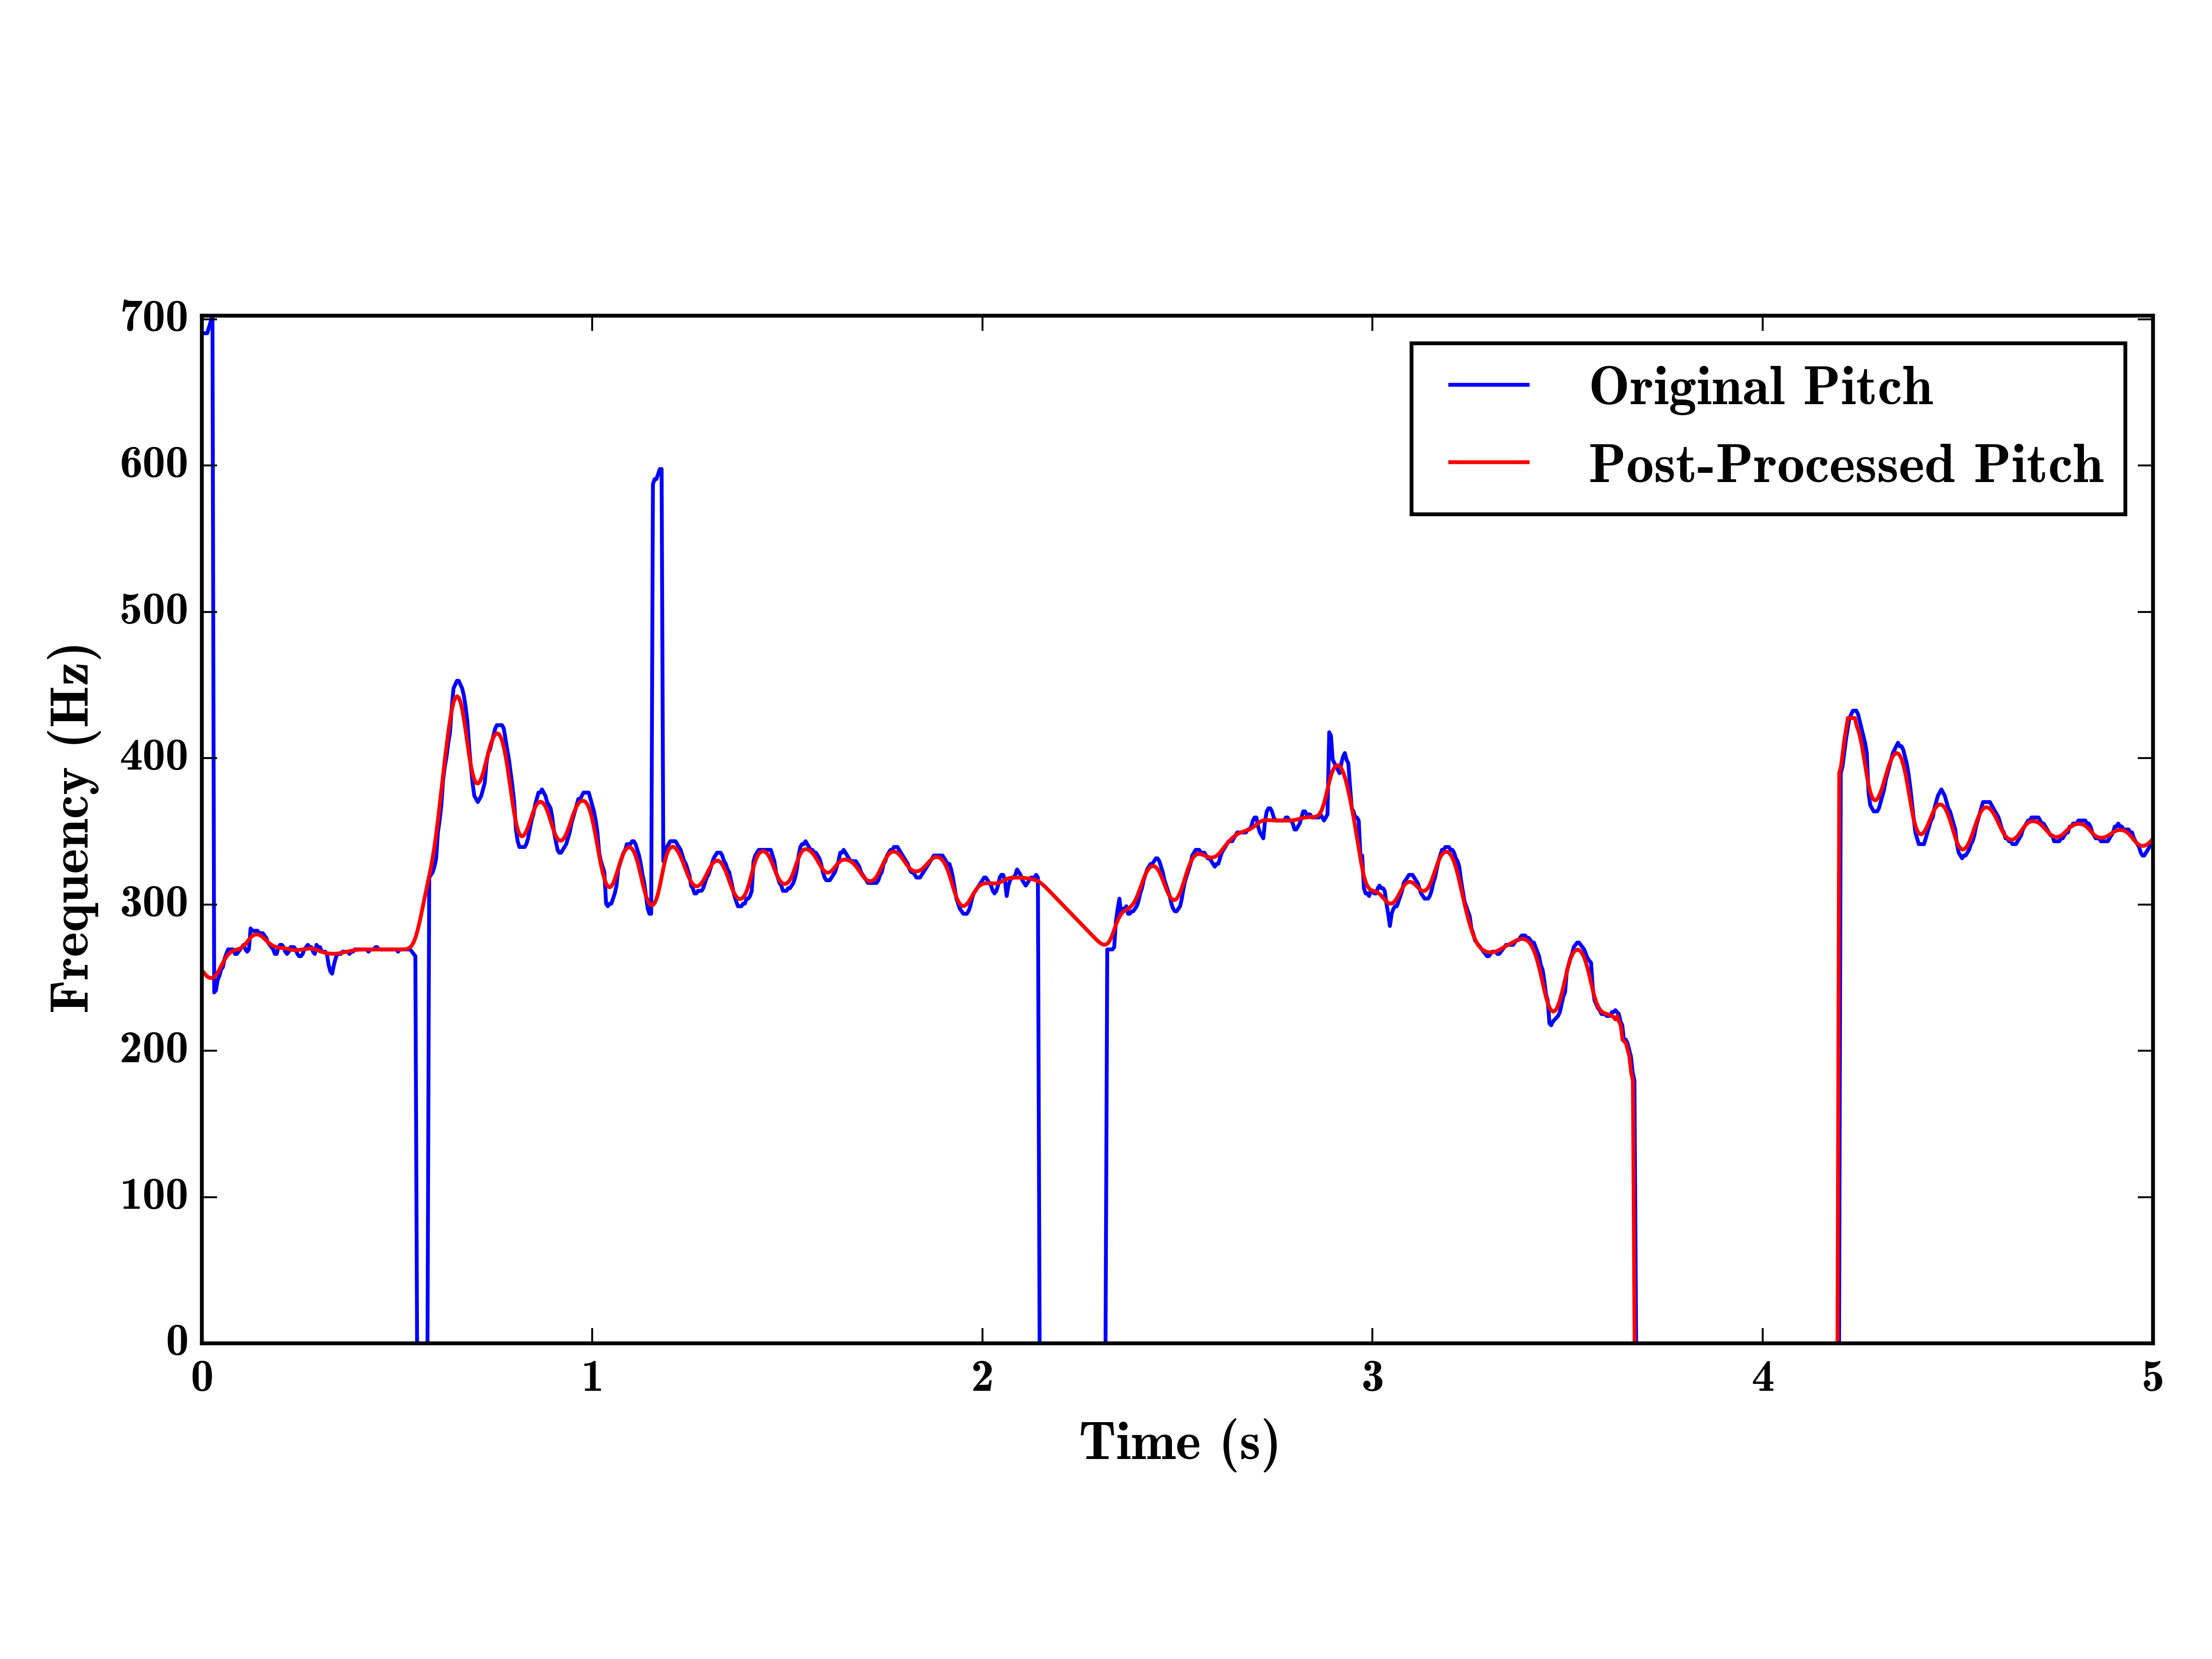
\includegraphics[width=\figSizeHundred]{ch05_preprocessing/figures/smootheningExample.png}
	\end{center}
	\caption[Example of a post-processed predominant pitch segment]{Example of a pitch segment before and after post-processing, which involve median filtering, Gaussian filtering and interpolation of the short unvoiced regions.}
	\label{fig:smoothening_example}
\end{figure}

This processing step aims to remove the spurious pitch jumps lasting over a few frames and to smooth the pitch contours. We start by performing a median filtering on the estimated pitch contour. The window length chosen for median filtering is 50\,ms. Subsequently, to smooth the pitch contour we apply a low-pass filtering by using a Gaussian window. The window size and the standard deviation of the Gaussian window is set to 50\,ms and 10\,ms, respectively. In~\figref{fig:smoothening_example} we show an example of a pitch segment before and after applying median filtering and Gaussian smoothening. We see that the spurious pitch jumps are removed and the pitch contour appears smooth.


\subsubsection{Pitch Interpolation}
\label{sec:data_processing_pitch_interpolation}

In the rendition of melodic phrases in \gls{iam}, there are often unvoiced segments lasting over a small time interval. These unvoiced segments may either correspond to short breath-pauses taken by the vocalists or to the consonants in the lyrics, which are unvoiced in nature. These short unvoiced segments pose a difficulty in the computation of melodic similarity since they do not exist in all the occurrences of a melodic phrase. In such situations assignment of a meaningful numerical value to these unvoiced melodic regions is desired. Therefore, in order to avoid the complexities arising from these unvoiced melodic segments, we interpolate these regions. We perform a linear interpolation across all the unvoiced segments that last for less than 300\,ms. An example of an interpolated unvoiced segment is shown in~\figref{fig:smoothening_example}, between time range of 0 to 1\,s, and 2 to 3\,s.

\subsubsection{Pitch Resampling}
\label{sec:data_processing_pitch_resampling}

An optimal sampling rate of the predominant pitch might depend on the particular computational task under study. For tasks such as analysis of melodic ornaments in \gls{iam}, a high sampling rate might be desired, whereas, for computationally complex tasks such as melodic pattern discovery and search, a sampling rate as low as possible but sufficient to capture melodic nuances might be preferred. In order to avoid predominant melody computation for different sampling rates used across experiments, we resample the predominant melody contours extracted once at a high sampling rate. Pitch contours are decimated to a lower sampling rate by simply downsampling them by an integer factor. The downsampling factor is decided based on the sampling rate used in a particular experiment.

Note that, not all the post-processing steps described in this section are employed in all the experiments. The description of the specific methods in the subsequent chapters will contain details about the post-processing steps used in their respective experiments.


\subsection{Melody Representation} 
\label{sec:pre_processing_melody_representation}

\subsubsection{Hertz to Cent Conversion}
\label{sec:data_processing_cent_conversion}

The perception of melodic intervals for human beings is logarithmic in nature with respect to pitch (or fundamental frequency in Hz). Thus, in order for the pitch representation to be musically meaningful, we convert the estimated predominant pitch values from Hertz to Cents (logarithmic scale) following the equation below.

\begin{equation}
\label{eq:hertz_to_cent_conversion}	
\pitchCents_i = 1200~\log_2\left(\frac{\pitchHz_i}{f_r}\right) ,
\end{equation}

\noindent where $\pitchHz_i$ is the $i^\mathrm{th}$ sample of the predominant pitch in Hertz-scale, $\pitchCents_i$ is the $i^\mathrm{th}$ sample of the predominant pitch in Cent-scale, $f_r$ is the reference tuning frequency which typically in the case of western popular (or even classical) music is set to an integer multiple or sub-multiple of 440\,Hz. We consider $f_r=55$\,Hz, although as we will notice in the next section that this choice is inconsequential.
  

\subsubsection{Tonic Normalization}
\label{sec:tonic_normalization}

As described in~\secref{sec:melody_in_iam} and in~\secref{sec:data_preprocessing_tonic_identification}, in a performance of \gls{iam}, the tonic pitch of the lead performer serves as the reference frequency. Every lead artist chooses a tonic pitch, using which the \gls{tanpura} and the rest of the instruments are tuned. To analyze a melody in the tonal context established by the tonic pitch in a recording ($\toniRec$), we normalize the predominant pitch by this frequency. We perform this normalization by considering the reference frequency $f_r=\toniRec$ in \eqnref{eq:hertz_to_cent_conversion}, which is estimated for every recording using \acrshort{tonicid_justin} method~(\secref{sec:pre_processing_tonic_identification_summary}).


\section{\titlecap{\glsentrytext{nyas} \glsentrytext{svara} Segmentation}}
\label{sec:pre_processing_nyas_segmentation}

Musical melodies contain hierarchically organized events that follow a specific grammar~\citep{Patel07BOOK}. Some of these events are musically more salient than others and act as melodic landmarks. Cadential notes in classical Western music~\citep{GroveCadence} or \gls{karvai} regions in Carnatic music~\citep{sambamoorthy:1998} are examples of such landmarks. While some of these landmarks can be identified based on a fixed set of rules, others do not follow any explicit set of rules and are learned implicitly by a musician through years of music training. A computational analysis of these landmarks can discover some of these implicitly learned rules and help in developing musically aware tools for music exploration, understanding and education. 

Occurrence of a \gls{nyas} in Hindustani music melodies is an example of such a melodic landmark that we investigate in this section. A detailed description of \gls{nyas} is provided in \secref{sec:melody_in_iam}. Typically, occurrence of a \gls{nyas} delimits melodic phrases, which constitute one of the most important characteristic of a \gls{raga}. Analysis of \gls{nyas} is thus a crucial step towards the melodic analysis of Hindustani music. In particular, automatically detecting occurrences of \gls{nyas} (from now on referred as \gls{nyas} segments) will aid in melody segmentation, which is a crucial step in melodic phrase discovery. However, detection of \gls{nyas} segments is a challenging computational task, as the prescriptive definition of \gls{nyas} is very broad, and there are no fixed set of explicit rules to quantify this concept~\citep[p. 73]{Dey2008}. It is through rigorous practice that a seasoned artist acquires perfection in the usage of \gls{nyas}, complying with the \gls{raga} grammar and exploring creativity through improvisation at the same time. 


\begin{figure}
	\begin{center}
		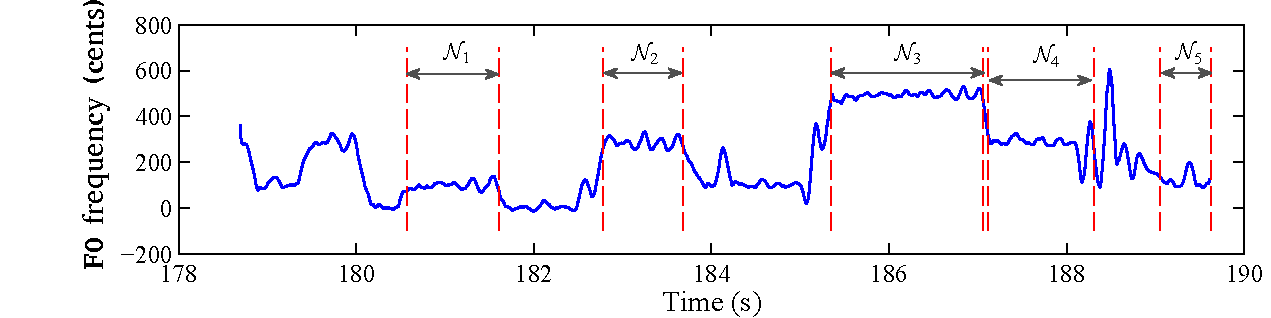
\includegraphics[width=\figSizeHundred]{ch05_preprocessing/figures/NyasFragmentChallenge.pdf}
	\end{center}
	\caption[Fragment of a pitch contour showing \gls{nyas} segments]{Fragment of a pitch contour showing \gls{nyas} segments denoted by $\nSvara_i$ ($i={1...5}$)}
	\label{fig:nyas_segments_example}
\end{figure}

From a computational perspective, the detection of \gls{nyas} segments is challenging due to the variability in segment length, melodic characteristics and the different melodic contexts in which \gls{nyas} is rendered. To illustrate this point we show a fragment of pitch contour in~\figref{fig:nyas_segments_example}, annotated with \gls{nyas} segments denoted by $\nSvara_i$ ($i={1...5}$). We see that the \gls{nyas} segment length is highly varied, where $\nSvara_5$ is the smallest \gls{nyas} segment (even smaller than many non-\gls{nyas} segments) and $\nSvara_3$ is the longest \gls{nyas} segment. In addition, pitch contour characteristics also vary a lot due to the presence of \gls{alankar} (\secref{sec:melody_in_iam}). The pitch characteristics of a segment depend on the \gls{raga} and scale degree of the \gls{nyas}, and adds further complexity to the task~\citep{Bagchee1998}. For example, in~\figref{fig:nyas_segments_example}, $\nSvara_1$ and $\nSvara_3$ have a small pitch deviation from the mean \gls{svara} frequency, whereas, $\nSvara_2$ and $\nSvara_4$ have a significant pitch deviation (close to 100\,cents in $\nSvara_5$). Large pitch deviations also pose a challenge in segmentation process. Furthermore, melodic context such as the relative position with respect to a non-voiced or long melodically constant region plays a crucial role in determining a \gls{nyas} segment. Because of these factors the task of \gls{nyas} segment detection becomes challenging and requires sophisticated learning techniques along with musically meaningful domain specific features.

In the computational analysis of \gls{iam}, \gls{nyas} segment detection has not received much attention in the past. To the best of our knowledge, only one study with the final goal of spotting melodic motifs has indirectly dealt with this task~\citep{Ross2012}. In it, the authors considered performances of a single \gls{raga} and focused on a very specific \gls{nyas} \gls{svara}, corresponding to a single scale degree: the fifth with respect to the tonic, Pa \gls{svara}. This \gls{svara} is considered as one of the most stable \glspl{svara}, and has minimal pitch deviations. Thus, focusing on it oversimplified the methodology developed in~\cite{Ross2012} for \gls{nyas} segment detection. Note that the concept of landmark has been used elsewhere, with related but different notions and purposes. That is the case with time series similarity~\citep{Perng00ICDE}, speech recognition~\citep{Jansen08JASA,Chen12ICASSP}, or audio identification~\citep{Duong13ICASSP}.

In this section, we describe our method for detecting occurrences of \gls{nyas} \gls{svara} in Hindustani music melodies. The description is based on our work presented in~\cite{gulati2014Landmark}. The method consists of two main steps: segmentation based on domain knowledge, and segment classification-based on a set of musically motivated pitch contour features. There are three main reasons for selecting this approach over a standard pattern detection technique (for example \gls{dtw}). First, the pitch contour of a \gls{nyas} segment obeys no explicit patterns, hence, the contour characteristics have to be abstracted. Second, information regarding the melodic context of a segment can be easily interpreted in terms of discrete features. Third, we aim to measure the contribution of a specific feature in the overall classification accuracy (for example, if contour variance and length are the most important features for the classification). This is important in order to corroborate the results obtained from such data driven approaches with that from musicological studies. In the subsequent sections we first describe our method~(\secref{sec:pre_processing_nyas_id_method}), present the methodology used for evaluation~(\secref{sec:pre_processing_nyas_segmentation_experimental_setup}), discuss the results and summarize our findings~(\secref{sec:preprocessing_nyas_segmentation_results_and_discussion}).

\subsection{Method}
\label{sec:pre_processing_nyas_id_method}

The block diagram of the proposed method for \gls{nyas} segmentation is shown in~\figref{fig:bd_nyas_segmentation}. It consists of four main processing blocks: predominant pitch estimation and representation, segmentation, feature extraction, and segment classification and fusion. These processing blocks are described in the following sections.

\begin{figure}
	\begin{center}
		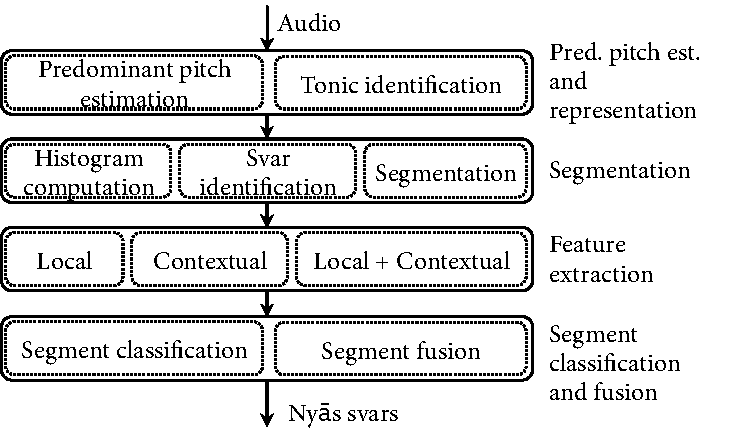
\includegraphics[width=\figSizeEightyFive]{ch05_preprocessing/figures/BlockDiagramNyasSegmentation.pdf}
	\end{center}
	\caption{Block diagram of the proposed approach for \gls{nyas} segmentation.}
	\label{fig:bd_nyas_segmentation}
\end{figure}

\subsubsection{Predominant Pitch Estimation and Representation}

To estimate pitch of the predominant melodic source we use the procedure described in~\secref{sec:data_preprocessing_predominant_melody_estimation} with the same set of parameters. We do not perform any post-processing on the estimated pitch contours. Pitch estimated in Hertz is converted to Cent-scale and is normalized by the tonic of the lead artist in the recording as described in~\secref{sec:data_processing_cent_conversion} and \secref{sec:tonic_normalization}. Tonic pitch of an audio recording is estimated using \acrshort{tonicid_justin} method~(\secref{sec:pre_processing_tonic_identification_summary}). 


\subsubsection{Segmentation}
\label{sec:nyas_svara_segmentation_method}

\Gls{nyas} segment is a rendition of a single \gls{svara} and the aim of the segmentation process is to detect the \gls{svara} boundaries. However, \glspl{svara} contain different \glspl{alankar}, where the pitch deviation with respect to the mean \gls{svara} frequency can go roughly up to 200\,cents~(\secref{sec:melody_in_iam}). This characteristic of a \gls{svara} in Hindustani music poses a challenge to segmentation. To illustrate this, in Figure~\ref{fig:nyas_segmentation_illustration} we present an example of a \gls{nyas} segment (between $\timeStamp_1-\timeStamp_9$, centered around mean \gls{svara} frequency $\freqSvara_n=990$\,cents). The pitch deviation in this \gls{nyas} segment with respect to the mean \gls{svara} frequency reaches almost 100\,cents (between $\timeStamp_5-\timeStamp_6$). Note that here the reference frequency, i.e. 0\,cent correspond to the tonic pitch of the lead singer.

\begin{figure}
	\begin{center}
		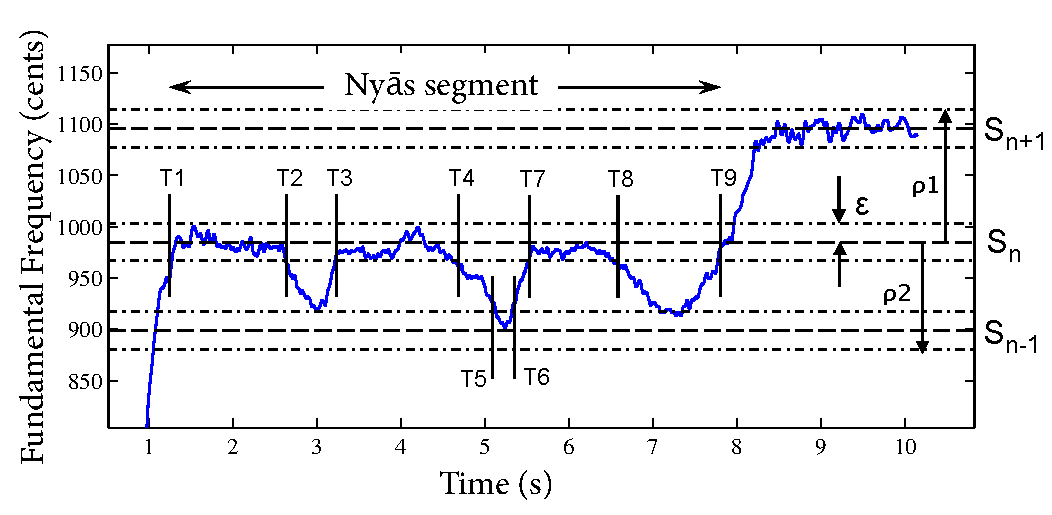
\includegraphics[width=\figSizeNinety]{ch05_preprocessing/figures/NyasSegmentationMethod.pdf}
	\end{center}
	\caption[Illustration of \gls{nyas} segmentation process]{Fragment of a pitch contour containing a \gls{nyas} segment ($\timeStamp_1-\timeStamp_9$), where $\timeStamp_i$s denote time stamps and $\freqSvara_n$s denote mean \gls{svara} frequencies. The pitch deviation within the \gls{nyas} segment ($\timeStamp_1-\timeStamp_9$) is almost 100\,Cents.}
	\label{fig:nyas_segmentation_illustration}
\end{figure}

We experiment with two different methods for segmenting melodies: \gls{pls}, a classical, generic approach used for the segmentation of time series data~\citep{keogh2004segmenting}, and our proposed method, which incorporates domain knowledge to facilitate the detection of \gls{nyas} boundaries. For \gls{pls} we use a bottom-up segmentation strategy as described by~\cite{keogh2004segmenting}. Bottom-up segmentation methods involve computation of residual error incrementally for each sample of time series. When the residual error satisfies a pre-defined criterion a new segment is created. Out of the two typical criteria used for segmentation, namely average and maximum error, we choose the latter because, ideally, a new segment should be created as soon as the melody progresses from one \gls{svara} to the other. In order to select the optimal value of the allowed maximum error, which we denote by $\maxErrorPLS$, we iterated over four different values and chose the one which resulted in the best performance. Specifically, for $\maxErrorPLS=\lbrace 10, 25, 50, 75\rbrace$, $\maxErrorPLS=75$\,cents yielded the best performance. We rejected $\maxErrorPLS\geq 100$\,cents in early experimentation stages because few \glspl{svara} of a \gls{raga} are separated by an interval of 100\,Cents and, therefore, the segmentation output was clearly unsatisfactory.

To make the segmentation process robust to pitch deviations, we propose a method based on empirically-derived thresholds. Unlike \gls{pls}, our proposed method computes a pitch histogram and uses that to estimate mean \gls{svara} frequencies before the computation of residual error. This allows us to compute the residual error with respect to the mean \gls{svara} frequency instead of computing it with respect to the previous segment boundary, as done in \gls{pls}. In this way our proposed method utilizes the fact that the time series being segmented is a pitch contour where the values of the time series hover around mean \gls{svara} frequencies. The mean \gls{svara} frequencies for an excerpt are estimated as the peaks of the histogram computed from the estimated pitch values. An octave folded pitch histogram is computed using a 10\,cent resolution and subsequently smoothened using a Gaussian window with a variance of 15\,cents. Only the peaks of the normalized pitch histogram which have at least one peak-to-valley ratio greater than 0.01 are considered as \gls{svara} locations. As peaks and valleys we simply take all local maximas and minimas over the whole histogram. In~\figref{fig:pitch_histogram_nyas_segmentation} we show an example of an octave folded normalized pitch histogram used for estimating mean \gls{svara} frequencies. The estimated mean \gls{svara} frequencies are indicated by circles. We also notice that the pitch values corresponding to a \gls{svara} span a frequency region and not a single value.


\begin{figure}
	\begin{center}
		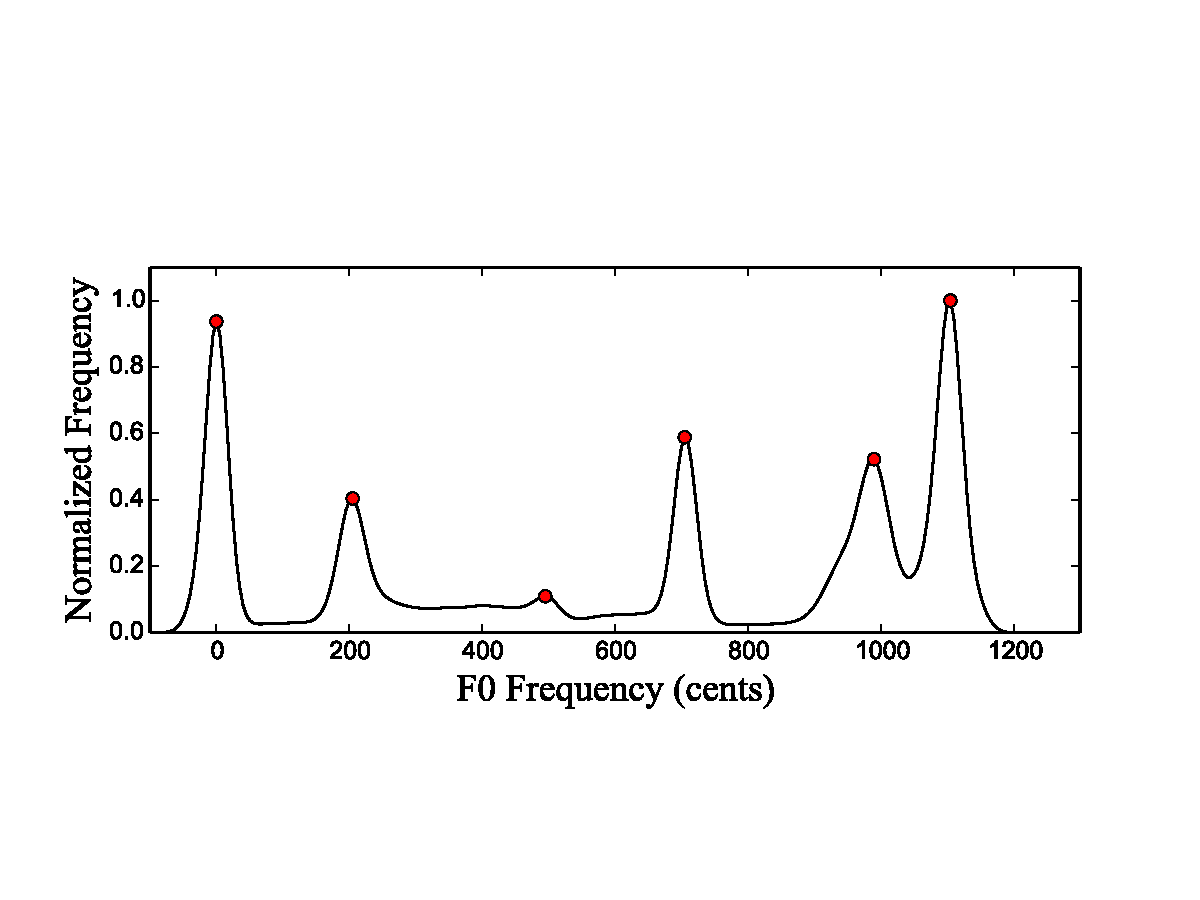
\includegraphics[width=\figSizeNinety]{ch05_preprocessing/figures/swarOnHistogramForNyasSegmentation.pdf}
	\end{center}
	\caption[Example of a normalized octave folded pitch histogram]{Normalized octave folded pitch histogram used for estimating mean \gls{svara} frequencies. Estimated mean \gls{svara} frequencies are indicated by circles.}
	\label{fig:pitch_histogram_nyas_segmentation}
\end{figure}

After we estimate mean frequencies of all the \glspl{svara} in a piece, we proceed with their refinement. For the $n$-th \gls{svara} $\freqSvara_n$, we search for contiguous segments within a deviation of $\awdErrorNyas$ from $\freqSvara_n$, that is, $\vert \freqSvara_n-\pitchCents_i \vert < \awdErrorNyas$, for~$i\in[1,N]$, where $\pitchCents_i$ is the fundamental frequency value (in cents) of the $i$-th sample of a segment of length $N$. In Figure~\ref{fig:nyas_segmentation_illustration}, this corresponds to segments $[\timeStamp_1,\timeStamp_2]$, $[\timeStamp_3,\timeStamp_4]$, and $[\timeStamp_7,\timeStamp_8]$.

Next, we concatenate two segments $[\timeStamp_a,\timeStamp_b]$ and $[\timeStamp_e,\timeStamp_f]$ if two conditions are met:
\begin{enumerate}
	\item $\pitchCents_i-\freqSvara_n < \maxErrorNyas_1$ and $\freqSvara_n-\pitchCents_i < \maxErrorNyas_2$, for $i\in[\timeStamp_b,\timeStamp_e]$, where $\maxErrorNyas_1 = \freqSvara_{n+1}-\freqSvara_n + \awdErrorNyas$ and $\maxErrorNyas_2 = \freqSvara_n-\freqSvara_{n-1} + \awdErrorNyas$. 
	\item $\timeStamp_c-\timeStamp_d < \timeTshldNyas$, where $\timeTshldNyas$ is a temporal threshold and $[\timeStamp_c,\timeStamp_d]$ is a segment between $\timeStamp_b, \timeStamp_e$ such that $\vert \freqSvara_m-\pitchCents_i\vert <\awdErrorNyas$ for $i\in[\timeStamp_c,\timeStamp_d]$ for $m\in [{n-1}, {n+1}]$ and $m \neq n$.
\end{enumerate}

In simple terms, we concatenate two segments if the fundamental frequency values between them do not deviate a lot (less than $\maxErrorNyas_1$ and $\maxErrorNyas_2$) and the time duration of the melody in close vicinity (less than $\awdErrorNyas$) of neighboring \glspl{svara} is not too large (less than $\timeTshldNyas$). We repeat this process for all \gls{svara} locations. In our experiments, we use $\awdErrorNyas = 25$\,cents and $\timeTshldNyas=50$\,ms, which were empirically obtained. Notice that we can already derive a simple binary flatness measure $\binFlatNyas$ for $[\timeStamp_a, \timeStamp_b]$, $\binFlatNyas=1$ if $\vert \freqSvara_n-\pitchCents_i \vert< \awdErrorNyas$ for $i \in [\timeStamp_a, \timeStamp_b]$ for any $n$ and $\binFlatNyas=0$ otherwise. 

\subsubsection{Feature Extraction}
\label{sec:pro_processing_nyas_segmentation_feature_extraction}

We extract musically motivated melodic features for segment classification, which resulted out of discussions with musicians. For every segment obtained following the process mentioned above, three sets of melodic features are computed: local features~(\acrshort{nyas_local_feature}), which capture the pitch contour characteristics of the segment, contextual features~(\acrshort{nyas_context_feature}), which capture the melodic context of the segment, and a third set combining both of them~(\acrshort{nyas_local_feature}+\acrshort{nyas_context_feature}) in order to analyze if they complement each other. Initially, we considered 9 local features and 24 contextual features:

\begin{description}
	\item[Local Features:] segment length, mean and variance of the pitch values in a segment, mean and variance of the differences in adjacent peak locations of the pitch sequence in a segment, mean and variance of the peak amplitudes of the pitch sequence in a segment, temporal centroid of the pitch sequence in a segment normalized by its length, and the above-mentioned flatness measure $\binFlatNyas$ (we use the average segmentation error for the case of \gls{pls}).
	\item[Contextual Features:] segment length normalized by the length of the longest segment within the same breath phrase\footnote{Melody segment between consecutive breaths of a singer. We consider every unvoiced segment (i.e.,~a value of 0 in the pitch sequence) greater than 100\,ms as breath pause.}, segment length normalized by the length of the breath phrase, length normalized with the length of the previous segment, length normalized by the length of the following segment, duration between the ending of the segment and succeeding silence, duration between the starting of the segment and preceding silence, and all the local features of the adjacent segments.
\end{description}

However, after preliminary analysis, we reduced these features to 3 local features and 15 contextual features. As local features we selected length, variance, and flatness measure ($\binFlatNyas$). As contextual features we selected all of them except the local features of the posterior segment. This feature selection was done manually, performing different preliminary experiments with a subset of the data, using different combinations of features and selecting the ones that yielded the best accuracies.

\subsubsection{Classification and Segment Fusion}

Each segment obtained in~\secref{sec:nyas_svara_segmentation_method} is classified into \gls{nyas} or non-\gls{nyas} based on the extracted features described in~\secref{sec:pro_processing_nyas_segmentation_feature_extraction}. To demonstrate that the predictive power of the considered features is generic and independent of a particular classification scheme, we employ five different algorithms exploiting diverse classification strategies~\citep{Hastie09BOOK}: \gls{tree}, \gls{knn}, \gls{nb}, \gls{lr}, and \gls{svm} with a radial basis function kernel. We use the implementations available in scikit-learn~\citep{scikitlearn}, version 0.14.1. We use the default set of parameters with few exceptions in order to avoid over-fitting and to compensate for the uneven number of instances per class. Specifically, we set \texttt{min\_samples\_split=10} for \acrshort{tree}, \texttt{fit\_prior=False} for \gls{nb}, \texttt{n\_neighbors=5} for \gls{knn}, and for \gls{lr} and \gls{svm} \texttt{class\_weight=`auto'}.

For out-of-sample testing we implement a cross-fold validation procedure. We split the dataset into folds that contain an equal number of \gls{nyas} segments, the minimum number of \gls{nyas} segments in a musical excerpt. Furthermore, we make sure that no instance from the same artist and \gls{raga} is used for training and testing in the same fold.

After classification, boundaries of \gls{nyas} and non-\gls{nyas} segments are obtained by merging all the consecutive segments with the same segment label. During this step, the segments corresponding to the silence regions in the melody, which were removed during classification, are regarded as non-\gls{nyas} segments.

\subsection{Experimental Setup}
\label{sec:pre_processing_nyas_segmentation_experimental_setup}

\subsubsection{Music Collection and Annotations}

For evaluation of this task we use the \gls{nyas} dataset \acrshort{nds_cm} as described in~\secref{sec:corpus_nyas_dataset}. As explained, this dataset contains both commercially released polyphonic music recordings and in-house monophonic recordings. As melodic characteristics of a \gls{nyas} segment might depend on the artist and the chosen \gls{raga}, the dataset includes performances by 8 artists in 16 different \glspl{raga} to ensure diversity and representativeness.

\subsubsection{Evaluation Measures and Statistical Significance}

We evaluate two tasks, \gls{nyas} segment boundary annotation, and \gls{nyas} and non-\gls{nyas} segment label annotation. For the evaluation of \gls{nyas} boundary annotations we use hit rates as in a typical music structure boundary detection task~\citep{Ong05ICMC}. While calculating hit rate, segment boundaries are considered as correct if they fall within a certain threshold of a boundary in the ground-truth annotation. Using matched hits, we compute standard precision, recall, and F-score for every fold and average them over the whole dataset. The choice of a threshold however depends on the specific application. Due to the lack of scientific studies on the just noticeable differences of \gls{nyas} \gls{svara} boundaries, we computed results using an arbitrary selected threshold of 100\,ms. Label annotations are evaluated using standard pairwise frame clustering method as described in~\cite{levy2008structural}. Frames with same duration as threshold value for the boundary evaluation (i.e. 100~ms) are considered while computing precision, recall, and F-score. 

For assessing statistical significance we use the Mann-Whitney U test~\citep{mann1947test} with $\pVal<0.05$ and assuming an asymptotic normal distribution of the evaluation measures. To compensate for multiple comparisons we apply the Holm-Bonferroni method~\citep{holm1979simple}, a powerful method that also controls the so-called family-wise error rate. Thus, we end up using a much more stringent criterion than $\pVal<0.05$ for measuring statistical significance.

\subsubsection{Baselines}

Apart from reporting the accuracies for the proposed method and its variants, we compare against some baseline approaches. In particular, we consider \gls{dtw} together with a \gls{knn} classifier ($K=5$). For every segment, we compute its distance from all other segments and assign a label to it based on the labels of its $K$ nearest neighbors, using majority voting. As the proposed method also exploits contextual information, in order to make the comparison more meaningful, we consider the adjacent segments in the distance computation with linearly interpolated values in the region corresponding to the segment. For comparing with the variant of the proposed method that uses a combination of the local and contextual features, we consider adjacent segments together with the actual segment in the distance computation. As this approach does not consider any features, it will help us in estimating the benefits of extracting musically-relevant features from \gls{nyas} segments. 

In addition, to quantify the limitations of the adopted evaluation measures, we compute a few random baselines. The first one (\acrshort{nyas_randbase1}) is calculated by randomly planting boundaries (starting at 0\,s) according to the distribution of inter boundary intervals obtained using the ground-truth annotations. For each segment we assign the labels `\gls{nyas}' with a a priory probability (same for all excerpts) computed using ground truth annotations of the whole dataset. The second one (\acrshort{nyas_randbase2}) is calculated by planting boundaries (starting at 0\,s) at even intervals of 100\,ms and assigning class labels as in \acrshort{nyas_randbase1}. Finally, the third one (\acrshort{nyas_randbase3}) considers the exact ground-truth boundaries and assigns the class labels randomly as in \acrshort{nyas_randbase1} and \acrshort{nyas_randbase2}. Thus, with \acrshort{nyas_randbase3} we can directly assess the impact of the considered classification algorithms. We found that \acrshort{nyas_randbase2} achieves the best accuracy and therefore, for all the following comparisons we only consider \acrshort{nyas_randbase2}.

%\begin{table} 
%\centering
%\begin{tabular}{ c | c c c }
%\hline\hline
%  		&	\acrshort{nyas_randbase1}	&	\acrshort{nyas_randbase2}	&	\acrshort{nyas_randbase3}\\
%\hline
% 	\gls{nyas} Boundary		&  0.10 & 0.17 &1.0  \\ 
%%\hline 	
%	\gls{nyas} Region		& 0.56 & 0.69 & 0.64 \\
%\hline\hline
%\end{tabular}
%
%\caption{F-scores for \gls{nyas} boundary estimation and \gls{nyas} region
%estimation using random baseline methods. \XXX{J}{S}{Why not adding a row or column in the general results tables??}}
%	\label{tab:randombaseline}
%\end{table}

\subsection{Results and Discussion}
\label{sec:preprocessing_nyas_segmentation_results_and_discussion}

We evaluate two tasks, \gls{nyas} segment boundary annotation, and \gls{nyas} and non-\gls{nyas} segment label annotation. For both the tasks, we report results obtained using two different segmentation methods (\gls{pls} and the proposed segmentation method), five classifiers (\acrshort{tree}, \gls{knn}, \gls{nb}, \gls{lr}, \gls{svm}), and three set of features (local (\acrshort{nyas_local_feature}), contextual(\acrshort{nyas_context_feature}) and local together with contextual (\acrshort{nyas_local_feature}+\acrshort{nyas_context_feature})). In addition, we report results obtained using a baseline method (\acrshort{dtw}) and a random baseline (\acrshort{nyas_randbase2}).

In Table~\ref{tab:nyas_segmentation_boundary_accuracy}, we show the results of \gls{nyas} boundary annotations. First, we see that every variant performs significantly better than the best random baseline. \acrshort{nyas_randbase2} yields an F-score of 0.184 while the worst variant tested reaches 0.248. Next, we see that the proposed method achieves a notably higher accuracy compared to the \acrshort{dtw} baseline. Such difference is found to be statistically significant, with the only exception of the \acrshort{nb} classifier. For a given feature set, the performance differences across classifiers are not statistically significant. The only exceptions are \acrshort{tree} and \acrshort{nb}, which yield relatively poor and inconsistent performances over different feature sets. Therefore, we opted to not consider these two classifiers in the following comparisons. Amongst the feature sets, the performance differences are not statistically significant between \gls{pls} variants (Table~\ref{tab:nyas_segmentation_boundary_accuracy}, top rows), whereas for the case of the proposed segmentation method (Table~\ref{tab:nyas_segmentation_boundary_accuracy}, bottom rows), we find that the local features perform significantly better than the contextual features and their combination does not yield consistent improvements. Finally, we see that the best results are obtained using the proposed segmentation method together with the local features, with a statistically significant difference to its competitors. Furthermore, the worst accuracy obtained using the proposed segmentation method is notably higher than the best accuracy using \gls{pls} method, again with a statistically significant difference.

\begin{table} 
\renewcommand{\arraystretch}{1.25}
\setlength{\tabcolsep}{6pt}
	\begin{centering}
	\begin{tabular}{ c : c : c : c c c c c c }
\tabletop
		& Feat.		&	\gls{dtw} & \acrshort{tree}	 &	\gls{knn} 	&	\gls{nb}		& \gls{lr} 	&	\gls{svm}\\
\tablemid
		\multirow{3}{*}{A} & 	\acrshort{nyas_local_feature}		&  0.356 & 0.407 & 0.447 & 0.248 & 0.449 & 0.453\\ 
		%\hline 	
		&	\acrshort{nyas_context_feature}		& 0.284 & 0.394 & 0.387 & 0.383 & 0.389 & 0.406 \\
		%\hline	
		&	\acrshort{nyas_local_feature}+\acrshort{nyas_context_feature}		& 0.289 & 0.414 & 0.426 & 0.409 &0.432 & 0.437 \\
\tablemid
		\multirow{3}{*}{B} &	\acrshort{nyas_local_feature}		& \textbf{0.524} & 0.672 & \textbf{0.719} & 0.491 & \textbf{0.736} & \textbf{0.749}\\ 
		%\hline 	
		&	\acrshort{nyas_context_feature}		& 0.436 & 0.629 & 0.615 & \textbf{0.641} & 0.621 & 0.673 \\
		%\hline	
		&	\acrshort{nyas_local_feature}+\acrshort{nyas_context_feature}		& 0.446 & \textbf{0.682} & 0.708 & 0.591 & 0.725 & 0.735\\  		
\tablebot		
	\end{tabular}	
	\caption[F-scores for \gls{nyas} boundary detection task]{F-scores for \gls{nyas} boundary detection using \gls{pls} method (A) and the proposed segmentation method (B). Results are shown for different classifiers (\acrshort{tree}, \gls{knn}, \gls{nb}, \gls{lr}, \gls{svm}) and local (\acrshort{nyas_local_feature}), contextual (\acrshort{nyas_context_feature}) and local together with contextual (\acrshort{nyas_local_feature}+\acrshort{nyas_context_feature}) features. \gls{dtw} is the baseline method used for comparison. F-score for the random baseline obtained using \acrshort{nyas_randbase2} is 0.184.}
	\label{tab:nyas_segmentation_boundary_accuracy}
	\par	\end{centering}
\end{table}


In~\tabref{tab:nyas_segmentation_label_accuracies}, we show the results for \gls{nyas} and non-\gls{nyas} label annotations. We can draw similar conclusions as with Table~\ref{tab:nyas_segmentation_label_accuracies}: (1) all the method variants perform significantly better than the random baselines, (2) all the proposed method variants yield significant accuracy increments over the \GLS{dtw} baseline, and (3) no statistically significant differences between classifiers (with the aforementioned exceptions). In the label annotations, unlike the boundary annotations, we find that though the local features perform better than the contextual features, the differences are not statistically significant for all the proposed method variants. Furthermore, we also see that the proposed segmentation method consistently performs better than \gls{pls}. However, the differences are not always statistically significant.

In addition, we also investigate per-class accuracies for the label annotations. We find that the performance for the \gls{nyas} segments is considerably better than the non-\gls{nyas} segments. This could be attributed to the fact that even though the segment classification accuracy is balanced across classes, the differences in segment length of \gls{nyas} and non-\gls{nyas} segments (\gls{nyas} segments being considerably longer than non-\gls{nyas} segments) can result in more number of matched pairs for \gls{nyas} segments.

\begin{table} 
\renewcommand{\arraystretch}{1.25}
\setlength{\tabcolsep}{6pt}
\begin{centering}	
	\begin{tabular}{ c : c : c : c  c  c  c  c  c }
\tabletop
		& Feat.	&	\acrshort{dtw} & \acrshort{tree}	 &	\acrshort{knn} 	&	\acrshort{nb}		& \acrshort{lr} 	&	\acrshort{svm}	\\
\tablemid		
		\multirow{3}{*}{A} &   \acrshort{nyas_local_feature}		& \textbf{0.553} & 0.685 & 0.723 & 0.621 & 0.727 & 0.722	\\
		%\hline         
		&	\acrshort{nyas_context_feature}   		& 0.251 & 0.639 & 0.631  & 0.690 & 0.688 & 0.674	\\
		%\hline 
		& 	\acrshort{nyas_local_feature}+\acrshort{nyas_context_feature}		& 0.389 & 0.694 & 0.693 & 0.708 & 0.722 & 0.706	\\	
		\hline
		\multirow{3}{*}{B} & 	\acrshort{nyas_local_feature}		& 0.546 & \textbf{0.708} & \textbf{0.754} & 0.714 & \textbf{0.749} & \textbf{0.758} \\
		%\hdashline 	
		& 	\acrshort{nyas_context_feature}		&0.281 & 0.671 & 0.611 & 0.697 & 0.689 & 0.697\\
		%\hline	
		& 	\acrshort{nyas_local_feature}+\acrshort{nyas_context_feature}		& 0.332 & 0.672 & 0.710 & \textbf{0.730} & 0.743 & 0.731\\
\tablebot
	\end{tabular}
	\caption[F-scores for \gls{nyas} and non-\gls{nyas} label annotation task]{F-scores for \gls{nyas} and non-\gls{nyas} label annotation task using \gls{pls} method (A) and the proposed segmentation method (B). Results are shown for different classifiers (\acrshort{tree}, \acrshort{knn}, \acrshort{nb}, \acrshort{lr}, \acrshort{svm}) and local (\acrshort{nyas_local_feature}), contextual (\acrshort{nyas_context_feature}) and local together with contextual (\acrshort{nyas_local_feature}+\acrshort{nyas_context_feature}) features. \acrshort{dtw} is the baseline method used for comparison. The best random baseline F-score is 0.153 obtained using \acrshort{nyas_randbase2}. } 
	\label{tab:nyas_segmentation_label_accuracies}
\par \end{centering}
\end{table}


In general, we see that the proposed segmentation method improves the performance over \gls{pls} method in both the tasks, wherein the differences are statistically significant in the former case. Furthermore, the local feature set, when combined with the proposed segmentation method, yields the best accuracies. We also find that the contextual features do not complement the local features to further improve the performance. However, interestingly, they perform reasonably good considering that they only use contextual information.


\subsection{Summary}
\label{ConclusionAndFutureWork}

We described a method for detecting \gls{nyas} segments in melodies of Hindustani music. We divided the task into two broad steps: melody segmentation and segment classification. For melody segmentation we proposed a method which incorporates domain knowledge to facilitate \gls{nyas} boundary annotations. We evaluated three feature sets: local, contextual and the combination of both. We showed that the performance of the proposed method is significantly better compared to a baseline method using standard \gls{dtw} based distance and a \gls{knn} classifier. Furthermore, we showed that the proposed segmentation method outperforms a standard approach based on \gls{pls}. A feature set that includes only the local features was found to perform best. However, we showed that using just the contextual information we could also achieve a reasonable accuracy. This indicates that \gls{nyas} segments have a defined melodic context which can be learned automatically. 


\section{Tani Segmentation}
\label{sec:pre_processing_tani_segmentation}

A concert of Carnatic music typically contains a solo percussion section towards the end of the concert, referred to as \gls{tani} avartanam or \gls{tani} in short. The duration of this section typically varies from 2 to 25\,min depending on the artist and the context. The main percussion instrument in Carnatic music is \gls{mridangam}, which becomes the lead instrument during this section. Along with the \gls{mridangam} there are other percussion instruments often played in \gls{tani} section such as \gls{kanjira} and \gls{ghatam}. Though \gls{mridangam} is a percussion instrument and is basically a kind of a barrel drum, its sound has tonal characteristics. Like the other accompanying instruments in Carnatic music such as \gls{tanpura} and violin, \gls{mridangam} is also tuned at the tonic of the lead artist. Due to the tonal acoustical characteristics of \gls{mridangam} sound, and because of the long duration of \gls{tani} sections, the pitch estimation algorithm detects and tracks pitch contours during the \gls{tani} sections, instead of detecting these sections as non-voiced segments. Notice that the \gls{mridangam} strokes during short (lasting over roughly 1-20 seconds) unvoiced segments such as breath-pauses are correctly detected as non-voiced by the predominant pitch estimation algorithm. This is due to the fact that during such sections the predominant pitch corresponds to the voice, which has significantly higher energy compared to the background percussion signal. 


\begin{figure}
	\begin{center}
		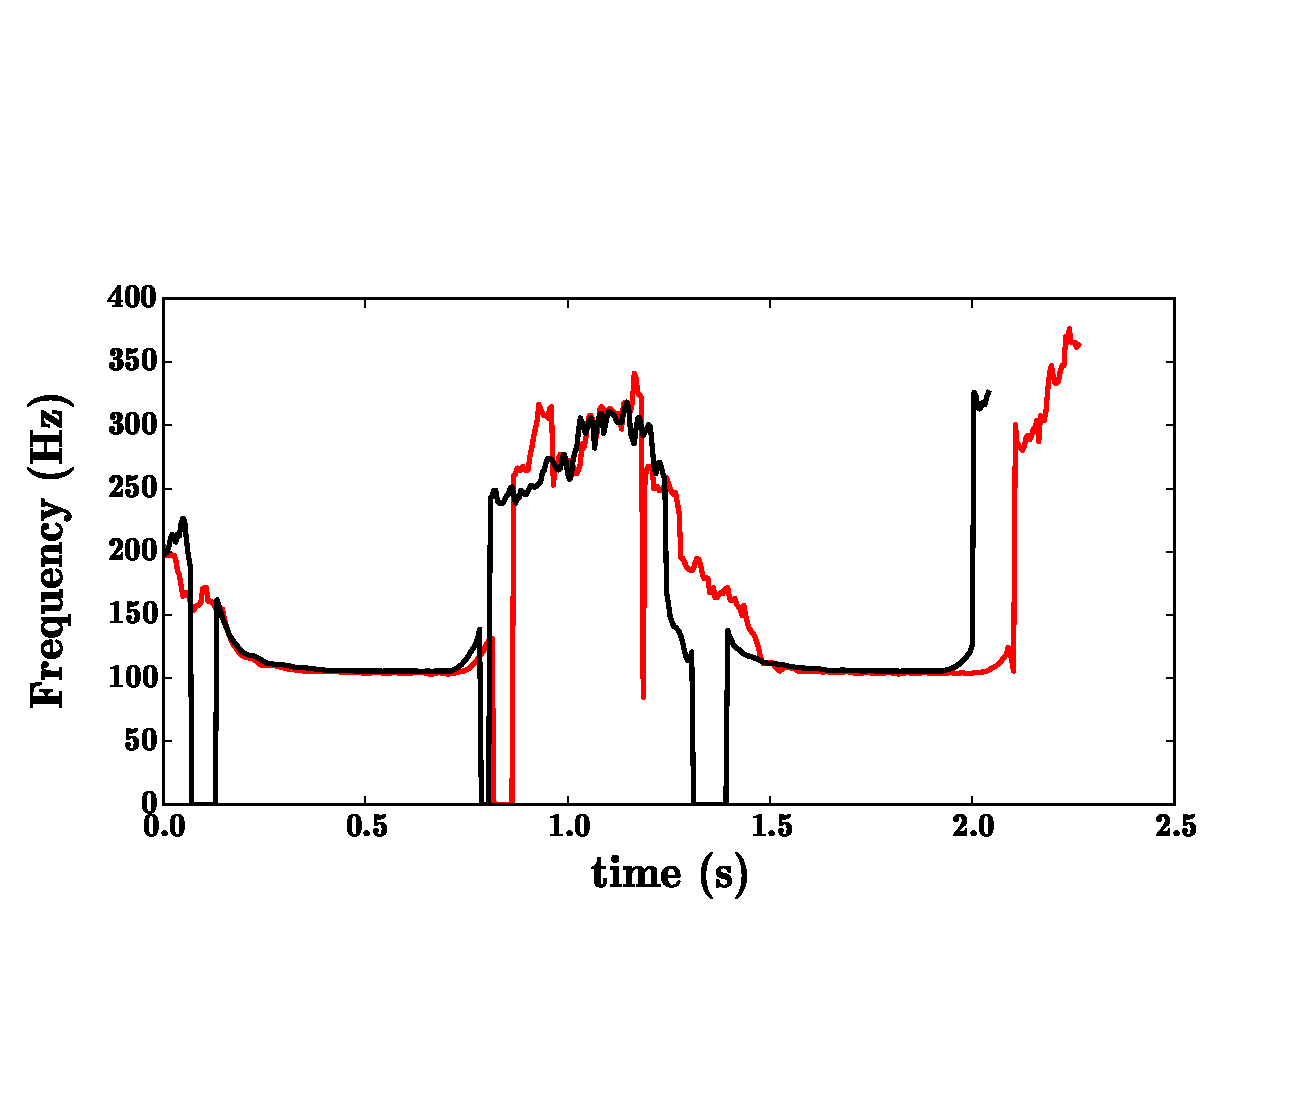
\includegraphics[width=\figSizeNinety]{ch05_preprocessing/figures/taniPatterns.pdf}
	\end{center}
	\caption[Melodic patterns corresponding to the \gls{mridangam} strokes]{Pitch contours of a pair of highly similar melodic patterns corresponding to the \gls{mridangam} strokes in a \gls{tani} section.}
	\label{fig:pitch_pattern_tani}
\end{figure}

Detecting pitch corresponding to the \gls{mridangam} strokes as predominant pitch in the audio poses several challenges in melodic analyses, specifically in the discovery of melodic patterns. Percussion patterns and rhythm cycles contain recurring strokes (or patterns), and therefore, pitch fragments from the \gls{tani} section are frequently discovered as highly similar patterns. An example of a discovered pair of pitch patterns that correspond to \gls{mridangam} strokes is shown in~\figref{fig:pitch_pattern_tani}. We see that the patterns are close to exact repetitions. Since we aim to discover patterns in melodies of \gls{iam} (\chapref{chap:melodic_pattern_processing}), patterns discovered from the \gls{tani} sections are undesired. There can be two approaches to avoid such unwanted patterns in the final output: 1) post-process the discovered pitch patterns and detect if they belong correspond to \gls{mridangam} strokes, 2) discard pitch contours corresponding to the \gls{tani} section in the pre-processing step. We follow the second approach and discard segments of the pitch contours that correspond to the \gls{tani} sections from the input given to the pattern discovery method. Discarding such segments upfront has several advantages. First, detection of the \gls{tani} sections in audio recording appears to be an easier task compared to characterizing pitch contours as belonging to the melody or \gls{mridangam} strokes. This is mainly because of the considerable amount of timbral differences across the sections where melody is present and where it is not. In addition, such computational tasks of classifying an audio segment based on its timbral characteristics is well studied in \gls{mir}~\citep{herrera2003automatic}. In~\figref{fig:spectrogram_of_tani_segment}, we show the spectrogram of a voice section and a \gls{tani} section. We see that the timbral characteristics between the two types of sections are considerably different. Another benefit of discarding the \gls{tani} sections upfront is that it reduces the computational complexity of the pattern discovery task (\gls{tani} sections may last up to 2-25\,minutes). %We therefore detect \gls{tani} sections directly in the audio recordings and discard the pitch segments corresponding to these sections in the pre-processing step.

\begin{figure}
	\begin{center}
		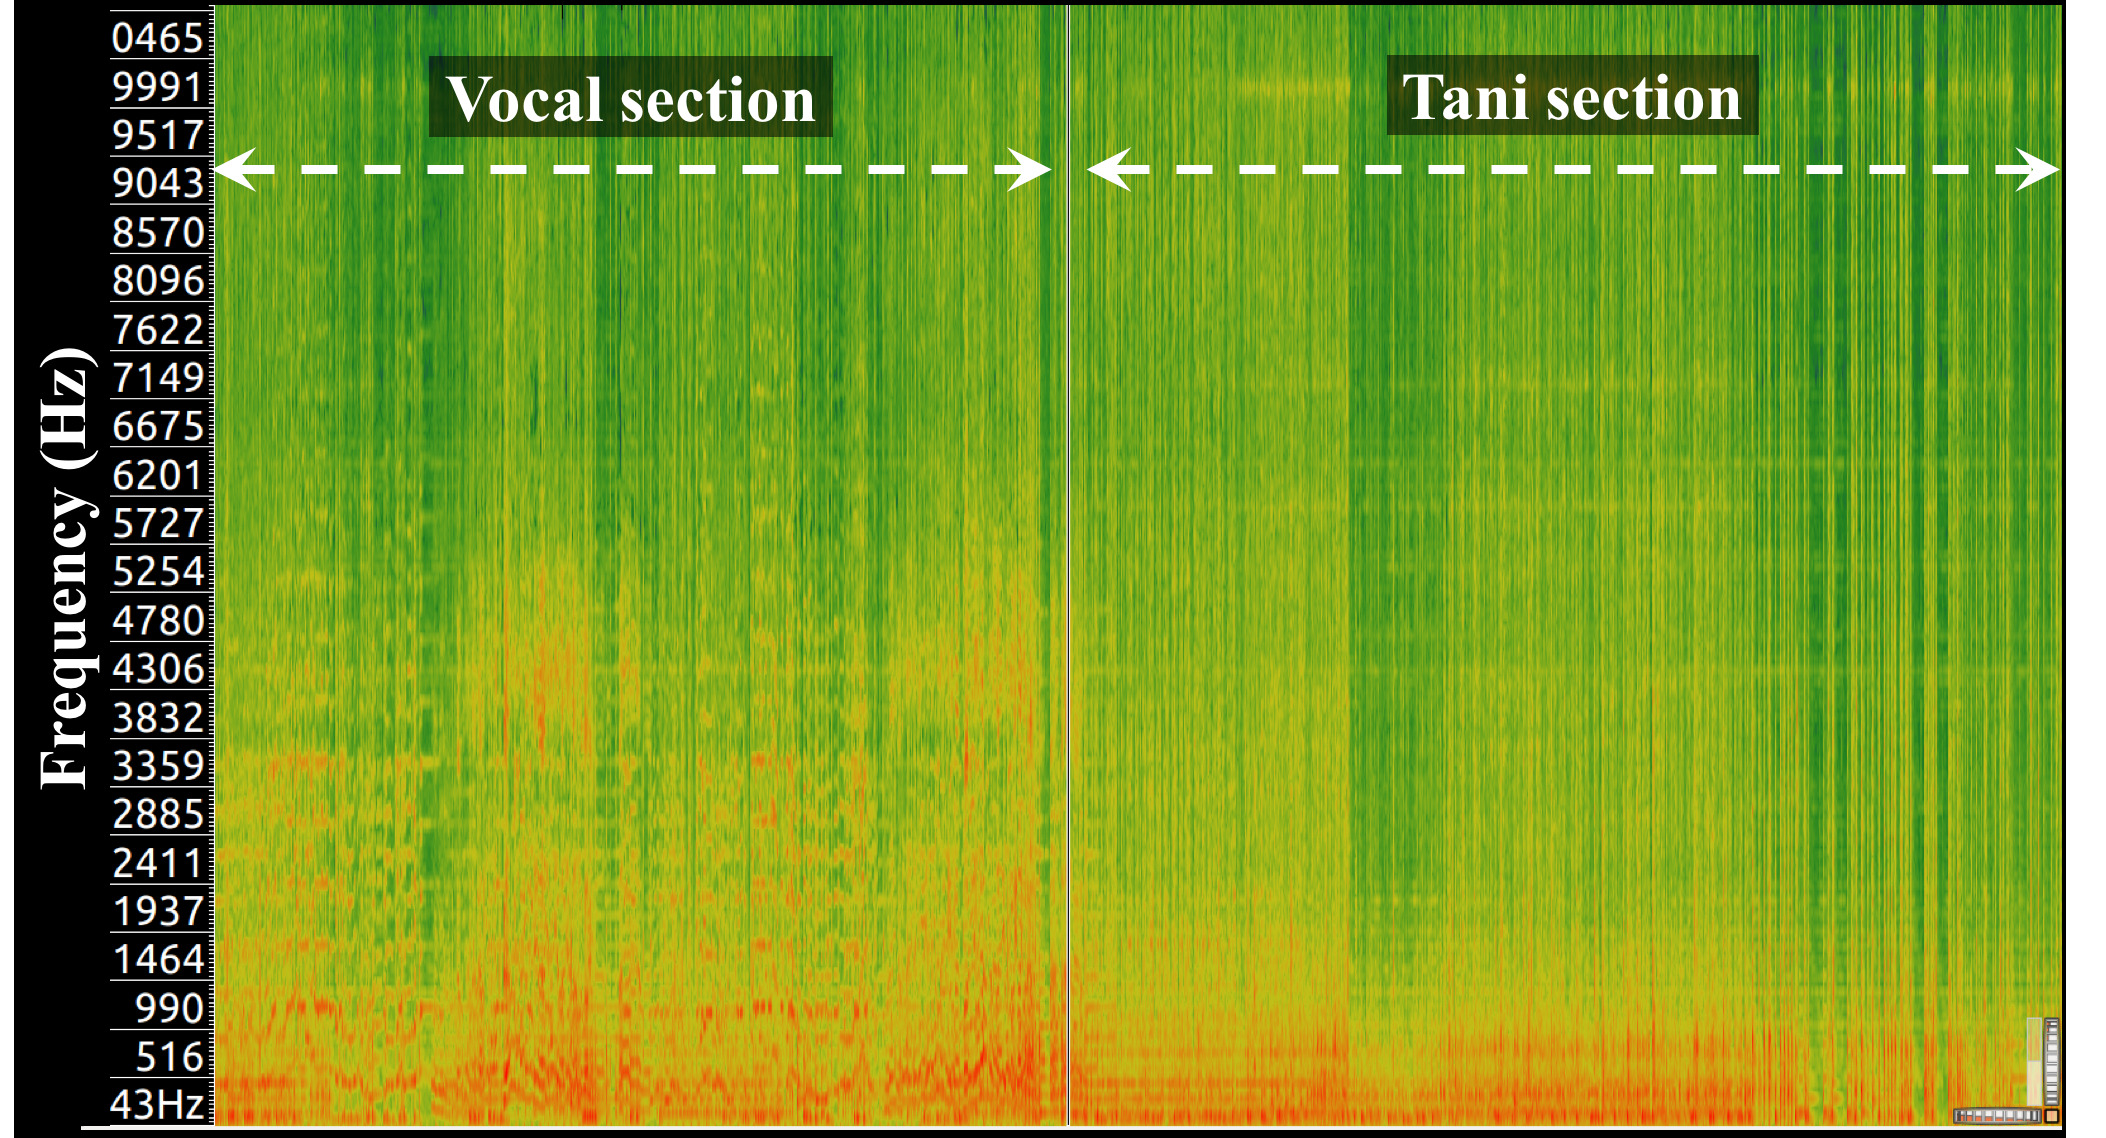
\includegraphics[width=\figSizeEighty]{ch05_preprocessing/figures/spectrogramTani.png}
	\end{center}
	\caption[Illustration of spectrogram a vocal and a \gls{tani} section]{Spectrogram of a voice (with percussion) and a \gls{tani} section in an audio recording of Carnatic music. Spectrogram spans 3\,minutes of audio.}
	\label{fig:spectrogram_of_tani_segment}
\end{figure}

We detect \gls{tani} sections in audio recordings using a classification-based approach. To feed the classifiers we extract 13~\acrshort{mfcc} coefficients, spectral centroid, spectral flatness and pitch salience from the audio signal using Essentia~\citep{essentia} library. We iterate over 23, 46 and 92\,ms frame sizes and chose the one that results in the best classification accuracy. We set the hop size as half the frame size and all other parameters to their default values. Next, we compute the means and the variances of these features over 2\,s non-overlapping segments (sometimes referred to as texture window). For training, we use a labeled audio music dataset containing 1.5~hours of mixed voice and violin recordings and 1.5~hours of solo percussion recordings. To assess the performance of the extracted features, we perform a 10-fold cross-validation procedure and repeat the experiment 10 times. We experiment with five different algorithms exploiting diverse classification strategies~\citep{Hastie09BOOK}: decision trees (\acrshort{tree}), \gls{knn}, \gls{nb}, \gls{lr}, and \gls{svm} with a radial basis function kernel. We use the implementations of the classifiers as available in scikit-learn version~0.14.1~\citep{scikitlearn}. We used the default set of parameters with few exceptions to avoid over-fitting and to compensate for the uneven number of instances per class. We set \texttt{min\_} \texttt{samples\_split=10} for \acrshort{tree}, \texttt{fit\_prior=False} for \gls{nb}, \texttt{n\_neighbors=5} for \gls{knn}, and for \gls{lr} and \gls{svm} \texttt{class\_weight=`auto'}. 

The combination of the frame size of 46\,ms and the \gls{svm} classifier yielded the best performance (96\% accuracy), with no statistically significant difference to the performance with the \acrshort{tree} (95.5\%) and the \gls{knn} (95\%), for the same frame size. We finally chose \gls{knn} because of its low complexity. Detection accuracy of the \gls{tani} sections can be improved further by a simple post-processing step. Since \gls{tani} is a single continuous section in an audio recording, class labels of the texture windows predicted by the classifier can be median filtered to remove the spurious labels lasting over a few frames. This ensures continuity of the class labels across texture windows and avoids short non-voiced regions during the vocal sections being classified as \gls{tani} segments. 

\section{Summary}
\label{sec:preprocessing_summary}

%\XXX{S}{J}{I am finding it difficult to describe the contents of this chapter in a single concept (descriptors or representations). Strictly speaking, referring to nyas segmentation as melodic descriptors is misleading. Its already a higher level analysis. If you have any suggestion to change the way I introduce this chapter or to group these 4 different sections please let me know.}

In this chapter, we described methods to obtain relevant melodic descriptors and melody representations from audio recordings. We presented algorithms used to extract and post-process the predominant pitch from these recordings. To match the tonal context of melodies across performances, the predominant pitch is normalized by the tonic used in the recordings. We presented an exhaustive evaluation of a number of tonic identification approaches, wherein we analyzed and compared their performance on different music material such as Hindustani and Carnatic music, male and female singers, and for instrumental and vocal music. We showed that our multipitch approach consistently outperformed all the other methods. Subsequently, we described our \gls{nyas}-based approach for segmenting melodies in Hindustani music. We saw that a knowledge driven segmentation approach performs better than a generic method for segmenting time-series data. In addition, we showed that our classification-based approach that uses abstracted melodic features performs better than a string matching based method for labeling \gls{nyas} segments. Furthermore, we demonstrated the utility of the context-based melodic features for \gls{nyas} detection task. At the end of the chapter, we explained our methodology for identifying \gls{tani} sections in audio recordings of Carnatic music. We showed that a classification-based approach that uses timbral features can successfully identify \gls{tani} sections with accuracy.

%\COMMENT{Somehow I am not able to write nicely a summary of this chapter. Please let me know if you clearly see what's missing.}
%

 
%\cleartorecto%!TEX root = ../thesis_a4.tex

\chapter{Melodic Pattern Processing: Similarity, Discovery and Characterization}
\label{chap:melodic_pattern_processing}
\chaptermark{Melodic Pattern Processing}

\section{Introduction}
\label{sec:patterns_introduction}

In this chapter, we present our methodology for discovering musically significant melodic patterns in sizable audio collections of \gls{iam}. We address three main computational tasks involved in this process; melodic similarity, pattern discovery and characterization of the discovered melodic patterns. We refer to these different tasks jointly as melodic pattern processing.

\blockcquote[]{schenker1980harmony}{\textit{Only by repetition can a series of tones be characterized as something definite. Only repetition can demarcate a series of tones and its purpose. Repetition thus is the basis of music as an art}}

Repeating patterns are at the core of music. Consequently, analysis of patterns is fundamental in music analysis.  In \gls{iam}, recurring melodic patterns are the building blocks of melodic structures. They provide a base for improvisation and composition, and thus, are crucial to the analysis and description of \glspl{raga}, compositions, and artists in this music tradition. A detailed account of the importance of melodic patterns in \gls{iam} is provided in~\secref{sec:melody_in_iam}. 

%As mentioned before, there are various types of melodic patterns that characterize different aspects of melodies in \gls{iam}. Some of these recurring patterns, referred to as characteristic melodic phrases (\secref{sec:music_background}), are prominent cues used by performers, to establish the identity of a \gls{raga}, and listeners, to identify the \gls{raga} in a music piece. Thus, automatically detecting occurrences of these melodic patterns is key to melodic analyses of \gls{iam}, and a crucial step towards meaningful retrieval and recommendation of \gls{iam}.

%In this chapter we present approaches that address different computational tasks related to patterns in melodies of \gls{iam}. These tasks include computing melodic similarity between two melodic fragments, discovering melodic patterns in large audio music collections, and finally, characterizing discovered melodic patterns. We present relevant work done on these topics in \gls{mir} and highlight their shortcomings and reasons for their inapplicability to melodies in \gls{iam}. We describe our proposed approaches in detail and perform comprehensive evaluations. The description provided in this chapter is primarily based on our work presented in~\cite{gulati_SITIS_2014,gulati_ICASSP2015, gulati_ISMIR_2015,gulati_communities_2016}.

%As mentioned before, one of the key objectives of this dissertation is to extract melodic patterns in sizable audio collections of \gls{iam}. These patterns can then be characterized and used for performing computational tasks such as \gls{raga} recognition~(\chapref{chap:raga_recognition}). 

To recapitulate, from the literature review presented in~\secref{sec:sota_pattern_processing_iam} and \secref{sec:pattern_processin_in_music} we see that the approaches for pattern processing in music can be broadly put into two categories (\figref{fig:types_of_methodologies_for_extraction}). One of the types of approaches perform pattern detection (or matching) and follow a supervised methodology. In these approaches the system knows \textit{a priori} the pattern to be extracted. Typically such a system is fed with exemplar patterns or queries and is expected to extract all of their occurrences in a piece of music or in a music collection. In the context of melodies in \gls{iam}, this would mean that musicians provide examples of melodic patterns, which are then used to retrieve all of their occurrences in an audio collection. Nearly all the methods proposed for pattern processing in \gls{iam} take a supervised approach (\secref{sec:sota_pattern_processing_iam}). Note that this research problem is also addressed to an extent in a related task of \acrfull{qbh} (\secref{sec:query_by_humming}).

\begin{figure}
	\begin{center}
		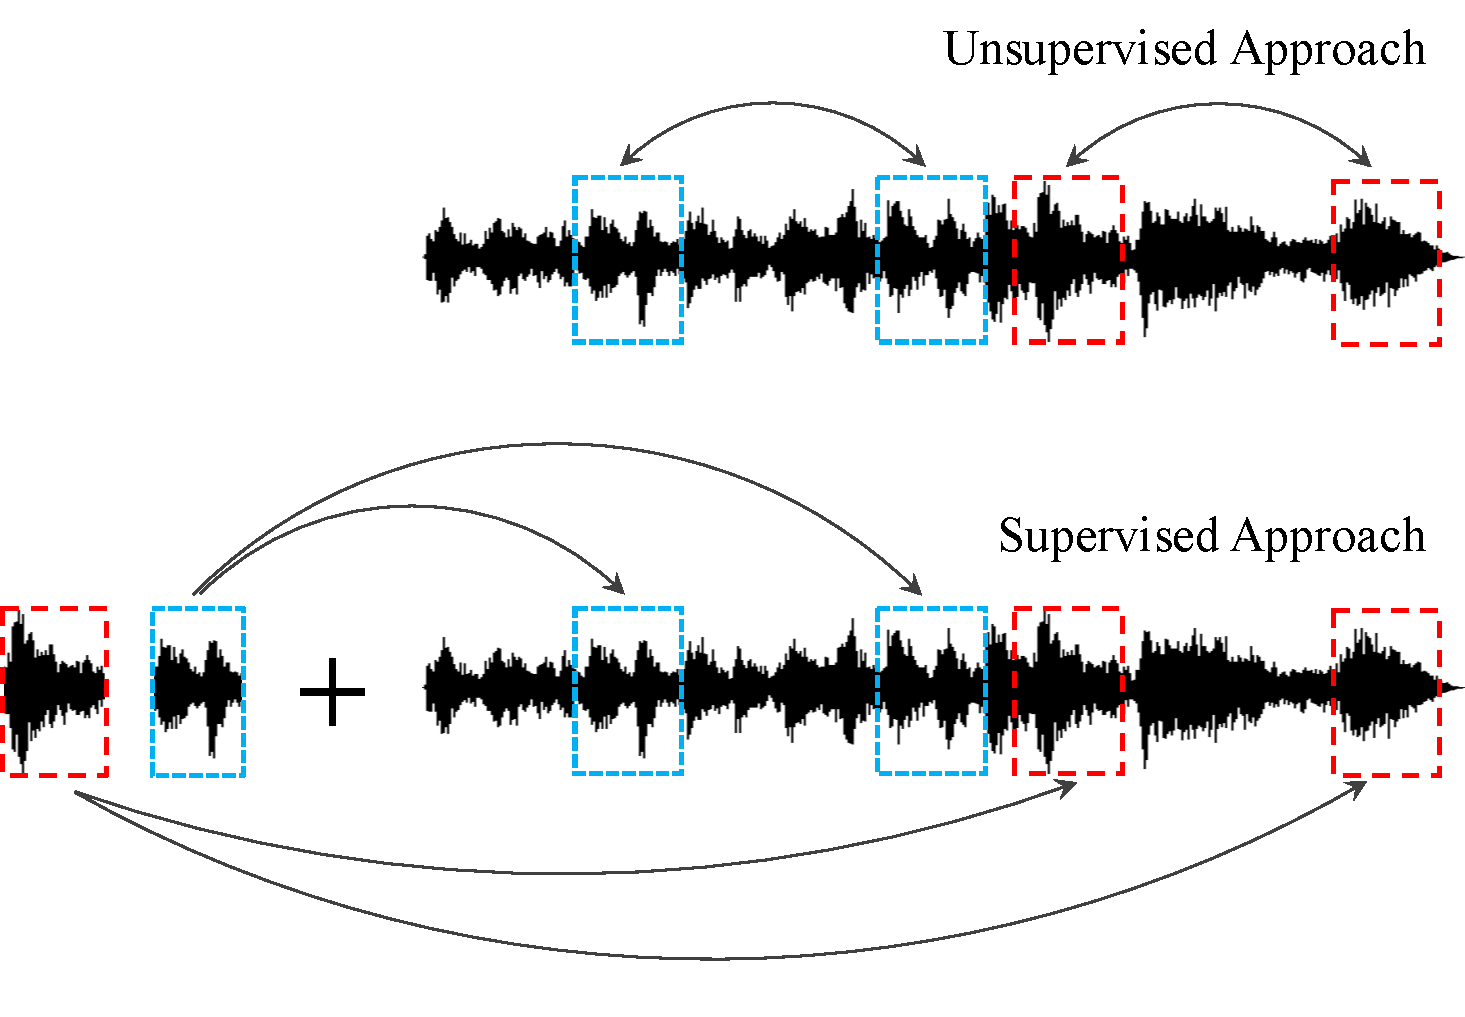
\includegraphics[width=\figSizeEighty]{ch06_patterns/figures/discovery/TwoTypesOfMethodology.pdf}
	\end{center}
	\caption{Two types of approaches for pattern extraction in music recordings.}
	\label{fig:types_of_methodologies_for_extraction}
\end{figure}

We identify several caveats in the supervised methodology described above in the context of pattern processing for melodies in \gls{iam}. We believe that using only a supervised methodology severely limits the potential of a pattern-based melodic analysis in \gls{iam}. This is primarily because of the following reasons:

\begin{itemize}
	\item \textbf{Dataset size:} Manually annotating instances of melodic patterns for hundreds of hours of music is a cumbersome process. Since the task of melodic segmentation and similarity is to an extent subjective, ideally speaking, the annotations should be done by multiple domain experts, which makes this task even more challenging. Thus, building a representative and comprehensive corpus of musically meaningful melodic patterns becomes practically unfeasible. This is clearly evident from the size of the datasets used in the existing studies (\secref{sec:sota_pattern_processing_iam}, \tabref{tab:pattern_processing_iam}). The existing datasets typically comprise only a handful of \glspl{raga}, tens of music pieces, tens of unique number of melodic phrases and a single annotator.

	\item \textbf{Knowledge bias:} The process of annotating melodic patterns in audio recordings of \gls{iam} essentially boils down to marking regions in time where a known melodic phrase (\gls{raga} motif, or \gls{mukhda}) occurs. With long audio recordings (some lasting up to an hour) and improvisatory characteristics of this music, annotating every repeated melodic pattern in the melody (using the concept of parallelism) is close to impossible. This can be attributed to the limited memory of human listeners. Thus, an annotated corpus of melodic patterns suffers from a bias (only the patterns known to an annotator are marked), and does not contain all possible repeating patterns. This is also evident from the datasets used in the existing studies (\secref{sec:sota_pattern_processing_iam}, \tabref{tab:pattern_processing_iam}). The annotated melodic patterns either correspond to \gls{mukhda} phrase or to few well known \gls{raga} motifs. 
	
	\item \textbf{Human errors:} We found that even when expert listeners are annotating known melodic phrases they are susceptible to making errors in judgment. One of the possible reasons we discovered is the influence of the local melodic context on phrase segmentation. In one of the pattern datasets, \acrshort{msds} (\secref{sec:corpus_melodic_similarity_dataset}), we found several instances where many repetitions of the melodic patterns were missed by professional musicians. When these missed instances of the patterns were heard in isolation by the same set of musicians, they were correctly identified. The number of the missed pattern instances was significant, nearly 25\% of the total number of annotated patterns. In our conversations with some of these musicians, they commented that the local melodic context masked these patterns and influenced their segmentation. While this phenomenon is yet to be scientifically studied for \gls{iam}, we at least know that melodic pattern annotations done  by even professional musicians are prone to such errors. 			
\end{itemize}

One way to circumvent the issues enumerated above is to follow an unsupervised methodology for pattern processing~(\figref{fig:types_of_methodologies_for_extraction}). In such an approach a system discovers patterns in the data without any training examples from an expert or a query pattern. In the context of our work, such a system will not require any examples of the annotated melodic patterns from musicians, and thus can be robust to the issues enumerated above. Also, from our literature review presented in~\secref{sec:sota_pattern_processing_iam}, we notice that there are only a few studies that address the task of discovering short-time melodic patterns in audio music collections. Based on these considerations, in this thesis we follow an unsupervised approach for discovering melodic patterns in sizable audio collections of \gls{iam}. 

The discussion above brings us to an interesting question, what do we mean by a melodic pattern given we do not have any example of it provided by an expert? Recall (\secref{sec:background_terminology}), in the scope of this thesis any recurring melodic fragment is considered as a melodic pattern. We believe that since it repeats, it is not just a coincidence, but it has some significance as the artist rendered the same melodic fragment multiple times. It should be noted that by a recurrence we do not mean a numerical repetition of the pitch sequence. By a recurrence in this context we refer to a musical recurrence of a melodic pattern, which can undergo several melodic variations allowed in the music tradition without loosing its musical identity. In addition, we carefully differentiate the term melodic pattern from melodic motif, wherein the latter is used to refer to a musically significant pattern that is characteristic of a \gls{raga} or a composition (\secref{sec:background_terminology}). 

Along with the aforementioned advantages, there are several challenges in following an unsupervised approach for pattern extraction. One of the most challenging aspects of such approaches is its quantitative evaluation. Due to the absence of ground-truth annotations evaluating such approaches becomes difficult. This becomes even more challenging for a data-driven research methodology since the system parameters are often optimized based on the data. After our first study presented in~\cite{gulati_SITIS_2014} on mining melodic patterns, we realized that selecting optimal values of the system parameters is notoriously difficult in a completely unsupervised setup. As a result, we bootstrap our methodology by first improving one of the core processing blocks in this task, the computation of melodic similarity, within a supervised setup. 

This chapter is divided into four sections, each of which focuses on an important aspect related with pattern processing in \gls{iam}. The contents of these sections are:
\begin{itemize}
	\item In \secref{sec:patterns_evaluation_of_similarity_measures}, we address the task of computing melodic similarity. The main objective is to perform an exhaustive evaluation of different methodologies and parameter settings in order to study their influence on the computation of melodic similarity  in \gls{iam}. This section is based on our work presented in~\cite{gulati_ICASSP2015}.
	\item In \secref{sec:patterns_improving_melodic_similarity}, we focus on improving melodic similarity in \gls{iam} by exploiting the culture specific characteristics of the melodies in Carnatic and Hindustani music. This section is based on the study presented in~\cite{gulati_ISMIR_2015}.
	\item In \secref{sec:patterns_melodic_pattern_discovery}, we describe our methodology for discovering melodic patterns in audio music collections of \gls{iam}. This section is largely based on our work presented in~\cite{gulati_SITIS_2014}.
	\item In \secref{sec:patterns_characterization_of_melodic_patterns}, we describe our approach to characterize the discovered melodic patterns in order to identify the ones that correspond to the \gls{raga} motifs. This section is based on our published work in~\cite{gulati_communities_2016}.
\end{itemize}


%################################################################################################################
%########################################### Melodic Similarity Evaluation ######################################
%################################################################################################################


\section{Melodic Similarity: Approaches and Evaluation}
\label{sec:patterns_evaluation_of_similarity_measures}

In this thesis, we regard repeating melodic fragments as melodic patterns. As explained above, the concept of repetition or recurrence in this context is not just a numerical reiteration of exactly the same pitch sequence. But, it is musical in nature, allowing for permitted melodic variations. Thus, the idea of repetition is closely linked to perceptual melodic similarity, which is influenced by several factors including the specificities in a music culture. Our objective in this study is to model this perceptual similarity between short-duration melodic fragments, which will eventually be used for extracting melodic patterns in audio collections of \gls{iam}.

Studying computational models for melodic similarity is particularly interesting in the context of \gls{iam}. This is mainly because this music is inherently improvisatory in nature, and the melodies are largely based around melodic patterns. Due to the melodic improvisation, which is largely governed by \gls{raga} grammar, the surface representation of melodic patterns varies significantly across occurrences. This is specifically true for the characteristic melodic patterns of \glspl{raga} (\secref{sec:melody_in_iam}). These patterns constitute the artists' ground for expressing creativity through improvisation. Hence, even when two melodic patterns are perceptually the same for a musician, their surface melodic representation can be drastically different. To illustrate this, we present an example in~\figref{fig:examples_3_phrases}, where three melodic fragments belonging to the same characteristic \gls{raga} pattern in Hindustani music are shown. We notice that despite these patterns being the occurrences of the same melodic phrase differ considerably in terms of their surface melody representation. In addition to the melodic improvisation, peculiar characteristics of melodies in \gls{iam} such as the usage of \glspl{gamaka} in Carnatic music, the long held steady notes and melodic ornaments in Hindustani music further adds to the complexity of the task.

\begin{figure}
	\begin{center}
		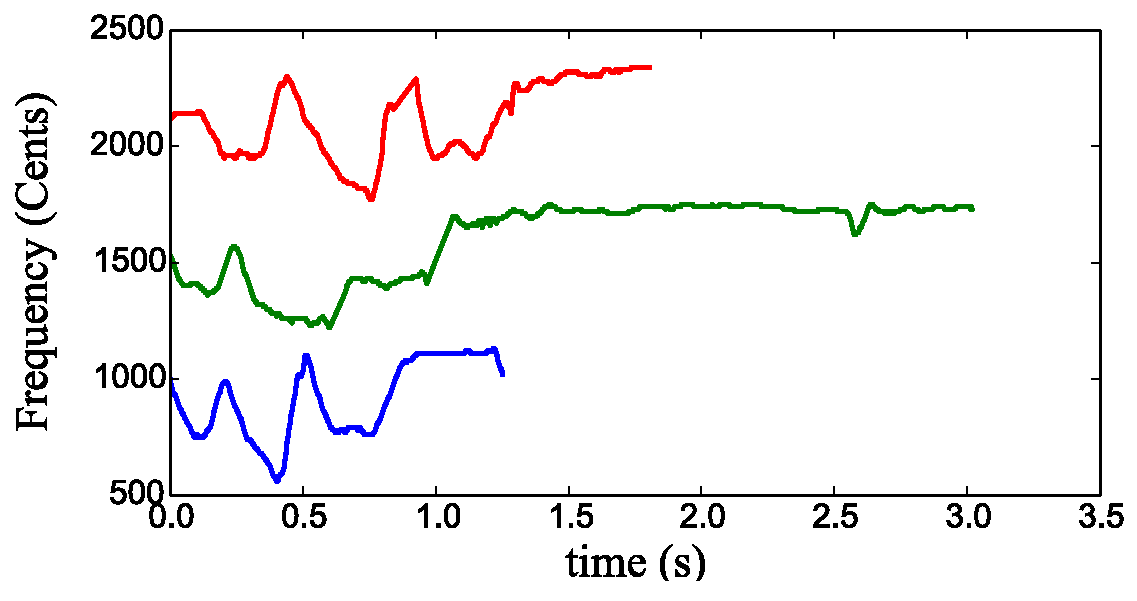
\includegraphics[width=\figSizeSixty]{ch06_patterns/figures/SimilarityEvaluation/Hindustani3Patts.pdf}
	\end{center}
	\caption[Example of difference occurrences of a melodic pattern]{Melodic fragments corresponding to three different renditions of the same characteristic \gls{raga} pattern in Hindustani music. For a better visualization, the patterns are transposed by a frequency offset of 600\,cents between them.}
	\label{fig:examples_3_phrases}
\end{figure}

Melodic similarity computation is a critical processing block within pattern processing in melodic sequences. In~\secref{sec:sota_pattern_processing_iam} and~\secref{sec:query_by_humming}, we review the existing approaches for melodic pattern processing, which directly or indirectly address the task of melodic similarity. From our review we see that the computational methods to assess melodic similarity have received considerable attention from the \gls{mir} community for a long time. A large number of studies focusing on melodic similarity work with a symbolic representation of music (\secref{sec:motif_in_symbolic_music}). When working with audio music signals, this topic has been studied in depth within the tasks of \acrfull{qbh} and pattern detection in audio recordings (see \secref{sec:query_by_humming} and \secref{sec:sota_pattern_processing_iam}).

The approaches proposed for computing melodic similarity primarily differ in the choices made for the main processing steps comprising; melody representation, melody segmentation, pitch transposition invariance, tempo or timing invariance, and distance measure (\secref{sec:query_by_humming}). In addition, every method has a  set of additional choices for selecting the optimal parameters at each processing step. Since the melodic characteristics across music traditions vary considerably, these procedures and parameter choices cannot be generalized to all music traditions. Therefore, studies that perform a comparative evaluation of different methods and analyze the effect of different parameter settings for a specific type of music material are valuable to the community~\citep{RBDannenberg2007QBH,Rao2014,XavierSerra2011}.

During the course of this thesis work several approaches have been proposed for computing melodic similarity in \gls{iam} (\secref{sec:sota_pattern_processing_iam}). However, a consensus on the best approach has yet not been reached. This is mainly because these approaches are evaluated using different datasets and under different experimental setup. To the best of our knowledge there has not been any study that systematically evaluates the influence of different choices of procedures and parameter values involved in similarity computation in melodies of \gls{iam}.



%In the literature (Section XX) there are a number of approaches proposed for computing melodic similarity\TODO{refs}. These approaches vary depending upon the melodic characteristics of a music tradition, duration of the melodic fragment and the task under study. There are a number of parameters and processing steps involved in the computation of melodic similarity such as the choice of melodic representation, frequency normalization and the distance measure. For music traditions such as XXX YYY kind of melodic representations are frequently used. some state of the art explanation.\TODO{This paragraph will be finished after literature review.}

%As seen in the literature review that a number of successful strategies for computing melodic similarity work on transcribed melodic representation\TODO{ref}. For \gls{iam}, where one of the characteristic aspects of melodies is its gliding transitory movement, transcription becomes a complex and an ill-defined task\TODO{ref}. Melodic representation directly influences the choice of an optimal distance measure. Therefore, due to all these factors there is need to comprehensively assess the influence of different system parameters and procedures on the accuracy of melodic similarity for \gls{iam}. 

%We study modeling of melodic similarity by casting it as a retrieval task. For this we use collections of audio recordings for which occurrences of characteristic melodic phrases of different \glspl{raga} are annotated by professional musicians~(\secref{sec:corpus_melodic_similarity_dataset}). We consider all the occurrences of a characteristic melodic phrase melodically more similar to each other than any random melodic fragment extracted from the collection. Thus, if we consider a characteristic melodic phrase as a query and compute melodic similarity with every possible melodic fragment in the collection, we expect all other occurrences of this characteristic phrase to appear on the top of the search results. Note that working with characteristic melodic phrases of \glspl{raga} for developing melodic similarity models adds to the complexity of the task. This is because while our system computes melodic similarity by comparing two melodic fragments, musician's have annotated these phrases by segmenting and identifying them individually. Characteristic melodic phrases of \glspl{raga} are distinctly recognizable by musicians and therefore annotating them do not involve any comparison of two melodic fragments. 

% In this section we address this issue by performing an exhaustive evaluation of several methodologies and parameter settings for computing similarity between short-time melodic patterns in \gls{iam}.


In this section, we describe a string matching-based approach for computing similarity between two short-time melodic patterns in \gls{iam}. Our objective is to perform a comprehensive evaluation of different variants of this approach to study the influence of different system parameters and procedures on melodic similarity for \gls{iam}. We evaluate 560 variants put together by combining different choices of the sampling rate of the melody representation, pitch quantization levels, melody normalization techniques, uniform time-scaling and distance measures. We believe the findings of this study will pave the way for developing unsupervised melodic pattern discovery approaches as described in the subsequent sections, whose evaluation is a challenging and, many times, ill-defined task. The current section is based on our published work presented in~\cite{gulati_ICASSP2015}.

\subsection{Method}
\label{sec:method_similarity_evaluation}


\begin{figure}
	\begin{center}
		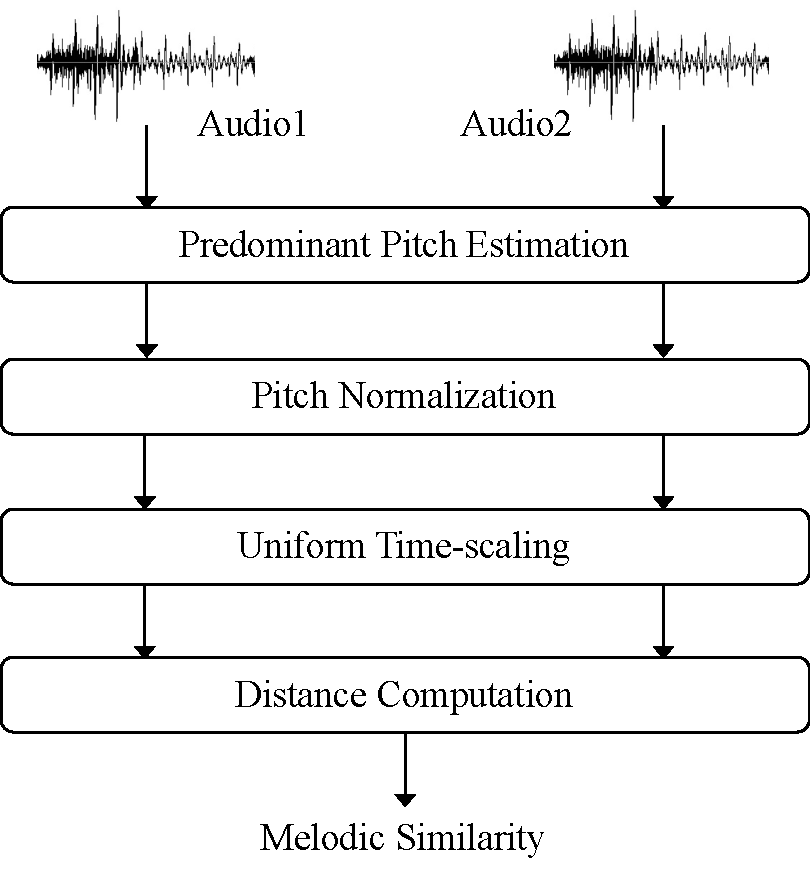
\includegraphics[width=\figSizeSixty]{ch06_patterns/figures/SimilarityEvaluation/melodic_similarity_blockd.pdf}
	\end{center}
	\caption[Block diagram for computing melodic similarity]{Block diagram of the methodology followed for computing melodic similarity from audio recordings.}
	\label{fig:block_diagram_melodic_similarity}
\end{figure}

The block diagram for computing melodic similarity is shown in~\figref{fig:block_diagram_melodic_similarity}. There are four main processing blocks involved in this task; predominant pitch estimation, pitch normalization, uniform time-scaling, and distance computation. We explore different combinations of the choices made for the processing steps and the parameter settings.

\subsubsection{Predominant Pitch Estimation}
\label{sec:patterns_melodic_similarity_representation}

We follow common practice and represent melody by the predominant pitch of an audio signal. For Carnatic music, we use a state-of-the-art melody extraction method proposed by~\cite{Salamon2012} as described in~\secref{sec:data_preprocessing_predominant_melody_estimation}. We use a frame size of 46\,ms and a hop size of 5\,ms. We do not perform any post-processing on the pitch contours except for interpolating short unvoiced segments (\secref{sec:data_processing_pitch_interpolation}). For Hindustani music we use semi-automatically extracted predominant pitch contours included in the dataset that we use to perform evaluations (\secref{sec:corpus_melodic_similarity_dataset}). This dataset along with these pitch contours have been used in several studies on similar topics~\citep{Rao2014,Ross2012b,Ross2012}. This eases the comparison of results across studies and also avoids the effect of pitch errors often present in fully automated melody extraction algorithms. We convert the pitch values from Hertz to Cents in order to make the representation musically more relevant (\secref{sec:data_processing_cent_conversion}).

Since automatic assessment of melodic similarity is a computationally expensive task, particularly when done on large audio archives, we desire the minimum possible sampling rate of the melody without compromising the accuracy. We therefore analyze the effect of different sampling rates of the melody representation on melodic similarity. We consider 5 sampling rates 100, 67, 50, 40 and 33\,Hz of predominant pitch, implemented by down-sampling the original melody sequence as described in~\secref{sec:data_processing_pitch_resampling}. We denote these parameter settings by $\sRate_{100}, \sRate_{67}, \sRate_{50}, \sRate_{40}$ and $\sRate_{33}$. Note that in our literature review we found that none of the existing approaches performed a systematic evaluation of this important parameter for melodies in \gls{iam}~(\secref{sec:sota_pattern_processing_iam}).

\subsubsection{Pitch Normalization}
\label{sec:patterns_melodic_similarity_transposition_invariance}

The absolute values of the pitch samples (in both Hertz and Cent scale) corresponding to different occurrences of a melodic pattern may differ across artists and even within the same recording. There are two main reasons for this. First, in \gls{iam} the reference frequency for a melody rendition is the tonic of the lead artist (\secref{sec:melody_in_iam}), which typically varies across artists. And second, a melodic pattern may recur in a different octave within the same recording. Therefore, a meaningful comparison of the melodic patterns across different artists and across different sections of a recording is possible only when the similarity computation is invariant to pitch transpositions. Out of these two cases, the latter is relatively infrequent, and is ignored in most of the existing studies (\secref{sec:sota_pattern_processing_iam}).

We experiment with five different normalization techniques to achieve pitch transposition invariance. They are as follows. 
\COMMENT{if time permits you can write an equation for each of them.}

\begin{enumerate}
	\item Normalizing the pitch values of a melodic pattern by the tonic of the lead artist of the recording ($\mNorm_{\mathrm{tonic}}$). This is implemented by considering the tonic frequency of the lead artist as the base frequency in Hertz to Cents conversion (see~\secref{sec:tonic_normalization})

	\item Zero mean normalization ($\mNorm_{\mathrm{mean}}$), where mean of the melodic pattern is subtracted from each pitch sample so that the resulting mean of the pattern becomes zero
	
	\item Zero median normalization ($\mNorm_{\mathrm{median}}$), where median of the melodic pattern is subtracted from each pitch sample so that the resulting median of the pattern becomes zero
	\item Z-normalization ($\mNorm_{\mathrm{Z}}$), where from each pitch sample we subtract the mean of the melodic pattern and subsequently divide it by the standard deviation of the pattern
	\item Median absolute deviation normalization ($\mNorm_{\mathrm{MAD}}$), where from each pitch sample we subtract the median of the melodic pattern and subsequently divide it by the median absolute deviation of the pattern
\end{enumerate}

In the case of $\mNorm_{\mathrm{tonic}}$ the tonic pitch of the lead artist is identified using \acrshort{tonicid_justin} method, the best performing method resulted from our exhaustive evaluations~(\secref{sec:pre_processing_tonic_identification_summary}). Furthermore, since the reference frequency of the melody is known for this case ($\mNorm_{\mathrm{tonic}}$), the pitch values can be quantized, as reported in other studies~\citep{Ross2012b}. Hence, we additionally experiment with two quantization levels; semitone level, quantizing pitch values to 100\,Cents interval ($\mNorm_{\mathrm{tonicQ12}}$) and quarter-tone level,  quantizing pitch values to 50\,Cents interval ($\mNorm_{\mathrm{tonicQ24}}$). Note that the tonic normalization ($\mNorm_{\mathrm{tonic}}$) is helpful only in the scenarios where the frequency transpositions are due to the different tonic frequencies of the lead artists across recordings. It does not handle the cases where a pattern recurs in a different octave or a tetra-chord within the same recording. In total, we consider 8 different normalization variants, including the one without any normalization ($\mNorm_{\mathrm{off}}$). 


\subsubsection{Uniform Time-scaling}
\label{sec:patterns_melodic_similarity_time_scaling}

In order to compensate for global tempo variations across occurrences of a melodic pattern, a typical approach is to consider multiple uniformly time-scaled versions of the patterns~\citep{mazzoni2001melody,zhu2003query,kotsifakos2012survey}. Such tempo differences if not handled can significantly degrade the performance in retrieval scenarios where fixed duration patterns are considered. We experiment with two possibilities; first,  we do not apply any time-scaling to the patterns ($\uTScaling_{\mathrm{off}}$) and second, we generate 5 copies of every pattern before similarity computation by uniformly time-scaling it by a factor of 0.9, 0.95, 1, 1.05 and 1.1 ($\uTScaling_{\mathrm{on}}$). We implement uniform time-scaling using cubic interpolation. 


\subsubsection{Distance Computation}
\label{sec:patterns_melodic_similarity_dissimilarity measures}

To measure the melodic similarity between two patterns we consider two categories of commonly used distance measures (see \secref{sec:sota_pattern_processing_iam} and \secref{sec:query_by_humming}); Euclidean distance ($\distPattMeasure_{\mathrm{Euc}}$) and \acrfull{dtw}-based distance. Euclidean distance is a non-parametric distance measure (\secref{sec:euclidean_distance}, \eqnref{eq:euclidean_distance}), whereas, \gls{dtw}-based distance measure has many variants and parameters to select. 

In this study we consider the whole sequence matching \gls{dtw} variant and two possibilities of the local constraint~(\secref{sec_DTW_distance_measure}):

\begin{itemize}
	\item  Where the \gls{dtw} step condition is $\lbrace(1,1), (1,1), (1,1)\rbrace$, which is without any local constraint. We denote this variant by~$\distPattMeasure_{\mathrm{DTW\_L0}}$. In this variant the \gls{dtw} accumulated cost matrix is computed using~\eqnref{eq:dtw_classic_cost_matrix_computation}.
	\item Where the \gls{dtw} step condition is $\lbrace(2,1), (1,1), (1,2)\rbrace$, which is with a local constraint We denote this variant by~$\distPattMeasure_{\mathrm{DTW\_L1}}$. In this variant the \gls{dtw} accumulated cost matrix is computed using~\eqnref{eq:dtw_local_constraint_cost_matrix_computation}.
\end{itemize}

In addition, for both these \gls{dtw} variants we also apply Sakoe-Chiba global band constraint~\citep{Sakoe78TASLP} with the width of the band as 5\%, 10\% and 90\% of the pattern length. Note that 90\% band width in the global constraint is to simulate the case of unconstrained \gls{dtw}. We denote these combinations by $\distPattMeasure_{\mathrm{DTW\_L0\_G5}}$, $\distPattMeasure_{\mathrm{DTW\_L0\_G10}}$, $\distPattMeasure_{\mathrm{DTW\_L0\_G90}}$, $\distPattMeasure_{\mathrm{DTW\_L1\_G5}}$, $\distPattMeasure_{\mathrm{DTW\_L1\_G10}}$, and $\distPattMeasure_{\mathrm{DTW\_L1\_G90}}$, respectively. In total, we consider 7 variants of distance measures for melodic similarity computation.

%
%In this study we consider the whole sequence matching \gls{dtw} variant and two possibilities of the local constraints; first, without any local constraint ($\distPattMeasure_{\mathrm{DTW\_L0}}$), where the \gls{dtw} step condition is $\lbrace(1,1), (1,1), (1,1)\rbrace$, and second, with local constraint ($\distPattMeasure_{\mathrm{DTW\_L1}}$), where $\lbrace(2,1), (1,1), (1,2)\rbrace$ is the \gls{dtw} step condition (see \secref{sec_DTW_distance_measure}). In addition, for both these \gls{dtw} variants we also apply Sakoe-Chiba global band constraint~\cite{Sakoe78TASLP} with the width of the band as 5\%, 10\% and 90\% of the pattern length. Note that 90\% band width in the global constraint is to simulate the case of unconstrained \gls{dtw}. We denote these combinations by $\distPattMeasure_{\mathrm{DTW\_L0\_G5}}$, $\distPattMeasure_{\mathrm{DTW\_L0\_G10}}$, $\distPattMeasure_{\mathrm{DTW\_L0\_G90}}$, $\distPattMeasure_{\mathrm{DTW\_L1\_G5}}$, $\distPattMeasure_{\mathrm{DTW\_L1\_G10}}$, and $\distPattMeasure_{\mathrm{DTW\_L1\_G90}}$, respectively. In total, we consider 7 variants of distance measures for melodic similarity computation.

Since the length of the melodic patterns are different, before computing similarity between two patterns we apply  a uniform time-scaling to make their lengths equal. We select the maximum of the lengths of the two patterns as the final length. This operation is a must for the Euclidean distance and has been shown to have a slightly beneficial effect for \gls{dtw}~\citep{Ratanamahatana2004,zhu2003query}.


\subsection{Evaluation Methodology}
\label{sec:patterns_melodic_similarity_evaluation_methodology}

We use \acrshort{msds} dataset for evaluating different variants of the method for computing melodic similarity (\secref{sec:corpus_melodic_similarity_dataset}). Since melodic characteristics across Carnatic and Hindustani music differ considerably, \acrshort{msds} comprises two sub-datasets, \acrshort{msds_iitm_cmd} and \acrshort{msds_iitb_hmd}. For evaluation of melodic similarity in Carnatic music we use \acrshort{msds_iitm_cmd} dataset, and in Hindustani music we use \acrshort{msds_iitb_hmd} dataset. Both these datasets contain annotations comprising occurrences of five different characteristic phrases of the \glspl{raga}~(\tabref{tab:categorywise_details_melodic_similarity_dataset}). Note that we regard each characteristic phrase as one type of a pattern.

We consider every annotated pattern as a query and perform an exhaustive search in the target search space comprising all the annotated patterns in the entire music collection. To make the experimental setup closer to the real world scenario, we add melodic segments other than the annotated patterns in the target search space, which act as noise (referred to as noise candidates). We generate these candidates by randomly selecting short fragments of the melodies from the dataset. The time stamps of the starting of these noise candidates are generated using a uniform distribution, and the lengths are determined using the distribution of the duration values of the annotated patterns. The total number of noise candidates added is 100 times the number of annotated patterns for each dataset. For every query, we order the search results by the similarity values and consider the top 1000 nearest neighbors for evaluation. A retrieved pattern is considered as a true hit only if it belongs to the same pattern type as the query pattern. 

In the experimental setup described above, the segmentation of the melodic patterns is done using the ground-truth annotations. However, in several tasks such as in melodic pattern discovery the segmentation information might not be present. Thus, to simulate a retrieval scenario where the pattern boundaries are not known \textit{a priori}, we also consider a simple extension to the experiment by assuming the target pattern length to be equal to the length of the query pattern. We perform all our experiments for both these setups. 

We evaluate all possible combinations of the choices made at each step of the melodic similarity computation discussed in~\secref{sec:method_similarity_evaluation}. We consider 5 different sampling rates of the melody representation, 8 different normalization scenarios, 2 possibilities of uniform time-scaling and 7 variants of the distance measures. In total, we evaluate 560 different variants.

To quantify the performance of a melodic similarity variant considered in this study we use \acrfull{map}, a typical evaluation measure in information retrieval~\citep{manning2008introduction}. \Gls{map} is computed by taking the mean of the average precision values of each query in the dataset. This way, we have a single number to evaluate and compare the performance of a variant. In order to assess if the difference in the performance of any two variants is statistically significant, we use the Wilcoxon signed rank-test~\citep{wilcoxon1945individual} with $\pVal < 0.01$. To compensate for multiple comparisons, we apply the Holm-Bonferroni method~\citep{holm1979simple}. Thus, considering that we compare 560 different variants, we effectively use a much more stringent criteria than $\pVal < 0.01$ for measuring statistical significance.


\subsection{Results and Discussion}
\label{sec:patterns_melodic_similarity_results_discussions}


\begin{table} 
	\begin{centering}
	\tabcolsep = 0.12cm
	\begin{tabular}{ c | c c c c c}
\tabletop
		Dataset   	& 	\acrshort{map}	&	Srate		&	Norm 	&	TScale 		&	Dist \\	
\tablemid
		\multirow{3}{*}{\acrshort{msds_iitm_cmd}}   	
		& 	0.413 	&	$\sRate_{67}$			&	$\mNorm_{\mathrm{mean}}$ 	&	$\uTScaling_{\mathrm{off}}$		&	$\distPattMeasure_{\mathrm{DTW\_L1\_G90}}$\\	
		& 	0.412 	&	$\sRate_{67}$		&	$\mNorm_{\mathrm{mean}}$ 	&	$\uTScaling_{\mathrm{on}}$		&	$\distPattMeasure_{\mathrm{DTW\_L1\_G10}}$\\	
		& 	0.411	&	$\sRate_{100}$		&	$\mNorm_{\mathrm{mean}}$ 	&	$\uTScaling_{\mathrm{off}}$		&	$\distPattMeasure_{\mathrm{DTW\_L1\_G90}}$\\	
		\hline		
		\multirow{3}{*}{\acrshort{msds_iitb_hmd}}   	
		& 	0.552	&	$\sRate_{100}$		&	$\mNorm_{\mathrm{tonic}}$ 	&	$\uTScaling_{\mathrm{off}}$		&	$\distPattMeasure_{\mathrm{DTW\_L0\_G90}}$\\	
		& 	0.551 	&	$\sRate_{67}$	&	$\mNorm_{\mathrm{tonic}}$ 	&	$\uTScaling_{\mathrm{off}}$		&	$\distPattMeasure_{\mathrm{DTW\_L0\_G90}}$\\	
		& 	0.547 	&	$\sRate_{50}$		&	$\mNorm_{\mathrm{tonic}}$ 	&	$\uTScaling_{\mathrm{off}}$		&	$\distPattMeasure_{\mathrm{DTW\_L0\_G90}}$\\	
\tablebot		
	\end{tabular}
	\caption[\acrshort{map} score and parameter details for the three best performing variants of the method for computing melodic similarity]{\acrshort{map} score and the details of parameter settings for the three best performing variants for \acrshort{msds_iitm_cmd} and \acrshort{msds_iitb_hmd}. Srate: sampling rate of the melody representation, Norm: normalization technique, TScale: uniform time-scaling and  Dist: distance measure.}
	\label{tab:melodic_similarity_results}
\par \end{centering}	
\end{table}


In this section we present the results of our evaluation of the 560 variants for each of the datasets, \acrshort{msds_iitm_cmd} and \acrshort{msds_iitb_hmd}. We order the variants in the decreasing order of their \gls{map} scores and present only the three best performing variants in~\tabref{tab:melodic_similarity_results}. For complete results see \url{http://compmusic.upf.edu/node/242}. \TODO{place better this link}

In Table~\ref{tab:melodic_similarity_results} (top half), we show the \gls{map} scores and the details of parameter settings for \acrshort{msds_iitm_cmd} dataset. We see that the best performing variant has a \gls{map} score of 0.413. Having a look at the whole list, we observe that for \acrshort{msds_iitm_cmd}, in the ranked list of the 560 variants, top performing variants consistently use higher sampling rates (either  $\sRate_{100}$, or $\sRate_{67}$). This can be attributed to the rapid oscillatory melodic movements present in Carnatic music, whose preservation requires a higher sampling rate. The top variants invariably use the zero mean normalization ($\mNorm_{\mathrm{mean}}$), suggesting that there are several repeated instances of the melodic patterns that are pitch transposed within the same recording. In addition, top variants also use \gls{dtw}-based distance with local constraint (either $\distPattMeasure_{\mathrm{DTW\_L1\_G10}}$ or $\distPattMeasure_{\mathrm{DTW\_L1\_G90}}$), indicating that melodic fragments are prone to large pathological warpings that can significantly degrade the performance. We do not observe any consistency in the usage of uniform time-scaling. However, it strongly correlates with the global constraint in the \gls{dtw} distance. In majority of the top ranked variants, $\uTScaling_{\mathrm{on}}$ consistently occurs with $\distPattMeasure_{\mathrm{DTW\_L1\_G10}}$, and $\uTScaling_{\mathrm{off}}$ consistently occurs with $\distPattMeasure_{\mathrm{DTW\_L1\_G90}}$. This suggests that a combination of uniform time-scaling and narrow global band constrained variant of \gls{dtw} is able to handle the same degree of non-linear timing variations as can be handled by a globally unconstrained \gls{dtw}. However, the former configuration is computationally more efficient than the latter. We also performed an analysis of several (small distance) false positives and found that the \gls{map} scores for a number of queries were low because of the spurious errors in the predominant pitch.


\begin{figure}
	\begin{center}
		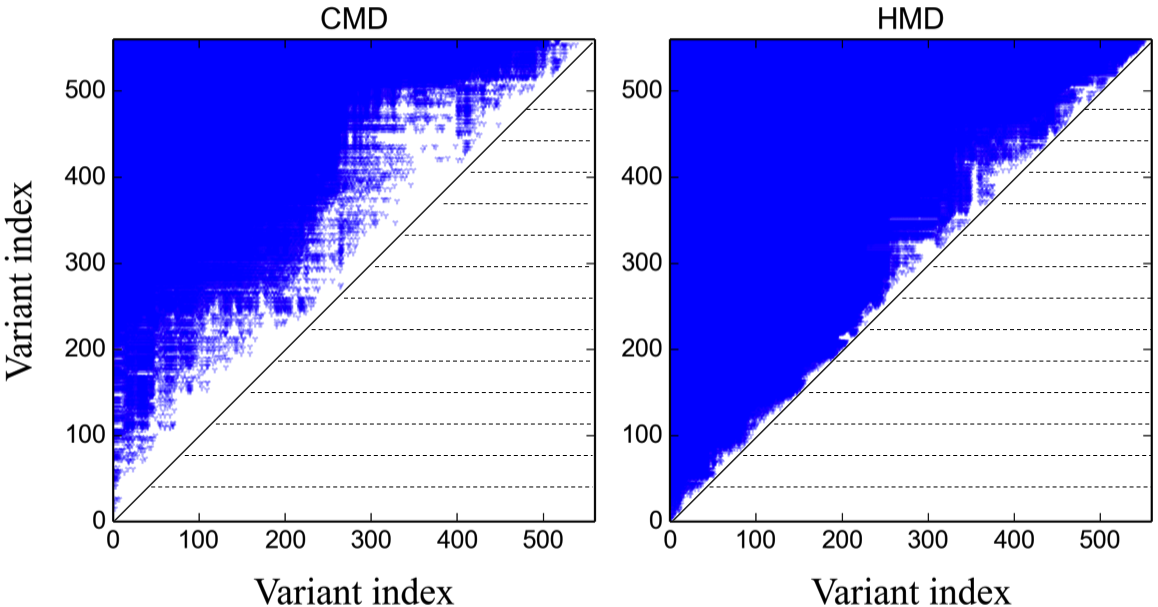
\includegraphics[width=\figSizeEightyFive]{ch06_patterns/figures/SimilarityEvaluation/StatisticalDiff.png}
	\end{center}
	\caption[Matrix indicating the statistical significance of the performance difference between different method variants]{Matrix indicating the statistical significance of the performance difference between every variant pair for \acrshort{msds_iitm_cmd} and \acrshort{msds_iitb_hmd}. Variant pairs where the difference in the performance is statistically significant are marked by dots. Only the superscript in the name of the dataset is used in the labels.\TODO{This figure uses symbol, check if it matches the text}}
	\label{fig:patterns_statistical_significance_similarity_evaluation}
\end{figure}


The \gls{map} scores and the details of parameter settings for \acrshort{msds_iitb_hmd} dataset are shown in~\tabref{tab:melodic_similarity_results} (bottom half). Compared to \acrshort{msds_iitm_cmd}, the best \gls{map} score for \acrshort{msds_iitb_hmd} is higher (0.55). Amongst the top ranked variants there is no consensus on the sampling rate of the melody representation. All the top ranked variants have the same parameter values except the sampling rate. This suggests that the sampling rates considered in this study have no significant effect on the melodic similarity for \acrshort{msds_iitb_hmd}. This can be attributed to the fact that the recordings in \acrshort{msds_iitb_hmd} are slow-medium tempo music pieces that do not have fast oscillatory melodic movements, as was the case with \acrshort{msds_iitm_cmd}.  Furthermore, for \acrshort{msds_iitb_hmd}, we observe that the variants using $\mNorm_{\mathrm{tonic}}$, $\mNorm_{\mathrm{tonicQ12}}$ or $\mNorm_{\mathrm{tonicQ24}}$ perform better than the ones using $\mNorm_{\mathrm{mean}}$, which is in contrast to the observation for \acrshort{msds_iitm_cmd}. This is primarily because in Carnatic music in our datasets there are many cases where a pattern recurs in a different octave within the same recording, whereas, in Hindustani music, such cases are rare. In general, we see that the \gls{dtw}-based distance performs better than the euclidean distance, and the \gls{dtw} variant without a global constraint ($\distPattMeasure_{\mathrm{DTW\_L1\_G90}}$ or $\distPattMeasure_{\mathrm{DTW\_L0\_G90}}$) is preferred. This implies that the repeated instances of melodic patterns in IAM (specifically in Hindustani music) have large non linear timing variations.

To assess the statistical significance of the results we compare every possible pair of the variants ($^{560}C_{2}$ = 156520 comparisons). The results are shown in~\figref{fig:patterns_statistical_significance_similarity_evaluation}, where both the axes are the index of the variants in the ranked list. For every variant pair with index $i$ and $j$, we mark the pixel~($i$,$j$) if the difference is statistically significant. From~\figref{fig:patterns_statistical_significance_similarity_evaluation} we see that a majority of variant pairs have a statistically significant difference in the \gls{map} scores. This indicates that the task of computing melodic similarity is sensitive to the choice of parameters and processing steps, and a small change in the choices made in a variant can lead to a significantly different \gls{map} score. Furthermore, as the marked pixels are higher in number for \acrshort{msds_iitb_hmd}, this sensitivity is even higher for \acrshort{msds_iitb_hmd} compared to \acrshort{msds_iitm_cmd}.


\begin{figure}
	\begin{center}
		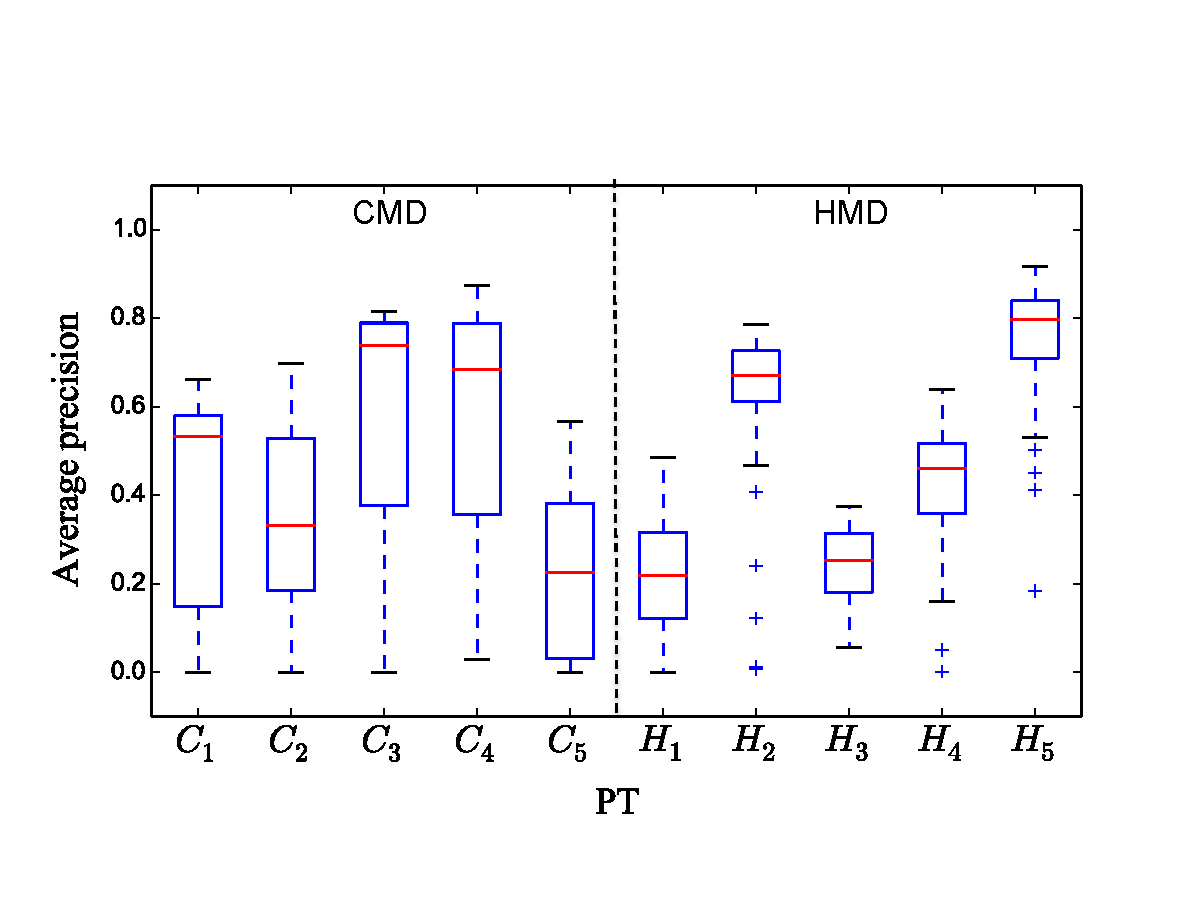
\includegraphics[width=\figSizeEightyFive]{ch06_patterns/figures/SimilarityEvaluation/CMD_HMD_CW_MAP.pdf}
	\end{center}
	\caption[Boxplot of average precision values for different types of melodic patterns]{Boxplot of the average precision values for each pattern type~(PT) in \acrshort{msds_iitm_cmd} and \acrshort{msds_iitb_hmd}. Only the superscript in the name of the dataset is used in the labels.\TODO{This figure uses symbol, check if it matches the text}}
	\label{fig:patterns_similarity_evaluation_results_boxplot}
\end{figure}


To analyze the consistency in the performance across pattern types, we present the boxplot of the average precision values for each pattern type in~\figref{fig:patterns_similarity_evaluation_results_boxplot}. For this, we consider only the top performing variant for each dataset. We see that the \gls{map} scores vary considerably across pattern types for both \acrshort{msds_iitm_cmd} and \acrshort{msds_iitb_hmd}. Furthermore, we observe that the intra pattern type variance of the \gls{map} scores is higher for \acrshort{msds_iitm_cmd} as compared to \acrshort{msds_iitb_hmd}. In addition, we observe that the pattern types $H_2$ and $H_5$ have a higher \gls{map} value compared to other pattern types in \acrshort{msds_iitb_hmd}. Interestingly, $H_2$ and $H_5$ are also the pattern types for which variance in the length is lower and number of occurrences is higher than others in \acrshort{msds_iitb_hmd} (\tabref{tab:categorywise_details_melodic_similarity_dataset}). This correlation is not evident in \acrshort{msds_iitm_cmd}. \COMMENT{there has to be a musical explanation here, whats happening? Ask Kaustuv and Vignesh}


\begin{table} 
	\begin{centering}
		\tabcolsep = 0.12cm
		\begin{tabular}{ c | c c c c c}
			\tabletop
			Dataset   	& 	\acrshort{map}	&	Srate		&	Norm 	&	TScale 		&	Dist \\	
			\tablemid
			\multirow{3}{*}{\acrshort{msds_iitm_cmd}}   	
			& 	0.279 	&	$\sRate_{67}$		&	$\mNorm_{\mathrm{mean}}$ 	&	$\uTScaling_{\mathrm{on}}$		&	$\distPattMeasure_{\mathrm{DTW\_L1\_G10}}$\\	
			& 	0.277 	&	$\sRate_{67}$		&	$\mNorm_{\mathrm{tonicQ12}}$ 	&	$\uTScaling_{\mathrm{on}}$		&	$\distPattMeasure_{\mathrm{DTW\_L1\_G10}}$\\	
			& 	0.275	&	$\sRate_{100}$		&	$\mNorm_{\mathrm{tonicQ12}}$ 	&	$\uTScaling_{\mathrm{on}}$		&	$\distPattMeasure_{\mathrm{DTW\_L1\_G10}}$\\	
\tablemid
			\multirow{3}{*}{\acrshort{msds_iitb_hmd}}   	
			& 	0.259	&	$\sRate_{40}$		&	$\mNorm_{\mathrm{tonicQ12}}$ 	&	$\uTScaling_{\mathrm{on}}$		&	$\distPattMeasure_{\mathrm{DTW\_L1\_G90}}$\\	
			& 	0.259 	&	$\sRate_{100}$		&	$\mNorm_{\mathrm{tonicQ12}}$ 	&	$\uTScaling_{\mathrm{on}}$		&	$\distPattMeasure_{\mathrm{DTW\_L1\_G90}}$\\	
			& 	0.259 	&	$\sRate_{67}$		&	$\mNorm_{\mathrm{tonicQ12}}$ 	&	$\uTScaling_{\mathrm{on}}$		&	$\distPattMeasure_{\mathrm{DTW\_L1\_G90}}$\\	
			\tablebot		
		\end{tabular}
		\caption[\acrshort{map} score and parameter details for the three best performing variants of the method for computing melodic similarity, without using groundth-truth segmentation]{\acrshort{map} score and the details of parameter settings for the three best performing variants for \acrshort{msds_iitm_cmd} and \acrshort{msds_iitb_hmd} dataset. These results are corresponding to the experiment where target patterns' length is not read from the ground-truth annotations but is considered to be same as the query pattern length. Srate: sampling rate of the melody representation, Norm: normalization technique, TScale: uniform time-scaling and  Dist: distance measure.}
		\label{tab:melodic_similarity_results_var2}
\par \end{centering}		
\end{table}

So far we have seen the results in the experimental setup where the melodic patterns are segmented using the ground-truth annotations. We now present the results corresponding to the other experimental setup described in~\secref{sec:patterns_melodic_similarity_evaluation_methodology}, where the target pattern lengths are considered to be the same as that of the query pattern. We evaluate all 560 variants of the method as done above on both the datasets under this experimental setup. In~\tabref{tab:melodic_similarity_results_var2} we show the \gls{map} scores of the top performing variants for both the datasets \acrshort{msds_iitm_cmd} and \acrshort{msds_iitb_hmd}. We find that the \gls{map} score for the best performing variant decreases from 0.41 to 0.28 and 0.55 to 0.26 for \acrshort{msds_iitm_cmd} and \acrshort{msds_iitb_hmd}, respectively. This indicates that the melodic similarity computation task becomes much more challenging in the absence of an accurate melodic segmentation method. For this experimental setup the trend in the sampling rate for Carnatic and Hindustani music remain the same as we saw in~\tabref{tab:melodic_similarity_results}, which is that a higher sampling rate is desired for representing melodic patterns in Carnatic music. In terms of the normalization we see that surprisingly $\mNorm_{\mathrm{tonicQ12}}$ is used by the top performing variants for both the datasets. Note that in other variants whose performance is not statistically significantly different from the ones reported in~\tabref{tab:melodic_similarity_results_var2}, $\mNorm_{\mathrm{mean}}$ and $\mNorm_{\mathrm{tonic}}$ normalization is also used for \acrshort{msds_iitm_cmd} and \acrshort{msds_iitm_cmd} dataset respectively. An interesting observation is that in this experimental setup uniform time-scaling is consistently used by all the top performing variants. This indicates that such a time-scaling operation is immensely advantageous in the retrieval scenarios where the length of the target melodic patterns is taken to be the same as that of a query pattern (i.e.~pattern segmentation is not known). We also see that $\distPattMeasure_{\mathrm{DTW\_L1\_G10}}$ and $\distPattMeasure_{\mathrm{DTW\_L1\_G90}}$ are always used for \acrshort{msds_iitm_cmd} and \acrshort{msds_iitb_hmd} datasets, respectively, indicting that applying a local constraint in \gls{dtw} is critical for this experimental setup.

\TODO{This is an important comment}
\COMMENT{If time permits it would be awesome to show accuracy as a function of different choices of parameters keeping others at an optimal value for both the traditions. That would make things very clear and impressive. Please do this!!!}


%################################################################################################################
%########################################### IMPROVING MELODIC SIMILARITY #######################################
%################################################################################################################

\section{Improving Melodic Similarity}
\label{sec:patterns_improving_melodic_similarity}

In the previous section we performed an exhaustive comparison of different procedures and parameter settings typically involved in the computation of melodic similarity (\secref{sec:patterns_evaluation_of_similarity_measures}). We learned about the impact of the different methodologies on the accuracy of the system, and about the best set of parameter settings for computing melodic similarity in \gls{iam}. Results indicate that this task is challenging, and even in the case of the best methodology, there exists a large scope for improvement. In this section we build upon our findings in \secref{sec:patterns_evaluation_of_similarity_measures} and investigate the exploitation of specific melodic characteristics of Hindustani and Carnatic music to further improve melodic similarity. 

From our literature review presented in \secref{sec:background_relevant_work_other_music} and \secref{sec:background_relevant_work_iam} we see that the methodologies for computing melodic similarity varies depending on the type of music material (sheet music or audio, monophonic or polyphonic)~\citep{Marsden2012,meredith2002algorithms,Cambouropoulos2001,collins2014bridging,ghias1995query,dannenberg2007comparative,mazzoni2001melody} and the music tradition~\citep{Juhasz2009a, Conklin2010a,Lartillot2006,pikrakis2003recognition}. Existing literature also indicates that the important characteristics of several melody-dominant music traditions of the world such as Flamenco and \gls{iam} need dedicated research efforts to devise approaches for computing melodic similarity~\citep{gomez2012automatic,pikrakis2012tracking,pikrakis2016detection,Rao2014}. With this spirit of devising culture specific approaches several methods for retrieving different types of melodic patterns have been proposed for \gls{iam} during the course of this dissertation~\citep{Ross2012b,Ross2012,ishwar2012motivic,Rao2014,Ishwar2013,Dutta2014,dutta2014modified}. 

We recapitulate briefly the approaches reviewed in \secref{sec:background_relevant_work_iam} that exploit specificities in \gls{iam}.  \cite{Ishwar2013} propose a saddle point based representation of melody that exploits the presence of \glspl{gamaka} in Carnatic music. This representation is used in the first stage of a two-stage process to prune the target search space. \cite{dutta2014modified} propose to modify the intermediate steps involved in the computation of the \gls{rlcs} distance to make it more suitable to the melodic sequences in Carnatic music.  \cite{Ross2012b} utilize the \gls{sama} locations to reduce the search space for detecting the \gls{mukhda} patterns of a composition in Hindustani music. \cite{Ross2012} pruned the search space by employing a melodic landmark called \gls{nyas} \gls{svara}. \cite{Rao2014} address the challenge of a large within-class variability in the occurrences of the characteristic phrases of \glspl{raga}. They propose to use exemplar-based matching after vector quantization-based training to obtain multiple templates for a given phrase category. In addition, the authors also propose to learn an optimal \gls{dtw} constraint for each phrase category in order to exploit the possible patterns in the duration variability of melodic phrases in Hindustani music. 

The approaches mentioned above are directed towards developing culturally informed and knowledge-driven computational methodologies. However, as we notice, there is a large scope for further improvement in this area. One of the main shortcomings of nearly all these existing approaches is their scalability to different musical forms and styles within \gls{iam}. Most of these approaches are proposed and evaluated on either Hindustani or Carnatic music. Even within these two music traditions they focus on a certain type of melodic patterns, musical style, and in some cases, to only slow tempo (vilambit laya) music compositions. For example, \gls{sama} location can indicate roughly the onset of a \gls{mukhda} phrase in an recording of Hindustani music~\citep{Ross2012b}. But, it has no musically established relationship with the location of the characteristic melodic phrases of \glspl{raga}. Similarly, the Pa \gls{nyas} segmentation strategy followed in~\cite{Ross2012} can work only with the melodic phrases ending in the Pa \gls{svara}, and mainly for slow tempo compositions where the concept of \gls{nyas} \gls{svara} is evident. Thus, these approaches do not generalize and scale to other types of melodic patterns and to large music collections of \gls{iam}. Moreover, detecting these landmarks is a challenging task in itself~\citep{srinivasamurthy2014supervised,gulati2014Landmark}. Some of the above mentioned approaches also propose solutions to handle large within-class variability in melodic patterns, but they are suitable for a supervised analysis of melodic patterns and are clearly not applicable to unsupervised analysis. Our objective here is to devise an approach that can utilize specific melodic characteristics in \gls{iam}, and at the same time generalize to different musical forms and styles within this music tradition.

\begin{figure}
	\begin{center}
		\includegraphics[width=\figSizeHundred]{ch06_patterns/figures/ImprovingSimilarity/phraseClassesExample.pdf}
	\end{center}
	\caption[Examples of different occurrences of the \gls{raga} motifs]{Pitch contours of occurrences of three different characteristic melodic phrases in Hindustani music. Contours are frequency transposed and time shifted for a better visualization.}
	\label{fig:phraseComplexityExample}
\end{figure}

Before proceeding further it is worth revising the main challenges involved in the computation of melodic similarity for characteristic melodic phrases of \glspl{raga}. As already mentioned, the characteristic melodic phrases act as the basis for the artists to improvise, providing them with a medium to express creativity during a \gls{raga} rendition. Hence, the surface representation of these melodic phrases can vary a lot across their occurrences. This high degree of variability in terms of the duration of a phrase, non-linear time warpings and the added melodic ornaments together pose a big challenge for melodic similarity computation. In Figure~\ref{fig:phraseComplexityExample} we illustrate this variability by showing the pitch contours of the different occurrences of three characteristic melodic phrases of the \gls{raga} Alaiya Bilawal. We can clearly see that the duration of a phrase across its occurrences varies a lot and the steady melodic regions are highly varied in terms of the duration and the presence of melodic ornaments. Because of these factors detecting the occurrences of characteristic melodic phrases becomes a challenging task. Ideally, a melodic similarity measure should be robust to such high degree of melodic variations and, at the same time, it should be able to discriminate between different phrase categories and irrelevant melodic fragments (noise candidates).

In this section, we present two approaches that utilize specific melodic characteristics in \gls{iam} to improve melodic similarity. We describe a melodic abstraction process based on a partial transcription of melodies to handle large timing variations across occurrences of melodic phrases. Specifically for Carnatic music we also present a complexity weighting scheme that accounts for the differences in the melodic complexities of the phrases, a crucial aspect for melodic similarity in this music tradition. The following sections are based on our work presented in~\cite{gulati_ISMIR_2015}.

\COMMENT{Highlight that we are incorporating and exploiting universal or transversal kind of characteristics. Specific nuances which are often raga specific and are very important for melodic similarity might be not possible since we do not have comprehensive annotated dataset.}


\subsection{Method}
\label{sec:patterns_improving_similarity_method}

Before we present our approach in detail we first discuss the motivation and rationale behind it. A close examination of the occurrences of the characteristic melodic phrases in our dataset reveals that there is a pattern in the non-linear timing variations, which is also reported in~\cite{Rao2014}. In~\figref{fig:phraseComplexityExample} we show a few occurrences of three such melodic phrases. In particular, we see that the transient regions of a melodic phrase tend to span nearly the same time duration across different occurrences, whereas the stationary regions vary a lot in terms of the duration. In~\figref{fig:flatCompressionExample} we further illustrate this by showing two occurrences of a melodic phrase ($\pattern_{1a}$ and $\pattern_{2a}$). The stationary \gls{svara} regions are highlighted. We clearly see that the duration variation is prominent in the highlighted regions. To handle such large non-linear timing variations typically a non-constrained \gls{dtw} distance measure is employed~(\secref{sec:patterns_melodic_similarity_results_discussions}). However, such a \gls{dtw} variant is prone to noisy matches. Moreover, the absence of a band constraint renders it inefficient for computationally complex tasks such as pattern discovery~(\secref{sec:patterns_melodic_pattern_discovery}).

We put forward an approach that abstracts the melodic representation and reduces the extent of duration and pitch variations across the occurrences of a melodic phrase. Our approach is based on the partial transcription of the melodies.  As mentioned earlier, melodic transcription in \gls{iam} is a challenging task. The main challenges arise due to the presence of non-discrete pitch movements such as smooth glides and \glspl{gamaka}. However, since the duration variation exists mainly during the steady \gls{svara} regions, transcribing only the stable melodic regions might be sufficient. Once transcribed, we can then truncate the duration of these steady melodic regions and hence effectively reduce the amount of timing variations across the occurrences of a melodic phrase. Additionally, since the duration truncation also reduces the overall length of a pattern, the computational time for melodic similarity computation is also reduced substantially. Furthermore, this solution is independent of the distance measure used in the melodic similarity computation. Hence, it can be used even in the computationally complex tasks such as large scale pattern discovery, where the usage of distance lower bounds is imperative~(\secref{sec:patterns_melodic_pattern_discovery}).

\begin{figure}
	\begin{center}
		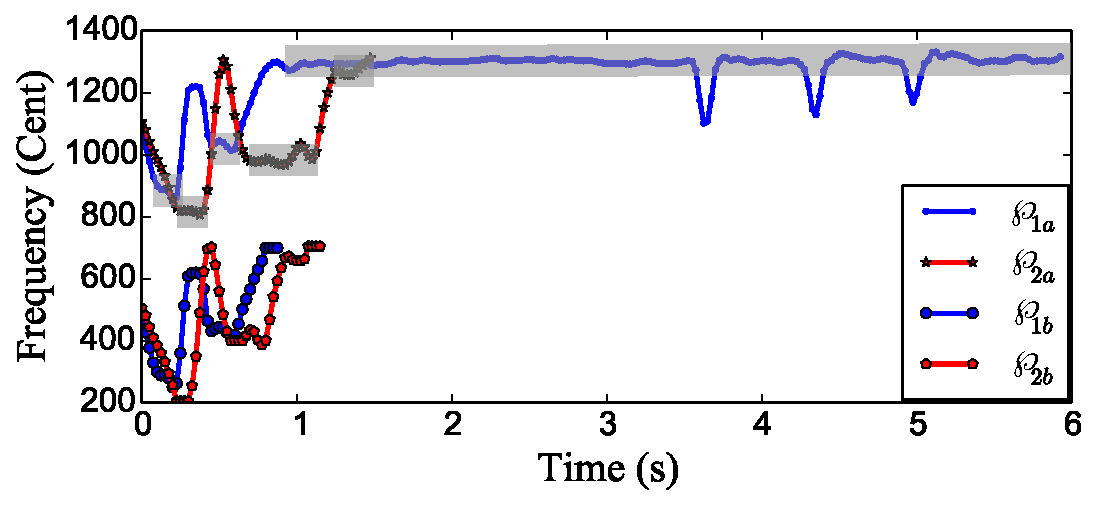
\includegraphics[width=\figSizeEightyFive]{ch06_patterns/figures/ImprovingSimilarity/Hindusani_flat_note_compression_example_reversed.pdf}
	\end{center}
	\caption[Example of melodic patterns after duration truncation]{Original pitch contours ($\pattern_{1a}$, $\pattern_{2a}$) and duration truncated pitch contours ($\pattern_{1b}$, $\pattern_{2b}$) of two occurrences of a characteristic phrase of \gls{raga} Alhaiya Bilawal. The contours are transposed for a good visualization.\TODO{This figure uses symbol, check if it matches the text}}
	\label{fig:flatCompressionExample}
\end{figure}

\begin{figure}
	\begin{center}
		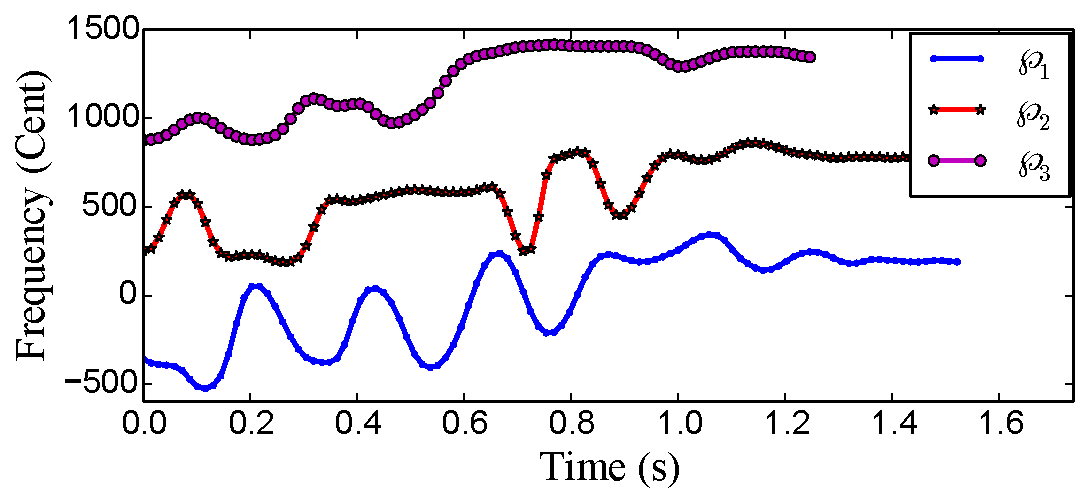
\includegraphics[width=\figSizeEightyFive]{ch06_patterns/figures/ImprovingSimilarity/CarnaticComplexityExample.pdf}
	\end{center}
	\caption[Illustration of an erroneous case of melodic similarity in Carnatic music]{Pitch contours of three melodic phrases ($\pattern_1$, $\pattern_2$, $\pattern_3$). $\pattern_1$ and $\pattern_2$ are the occurrences of the same characteristic phrase and both are musically dissimilar to $\pattern_3$.\TODO{This figure uses symbol, check if it matches the text}} 
	\label{fig:carnaticComplexityExample}
\end{figure}

The rapid oscillatory pitch movements (\glspl{gamaka}) in Carnatic music bring up another set of challenges for the melodic similarity computation. Very often, two musically dissimilar melodic phrases obtain a high similarity score owing to a similar pitch contour at a macro level. However, they differ significantly at a micro level. In~\figref{fig:carnaticComplexityExample} we illustrate such a case where we show the pitch contours of three melodic phrases $\pattern_1$, $\pattern_2$ and $\pattern_3$, where $\pattern_1$ and $\pattern_2$ are the occurrences of the same melodic phrase and both are musically dissimilar to $\pattern_3$. Using the best performing variant of the similarity measure obtained in~\secref{sec:patterns_melodic_similarity_results_discussions} (\tabref{tab:melodic_similarity_results}) we obtain a higher similarity score between the pairs ($\pattern_1$, $\pattern_3$) and ($\pattern_2$, $\pattern_3$) compared to the score between the pair ($\pattern_1$, $\pattern_2$). This tendency of a high complexity time-series (higher degree of micro level variations) obtaining a high similarity score with another low complexity time-series is discussed in~\cite{batista2011complexity}. We follow their approach and apply a complexity weighting to account for the differences in the melodic complexities between phrases in the computation of melodic similarity. 


We now proceed to describe our method in detail. The block diagram for computing melodic similarity is very similar to the one described in~\secref{sec:method_similarity_evaluation}. The main differences are the added processing blocks for performing partial transcription, \gls{svara} duration truncation and complexity weighting as shown in~\figref{fig:block_diagram_melodic_similarity_improved}. In the subsequent sections we describe every processing block in detail. 

\begin{figure}
	\begin{center}
		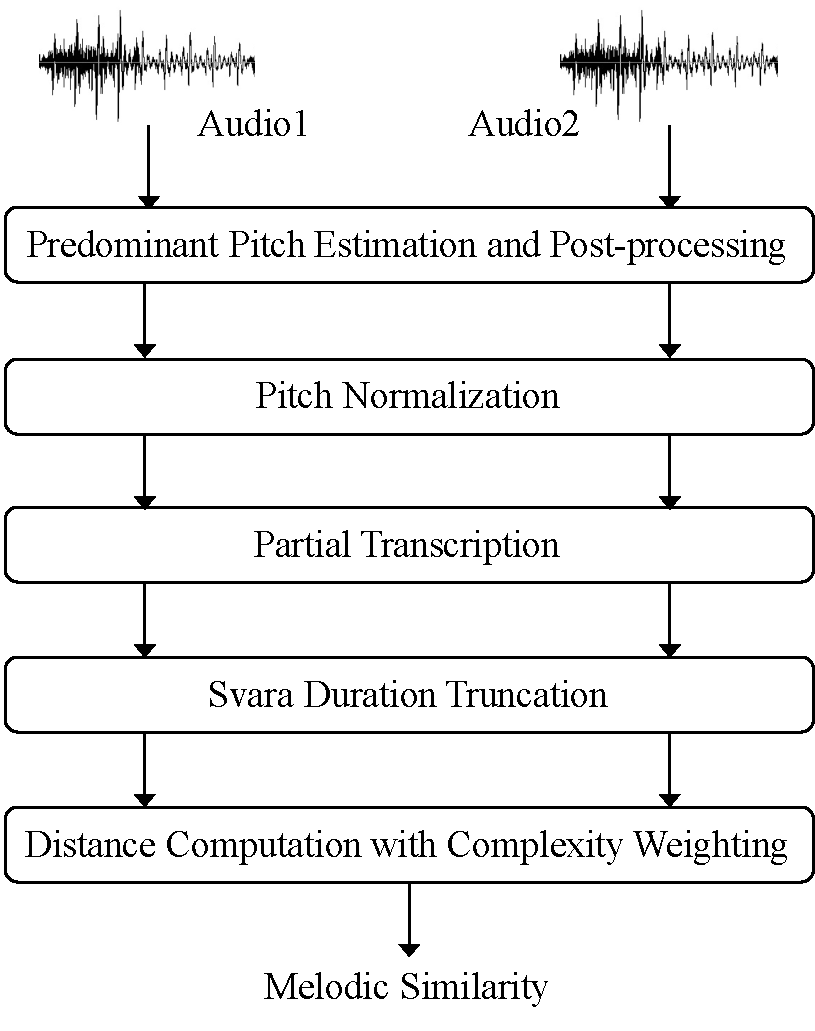
\includegraphics[width=\figSizeSixty]{ch06_patterns/figures/ImprovingSimilarity/melodic_similarity_improve_blockd.pdf}
	\end{center}
	\caption[Block diagram for an improved melodic similarity computation]{Block diagram of the improved methodology for computing melodic similarity} 
	\label{fig:block_diagram_melodic_similarity_improved}
\end{figure}

\subsubsection{Predominant Pitch Estimation and post-processing}
\label{sec:patterns_improving_similarity_melody_estimation}

As done before, we represent melody of an audio signal by the pitch of the predominant melodic source. For predominant pitch estimation we follow exactly the same procedure and use the same parameter values as done in~\secref{sec:patterns_melodic_similarity_representation}, which is explained in detail in~\secref{sec:data_preprocessing_predominant_melody_estimation}. After estimating the predominant pitch we convert it from Hertz to Cent scale for the melody representation to be musically relevant~(\secref{sec:data_processing_cent_conversion}).

We proceed to post-process the pitch contours to remove the spurious pitch jumps lasting over a few frames as well as to smooth the pitch contours. We follow the procedure described in~\secref{sec:data_processing_pitch_smoothening} and use exactly the same set of parameter values. The pitch contours are finally down-sampled to 67\,Hz (\secref{sec:data_processing_pitch_resampling}). This sampling rate was found to be working well for both Carnatic and Hindustani music in our earlier study that evaluated five different sampling rates~\secref{sec:patterns_melodic_similarity_results_discussions}.


\subsubsection{Pitch Normalization}
\label{sec:patterns_improving_similarity_transposition_invariance}

The base frequency chosen for a melody in \gls{iam} is the tonic pitch of the lead artist~(\secref{sec:data_preprocessing_tonic_identification}). Therefore, for a meaningful comparison of the melodic phrases across the recordings of different artists, a melody representation should be normalized by the tonic pitch of the lead artist. We perform this tonic normalization ($\mNorm_\mathrm{tonic}$) by considering the tonic of the lead artist as the reference frequency during the Hertz to Cent conversion as shown in~\secref{sec:data_processing_cent_conversion}. The tonic pitch is automatically identified using \acrshort{tonicid_justin} method, which performed the best in our comparative evaluation of seven different approaches~(\secref{sec:pre_processing_tonic_identification_results}).

Tonic normalization does not account for the pitch of the octave transposed occurrences of a melodic phrase within a recording. In addition, estimated tonic pitch sometimes might be incorrect and a typical error is an offset of an octave or a fifth scale degree in some cases. To handle such cases, we propose a tetrachord normalization ($\mNorm_\mathrm{tetra}$). For this we analyse the difference ($\pitchDiff_m$) in the mean frequency values of the two tonic normalized melodic phrases ($\pattern_1$, $\pattern_2$). We offset the pitch values of the phrase $\pattern_1$ by the frequency (Cents) in the set $\lbrace$-\,1200, -\,700, -\,500, 0, 500, 700, 1200, 1700, 1900$\rbrace$ that is closest to $\pitchDiff_m$ within a vicinity of 100\,Cents. In addition to tetrachord normalization, we also experiment with mean normalization ($\mNorm_\mathrm{mean}$), which was reported to improve the performance in the case of Carnatic music~(\secref{sec:patterns_melodic_similarity_results_discussions}). 


\subsubsection{Partial Transcription}
\label{sec:patterns_improving_similarity_partial_transcription}

We perform a partial melody transcription to automatically segment and identify the steady \gls{svara} regions in a melody. Note that even a partial transcription of the melodies is a non-trivial task, since we desire a segmentation that is robust to different melodic ornaments added to a \gls{svara} where the pitch deviation from the mean \gls{svara} frequency can be up to 200\,Cents. In~\figref{fig:flatCompressionExample} we show such an example of a steady \gls{svara} region ($\pattern_{1a}$ from 3-6\,s) where the pitch deviation from the mean \gls{svara} frequency is high due to added melodic ornaments. Ideally, the melodic region between 1 and 6\,s should be detected as a single \gls{svara} segment.

We segment the steady \gls{svara} regions using a method described in~\cite{gulati2014Landmark} (\secref{sec:pre_processing_nyas_segmentation}), which addresses the aforementioned challenges. A segmented \gls{svara} region is then assigned a frequency value corresponding to the peak in an aggregated pitch histogram closest to the mean \gls{svara} frequency. The pitch histogram is constructed for the entire recording and smoothened using a Gaussian window with a variance of 15\,Cents. As peaks of the normalized pitch histogram, we select all the local maximas where at least one peak-to-valley ratio is greater than 0.01. A detailed description of this method is provided in~\secref{sec:pre_processing_nyas_segmentation}.
 
\subsubsection{Svara Duration Truncation}
\label{sec:patterns_improving_similarity_svara_duration_trucation}

After segmenting the steady \gls{svara} regions in the melodies we proceed to truncate the duration of these regions. We hypothesize that, beyond a certain value $\svarTruncThsld$, the duration of these steady \gls{svara} regions do not change the identity of a melodic phrase (i.e.~the phrase category). We experiment with 7 different truncation durations $\svarTruncThsld = \lbrace$ 0.1\,s, 0.3\,s, 0.5\,s, 0.75\,s, 1\,s, 1.5\,s, 2\,s$\rbrace$ and select the one that results in the best performance. In~\figref{fig:flatCompressionExample}
we show an example of the occurrences of a melodic phrase both before ($\pattern_{1a}$, $\pattern_{2a}$) and after ($\pattern_{1b}$, $\pattern_{2b}$) the \gls{svara} duration truncation using $\svarTruncThsld = 0.1$\,s. This example clearly illustrates that the occurrences of a melodic phrase after duration truncation exhibit lower degree of non-linear timing variations. We denote this method by \acrshort{similarity_dt}.

\subsubsection{Distance Computation}
\label{sec:patterns_improving_similarity_similarity_computation}

To measure the similarity between two melodic fragments we consider a \gls{dtw}-based distance measure. Since the phrase segmentation is known beforehand, we use a whole sequence matching \gls{dtw} variant. We consider the best performing \gls{dtw} variant and the related parameter values for each music tradition as reported in~\secref{sec:patterns_melodic_similarity_results_discussions}. These variants were chosen based on an exhaustive grid search across all possible combinations and hence can be considered as optimal for this dataset. We use Sakoe-Chiba global band constraint~\cite{Sakoe78TASLP} with the width of the band as $\pm10$\% of the phrase length. Before computing the \gls{dtw} distance we uniformly time-scale the two melodic fragments to the same length, which is the maximum of the lengths of the phrases. Notice that even though in~\secref{sec:patterns_melodic_similarity_results_discussions} we found that a globally unconstrained \gls{dtw} variant ($\distPattMeasure_{\mathrm{DTW\_L0\_G90}}$) is an optimal choice for computing melodic similarity in Hindustani music, we restrict ourselves to a band-width of 10\% in this study. The main reason is because an unconstrained \gls{dtw} variant due to its computational complexity is not suitable for a large scale pattern discovery task~(\secref{sec:patterns_melodic_pattern_discovery}). Since one the main objectives of studying melodic similarity within a supervised setup in this work is to be finally able to apply the findings in an unsupervised analysis, we now restrict to choices that are also available and feasible in an unsupervised analysis.


\subsubsection{Complexity Weighting}
\label{sec:patterns_improving_similarity_complexity_invariance_weighting}

The complexity weighting that we apply here to overcome the shortcoming of the distance measure in distinguishing two time series with different complexities is discussed in~\cite{batista2011complexity}. We apply a complexity weighting ($\compWght$) to the \gls{dtw}-based distance ($\distPattMeasure_\mathrm{DTW}$) in order to compute the final similarity score $\distPattMeasure_{f}=\compWght \distPattMeasure_\mathrm{DTW}$. We compute $\compWght$ as:


\begin{equation}
\begin{gathered}
\compWght = \frac{\max(\compEst_i,\compEst_j)}{\min(\compEst_i, \compEst_j)} \\
%\compEst_i = \sqrt[2]{\sum_{i=1}^{N-1} (\pitchCents_{i}-\pitchCents_{i+1})^2}\\
\end{gathered}
\label{eq:complexity_weighing}
\end{equation}

\begin{equation}
\begin{gathered}
%\compWght = \frac{\max(\compEst_i,\compEst_j)}{\min(\compEst_i, \compEst_j)} \\
\compEst_i = \sqrt[2]{\sum_{i=1}^{N-1} (\pitchCents_{i}-\pitchCents_{i+1})^2}\\
\end{gathered}
\label{eq:complexity_estimate_batista}
\end{equation}

\noindent where, $\compEst_i$ is the complexity estimate of a melodic pattern of length $N$ samples and $\pitchCents_i$ is the pitch value of the $i^{\mathrm{th}}$ sample. We explore two variants of this complexity estimate. One of these variants is already proposed in~\cite{batista2011complexity} and is described in~\eqnref{eq:complexity_estimate_batista}. We denote this method variant by \acrshort{similarity_cw1}. We propose another variant that utilizes melodic characteristics of Carnatic music. This variant takes the number of saddle points in the melodic phrase as the complexity estimate~\citep{Ishwar2013}. This method variant is denoted by \acrshort{similarity_cw2}. As saddle points we consider all the local minimas and the local maximas in the pitch contour which have at least one minima to maxima distance of half a semitone. Since such melodic characteristics are predominantly present in Carnatic music, the complexity weighting is not applicable for computing melodic similarity in Hindustani music.


\subsection{Evaluation}
\label{sec:patterns_improving_similarity_evaluation}

\subsubsection{Dataset and Annotations}
\label{sec:patterns_improving_similarity_dataset_and_annotations}

For evaluation we use the same music collection as used in~\secref{sec:patterns_evaluation_of_similarity_measures}, which is described in~\secref{sec:corpus_melodic_similarity_dataset}. This collection enables a better comparison of the results with other studies since it has been used in several other studies for a similar task~\citep{Rao2014,Ross2012b}. However, we found a number of issues in the annotations of the melodic phrases, which we corrected and also extended the dataset by adding 25\% more number of melodic phrase annotations as explained in~\secref{sec:corpus_melodic_similarity_dataset}. We denote this new dataset by \acrshort{msds_cm} and the comprising Carnatic and Hindustani sub-datasets by \acrshort{msds_cm_cmd} and \acrshort{msds_cm_hmd}, respectively. Similar to the way we perform evaluations in~\secref{sec:patterns_evaluation_of_similarity_measures}, we evaluate our approach separately on both Carnatic and Hindustani datasets. In~\tabref{tab:melodic_similarity_dataset_details} we summarize the relevant details of the dataset in terms of the number of artists, \glspl{raga}, audio recordings and total duration. In~\tabref{tab:categorywise_details_revised_melodic_similarity_dataset} we summarize the details of the annotated phrases in terms of their number of instances and basic statistics of the length of the phrases.


\subsubsection{Setup, Measures and Statistical Significance}
\label{sec:patterns_improving_similarity_experimental_setup}

The experimental setup and evaluation measures used in this study are exactly the same as used for the comparative evaluation described in~\secref{sec:patterns_evaluation_of_similarity_measures}. We consider each annotated melodic phrase as a query and perform a search across all the annotated phrases in the dataset (referred to as target search space). In addition to the annotated phrases, we add randomly sampled melodic segments (referred to as noise candidates) in the target space to simulate a real world scenario. We generate the starting time stamps of the noise candidates by randomly sampling a uniform distribution. The length of the noise candidates are generated by sampling the distribution of the duration values of the annotated phrases. The number of noise candidates added are 100 times the number of total annotations in the entire music collection. For every query we consider the top 1000 nearest neighbours in the search results ordered by the similarity value. A retrieved melodic phrase is considered as a true hit only if it belongs to the same phrase category as the query. As a baseline in this study we consider the same method as described in this section but without applying the \gls{svara} duration truncation and complexity weighting procedure. We denote this baseline method by \acrshort{similarity_b}.

To assess the performance of our approach and the baseline method we use \acrfull{map}, a common measure in information retrieval~\citep{manning2008introduction}. To assess if the difference in the performance of any two methods is statistically significant we use the Wilcoxon signed rank-test~\citep{wilcoxon1945individual} with $\pVal < 0.01$. To compensate for multiple comparisons, we apply the Holm-Bonferroni met-hod~\citep{holm1979simple}.


\subsection{Results and Discussion}
\label{sec:patterns_improving_similarity_results_and_discussion}

\COMMENT{if time permits, first report the accuracy of best variants of prev study on new dataset an then with post processing, and then with new method?, also the chosen config in the current study, it should be shown how that is behaving in previous study. Also should we also present var2 of our approach, i.e. with unknown segment lengths?}
\COMMENT{If time permits also experiment with NCR1, 10, 100, 1000 for the best config. That way we can know what is the affect of NCR!!}

In~\tabref{tab:patterns_improving_similarity_map_scores} we summarize the \gls{map} scores and the standard deviation of the average precision values obtained using the baseline method (\acrshort{similarity_b}), the method that uses duration truncation (\acrshort{similarity_dt}) and the ones using the complexity weighting (\acrshort{similarity_cw1}, \acrshort{similarity_cw2}), for both the \acrshort{msds_cm_cmd} and the \acrshort{msds_cm_hmd}. Note that \acrshort{similarity_cw1} and \acrshort{similarity_cw2} are only applicable to the \acrshort{msds_cm_cmd} (\secref{sec:patterns_improving_similarity_complexity_invariance_weighting}).


\begin{table} 
	\begin{centering}
	\tabcolsep = 0.15cm
	\renewcommand{\arraystretch}{1.5}
	\begin{tabular}{ c | c  c  c  c }
\tabletop
		\multicolumn{5}{c }{\acrshort{msds_cm_hmd}}\\
\tablemid
		Norm &	\acrshort{similarity_b} & \acrshort{similarity_dt} &  \acrshort{similarity_cw1} & \acrshort{similarity_cw2}\\
\tablemid		
		$\mNorm_\mathrm{tonic}$	& {\bf 0.45 (0.25)}	&	{\bf 0.52 (0.24)} 	& - &-\\ 
		$\mNorm_\mathrm{mean}$	& 0.25 (0.20)		&	0.31 (0.23) 		& - &-\\  	
		$\mNorm_\mathrm{tetra}$	& 0.40 (0.23)		&	0.47 (0.23) 		& - &-\\  	
		
		%& $E_2$ & xxx	& 0.25	&	0.27 & - \\   
\tablebot
		\multicolumn{5}{c }{\acrshort{msds_cm_cmd}}\\
\tablemid
		Norm &	\acrshort{similarity_b} & \acrshort{similarity_dt} &  \acrshort{similarity_cw1} & \acrshort{similarity_cw2}\\
		\hline
		$\mNorm_\mathrm{tonic}$	&  0.39 (0.29)	&	0.42 (0.29) & 0.41 (0.28)&0.41 (0.29) \\ 
		$\mNorm_\mathrm{mean}$	&  0.39 (0.26)	&	0.45 (0.28) & 0.43 (0.27)&0.45 (0.27) \\  	
		$\mNorm_\mathrm{tetra}$	&  {\bf 0.45 (0.26)}	&	{\bf 0.50 (0.27)} & {\bf 0.49 (0.28)} &{\bf 0.51 (0.27)} \\  	
\tablebot	
		
	\end{tabular}
	\caption[\acrshort{map} scores for \acrshort{msds_cm_hmd} and \acrshort{msds_cm_cmd} datasets obtained by \acrshort{similarity_b}, \acrshort{similarity_dt}, \acrshort{similarity_cw1} and \acrshort{similarity_cw2}]{\acrshort{map} scores for the two datasets \acrshort{msds_cm_hmd} and \acrshort{msds_cm_cmd} for the four method variants \acrshort{similarity_b}, \acrshort{similarity_dt}, \acrshort{similarity_cw1} and \acrshort{similarity_cw2} and for different normalization techniques. Standard deviation of average precision is reported within round brackets.}
	\label{tab:patterns_improving_similarity_map_scores}
\par \end{centering}	
\end{table}


We first analyse the results for the \acrshort{msds_cm_hmd} dataset. From~\tabref{tab:patterns_improving_similarity_map_scores} (upper half), we see that the proposed method variant that applies a duration truncation performs better than the baseline method for all the normalization techniques. Moreover, this difference is found to be statistically significant in each case. The results  for the \acrshort{msds_cm_hmd} in this table correspond to $\svarTruncThsld=$500\,ms, for which we obtain the highest accuracy compared to the other $\svarTruncThsld$ values as shown in~\figref{fig:map_per_duration_truncation}. Furthermore, we see that $\mNorm_\mathrm{tonic}$ results in the best accuracy for the \acrshort{msds_cm_hmd} for all the method variants and the difference is found to be statistically significant in each case. From~\tabref{tab:patterns_improving_similarity_map_scores} we notice a high standard deviation of the average precision values. This is because some occurrences of melodic phrases possess a large amount of melodic variation (acting as outliers), and therefore, the average precision value of the retrieved results using them as a query is much smaller compared to the other occurrences. In~\figref{fig:hinudstaniPerCategoryPerformance} we show a boxplot of average precision values for each phrase category and for both \acrshort{similarity_b} and \acrshort{similarity_dt} to get a better understanding of the results. We observe that with an exception of the phrase category $H_2$, \acrshort{similarity_dt} consistently performs better than \acrshort{similarity_b} for all the other phrase categories. A close examination of this exception reveals that the error often is in the segmentation of the steady \gls{svara} regions of the melodic phrases corresponding to $H_2$. This can be attributed to a specific subtle melodic movement in $H_2$ that is confused by the segmentation method as a melodic ornament instead of a \gls{svara} transition, leading to a segmentation error.\COMMENT{If time permits show an image of this pattern and the subtle movement!! if you plot images for all the patterns in the dataset refer to that}


\begin{figure}
	\begin{center}
		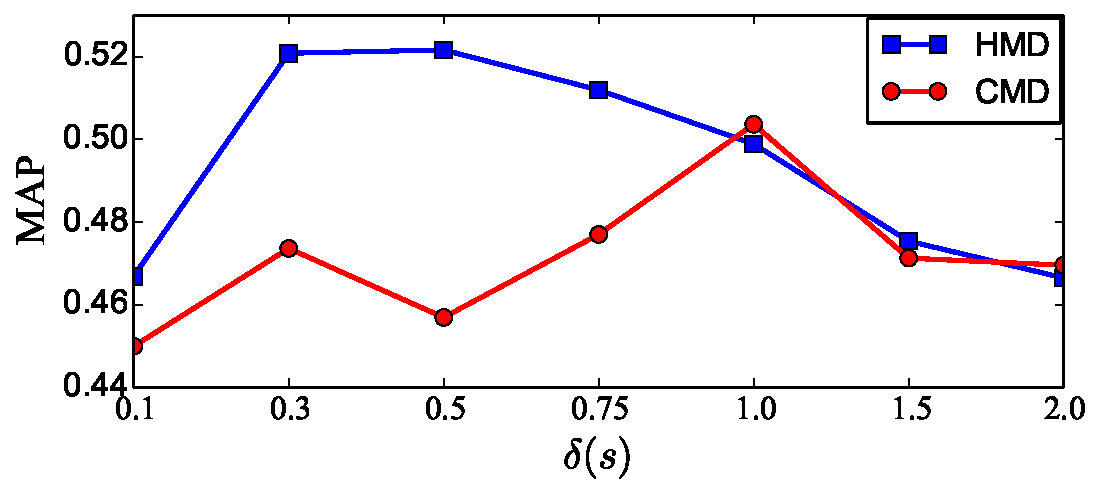
\includegraphics[width=\figSizeEightyFive]{ch06_patterns/figures/ImprovingSimilarity/MAP_per_Duration_Truncation.pdf}
	\end{center}
	\caption[\acrshort{map} score for different duration truncation values]{\gls{map} scores for different duration truncation values ($\svarTruncThsld$) for the \acrshort{msds_cm_hmd} and the \acrshort{msds_cm_cmd}.\TODO{This figure uses symbol, check if it matches the text}} 
	\label{fig:map_per_duration_truncation}
\end{figure}

\begin{figure}
	\begin{center}
		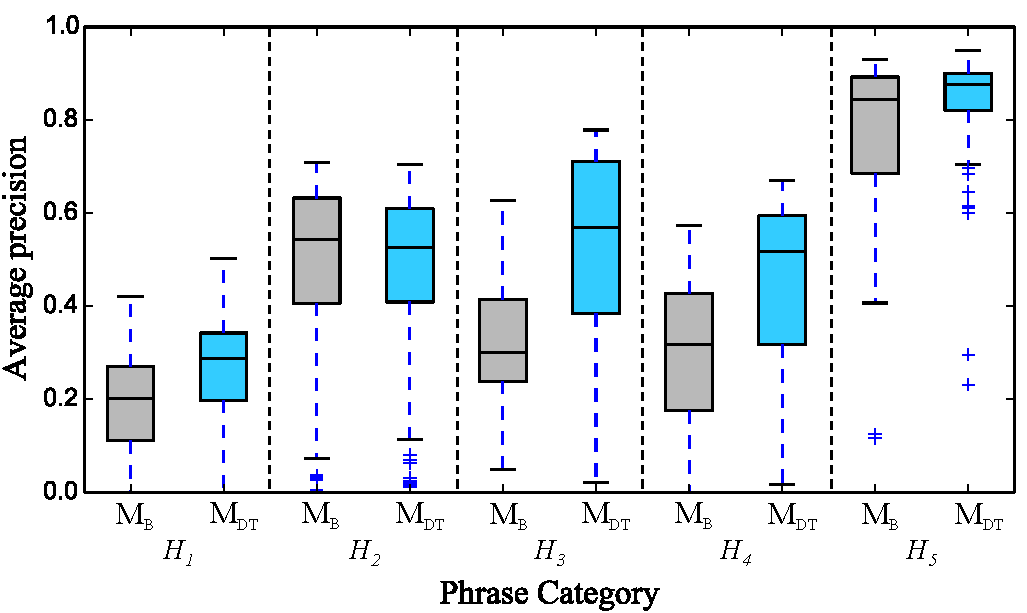
\includegraphics[width=\figSizeEightyFive]{ch06_patterns/figures/ImprovingSimilarity/HindustaniPerCategoryPerformance_BOXPLOT.pdf}
	\end{center}
	\caption[Boxplot of average precision for different types of melodic patterns in the Hindustani music dataset]{Boxplot of average precision values obtained using \acrshort{similarity_b} and \acrshort{similarity_dt} for each melodic phrase category for the \acrshort{msds_cm_hmd}. These values correspond to $\mNorm_\mathrm{tonic}$.\TODO{This figure uses symbol, check if it matches the text}} 
	\label{fig:hinudstaniPerCategoryPerformance}
\end{figure}


We now analyse the results for the \acrshort{msds_cm_cmd} dataset. From~\tabref{tab:patterns_improving_similarity_map_scores} (lower half), we see that using the method variants \acrshort{similarity_dt}, \acrshort{similarity_cw1} and \acrshort{similarity_cw2} we obtain reasonably higher \gls{map} scores compared to the baseline method \acrshort{similarity_b} and the difference is found to be statistically significant for each method variant across all normalization techniques. This \gls{map} score for \acrshort{similarity_dt} corresponds to $\svarTruncThsld=$1\,s, which is considerably higher than the \gls{map} scores for other $\svarTruncThsld$ values as shown in~\figref{fig:map_per_duration_truncation}. We also see that \acrshort{similarity_cw2} performs slightly better than \acrshort{similarity_cw1} and the difference is found to be statistically significant only in the case of $\mNorm_\mathrm{tetra}$. We do not find any statistically significant difference in the performance of methods \acrshort{similarity_dt} and \acrshort{similarity_cw2}. Unlike in the case of the \acrshort{msds_cm_hmd} dataset, for the \acrshort{msds_cm_cmd} dataset $\mNorm_\mathrm{tetra}$ results in the best performance with a statistically significant difference compared to the other normalization techniques across all method variants. We now analyse the average precision values for every phrase category for \acrshort{similarity_b}, \acrshort{similarity_dt} and \acrshort{similarity_cw2}. Since \acrshort{similarity_cw2} performs slightly better than \acrshort{similarity_cw1} we only consider \acrshort{similarity_cw2} for this analysis. In~\figref{fig:carnaticPerCategoryPerformance} we see that \acrshort{similarity_dt} performs better than \acrshort{similarity_b} for all phrase categories.  We also observe that \acrshort{similarity_cw2} consistently performs better than \acrshort{similarity_b} with the sole exception of $C_2$. This exception occurs because \acrshort{similarity_cw2} presumes a consistency in terms of the number of saddle points across the occurrences of a melodic phrase, which does not hold true for $C_2$. This is because phrases corresponding to $C_2$ are rendered very fast and the subtle pitch movements are not the characteristic aspect of such melodic phrases. Hence, the artists often take the liberty of changing the number of saddle points. 

\begin{figure}
	\begin{center}
		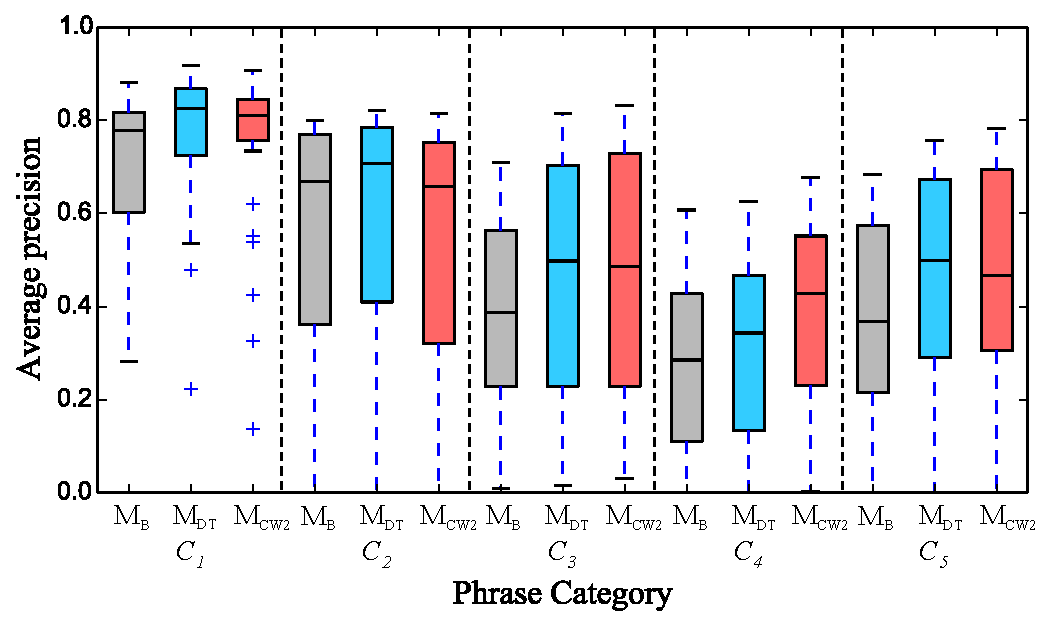
\includegraphics[width=\figSizeEightyFive]{ch06_patterns/figures/ImprovingSimilarity/CarnaticPerCategoryPerformance_BOXPLOT.pdf}
	\end{center}
	\caption[Boxplot of average precision for different types of melodic patterns in the Carnatic music dataset]{Boxplot of average precision values obtained using methods \acrshort{similarity_b}, \acrshort{similarity_dt} and $M_{CW}$ for each melodic phrase category for the \acrshort{msds_cm_cmd}. These values correspond to $\mNorm_\mathrm{tetra}$.\TODO{This figure uses symbol, check if it matches the text}}
	\label{fig:carnaticPerCategoryPerformance}
\end{figure}


Overall, we see that duration truncation of steady melodic regions improves the performance in both \acrshort{msds_cm_hmd} and \acrshort{msds_cm_cmd} datasets. This reinforces our hypothesis that elongation of steady \gls{svara} regions (up to a permissible limit) in the melodies of \gls{iam} in the context of the characteristic melodic phrase does not change the musical identity of the phrase. This correlates with the concept of \gls{nyas} \gls{svara} (\secref{sec:backgroung_nyas_description}), where the artist has the flexibility to stay and elongate a single \gls{svara}. A similar observation was reported in~\cite{Rao2014}, where the authors proposed to learn the optimal global \gls{dtw} constraints a priori for each pattern category. However, as they report, their proposed solution could not improve the performance. Further comparing the results for the \acrshort{msds_cm_hmd} and \acrshort{msds_cm_cmd} datasets we notice that $\mNorm_\mathrm{tonic}$ results in the best performance for the \acrshort{msds_cm_hmd} and $\mNorm_\mathrm{tetra}$ for the \acrshort{msds_cm_cmd}. This can be attributed to the fact that the number of the pitch-transposed occurrences of a melodic phrase is significantly higher in the \acrshort{msds_cm_cmd} compared to the \acrshort{msds_cm_hmd} (\secref{sec:patterns_melodic_similarity_results_discussions}). Also, since the non-linear timing variability in the \acrshort{msds_cm_hmd} is very high, any normalization ($\mNorm_\mathrm{mean}$ or $\mNorm_\mathrm{tetra}$) that involves a decision based on the mean frequency of the phrase is likely to fail.


%################################################################################################################
%########################################### Melodic Pattern Discovery ##########################################
%################################################################################################################


\section{Melodic Pattern Discovery}
\label{sec:patterns_melodic_pattern_discovery}

As argued in \secref{sec:patterns_introduction} the potential of a pattern-based melodic analysis in characterization of \glspl{raga}, compositions and artists  in \gls{iam} gets severely restricted in a supervised experimental setup. As described before, this is mainly due to the factors such as limited dataset size, knowledge bias and human errors in the melodic pattern corpus provided by domain experts. Therefore, to overcome these issues we follow an unsupervised methodology to discover melodic patterns in sizable audio music collections of \gls{iam}. Since a quantitative evaluation of an unsupervised method for sizable datasets is difficult and rather ill-defined, improving such methods and learning optimal values of the system parameters becomes a challenging task. We therefore studied the computation of melodic similarity, a crucial component in a melodic pattern discovery method in a supervised manner in \secref{sec:patterns_evaluation_of_similarity_measures} and \secref{sec:patterns_improving_melodic_similarity}. The learnings from these supervised studies loop back into our unsupervised melodic pattern discovery method presented in this chapter. 

From our literature review presented in \secref{sec:background_relevant_work_other_music} and \secref{sec:background_relevant_work_iam} we see that several approaches have been proposed for extracting different kinds of repeating structures in music, including long-duration repetitions such as different sections of a music piece~\citep{serra2012unsupervised,Goto06TASLP, paulus2010state}, relatively small-duration repetitions being themes, riffs~\citep{Hsu2001a}, and melodic motifs~\citep{meredith2002algorithms,collins2011improved,Janssen2013}. While there exists a number of approaches for motivic discovery in sheet music~\citep{meredith2002algorithms,Cambouropoulos2006,conklin2001representation,Lartillot2005}, there are fewer approaches that work on audio music recordings~\citep{dannenberg2003pattern}. This can be attributed to the audio-symbolic gap \citep{collins2014bridging}, which is argued to be bridged by a reliable automatic transcription system to abstract the audio music content into musically meaningful discrete symbols. Although, for several music traditions such as \gls{iam} melodic transcription still remains a challenging and a rather ill-defined task.  A detailed account of the shortcomings in the existing pattern discovery methods in the context of their applicability to melodies in \gls{iam} is presented in our literature review in \secref{sec:sota_pattern_processing_iam} and \secref{sec:query_by_humming}. We see that there exists a wide scope for developing methodologies for the discovery and analysis of short duration melodic patterns (or motifs) in large audio music collections. Approaches for motif discovery can benefit from the literature in the domain of time series analysis such as time series representation~\citep{Lin2003}, core pattern discovery methods~\citep{Mueen2009}, and search and indexing techniques~\citep{Rakthanmanon2013}. We now proceed to describe our methodology for melodic pattern discovery in sizable audio music collections of \gls{iam}.


\subsection{Method}
\label{sec:patterns_discovery_method}

\begin{figure}
	\begin{center}
		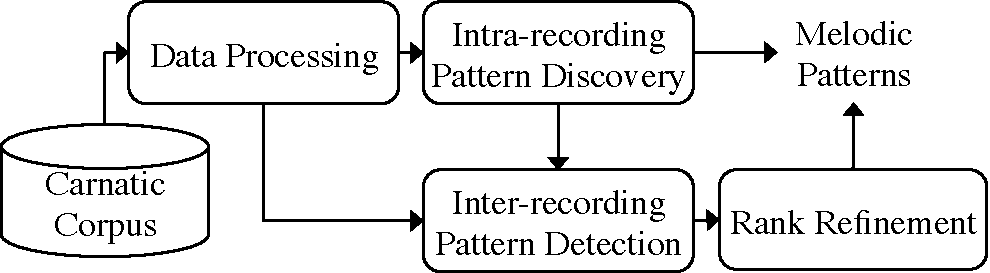
\includegraphics[width=\figSizeEightyFive]{ch06_patterns/figures/discovery/blockDiagram_Overall.pdf}
	\end{center}
	\caption[Block diagram for melodic pattern discovery]{Block diagram of the proposed approach for melodic pattern discovery in large audio collections of \gls{iam}\TODO{Carnatic->IAM}}
	\label{fig:pattern_discovery_overall_block_diagram}
\end{figure}

Our approach consists of four main blocks as shown in~\figref{fig:pattern_discovery_overall_block_diagram}. The data processing block generates pitch subsequences from every audio recording in the music collection, which are potential pattern candidates. The intra-recording pattern discovery block performs an exact pattern discovery by detecting the closest subsequence pairs within an audio recording (referred to as seed patterns). The inter-recording pattern detection block considers each seed pattern as a query and searches for its occurrences in the entire music collection. The rank refinement block reorders a ranked list of search results by recomputing melodic similarity using a more sophisticated similarity measure. The following description is based on our work presented in~\cite{gulati_SITIS_2014}.

We choose to perform first an intra-recording pattern discovery because melodic patterns are repeated within a music piece in \gls{iam}. Moreover, the scalability of the computational approaches considered here for discovering patterns at the level of the entire music collection is questionable. To confirm this hypothesis, we conducted an experiment using a state-of-the-art algorithm for time series motif discovery~\citep{Mueen2009}, with a trivial modification to extract the top K motifs. Using just 16\,hours of audio data (amounting to around 20\,million pitch samples), the algorithm could discover only 40~melodic patterns in 24\,hours using Euclidean distance. Besides pattern pairs being from the same recording, only a few of the obtained pattern pairs were melodically similar and meaningful. This is expected as we found in \secref{sec:patterns_melodic_similarity_results_discussions} that Euclidean distance is not appropriate for handling large-non linear timing variations present across occurrences of melodic patterns. In order to scale pattern discovery for hundreds of hours of audio data using a computationally complex \gls{dtw}-based distance measure we choose to first perform pattern discovery within an audio recording.

Before we proceed to describe our method it should be noted that during the course of this dissertation several processing blocks and system parameters presented in the subsequent sections have evolved. The methodology presented in this section is based on our work reported in~\cite{gulati_SITIS_2014}. However, after that study, based on our findings in ~\cite{gulati_ICASSP2015} and in~\cite{gulati_ICASSP2015} we have modified the procedure followed in several processing blocks and system parameters. In order to facilitate reproducibility of our experiments and research outcomes, along with the original description of the method~\citep{gulati_SITIS_2014} we also present the modifications done for the new (the most recent) variant of the method. Wherever applicable the modifications are presented during the description of the processing block. Since the evaluation methodology we followed involve cumbersome listening tests, the results presented in this section are only corresponding to the initial variant of the method presented in~\cite{gulati_SITIS_2014}.


\subsubsection{Pre-processing}
\label{sec:pattern_discover_preprocessing}

\begin{figure}
	\begin{center}
		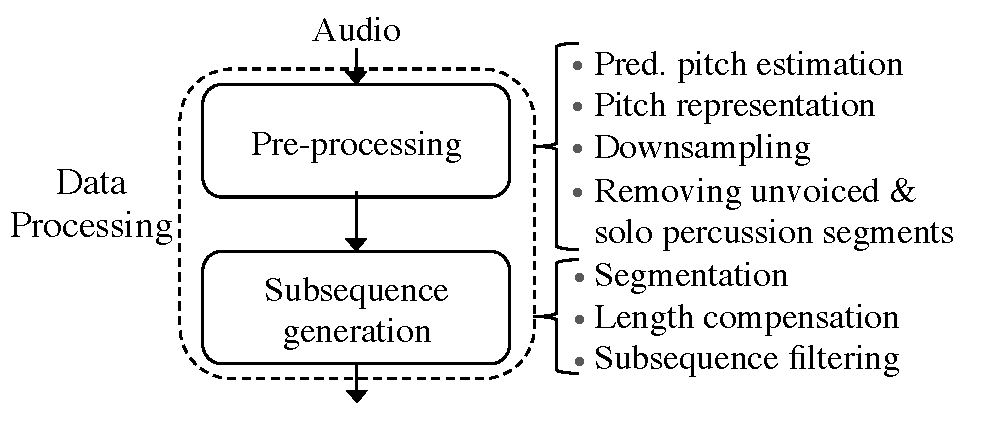
\includegraphics[width=\figSizeEightyFive]{ch06_patterns/figures/discovery/blockDiagram_DataProc.pdf}
	\end{center}
	\caption[Block diagram of data processing modules for melodic pattern discovery]{Block diagram of the data processing block in melodic pattern discovery task.}
	\label{fig:pattern_discovery_preprocessing_block_diagram}
\end{figure}


The steps involved in the pre-processing block are shown in Fig.~\ref{fig:pattern_discovery_preprocessing_block_diagram}. A description of each of these steps is given below:

\paragraph{a) Predominant Pitch Estimation and Representation} 

We consider melody as the predominant pitch in the audio signal. For estimating predominant pitch we follow the procedure we used in~\secref{sec:patterns_evaluation_of_similarity_measures}, which is described in detail in~\secref{sec:data_preprocessing_predominant_melody_estimation}. We use a frame size of 46\,ms and a hop size of 4.44\,ms. Noticeably, the predominant pitch estimation method that we use also performs voicing detection, which is used in the later part of our data processing methodology to filter unvoiced segments (\figref{fig:pattern_discovery_preprocessing_block_diagram}). We do not perform any post-processing on the estimated pitch contours.

For the melody representation to be musically relevant, the pitch values are converted from Hertz to Cents (\secref{sec:data_processing_cent_conversion}). In order to compare melodies across different artists and recordings we additionally consider the tonic pitch of the lead artist in the recording as the reference frequency during this conversion. The tonic of the lead artist for each recording in the collection is identified automatically using \acrshort{tonicid_justin} method, which is found to be the best performing method for this task in our comparative evaluation~(\secref{sec:data_preprocessing_tonic_identification}).

In the new variant of our method we post-process the predominant pitch contours as described in~\secref{sec:data_preprocessing_pitch_postprocessing}. We perform median and Gaussian filtering to remove spurious pitch jumps lasting over a few samples and to smooth the pitch contours. In addition, we also interpolate short non-voiced segments that usually correspond to intra-phrase breath pauses or to consonants in the lyrics (\secref{sec:data_processing_pitch_interpolation}). 


\begin{figure}
	\begin{center}
		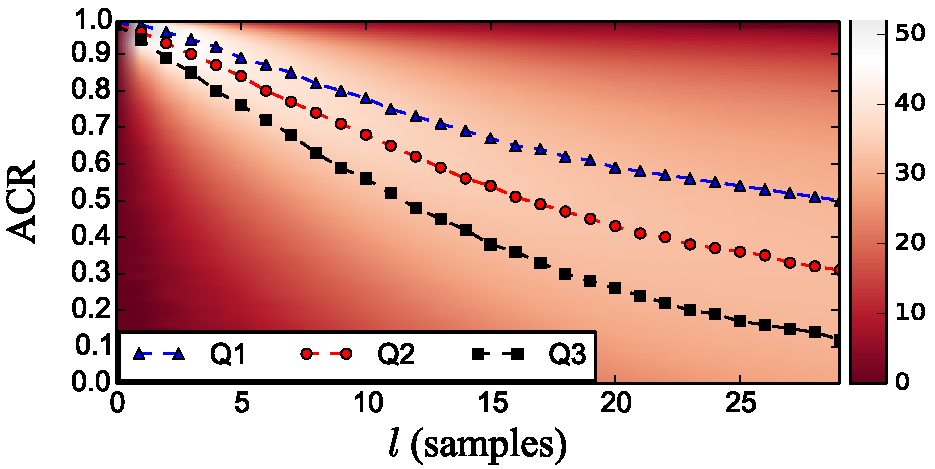
\includegraphics[width=\figSizeEightyFive]{ch06_patterns/figures/discovery/ACRHistogram.pdf}
	\end{center}
	\caption[Histogram of autocorrelation of the pitch subsequences for different lags]{Histograms of ACR values (histogram value is indicated by the colormap on the right; for ease of visualization, we compress the range of the histogram values by taking its fourth root). Q1, Q2 and Q3 denote the three quartile boundaries of the histogram. }
	\label{fig:ACRHistogram}
\end{figure}


\paragraph{b) Downsampling} 
As mentioned above, we estimate predominant pitch at a sampling rate of around 225\,Hz. However, in order to reduce the computational cost, we downsample the predominant pitch sequence~(\figref{fig:pattern_discovery_preprocessing_block_diagram}). We could not find any study that systematically reports the effect of sampling rate on melodic similarity in \gls{iam}\footnote{Note that the current study was performed before our supervised studies presented in~\secref{sec:patterns_evaluation_of_similarity_measures} and \secref{sec:patterns_improving_melodic_similarity}, where we analyze the influence of sampling rate on melodic similarity.}. In such a case, we derive an optimal sampling rate by analyzing the autocorrelation (ACR) of short-time pitch segments generated using a sliding window of 2\,s. We compute the ACR of all possible pitch segments in the entire dataset for different lags $l$, $l\in \lbrace0,1,\dots30\rbrace$, and examine the histogram of normalized ACR values at each lag (\figref{fig:ACRHistogram}). We select the lag at which the third quartile Q3 has an ACR value of 0.8, which corresponds to a sampling rate of 22.22\,ms~(or 45\,Hz). We informally found that this sampling rate generally preserves melodic nuances and rapid pitch movements in Carnatic music while reducing the computational requirements of the task. Note that in the new variant of our method, we use the optimal sampling rate derived from our comprehensive quantitative evaluations in~\cite{gulati_ICASSP2015} (see~\secref{sec:patterns_evaluation_of_similarity_measures}). %We use a sampling rate of 56\,Hz for Carnatic music and 45\,Hz for Hindustani music.  


%Note that the study in this section was originally presented in~\cite{gulati_SITIS_2014} and was conducted before we quantitatively assessed the optimal parameter settings in~\cite{gulati_ICASSP2015} (see~\secref{sec:patterns_evaluation_of_similarity_measures}). In the subsequent studies  Although, the heuristically chosen sampling rate in this study is not drastically different from the optimal sampling rate reported in~\cite{gulati_ICASSP2015} (see \TODO{Figure(where we show the accuracy vs sampling rate)}). 


\paragraph{c) Solo Percussion Removal} 

As described in \secref{sec:pre_processing_tani_segmentation}, a concert of Carnatic music typically contains a solo percussion section, referred to as a \gls{tani} section, which can last up to 2-25\,minutes. We find that the predominant pitch estimation method employed in this study often tracks pitch corresponding to the \gls{mridangam} strokes instead of detecting \gls{tani} sections as non-voiced segments. This poses a challenge for melodic pattern discovery as there are several repeating percussion patterns in \gls{tani} sections, which are often discovered as the closest melodic pattern pairs. In \secref{sec:pre_processing_tani_segmentation}, we explain this issue in detail and describe a classification-based approach to detect \gls{tani} sections in audio recordings of Carnatic music. Once detected, we can simply discard the pitch samples corresponding to these sections and overcome the challenge. In addition to avoiding the unwanted melodic patterns being present in the output, by discarding the \gls{tani} sections we also reduce the computational complexity of our method.


\subsubsection{Subsequence Generation}
\label{sec:subsequencegeneration}

In this processing block we generate melodic pattern candidates from the resultant pitch representation~(\figref{fig:pattern_discovery_preprocessing_block_diagram}). The steps involved in generating candidate subsequences are described below.

\paragraph{a) Segmentation} 

As seen in~\secref{sec:patterns_melodic_similarity_results_discussions}, an accurate segmentation of melodic patterns has a big impact on the computation of melodic similarity, and eventually on the retrieval accuracy of melodic patterns. In the literature (\secref{sec:motif_in_symbolic_music}) there are several models studied for melodic segmentation~\citep{Cambouropoulos2006,muller2009robust,cambouropoulos2001local}. \cite{pearce2008comparison} and \cite{rodriguez2014comparing} provide a comparison of a number of such models. However, none of these models is directly applicable on the continuous melody representation we use for \gls{iam}. Due to the lack of such studies and reliable models for segmentation of melodic patterns in \gls{iam}, we use a brute-force approach for generating pattern candidates. We generate candidate pitch subsequences by using a sliding window of length $\pattLenSec$ with a hop size of one sample. Given no quantitative studies investigating the length of the melodic patterns in \gls{iam}, we make a choice of $\pattLenSec = 2$\,s based on recommendations from a few professional musicians.

Since unvoiced segments are removed from the pitch sequence at the pre-processing step~(\figref{fig:pattern_discovery_preprocessing_block_diagram}), a pattern candidate can include pitch samples separated by more than $\pattLenSec$ seconds. To handle these cases, we use the time stamps of the first sample ($\timeStamp_1$) and the last sample ($\timeStamp_2$) in the subsequence. We filter out all subsequences for which $\timeStamp_2-\timeStamp_1 > \pattLenSec + \shortPauseDur$. We select $\shortPauseDur =0.5$\,s to account for the short pauses during a phrase rendition. This value was empirically set to differentiate between inter- and intra-phrase pauses. 

In the new variant of our method, the processing step described in the previous paragraph becomes redundant, and is therefore not applied. Since in this variant the short-duration unvoiced regions in the predominant pitch contours are interpolated, there will not be any situation where $\timeStamp_2-\timeStamp_1 > \pattLenSec + \shortPauseDur$. 


\paragraph{b) Subsequence Filtering} 

One of the challenges in melodic pattern discovery is the presence of combinatorial redundancy in the form of musically trivial patterns in the output~\citep{Lartillot2005}. One such redundancy in our case is that of a melodic pattern comprising a single \gls{svara}. Instead of removing such musically uninteresting patterns after they are discovered, we detect and discard such subsequences (or pattern candidates) during the pre-processing step (\figref{fig:pattern_discovery_preprocessing_block_diagram}). The criterion for discarding such subsequences is summarized below:

\begin{equation}
\label{eq:flatness_measure}
\flatMeas =\sum_{i=0}^{\pattLenSym} \heaviside\left(\stdDevSubSeq_i\geq \stdDevThsld\right),
\end{equation}


\noindent where $\flatMeas$ is the flatness measure of a subsequence, $\pattLenSym$ denotes its number of samples, $\heaviside(z)$ is a Heaviside step function yielding $\heaviside(\text{true})\!=\!1$ and $\heaviside(\text{false})\!=\!0$, and $\stdDevSubSeq_i$ is the standard deviation at the $i$-th sample of a subsequence, computed using a window of length $\stdDevWin$ centered at sample $i$. The threshold $\stdDevThsld$ determines if a sample belongs to a flat region or not. In order to determine the optimal values of $\stdDevWin$ and $\stdDevThsld$, we manually labeled a number of regions in pitch contour as `flat' and `non-flat' for 4 excerpts in our database. We iterated over different parameter values and analyzed the resultant ROC curve shown in~\figref{fig:ROC_pattern_discovery}). %In  we show the ROC curve obtained for $\stdDevWin \in \lbrace100,200,400\rbrace$\,ms. 
Doing so, we found that $\stdDevWin=200$\,ms resulted in the best performance and that the knee of the curve corresponded to $\stdDevThsld=45$\,Cents. Having a value of $\flatMeas$ for each subsequence, we finally filter out the ones for which $\flatMeas \leq \flatThsld \pattLenSym$, using $\flatThsld = 0.8$. The latter was set by visual inspection.

\begin{figure}
	\begin{center}
		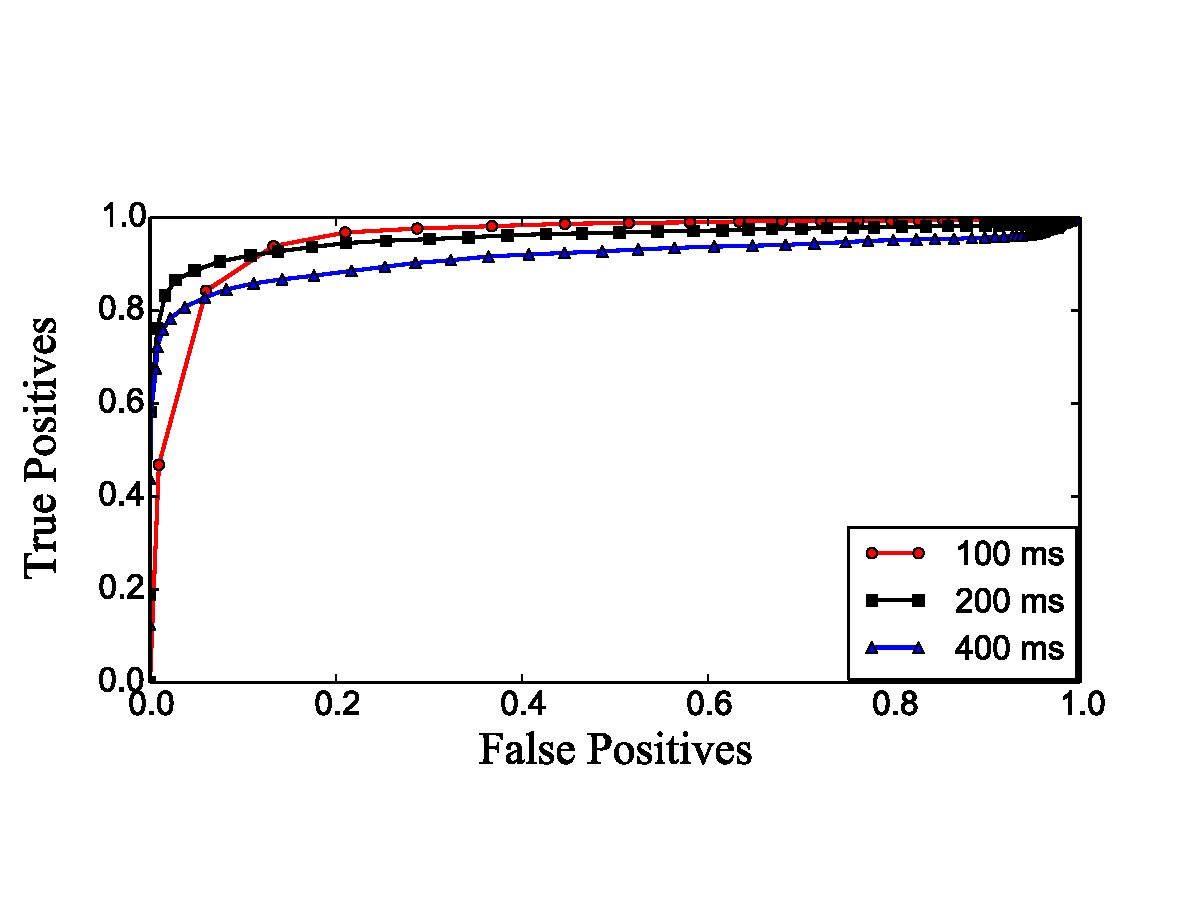
\includegraphics[width=\figSizeEightyFive]{ch06_patterns/figures/discovery/ROCFlatness.pdf}
	\end{center}
	\caption[ROC curve for `flat' and `non-flat' region classification]{ROC curves for `flat' and `non-flat' region classification for different values of window length ($\stdDevWin$) used for selecting an optimal value of standard deviation $\stdDevSubSeq_i$.}
	\label{fig:ROC_pattern_discovery}
\end{figure}

In the new variant of our pattern discovery method, we use the segmentation approach described in~\secref{sec:nyas_svara_segmentation_method} to detect the stable \gls{svara} regions in melodies. The pitch samples in a subsequence that correspond to these stable \gls{svara} regions are regarded as `flat', which is analogous to $\stdDevSubSeq_i\geq \stdDevThsld$ being `True' for those samples. All other parameters remain the same as described above. This change is done because the segmentation approach produces more reliable estimates of the stable melodic regions compared to the simple measure using local standard deviation of the pitch samples. 

 %In the current study our dataset comprises only Carnatic music. For Hindustani music the reduction ratio of number of pattern candidates might be even higher due to the presence of long held \gls{svaras}.

\subsubsection{Intra-recording Pattern Discovery}
\label{sec:intraRecordingPatternDiscovery}

In this step our aim is to discover melodic patterns within each recording in the audio collection. We perform an exact pattern discovery by computing the similarity between every possible subsequence pair obtained within an audio recording. Thus, the computational complexity of this task is quadratic ($\bigO(n^2)$) over the number of subsequences. We regard the top $\topKIntra=25$ closest subsequence pairs in each recording as seed patterns. We omit overlapping subsequences in order to avoid trivial matches and additionally constrain the top $\topKIntra$ seed pattern pairs to be mutually non-overlapping. Due to this constraint for some recordings we obtain less than 25 pattern pairs. 


\paragraph{Melodic Similarity} 

We compute melodic similarity between two subsequences using a \gls{dtw}-based distance measure (\secref{sec_DTW_distance_measure}). This choice is supported by our findings in~\secref{sec:patterns_melodic_similarity_results_discussions}, wherein we showed that a \gls{dtw}-based distance measure outperforms Euclidean distance measure in melodic similarity computation in \gls{iam}. We use a step condition of $\lbrace(1,0), (1,1), (0,1)\rbrace$ and the squared Euclidean distance as the cost function. The accumulated cost matrix for this step condition is computed as described in \eqnref{eq:dtw_classic_cost_matrix_computation}. We do not use any penalty for insertion and deletion. In addition, we apply the Sakoe-Chiba global constraint with the band width set to 10\% of the pattern length. This constraint was found to be sufficiently large for accounting time warpings in melodic repetitions in Carnatic music (see \tabref{tab:melodic_similarity_results}). For the case of Hindustani music, an unconstrained \gls{dtw} variant is shown to perform the best. However, to make the system computationally tractable we finally choose 10\% band width for both the music traditions. Notice that these parameter values are close to the optimal settings but not the most optimal settings for a \gls{dtw} variant that we obtained in \secref{tab:melodic_similarity_results}. We make these compromises in order to avail lower bounding techniques as explained in the subsequent sections. 	

\paragraph{Lower Bounding \gls{dtw}}
\label{LowerBoundingDTW}

The computational complexity of a brute-force pattern discovery system using a \gls{dtw} distance measure is quadratic ($\bigO(n^2)$) over both the number of subsequences and the length of a subsequence. For a dataset as big as ours that contains millions of subsequences (pattern candidates), where the length of each subsequence is around 100\,samples, the system becomes extremely demanding in terms of the CPU time. Even after reducing the number of pattern candidates by filtering out subsequences in the pre-processing step and reducing the length of the subsequences by downsampling the pitch representation, it is not practically feasible to perform the task. One of the ways to address this problem is to use indexing or lower bounding techniques with which we can prune subsequence pairs that can not possibly be the best matches. Pruning of the subsequence pairs reduces the number of times the \gls{dtw} computation is done, and thus make \gls{dtw} distance computations tractable for datasets with large number of subsequences.

In literature there are several methods proposed for indexing the \gls{dtw} distance~\citep{Keogh2004,vlachos2003indexing,kim2001index}. These methods differ in terms of their computational complexities and the type of indexing techniques they employ (approximate or exact). In this study to speed up \gls{dtw} computations we use the exact \gls{dtw} indexing technique~\citep{Keogh2004} and apply cascaded lower bounds as explained in~\cite{Rakthanmanon2013}. This method is parameter free, it does not require any pre-processing of the data and there is no constraint on the minimum and maximum query length. In particular, we use \acrshort{lbKIMFL} (first-last) lower bound~\citep{kim2001index} and \acrshort{lbKeogh} bound~\citep{Keogh2004} for both query to reference and reference to query matching (denoted by \acrshort{lbKeoghEQ} and \acrshort{lbKeoghEC}, respectively). In \acrshort{lbKeoghEQ} lower-bounding envelopes are computed for the query pattern, and in \acrshort{lbKeoghEC}, they are computed for the reference. Besides, we apply early abandoning, both during the computation of lower bounds as well as during the \gls{dtw} distance computation. These lower bounding techniques are explained in~\secref{sec:background_lowerbound}, however, for a more detailed explanation we refer to~\cite{Rakthanmanon2013}. 

In \algoref{alg:algorithmdiscovery} we show the pattern discovery routine that uses cascaded lower bounds to speed up \gls{dtw}. This pseudo-code provides a better understanding of the pruning procedure and puts in context the utility of using different lower bounds. Note that in this routine we show the discovery of only the closest subsequence pair. With a trivial addition of incorporating a priority queue that stores the K most closest subsequence pairs at each step, we extend it to our use-case of discovering the top K closest melodic patterns. We further optimize this routine by pre-computing the subsequence envelopes used in the computation of LB\_Keogh bound (\secref{sec:background_lowerbound}).

\renewcommand{\algorithmiccomment}[1]{\bgroup\hfill\tiny//~#1\egroup}
\begin{algorithm}
\caption{Discovering the closest subsequence pair using the \gls{dtw} distance and cascaded lower bounds.}
\label{alg:algorithmdiscovery}
	\begin{algorithmic} 
	
	\State {\bf Input:} array $\patternArray$ containing $N$ number of subsequences
	\State \texttt{best\_so\_far} = \texttt{infinity};
	\For{$i$=0; $i \leq N-1$; $i$++}
		\For{$j$=0; $j \leq N-1$; $j$++}
			\State  \texttt{dist\_FL} = \texttt{\acrshort{lbKIMFL}($\pattern_i$, $\pattern_j$)}			
			\If {\texttt{dist\_FL} < \texttt{best\_so\_far}}				
				\State  \texttt{dist\_EQ} = \texttt{LB\_Keogh($\pattern_i$, $\pattern_j$)}				
				\If {\texttt{dist\_EQ} < \texttt{best\_so\_far}}				
					\State  \texttt{dist\_EC} = \texttt{LB\_Keogh($\pattern_j$, $\pattern_i$)}					
					\If {\texttt{dist\_EC} < \texttt{best\_so\_far}}					
						\State  \texttt{true\_dist} = \texttt{DTW($\pattern_i$, $\pattern_j$)}						
						\If {\texttt{true\_dist} < \texttt{best\_so\_far}}
							\State \texttt{best\_so\_far} = \texttt{true\_dist}
							\State \texttt{closest\_pair\_index} = ($i$,$j$)							
						\EndIf
					\EndIf
				\EndIf
			\EndIf
		\EndFor
	\EndFor
	
	\end{algorithmic}
\end{algorithm}
				

\paragraph{Pattern Length Compensation}
\label{PatternLengthCompensation}

Along with the local non-linear time warpings, the overall length of a melodic pattern may also vary across repetitions. For example, a melodic pattern of length 2\,s might be sung in 2.2\,s in a different position in the recording. We handle this by using multiple time scaled versions of a subsequence in the distance computation. 
Performing appropriate uniform time-scaling prior to \gls{dtw} is known to produce tighter lower bounds~\citep{Zhu2003}, which is similar to a technique referred to as local \gls{dtw}. It should be noted that such timing variations could as well be addressed by using a subsequence variant of \gls{dtw}. However, the lower bounding techniques we use to speed up the \gls{dtw} distance computation do not work for the subsequence variant of the \gls{dtw}. 

For every subsequence, we generate five subsequences by uniformly time scaling it by a factor of $\timeScaFac \in \lbrace 0.9, 0.95, 1, 1.05, 1.1\rbrace$, such that the length of the resulting subsequences is $\pattLenSec$. We use cubic interpolation for uniformly time scaling a subsequence. Creating five uniform time scaled subsequences for each subsequence increases the computational cost by a factor of 25. We observe that the distance between a subsequence pair $X_{1.0}$ and $Y_{1.05}$ is very close to the distance between the pair $X_{1.05}$ and $Y_{1.1}$ (the sub-index denotes the interpolation factor $\timeScaFac$). Thus by following this rationale and using this approximation, we can avoid the distance computation between 16 of the 25 combinations without a significant compromise on accuracy. We only retain the combinations for which the difference between the interpolation factors of subsequence pairs are unique. \COMMENT{Figure?? matrix if time permits}

\subsubsection{Inter-recording Pattern Detection}
\label{sec:inter_recording_pattern_search}

After discovering melodic patterns within each audio recording, we now proceed to detect their occurrences in all the recordings in the collection. For this, we consider every seed pattern as a query and perform an exhaustive search over all the subsequences obtained from the entire audio music collection. For every seed pattern we store top $\topKInter=200$ closest matches (referred to as search patterns). To avoid redundancy in the search results, we constrain search patterns for every seed pattern to be mutually non-overlapping. Similar to the intra-recording pattern discovery step, here also for every subsequence we consider 5 uniformly  time scaled subsequences in the distance computation. Furthermore, for detecting occurrences of seed patterns in other recordings we use the same similarity measure and lower bounding techniques as used in Intra-recording pattern discovery. The pattern detection routine is a small modification of the routine shown in~\algoref{alg:algorithmdiscovery}. Instead of a single subsequence array, we would have two arrays; one of which comprises the seed patterns (queries) and the other comprises subsequences obtained from all the recordings (target candidates). 

\subsubsection{Rank Refinement}
\label{sec:rankRefinement}

As mentioned before, the lower bounds used for speeding up the distance computations are not valid for any variant of the \gls{dtw} distance. This constraint governed the choices made for the \gls{dtw} variant and the parameter settings for computing melodic similarity in both the intra and the inter-recording pattern processing blocks. However, once the top matches are found, nothing prevents us from reordering the ranked list using any variant of the \gls{dtw} distance. This is because the number of top matches we consider ($\topKInter=200$) per query is orders of magnitude smaller than the total number of subsequences obtained from the entire audio collection. For every query pattern, we now recompute the melodic similarity with its top \topKInter search patterns using a more robust and a better performing variant of the \gls{dtw} distance.

During rank refinement, we select a \gls{dtw} step condition of $\lbrace(1,2), (1,1), (2,1)\rbrace$ to avoid some pathological warpings of the path. This step condition, which also acts as a local constraint was shown to better model the melodic similarity in~\secref{sec:patterns_melodic_similarity_results_discussions}. Furthermore, we investigate four different distance measures $\dtwCostFnc_i$, $i=1,\dots 4$, used in the computation of the \gls{dtw} cost matrix. These distance measures are described below in~\eqnref{eq:distance_measures_discovery}. For a better understanding of the distance measures we also show them in~\figref{fig:Distances_DTW_discovery}.


\begin{figure}
	\begin{center}
		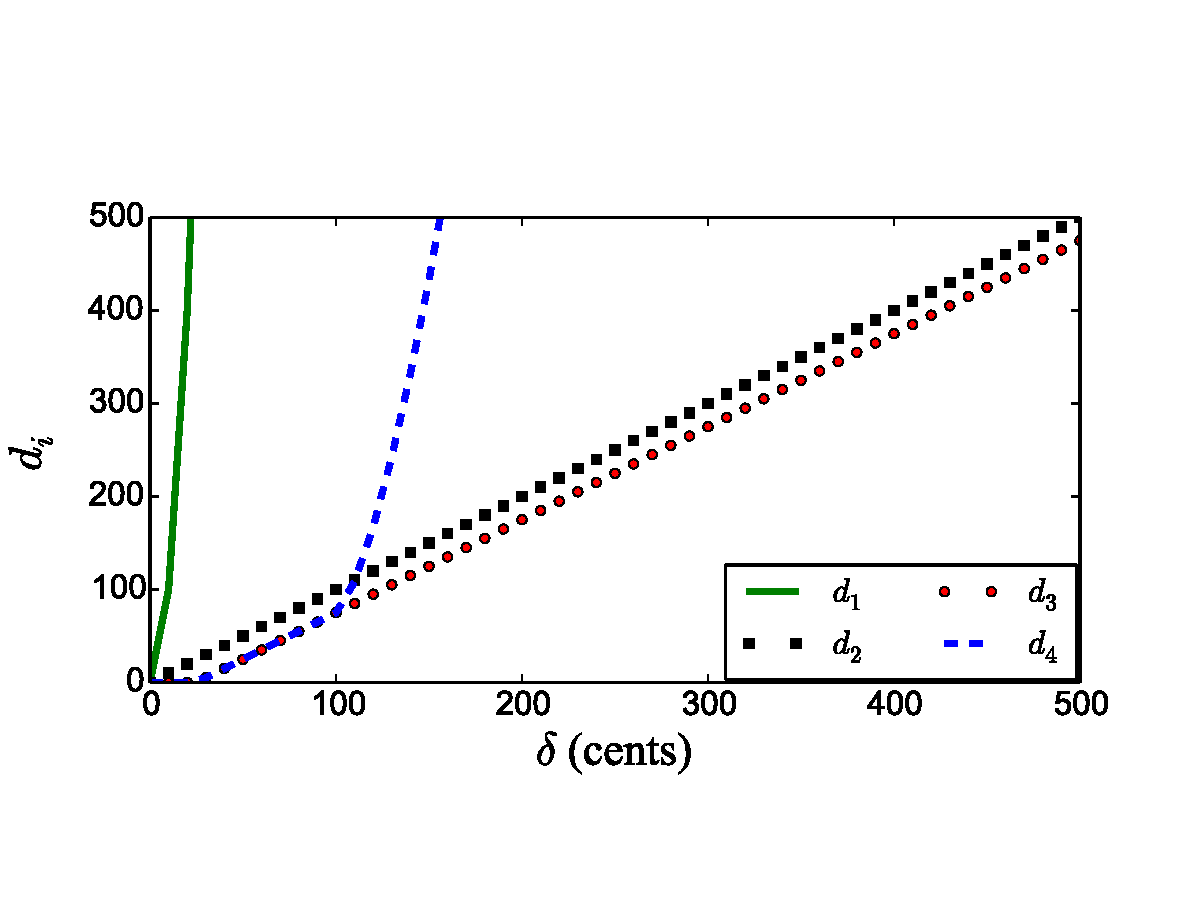
\includegraphics[width=\figSizeEightyFive]{ch06_patterns/figures/discovery/distances.pdf}
	\end{center}
	\caption[Illustration of output of different distance measures]{Output of the four different distance measures ($\dtwCostFnc_i$, $i \in \lbrace 1\cdots4 \rbrace$) as a function of cityblock distance \pitchDiff.\TODO{This figure uses symbol, check if it matches the text}}
	\label{fig:Distances_DTW_discovery}
\end{figure}


\begin{equation}
\begin{aligned}
\dtwCostFnc_1& = \pitchDiff \hspace{.5em}\\
\dtwCostFnc_2& = \pitchDiff^2 \hspace{.5em}\\
\dtwCostFnc_3& = 
\begin{cases}
\pitchDiff-25, & \hspace{1cm} \text{if } \pitchDiff >25\\
0, & \hspace{1cm}\text{otherwise } 
\end{cases}\\
\dtwCostFnc_4 &= 
\begin{cases}
(\pitchDiff-\arbitTshldOne)^{1.5} + \arbitTshldTwo, & \text{if } \pitchDiff >100\\
\dtwCostFnc_3, & \text{otherwise}
\end{cases}
\end{aligned}
\label{eq:distance_measures_discovery}
\end{equation}

\noindent where $\pitchDiff = |\pitchCents_1-\pitchCents_2|$ is the city block distance between two pitch values and all numeric values are in Cent scale. We set $\arbitTshldOne =99.55$ and $\arbitTshldTwo = 74.7$ to maintain point and slope continuity of the function. The formulation for these different distance measures ($\dtwCostFnc_i$) is inspired by our own experience and some of the approaches we find in the literature~\citep{Ishwar2013,Rao2014}. We denote the four variants of the rank refinement method by $\RankRefVar_i$, where $i \in \lbrace 1\cdots4 \rbrace$.


\subsection{Evaluation}

\subsubsection{Music Collection}
\label{sec:pattern_discovery_musiccollection}

The music collection used for studying the task of pattern discovery in this section comprises 365\,hours Carnatic music. It contains 1764 audio recordings, which are carefully compiled as a part of the CompMusic Carnatic music corpus (\secref{sec:corpus_carnatic_music_corpus}). As explained in~\secref{sec:corpus_carnatic_music_corpus}, these audio recordings are ripped from commercially released music CDs. The selected music material is diverse in terms of the number of artists, gender of lead artists, number of different \glspl{raga}, year of release and various forms within Carnatic music.

\COMMENT{If time permits provide statistics of this dataset here as well? they are already talked about in the corpus chapter}


\subsubsection{Evaluation Methodology}
\label{sec:evaluationmethodology}

One of the challenges in an unsupervised data-driven approach such as the one we use for discovering melodic patterns is its evaluation. We here perform a quantitative evaluation based on expert feedback. For the entire dataset we obtain over 15\,million search patterns for each of the rank refinement methods. We divide seed patterns into three categories based on the distance between the seed pairs, which we denote by $\distPatt$. The distribution of the distance $\distPatt$ between the seed pattern pairs is shown in~\figref{fig:SeedPatternsDistanceDistribution}. Then, to have an equal representation from the range of values of $\distPatt$, 200 seed pairs equally distributed among these categories are randomly selected for evaluation. Seed category boundaries are $\mu \pm 1.5\sigma$, where $\mu$ and $\sigma$ are the mean and the standard deviation of the distribution of $\distPatt$. For every selected seed pattern we consider the first 10 search patterns for each of the four rank refinement methods for evaluation. Thus, in total, we obtain 200 seed pairs and 8,000 search patterns for expert evaluation.

Expert evaluation is performed by a professional Carnatic musician who has received over 20 years of music education. For examining similarity between two melodic patterns, the musician listened to the audio fragments corresponding to these patterns and scored a 0 for melodically dissimilar and a 1 for melodically similar pattern. The musician annotated melodic similarity for each seed pair and between the seed and its search patterns for every rank refinement method.


\begin{figure}
	\begin{center}
		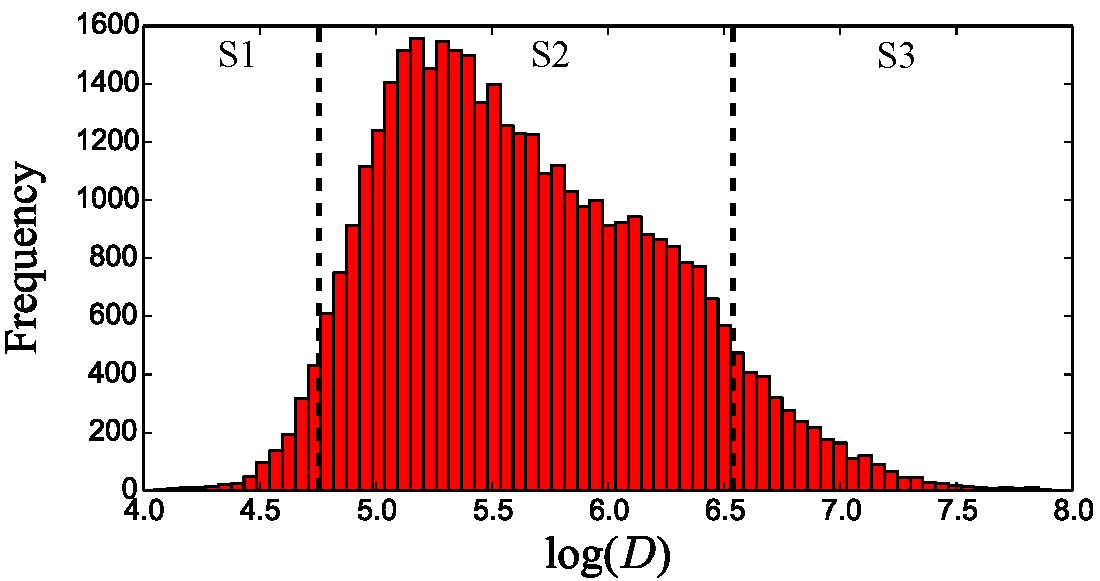
\includegraphics[width=\figSizeEightyFive]{ch06_patterns/figures/discovery/SeedDistribution.pdf}
	\end{center}
	\caption[Distance distribution of seed melodic patterns]{Distance distribution of seed patterns. Three seed pattern categories are marked by $\seedPattCat_1$, $\seedPattCat_2$ and $\seedPattCat_3$.\TODO{This figure uses symbol, check if it matches the text}}
	\label{fig:SeedPatternsDistanceDistribution}
\end{figure}


To quantify the musician's assessment of the similarity between the melodic patterns  we use \gls{map}, a typical evaluation measure in information retrieval~\citep{manning2008introduction}, which is also very common in \gls{mir}. This way, we have a single number to evaluate the performance of the four different rank refinement methods. Since we do not have ground-truth annotations of melodic patterns for our dataset, total number of occurrences of different patterns is unknown. Therefore, while computing the \gls{map} scores we consider the total number of relevant patterns as the number of relevant patterns retrieved in the top 10 search results.  For assessing statistical significance we use the Mann-Whitney U test~\citep{mann1947test} with $\pVal < 0.05$. To compensate for multiple comparisons, we apply the Holm-Bonferroni method~\citep{holm1979simple}. Thus, eventually we use a much more stringent criteria than $\pVal < 0.05$ for measuring statistical significance. We also use ROC curves to analyze the separation between the distance distribution of melodically similar and dissimilar subsequences~\citep{manning2008introduction}. 


\subsection{Results and Discussion}
\label{sec:patterns_discovery_results}

Before presenting the results of the evaluation of the discovered patterns, we provide details in terms of the number of patterns and \gls{dtw} computations done at each step. Our dataset comprising 365\,hours of audio data contains nearly 300\,million pitch samples (considering 225\,Hz as the sampling rate of the pitch contours). In a brute force segmentation scenario that would amount to roughly the same number of pattern candidates. However, since we downsample the pitch contours and filter out musically trivial patterns, we retain around 17.5\,million pattern candidates after data pre-processing step. In the intra-recording pattern discovery block, for all the recordings, nearly 1.41\,trillion distance computations are done to obtain 79,172 seed patterns. In the inter-recording pattern detection block, nearly 12.42\,trillion distance computations are done to obtain 15 million search patterns for each variant of the rank-refinement method. These numbers give us an idea about the computational complexity of the task and shows the scale at which this study is performed.

\begin{table} 
	\begin{centering}
		\begin{tabular}{ c | c c }
			\tabletop
			Lower bound   	& Intra-rec.(\%)		&	Inter-rec.(\%) \\	
			\tablemid
			\acrshort{lbKIMFL}   	& 52	&	45 \\	
			\acrshort{lbKeoghEQ}   	& 23	&	51 \\
			\acrshort{lbKeoghEC}   		& 1	&	3 \\
			\tablebot
		\end{tabular}
		\caption[Percentage of exits after different lower bound computations]{Percentage of exits after a lower bound computation with respect to the total number of distance computations.}
		\label{tab:computationalStats}	
		\par \end{centering}	
\end{table}

We now analyze the contribution of different lower bounds in pruning the search space. In~\tabref{tab:computationalStats} we show in percentage the number of times the program counter exits after a lower bound computation with respect to the total number of distance computations. As mentioned before, the total number of distance computations are 1.41\,trillion for intra-recording pattern discovery and 12.42\,trillion for inter-recording pattern detection. From~\tabref{tab:computationalStats} we see that the \gls{dtw} computation is avoided in 76\% and 99\% of the distance computations done in the intra-recording pattern discovery and the inter-recording pattern detection task, respectively. It is evident that the lower bounding methods are more effective in the latter case compared to the former. This is expected as different songs may correspond to different \glspl{raga} and hence use different set of musical notes, which eventually produces tighter lower bounds. An interesting observation here is that \acrshort{lbKIMFL} lower bound whose computational complexity is $\bigO(1)$ prunes nearly 50\% of the total numbers of possible subsequence pairs. 

We now present our formal evaluations. We first evaluate the performance of the intra-recording pattern discovery task. We find that the fraction of melodically similar seed pairs within each seed category $\seedPattCat_1$, $\seedPattCat_2$ and $\seedPattCat_3$ consistently decreases: 0.98, 0.67 and 0.31, respectively. This is expected as the seed categories are created based on the distance ($\distPatt$) between the seed pairs. These numbers indicate that the computed distance strongly correlates to the melodic similarity between the patterns. However, from these numbers we do not get much information about the amount of separation between the distance distributions of melodically similar and dissimilar seed pattern pairs. To examine the separation, we compute the ROC curve as shown in~\figref{fig:combinedROCPatternDiscovery} (solid blue line). The knee of the curve corresponds to a precision of approximately 80\% for 10\% of false positive cases. This indicates that the chosen \gls{dtw}-based distance measure is a sufficiently good candidate for computing melodic similarity for the case of intra-recording seed pattern discovery. 


\begin{figure}
	\begin{center}
		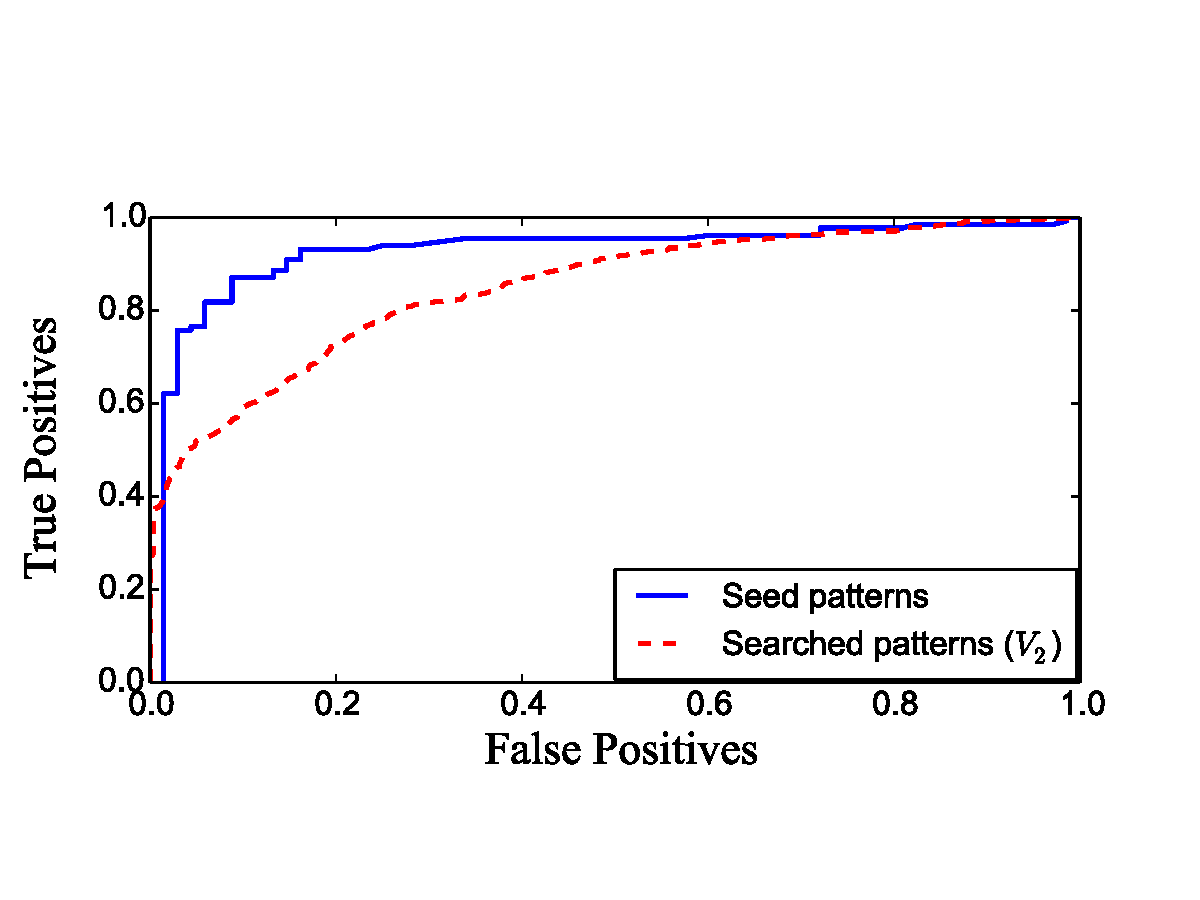
\includegraphics[width=\figSizeEightyFive]{ch06_patterns/figures/discovery/seedROC.pdf}
	\end{center}
	\caption[ROC curve for seed pairs and search patterns]{ROC curve for seed pairs and search patterns (using $\RankRefVar_2$) in the evaluation set.\TODO{This figure uses symbol, check if it matches the text}}%\vspace{-1em}
	\label{fig:combinedROCPatternDiscovery}
\end{figure}


\begin{table} 
	\begin{centering}	
		\begin{tabular}{ c | c c c c}
			\tabletop
			Seed Category   & $\RankRefVar_1$		&	$\RankRefVar_2$ & $\RankRefVar_3$	 &	$\RankRefVar_4$ 	\\	
			\tablemid
			$\seedPattCat_1$ & 0.92    &	0.92		&	0.91    &	0.89\\
			$\seedPattCat_2$ & 0.68    &	0.73		&	0.73    &	0.66\\
			$\seedPattCat_3$ & 0.35    &	0.34    &	0.35    &	0.35\\
			\tablebot
		\end{tabular}
		\caption[\acrshort{map} scores for four variants of rank refinement method for each seed pattern category]{\acrshort{map} scores for four variants of rank refinement method ($\RankRefVar_i$) for each seed category ($\seedPattCat_1$, $\seedPattCat_2$ and $\seedPattCat_3$).}
		\label{tab:meanAveragePrecision_pattern_discovery}
		\par \end{centering}	
\end{table}

\begin{figure}
	\begin{center}
		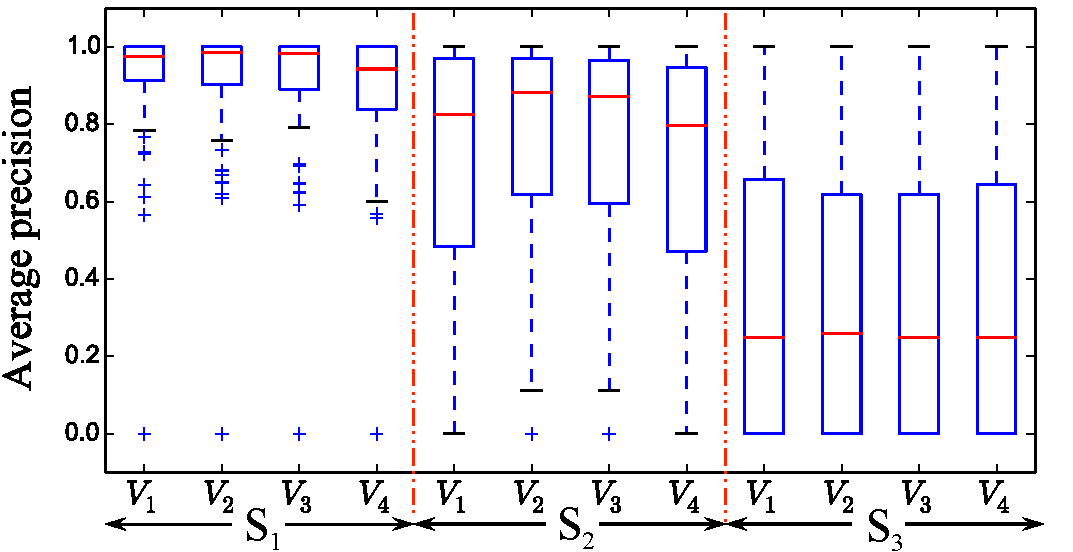
\includegraphics[width=\figSizeEightyFive]{ch06_patterns/figures/discovery/boxPlot.pdf}
	\end{center}
	\caption[Boxplot of average precision values for the different variants of the rank refinement method]{Boxplot of average precision values for the different variants of the rank refinement method ($\RankRefVar_i$) for each seed category.\TODO{This figure uses symbol, check if it matches the text}}
	\label{fig:boxPlotMAPPatternDiscovery}
\end{figure}

Next, we evaluate the performance of inter-recording pattern detection task and assess the effect of the four \gls{dtw} cost variants explained in~\secref{sec:patterns_discovery_results} (denoted by $\RankRefVar_1 \dots \RankRefVar_4$). To investigate the dependence of the performance on the category of the seed pair, we perform the evaluation within each seed category. In~\tabref{tab:meanAveragePrecision_pattern_discovery} we show the \gls{map} scores obtained for the different variants of the rank refinement method ($\RankRefVar_1, \RankRefVar_2, \RankRefVar_3$ and $\RankRefVar_4$) for each seed category ($\seedPattCat_1$, $\seedPattCat_2$ and $\seedPattCat_3$). In addition, we also present a box plot of corresponding average precision values in~\figref{fig:boxPlotMAPPatternDiscovery}. In general, we observe that every method performs well for category $\seedPattCat_1$, with a \gls{map} score around 0.9 and no statistically significant difference between each other. For category $\seedPattCat_2$, $\RankRefVar_2$ and $\RankRefVar_3$ perform better than the rest and the difference is found to be statistically significant. The performance is poor for the third category $\seedPattCat_3$ for every variant. The difference in performance between any two methods across seed categories is statistically significant. We observe that \gls{map} scores across different seed categories correlate strongly with the fraction of melodically similar seed pairs in that category (discussed above). This means that the seed pattern pairs that have high distance $\distPatt$ between them obtain low average precision when used as query patterns and vice-versa. This might be because across repetitions of such patterns there could be a high degree of melodic variation, to model which the current similarity measure appears inadequate. In addition, closely repeating seed pattern pairs (i.e.~with low distance $\distPatt$ between them) might have more number of repetitions with low degree of melodic variations, for which the current similarity measure performs well. 

%It suggests that repeating patterns do have some significance, they are not a product of coincidence, and therefore, they are more likely to recur across recordings. Note that we do not imply that every repeating pattern is (equally) musically significant or is a characteristic phrase of a \gls{raga}. There are different types of repeating patterns in melodies of \gls{iam}. The task of characterizing the discovered patterns is addressed in~\secref{sec:patterns_characterization_of_melodic_patterns} \TODO{rehphrase this last part}
\begin{figure}
	\begin{center}
		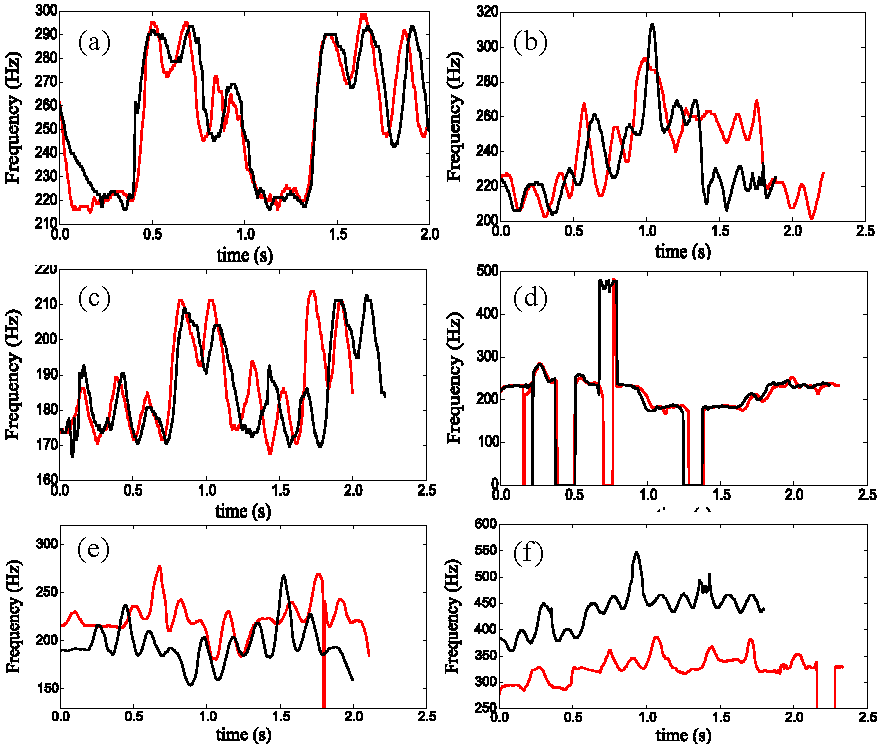
\includegraphics[width=\figSizeHundred]{ch06_patterns/figures/discovery/combinedPatterns.pdf}
	\end{center}
	\caption{Examples of the discovered melodic patterns.\TODO{make the annotations small in size}}
	\label{fig:combinedPatternsDiscovered}
\end{figure}

Finally, we analyze the distance distributions of melodically similar and dissimilar search patterns. For this we use the best performing rank-refinement variant $\RankRefVar_2$. To examine the separation in the distance distribution, we compute the ROC curve as shown in~\ref{fig:combinedROCPatternDiscovery} (dashed red line). We observe that the separability between melodically similar and dissimilar subsequences in this case is poorer than the one obtained for the seed pairs (solid blue line). This suggests that it is much harder to differentiate melodically similar from dissimilar patterns when the search is performed across recordings. This can be attributed to the total number of melodically dissimilar subsequences (irrelevant documents) for every query subsequence, which is orders of magnitude higher in this task compared to the task of pattern discovery within a recording. In addition, one of the reasons can also be that the melodic phrases of two allied \glspl{raga} (\secref{sec:melody_in_iam}) are differentiated based on subtle melodic nuances~\citep{Viswanathan2004}. Hence, one faces a much more difficult task, which requires a superior melodic similarity measure.% Moreover, some of these melodic nuances might be specific to \glspl{raga}, learning which might be possible only under a supervised framework. 

To demonstrate the capabilities of the approach, we show a few examples of the discovered melodic patterns in~\figref{fig:combinedPatternsDiscovered}. Our approach robustly extracts patterns in different scenarios such as large local time warpings~(b), uniform scaling~(c), patterns with silence regions~(d) and across different tonic pitches~(e and f). It is worth mentioning that, during the process of annotation, the musician found several musically interesting results. For example, striking similarity between phrases of two different \glspl{raga}, between phrases in sung melodies and the melodies played on instruments (Violin or \Gls{vina}), and phrases sung by different artists. Many of the discovered patterns are the characteristic melodic phrases of the \glspl{raga}, which are the primary cues for \gls{raga} recognition. All the discovered melodic patterns in this study can be browsed at: \url{http://dunya.compmusic.upf.edu/motifdiscovery/}.  Overall, we find that the obtained results are musically relevant and can be used to establish meaningful relationships between audio recordings. We explore the usability of these discovered patterns in the task of automatic \gls{raga} recognition in~\chapref{chap:raga_recognition}.



%################################################################################################################
%########################################### IMPROVING MELODIC SIMILARITY #######################################
%################################################################################################################


\section{Characterization of Melodic Patterns}
\label{sec:patterns_characterization_of_melodic_patterns}

In the previous section we described our approach to discover melodic patterns in sizable audio music collections of \gls{iam}. Our primary goal was to extract as many different types of repeating melodic patterns and as many occurrences of them as possible, irrespective of their musical relevance\footnote{Note that in our method in~\secref{sec:patterns_melodic_pattern_discovery}, we only removed melodically trivial patterns that comprise primarily single \gls{svara}.}. A well known problem with the computational approaches for musical pattern discovery is the large volume of discovered patterns, wherein a large fraction of them often tends to be musically uninteresting and irrelevant (\secref{sec:pattern_processin_in_music}). This aspect of automated methods for motivic analysis is studied by~\cite{marsden2012counselling}, who says:

\blockquote{\textit{...computational approaches find many more motives and many more relationships between fragments than in traditional motivic analysis...these are then filtered by some mechanism which selects motives and relationships with privileged positions within the network of relationships.}}

Thus, one of the main challenges of pattern discovery methods is to identify the musically meaningful patterns in the output. In the case of melodies in \gls{iam} as well recurring patterns differ drastically in terms of their musical relevance (\secref{sec:melody_in_iam}). Their functional role in melodies varies from being a melodic ornamentation to being a characteristic melodic phrase of a \gls{raga}. Thus, in order to effectively utilize the discovered melodic patterns in different melodic analyses and applications in \gls{iam}, characterization of these patterns in terms of their musical relevance and functional roles is crucial. In this section we address this issue and characterize discovered melodic patterns in order to identify one of the most interesting types of melodic patterns in \gls{iam}, the \gls{raga} motifs.
 
From the literature we see that most of the motivic analysis approaches employ a filtering step to select the musically significant patterns (\secref{sec:motif_in_symbolic_music}). A common approach is to prefer long duration patterns~\citep{Cambouropoulos2006,Karydis2006}. Another type of approaches prefer patterns that occur more frequently than others~\citep{Cambouropoulos2006,meredith2002algorithms}. The methods proposed by~\cite{conklin2010discovery,Conklin2010a} are also based on patterns' frequency of occurrence, but inversely weighted by its frequency of occurrence in an anti-corpus. \cite{collins2011modeling} evaluate several strategies for assigning importance to discovered melodic patterns. A more detailed description of these filtering strategies is provided in~{\secref{sec:motif_in_symbolic_music}. We note that most of these filtering strategies are not directly applicable in our context. For example, since our discovery method operates with a limitation of a fixed length melodic pattern, the strategy of maximal length patterns is not applicable. The other type of commonly used strategy in which the most frequently occurring patterns are selected also appears futile. This is because in \gls{iam} \glspl{gamaka} and several other melodic ornaments are often the most frequently occurring patterns, which in our task are relatively less musically relevant compared to the \gls{raga} motifs. Thus, there is a need for a novel filtering strategy that can characterize discovered melodic patterns in \gls{iam} and can identify the musically interesting ones such as \gls{raga} motifs.	

There is another challenge in dealing with an in-exact or approximate melodic pattern matching methodologies, which is that of determining a meaningful similarity threshold. It becomes an even bigger challenge in an unsupervised analysis, such as the case in our pattern discovery method. The discovery approach described in~\secref{sec:patterns_melodic_pattern_discovery} works with a fixed number of closest pattern matches irrespective of the absolute value of the melodic similarity. As a result of which the output of the pattern discovery approach may contain a large amount of music irrelevant or noisy matches. Although, as seen in~\secref{sec:patterns_discovery_results}, separation between the distance distributions of melodically similar an dissimilar patterns appears favorable (\figref{fig:combinedROCPatternDiscovery}), indicating that an optimal melodic similarity threshold can potentially remove the noisy matches with a reasonable accuracy. However, determining such a melodic similarity threshold is non-trivial.

In this section we address both the issues, determining a meaningful melodic similarity threshold, and characterizing discovered melodic patterns by performing a network analysis. We exploit the topological properties of the network to determine a similarity threshold. For characterizing patterns we first detect non-overlapping communities in the network and then characterize the communities by utilizing the related editorial metadata. As described in~\secref{sec:melody_in_iam}, repeating patterns in melodies of \gls{iam} can belong to varied categories. In order to reduce the complexity involved in identification and evaluation of different types of melodic patterns, we focus on \gls{raga} motifs, which is arguably the most advantageous pattern category for computational melodic analyses of \gls{iam}. \Gls{raga} motifs are learned quite explicitly through years of musical training, and they provide a base for artists' to improvise. Due to these reasons \gls{raga} motifs are distinctly recognized by performing musicians. In addition, such melodic patterns are crucial for \gls{raga} based music retrieval systems, automatic \gls{raga} recognition, studying similarities between artists and recordings, and in developing pedagogical tools for \gls{iam}. Due to these factors we choose \gls{raga} motif category of patterns to study the task of characterization of melodic patterns. In summary, our objective is to discover \gls{raga} motifs in audio collections of \gls{iam}.


\subsection{Method}

The block diagram of the proposed approach is shown in~\figref{fig:block_diagram_characterization}. There are two main processing blocks: (a) melodic pattern discovery and (b) pattern characterization. Both these blocks are described at length in the subsequent sections.

\begin{figure}
	\begin{center}
		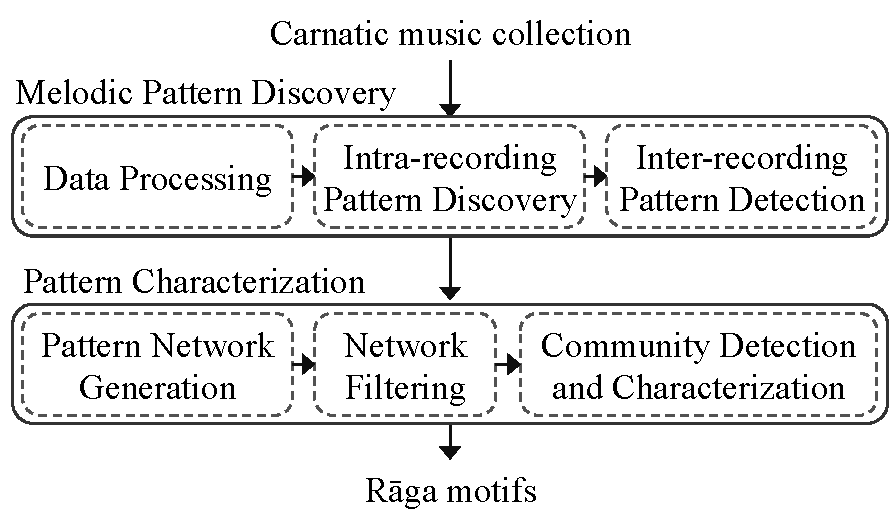
\includegraphics[width=\figSizeSeventy]{ch06_patterns/figures/Characterization/blockDiagram.pdf}
	\end{center}
	\caption[Block diagram for characterizing melodic patterns]{Block diagram of the proposed approach for characterizing melodic patterns.}
	\label{fig:block_diagram_characterization}
\end{figure}


\subsubsection{Melodic Pattern Discovery}
\label{sec:patterns_characterization_pattern_discovery}

As mentioned, discovering melodic patterns in a sizable audio collection of \gls{iam} is a challenging task. To get a reliable input for our approach, we employ the pattern discovery approach we describe in~\secref{sec:patterns_melodic_pattern_discovery}. This is one of the few unsupervised systems, we are aware of, that can discover meaningful melodic patterns in large-scale collections of \gls{iam}. Recall that the output of our pattern discovery approach comprises seed patterns, which are discovered within the recordings, and also, their nearest neighbors in the entire audio collection. In this study, we extract the top 25 closest seed pattern pairs from every recording and consider the top 20 closest patterns for each seed pattern across the recordings. We use the same parameter settings and the implementation of the method as described in~\secref{sec:patterns_melodic_pattern_discovery}. 

Notice that the output of our melodic pattern discovery system may contain a high degree of redundancy in terms of overlapping patterns. This is despite the constraints to only select mutually non-overlapping patterns during the discovery and search phase. This redundancy arises primarily because we perform the inter-recording pattern search for each pattern in the seed pair. Since seed pair patterns are (often) close repetitions of each other, we end up retrieving nearly the same set of patterns as nearest neighbors for both of them. Thus, there exists a large number of overlapping patterns in the output of our pattern discovery block. Despite the known redundancy, we chose to perform inter-recording pattern search for each pattern in the pair separately as it exploits intra-class variability present in the patterns, which might provide better retrieval results.

We reduce the above mentioned redundancy in the output of pattern discovery by following a simple procedure. For every discovered melodic pattern we search for its closest pattern across all the recordings using the same similarity measure as used in the intra-recording pattern discovery block. For each recording we parse a list of patterns in that recording sorted in the increasing order of their distances from their closest patterns. While parsing the list we remove every pattern for which there exists an overlap with another pattern placed higher (lower index) in the sorted list. Thus, at the end of this process we retain only non-overlapping patterns in every recording.



\subsubsection{Melodic Pattern Characterization}
\label{pattern_characterization}

Before we formally describe this processing step, we provide the underlying intuition behind it. As explained earlier, a repeating melodic pattern in \gls{iam} can correspond to either a \gls{raga} motif, a composition-specific motif or to a \gls{gamaka} pattern (\secref{sec:melody_in_iam}). Our objective is to characterize the discovered patterns in order to identify the ones that are \gls{raga} motifs. The information available to accomplish this task is; a bunch of melodic patterns, pitch sequences corresponding to the patterns, editorial metadata of the recordings to which the patterns belongs and the location of the patterns in the recordings. If we take a single melodic pattern, the only possible indicator of its category could be the characteristics of its pitch sequence. However, to the best of our knowledge (acquired from published studies and discussions with musicians), \gls{raga} motifs do not possess any distinctive pitch characteristics. Therefore, characterization of the discovered melodic patterns considering one pattern at a time under unsupervised scenario appears to be virtually impractical. Such melodic motifs are explicitly learned for each \gls{raga} though years of musical training. Despite the importance, a comprehensive published collection of \gls{raga} motifs (audio or pitch sequence) is unavailable. 

Instead of analyzing melodic patterns individually, if we analyze them in clusters, where a cluster comprises melodically similar melodic patterns, we can infer to an extent the categories of these melodic patterns. Consider that we have a cluster of melodic patterns and each pattern comes from a different recording in different \gls{raga}. There is a very high chance that the patterns in the cluster belongs to \gls{gamaka} category, since those patterns occur across \glspl{raga} and across recordings. On the other hand if patterns within a cluster belongs to only one \gls{raga} and different recordings, it is highly likely that the patterns correspond to a \gls{raga} motif. Thus, by analyzing the properties of a cluster in terms of its relation with different musical attributes and editorial metadata, we can characterize the patterns as belonging to \gls{raga} motifs or not. Notice that we eventually exploit the functional roles of different kinds of patterns in melodies of \gls{iam} in order to identify them in a pool of discovered patterns. 

We described above our intuition behind analyzing melodic patterns in units of clusters in order to characterize them. However, clustering melodic patterns further involves many challenges. During clustering we seek to group melodic patterns such that a cluster contains different occurrences of only one melodic phrase. To achieve this, our system should be able to differentiate between melodically similar and dissimilar patterns, for which we need a meaningful similarity threshold. Recall that the extraction of melodic patterns from audio recordings does not involve any similarity thresholding (\secref{sec:patterns_melodic_pattern_discovery}), we select the top 25 and 20 nearest neighbors in discovery and search phase. Determining a musically meaningful similarity threshold in an unsupervised setup is a challenging task, which we address using the concepts of complex networks. 
 
We now formally describe the processing block. As explained, in this block, we aim to first cluster the discovered patterns and then characterize the clusters in order to identify the ones that represent different \gls{raga} motifs. For this, we perform a network analysis in which nodes represent the discovered melodic patterns and edges represent the melodic similarities between these patterns. We described below the processes involved in this task~(\figref{fig:block_diagram_characterization}). 


\paragraph{Pattern Network Generation}
\label{sec:network_generation}

We start by building an undirected weighted network using the discovered melodic patterns from the previous step. The patterns are considered as the nodes of the network and the edge between any two patterns ($i$, $j$) is weighted based on the distance $\distPatt_{ij}$ between the patterns. Noticeably, $\distPatt_{ij}$ is computed using the same distance measure as used in the intra-recording pattern discovery block in~\secref{sec:intraRecordingPatternDiscovery}. The weight of the edge $\edgeWght_{ij}$ between the nodes $i$ and $j$ is given by \eqref{eq:edge_weight_in_network}. 

\begin{equation}
\edgeWght_{ij} = e^{\nicefrac{-\distPatt_{ij}}{\bar{\distPatt}}},
\label{eq:edge_weight_in_network}
\end{equation}

\noindent where, $\bar{\distPatt}$ is the mean of $\distPatt_{ij}$ over every combination of $i$ and $j$. 


\paragraph{Network Filtering}
\label{sec:network_filtering}

The main objective of this processing block is to filter the network in order to retain only the musically meaningful connections between the nodes. Since the edge weights between the pairs of melodically similar and dissimilar nodes may vary by orders of magnitude, we first consider to exploit this heterogeneity to extract the network's backbone. We therefore apply disparity filtering~\citep{Serrano09PNAS} to preserve only the edges that represent statistically significant deviations with respect to a null model of edge weight assignment for every node. The only parameter used in the disparity filtering is the statistical confidence value. We iterate over 5 different confidence values $\lbrace$99.99, 99, 90, 80, 50$\rbrace$. However, as we will show, the application of disparity filtering is found to be quite irrelevant for the present case.

\begin{figure}
	\begin{center}
		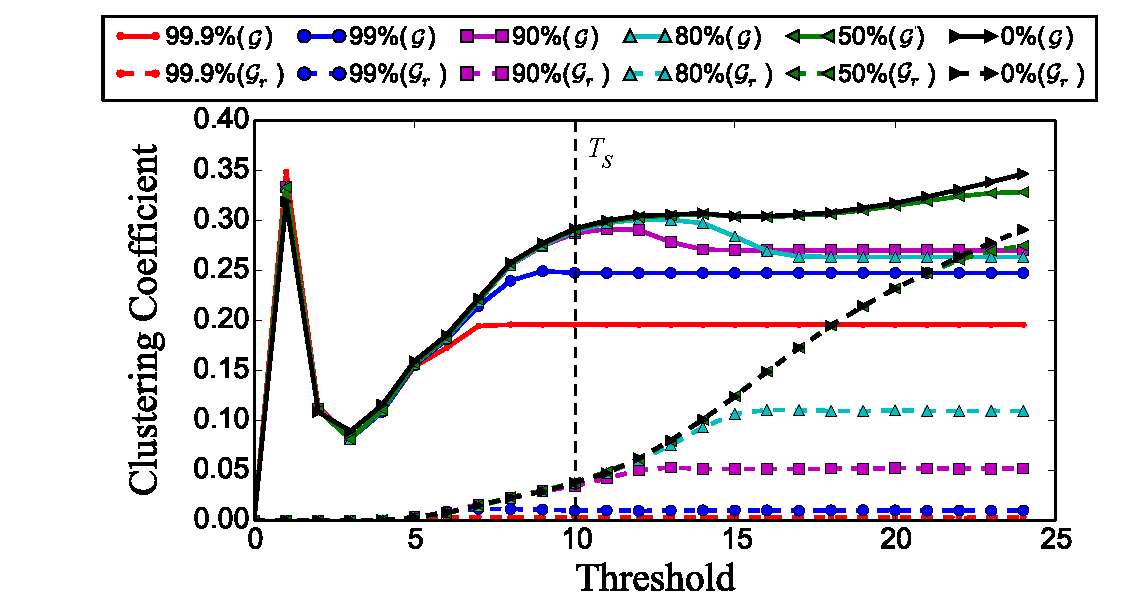
\includegraphics[width=\figSizeEightyFive]{ch06_patterns/figures/Characterization/CC_Curves_shrunk.pdf}
	\end{center}
	\caption[Evolution of clustering coefficient of a network of melodic patterns]{Evolution of the clustering coefficient of $\netUndirWght$ and $\netUndirWght_r$ over different thresholds and for different statistical confidence values used for disparity filtering (legend).\TODO{This figure uses symbol, check if it matches the text}}
	\label{fig:cc_curve_pattern_characterization}
\end{figure}

We next proceed to filter edges in the network based on a melodic similarity threshold $\simThsld$. As mentioned, determining a meaningful similarity threshold in an unsupervised setup is a challenging task. We propose to estimate $\simThsld$ based on the topological properties of the network. For this, we analyze the evolution of the clustering coefficient of both the obtained network $\netUndirWght$ and the corresponding randomized network $\netUndirWght_r$ over a range of similarity thresholds. Clustering coefficient measures the extent to which the nodes in a network tend to cluster together~\citep{newman2003structure}. The randomized network $\netUndirWght_r$ is obtained by swapping the edges between randomly selected node pairs such that the degree of each node is preserved~\citep{maslov2002specificity}. This way, $\netUndirWght_r$ can be considered as the maximally random network with that particular degree distribution. In~\figref{fig:cc_curve_pattern_characterization}, we show the evolution of the clustering coefficient of $\netUndirWght$ and $\netUndirWght_r$ over different similarity thresholds (indicated by exponentially spaced bins). In addition, we can also see the clustering coefficient curves for different statistical confidence values used for disparity filtering. The evolution of the clustering coefficients is used for obtaining a similarity threshold as explained below.

We hypothesize that the more musically meaningful $\simThsld$ is, the higher is the difference between the clustering coefficients of $\netUndirWght$ and $\netUndirWght_r$. We therefore select $\simThsld=10$. Note that even though the similarity threshold corresponding to $\simThsld=1$ results in a higher value of the clustering coefficient, we reject it because the filtered network consists only of a small number of nodes. These nodes correspond to near-exact pattern repetitions discovered within the same recording. Such patterns typically represent composition-specific motifs, and hence are irrelevant in our context. In~\figref{fig:cc_curve_pattern_characterization}, we also observe that the disparity filtering using a confidence value higher than 80\% significantly lowers the clustering coefficient, which can be attributed to the removal of musically meaningful edges in the network. On the other hand, given $\simThsld=10$, the disparity filtering with a confidence value lower than 80\% does not significantly affect the clustering coefficient. We can thus conclude that, in the given scenario, disparity filtering does not bring in any clear advantage. Finally, after applying $\simThsld$, we transform $\netUndirWght$ to an unweighted network. 


\paragraph{Community Detection and Characterization}
\label{sec:patterns_characterization_community_detection}

We next take the unweighted undirected network that results from the previous step, and perform a non-overlapping community detection using the method proposed in~\cite{blondel2008fast}. This method is based on modularity optimization and is parameter-free from the point of view of the user. It has been extensively used in various applications~\citep{fortunato2010community} and can deal with very large networks~\citep{blondel2008fast}. We use the implementation available in networkX~\citep{hagberg-2008-exploring}, a Python language package for exploration and analysis of networks and network algorithms. Using this method for our entire dataset, we obtain around 1800 communities of melodic patterns. 


\begin{figure}
	\begin{center}
		\includegraphics[width=\figSizeHundred]{ch06_patterns/figures/Characterization/networkWithClusters.pdf}
	\end{center}
 \caption[Graphical representation of a network of melodic patterns]{Graphical representation of the melodic pattern network after filtering by threshold $\simThsld$. The detected communities in the network are indicated by different colors. Few examples of these communities are shown on the right.}
 \label{fig:network_and_communities_pattern_characterization}
\end{figure}

To get a better understanding of the network obtained after filtering and the detected communities, we show a graphical representation of the network in~\figref{fig:network_and_communities_pattern_characterization}. We find that many communities comprising large number of nodes in the network correspond to Kampita melodic pattern, which is a kind of \gls{gamaka} that occur in several \glspl{raga} across compositions and hence have large number of occurrences. We also find that the communities with a relatively smaller number of nodes, which in~\figref{fig:network_and_communities_pattern_characterization} appear as isolated communities around the periphery often correspond to the \gls{raga} motifs. A few examples of such communities are shown in~\figref{fig:network_and_communities_pattern_characterization} on the right.

We here define the notation used in the subsequent paragraphs for characterizing pattern communities. A community $\community_q$ is comprised of $N$ nodes, and the node count over different \glspl{raga} is given by the ordered list ${{\nodesCommRaga}_q} = (\nodesCommRaga_{q,1}, \nodesCommRaga_{q,2},\dots$ $\nodesCommRaga_{q,\totalRagasComm})$ such that $\nodesCommRaga_{q,i} \geq \nodesCommRaga_{q,j}$, $\forall~ i < j$,
where each element in $\nodesCommRaga_{q}$ denotes the number of nodes in a particular \gls{raga} and $\totalRagasComm$ is the total number of unique \glspl{raga} comprising the community. Similarly, the node count over the audio recordings is given by the ordered list ${{\nodesCommRec}_q} = (\nodesCommRec_{q,1}, \nodesCommRec_{q,2},\cdots,\nodesCommRec_{q,\totalRecsComm})$ such that $\nodesCommRec_{q,l} \geq \nodesCommRec_{q,m}, \forall~l < m$,  where each element in $\nodesCommRec_{q}$ denotes the number of nodes belonging a particular audio recording and $\totalRecsComm$ is the total number of recordings comprising the community. For both these cases, $\sum_{i=1}^{\totalRagasComm}\nodesCommRaga_{q,i} = \sum_{l=1}^{\totalRecsComm}\nodesCommRec_{q,l} = N$.

We now proceed to characterize the detected communities in order to identify the ones that represent \gls{raga} motifs. For that we first categorize a community $C_q$ as belonging to the \gls{raga} $\RagaOfComm_q$ corresponding to the maximum number of nodes $\nodesCommRaga_{q,1}$ in that community. Subsequently, for each \gls{raga}, we rank all the communities belonging to that \gls{raga}. To rank the communities we empirically devise a goodness measure $\goodnessComm$, which denotes the likelihood that a community $C_q$ represents a \gls{raga} motif. We propose to use

\begin{equation}
\goodnessComm = N \ragaLikelihood^4 \recDistCentroid,
\label{eq:gamma_pattern_characterization}
\end{equation}

where $\ragaLikelihood$ is an estimate of the likelihood of \gls{raga} $\RagaOfComm_q$ in $C_q$, 

\begin{equation}
\ragaLikelihood = \frac{\nodesCommRaga_{q,1}}{N},
\end{equation}

and $\recDistCentroid$ indicates how uniformly the nodes of the community are distributed over audio recordings,

\begin{equation}
\recDistCentroid = \frac{\sum_{l=1}^{\totalRecsComm}l \cdot \nodesCommRec_{q,l}}{N}.
\end{equation}

Higher $\recDistCentroid$ implies a more uniform distribution. Since a community that represents a \gls{raga} motif is expected to contain nodes from a single \gls{raga} (high value of $\ragaLikelihood$) and the nodes belong to many different recordings (high value of $\recDistCentroid$), the goodness measure $\goodnessComm$ is high for such a community. In general we prefer large communities, but, to avoid detecting large communities (high value of N) corresponding to \gls{gamaka} motifs (low value of $\ragaLikelihood$) we use a fourth power on $\ragaLikelihood$. Composition-specific motifs are expected to have a low $\recDistCentroid$, as they are not repeated across multiple recordings, assuming that different recordings correspond to different compositions. 

Note that it might be possible that a music collection contains multiple recordings of the same composition. In such cases, differentiating composition-specific motifs and \gls{raga} motif becomes difficult using $\goodnessComm$ measure. This issue can be overcome with only a trivial modification in our approach, i.e.,~by considering the node distribution ${{\nodesCommRec}_q}$ over compositions instead of recordings. In our current system this could not be implemented because for a number of recordings composition information was unavailable.



\subsection{Evaluation}
\label{sec:patterns_characterization_evaluation}

\subsubsection{Music Collection}
\label{sec:patterns_characterization_music_collection}

The music collection used in this study is a subset of the CompMusic Carnatic music corpus (\secref{sec:corpus_carnatic_music_corpus}). The collection comprises 44 hours of polyphonic audio music recordings of Carnatic music across 10 different \glspl{raga}. For each \gls{raga} we select 16 music pieces, which amounts to a total of 160 recordings. There are 139 vocal music recordings and 21 instrumental recordings comprising violin, \gls{vina} and bamboo flute. In~\tabref{tab:dataset_details_pattern_characterization}, we summarize the relevant details of the dataset. We see that it is diverse in terms of the number of unique compositions and number of lead artists. Furthermore, it includes different forms of compositions (\gls{kirtana}, varnam and viruttam) and recordings containing varied improvised sections such as \gls{alapna}, nereval and kalpan\={a}-\glspl{svara}. %The \glspl{raga} selected here are amongst the most frequently performed \glspl{raga} in the CompMusic Carnatic music corpus, which in turn is representative of the Carnatic music repertoire~\cite{CM_Corpora_Ajay14}. 
The chosen \glspl{raga} contain diverse set of \glspl{svara} (notes) both in terms of the number of \glspl{svara} and their pitch classes (svarasth\={a}n\={a}s). From~\tabref{tab:dataset_details_pattern_characterization}, 
we also notice that several \glspl{raga} such as Kaly\={a}\d{n}i, K\={a}mb\={o}ji and B\={e}gada have a large fraction of \glspl{svara} in common. We refer to them as allied \glspl{raga} (\secref{sec:melody_in_iam}). This further increases the complexity of the task at hand, since the discrimination between the phrases of allied \glspl{raga} may be based on subtle melodic nuances.

\COMMENT{availability of the dataset?}

\begin{table} 
	%\tabcolsep = 0.1cm
	\centering
	\begin{tabular}{ l  | c c c c}
\tabletop
		\Gls{raga}   		& 	Dur 	&	\#Com		&	\#Art	&	Svaras\\	
\tablemid
		Hamsadhvani 		& 	2.46 		&	12			&	14		&	$s\,r_2\,g_3\,p\,n_3$\\
		K\={a}mavardhini 	& 	3.94 		&	13			&	16		&	$s\,r_1\,g_3\,m_2\,p\,d_1\,n_3$\\		
		Darb\={a}r   		& 	2.59 		&	8			&	13		&	$s\,r_2\,g_2\,m_1\,p\,d_2\,n_2$\\	
		Kaly\={a}\d{n}i   	& 	6.94 		&	9			&	16		&	$s\,r_2\,g_3\,m_2\,p\,d_2\,n_3$\\	
		K\={a}mb\={o}ji   	& 	6.91 		&	12			&	13		&	$s\,r_2\,g_3\,m_1\,p\,d_2\,n_2\,n_3$\\	
		B\={e}ga\d{d}a   	& 	3.41 		&	9			&	16		&	$s\,r_2\,g_3\,m_1\,p\,d_2\,n_2\,n_3$\\	
		K\={a}pi   			& 	2.24 		&	12			&	16		&	$s\,r_2\,g_2\,g_3\,m_1\,p\,d_2\,n_2\,n_3$\\	
		Bhairavi   			& 	5.33 		&	7			&	16		&	$s\,r_2\,g_2\,m_1\,p\,d_2\,d_3\,n_2$\\	
		Beh\={a}g   		& 	1.51 		&	12			&	16		&	$s\,r_2\,g_3\,m_1\,m_2\,p\,d_2\,n_2\,n_3$\\	
		
		T\={o}\d{d}i   		& 	8.75 		&	12			&	16		&	$s\,r_1\,g_2\,m_1\,p\,d_1\,n_2$\\	
\tablebot
		Total 	& 	44.08 		&	106			&	57		&	-\\	
\tablebot
	\end{tabular}
	\caption[Details of the dataset used for studying pattern characterization]{Details of the dataset in terms of the duration (Dur) in hours, number of unique compositions (\#Com), unique lead artists (\#Art), and the svaras for each \gls{raga}. Here $s,r,$ $g,m,p,d,n$ denote the 7 svaras in IAM and the subscript indicates the variant of the svar for a particular \gls{raga} (cf.~\citep{Viswanathan2004}).}
	\label{tab:dataset_details_pattern_characterization}
\end{table}

\subsubsection{Setup and Evaluation Measures}
\label{sec:patterns_characterization_experimental_setup}

Given the unsupervised nature of this study, we perform a listening test to formally evaluate the extent to which the selected melodic phrases correspond to \gls{raga} motifs. For each of the 10 \glspl{raga} in the dataset, we select the top 10 communities based on the goodness measure $\goodnessComm$ (\eqnref{eq:gamma_pattern_characterization}). From each of these communities, we select their representative melodic phrase based on the betweenness centrality of the nodes~\citep{newman2003structure}, i.e.,~the node with the highest betweenness centrality is considered as the representative melodic phrase of that community. In case of a tie, we select the one with the highest node degree~\citep{newman2003structure}. Finally, we  arrive at a set of 100 melodic phrases, which are then used to perform the listening test. These audio examples are also made available online\footnote{http://compmusic.upf.edu/node/277}.

For the listening test we select 10 professional Carnatic musicians with over 15 years of formal music training. Each musician is presented with the audio fragments corresponding to the selected melodic phrases in a random order. They are also presented with the \glspl{raga} corresponding to the melodic phrases. The musicians are asked to rate each melodic phrase based on whether it is a characteristic phrase of that \gls{raga}. We use binary ratings (`Yes' or `No'). 

The audio fragments were segmented with a one second buffer on either side of the phrase to offer some context and reduce the effect of abrupt boundaries. % Thus, a 4\,s audio fragment was presented to the musicians.  
In order to quantify the musicians' assessment, we use mean ratings for each phrase $\pattern$, $\mu_\pattern$, considering `Yes' as 1 and `No' as 0. For analyzing the ratings per \gls{raga}, we study the mean and standard deviation of all $\mu_\pattern$ for phrases in every \gls{raga}, which we denote by $\mu_\recording$ and $\sigma_\recording$, respectively.


\subsection{Results and Discussion}
\label{sec:patterns_characterization_results_and_discussion}

We first analyze the musicians' ratings at the level of melodic phrases. In~\figref{fig:average_rating_pattern_characterization}, we show $\mu_\pattern$ for the 100 selected melodic phrases, where the grouping is based on their corresponding \glspl{raga}. We find that the mean and the standard deviation of $\mu_\pattern$ for the melodic phrases is 0.85 and 0.16, respectively. For a better understanding of $\mu_\pattern$ across phrases and the overall musicians' agreement, we show the histogram of $\mu_\pattern$ in~\figref{fig:average_rating_histogram_pattern_characterization}. We see that 33 melodic phrases are rated as \gls{raga} motifs by all 10 musicians and 25 phrases are rated as \gls{raga} motifs by 9 out of 10 musicians. Similarly, the musicians' agreement can be inferred for the rest of the phrases from this histogram. We observe that 91\% of the phrases are always marked as \gls{raga} motifs by at least 7 out of 10 musicians. 


\begin{figure}
	\begin{center}
		\includegraphics[width=\figSizeSixty]{ch06_patterns/figures/Characterization/per_raaga_per_phrase_rating.pdf}
	\end{center}
	\caption[Mean musician ratings for the discovered melodic phrases]{Mean musician rating per melodic phrase for each \gls{raga}: K\={a}pi\,(Kp), Hamsadhvani\,(Hd), K\={a}mavardhini\,(Kv), Bhairavi\,(Bh), Beh\={a}g\,(Bg), T\={o}\d{d}i\,(Td), B\={e}ga\d{d}\={a}\,(Bd), Kaly\={a}\d{n}\={i}\,(Kl), Darb\={a}r\,(Db), K\={a}mb\={o}ji\,(Kb).}
	\label{fig:average_rating_pattern_characterization}
\end{figure}


We now proceed to analyze the results for different \glspl{raga}. In~\tabref{tab:results_per_raaga_pattern_characterization}, we summarize mean $\mu_\recording$ and standard deviation $\sigma_\recording$ of $\mu_\pattern$ for each \gls{raga}. We observe that there is a considerable amount of variation in $\mu_\recording$ across the \glspl{raga}. It ranges from 0.75 for \gls{raga} K\={a}pi to 0.92 in the case of \gls{raga} T\={o}\d{d}i. An interesting observation here is that the phrase-based \glspl{raga}\footnote{R\={a}gas whose identity is derived based on phraseology than svaras~\cite{krishna2012carnatic}.\TODO{put a section ref instead of the footnote}} are the top performing \glspl{raga} with the  exception of \gls{raga} Darb\={a}r. From~\tabref{tab:results_per_raaga_pattern_characterization} and \tabref{tab:dataset_details_pattern_characterization}, we notice a strong correlation between $\mu_\recording$ and the total duration of the audio recordings across \glspl{raga}. This suggests that longer music pieces are likely to facilitate the discovery of \gls{raga} motifs owing to more number of occurrences of such melodic phrases.

We examine the melodic phrases with low scores. An investigation of 9 out of 100 phrases that obtain $\mu_\pattern\leq0.6$ reveals that many of these phrases are composition-specific phrases that do not characterize the \gls{raga}. The method wrongly identifies them as \gls{raga} motifs because their associated communities have a high $\goodnessComm$ score owing to a high $\recDistCentroid$ value. This can be attributed to the fact that these phrases are discovered from multiple recordings, since their corresponding compositions have several recordings in the dataset.  As described in~\secref{sec:patterns_characterization_community_detection}, in such a scenario, the goodness measure $\goodnessComm$ can be made more robust to such cases by computing $\recDistCentroid$ using the distribution of nodes ${{\nodesCommRec}_q}$ over unique compositions rather than over audio recordings.

The results show that the proposed method successfully discovers \gls{raga} motifs with a high accuracy. We see that, even for the allied \glspl{raga} present in the dataset such as K\={a}mb\={o}ji and B\={e}gada (\secref{sec:patterns_characterization_music_collection}), the method is able to discover distinct characteristic \gls{raga} motifs. As mentioned, allied \glspl{raga} are challenging because they have a substantial overlap in the set of svaras that they comprise (see also~\tabref{tab:dataset_details_pattern_characterization}). Finally, on a more informal side, it is worth mentioning that musicians were impressed when, after the listening test, they came to know that the melodic phrases were discovered by a machine following an unsupervised approach. 


\begin{figure}
	\begin{center}
		\includegraphics[width=\figSizeSixty]{ch06_patterns/figures/Characterization/histogram_musician_rating.pdf}
	\end{center}
	\caption[Histogram of mean musician ratings for 100 melodic phrases]{Histogram of $\mu_\pattern$ for all 100 melodic phrases selected for the listening test.}
	\label{fig:average_rating_histogram_pattern_characterization}
\end{figure}


\begin{table} 
	%\tabcolsep = 0.1cm
	\centering
	\begin{tabular}{ l  c c| l | c c }
		\hline\hline
		\multicolumn{1}{ l|  }{\Gls{raga}}   			& 	$\mu_\recording$ 	&	$\sigma_\recording$	& \Gls{raga}   			& 	$\mu_\recording$ 	&	$\sigma_\recording$\\	
		\hline
		\multicolumn{1}{ l|  }{Hamsadhvani} 			& 	0.84 		&	0.23 & {\bf B\={e}ga\d{d}a}   	& 	0.88 		&	0.11	\\
		\multicolumn{1}{ l|  }{K\={a}mavardhini} 	& 	0.78 		&	0.17 & K\={a}pi   			& 	0.75 		&	0.10\\	
		\multicolumn{1}{ l|  }{Darb\={a}r}   		& 	0.81 		&	0.23 & {\bf Bhairavi}   			& 	0.91 		&	0.15\\	
		\multicolumn{1}{ l|  }{\bf Kaly\={a}\d{n}i}  & 	0.90 		&	0.10 & Beh\={a}g   		& 	0.84 		&	0.16\\	
		\multicolumn{1}{ l|  }{\bf K\={a}mb\={o}ji}   	& 	0.87 	&	0.12 & {\bf T\={o}\d{d}i}   		& 	0.92 		&	0.07\\	
		\hline\hline
		%   			& 				& 		& 	Overall&0.85 		&	0.16\\ \cline{4-6}\cline{4-6}
		%\hline\hline 
	\end{tabular}
	\caption[Mean and standard deviation of $\mu_\pattern$ for each \gls{raga}]{Mean ($\mu_\recording$) and standard deviation ($\sigma_\recording$) of $\mu_\pattern$ for each \gls{raga}. R\={a}gas with $\mu_\recording \geq 0.85$ are highlighted. }
	\label{tab:results_per_raaga_pattern_characterization}
\end{table}


We consider this work as a preliminary study with a lot of scope for improvements. In particular, the approach can be extended to identify patterns belonging to other categories (\gls{gamaka} or composition-specific patterns), definition of the goodness measure $\goodnessComm$ can be improved as suggested in~\secref{sec:patterns_characterization_results_and_discussion}, listening test could be done more rigorously by including negative examples (\gls{gamaka} patterns), and the resultant patterns of the approach can be quantitatively evaluated by using them in tasks such as composition identification. On these lines, in~\secref{sec:phrase_based_feature_extraction} we present an approach that uses clustered melodic patterns to perform the task of automatic \gls{raga} recognition. That way, in addition to the qualitative assessment as done in this work, we can also quantitatively assess the musical relevance of the extracted and characterized melodic patterns.



\section{Summary and Conclusions}
\label{sec:conclusions_patterns}

In this chapter we presented our methodology for discovering musically significant melodic patterns in sizable audio music collections of \gls{iam}. Our methods utilize the  melodic representations and descriptors obtained in~\chapref{chap:data_preprocessing}, and combine concepts from music signal processing, time-series analysis, information retrieval, and complex networks to successfully extract musically meaningful melodic patterns in audio collections. We studied three main tasks involved in this process; melodic similarity, pattern discovery, and characterization of the discovered melodic patterns. 

We first carried out an in-depth supervised analysis of melodic similarity, which is a crucial component in pattern discovery. We evaluated 560 different combinations of various computational procedures and parameters values that are often used for this task. We showed that melodic similarity computation is very sensitive to the choice of parameters and processing steps. A higher sampling rate of the melody representation and mean normalization is desired for computing a reliable melodic similarity in Carnatic music. For Hindustani music, on the other hand, sampling rate (within the considered range) has no significant affect on the performance and tonic normalization of the melody results in a better performance. In general, \gls{dtw}-based distance measure performs better than the Euclidean distance, and the usage of local constraint in \gls{dtw} enhances the performance. The \gls{dtw} variant without any global constraint is preferred (specially for Hindustani music), which suggests that there are large non-linear timing variations across occurrences of the melodic pattern. We observed that an accurate segmentation of the melodic patterns has a huge positive impact on the computation of melodic similarity. The best methodology variant thus identified for melodic similarity is further improved by addressing two specific challenges that arise due to large non-linear timing variations and rapid melodic movements in melodic patterns. The solution we proposed exploits specific melodic characteristics that are particular to \gls{iam}. We showed that duration truncation of the steady \gls{svara} regions in melodic phrases results in a statistically significant improvement in the computation of melodic similarity. Furthermore, we showed that the complexity of a melodic pattern in Carnatic music is a distinguishing aspect of the pattern, and can be successfully utilized to improve melodic similarity.

Subsequently, we presented our data-driven unsupervised approach for discovering repeated melodic patterns in large audio collections of \gls{iam}. We first discovered seed patterns within a recording, and later, used those as queries to detect similar occurrences in the entire music collection. We used \gls{dtw}-based distance measures to compute melodic similarity and compared four different rank refinement variants. Discovering 25 closest seed pattern pairs within each recording and retrieving their 200 closest patterns in an audio collection of 365\,hours of Carnatic music comprising 1764 recordings results in around 12 trillion distance computations. We showed that using cascaded lower bounding techniques borrowed from time-series analysis we save nearly 76\% of the total computations for the intra-recording pattern discovery task and around 99\% of the total computations for the inter-recording pattern detection task. Thus, such indexing techniques can scale \gls{dtw} on hundreds of hours of music collections. We evaluated a randomly sampled subset of the extracted melodic patterns comprising 8000 patterns by performing listening tests by a professional Carnatic musician. Our quantitative evaluation based on the expert feedback indicated that a \gls{dtw}-based distance measure performs well for intra-recording discovery. However, the performance for the inter-recording pattern detection task is inferior suggesting that we require better melodic similarity measures for searching occurrences across recordings. Qualitative feedback from the musician suggests that the extracted melodic patterns are interesting and contain several instances of musically significant patterns such as \gls{raga} motifs. 

The output of the pattern discovery method contains different types of repeating patterns. We presented an approach to identify musically significant patterns, the \gls{raga} motifs, and specifically, to distinguish them from \gls{gamaka} and composition-specific patterns (\secref{sec:melody_in_iam}).  We employed a network analysis and  use a non-overlapping community detection algorithm to cluster melodic patterns. Using the topological properties of the network, we determined a musically meaningful similarity threshold. We devised a goodness measure for characterizing the detected communities. In a listening test with 10 professional Carnatic musicians we showed that the proposed method successfully discovers \gls{raga} motifs with accuracy, even in the presence of allied \glspl{raga} in the dataset. Thus, we demonstrated that the methodology we use to determine melodic similarity threshold and to define the goodness measure successfully identifies musically significant patterns.  Our results show that the functional roles of different melodic phrases in \gls{iam} can be effectively exploited to identify them in an unsupervised manner. To the best of our knowledge, utilization of the functional roles of different melodic patterns in \gls{iam} in order to describe and characterize them is done for the first time.

Overall, we  showed that our unsupervised methodology that does not require any exemplar patterns can successfully discover musically significant melodic patterns (\gls{raga} motifs) in sizable music collections of \gls{iam}.  These patterns can be used in a number of \gls{mir} tasks and applications for \gls{iam}. Due to their importance in characterizing \glspl{raga} they can immediately be utilized for automatic \gls{raga} recognition, a topic that we study in~\chapref{chap:raga_recognition}. These patterns can be used to interlink large volumes of audio recordings in order to define novel music similarity measures, and to perform musicologically relevant studies such as characterization of \glspl{raga}, artists, and compositions in \gls{iam}. Furthermore, there can be enhanced listening music applications, and pedagogical tools that can potentially utilize these melodic patterns. Concrete examples of such applications are provided in~\chapref{sec:applicatoins}.


%FUTURE WORK
%
%It would also be worthwhile to explore the applicability of this approach to music traditions such as Flamenco, Beijing opera and Turkish Makam music.
%
% In the future, we plan to improve the method used for segmenting the steady \gls{svara} regions so that it can differentiate melodic ornaments from subtle \gls{svara} transitions. In addition, we see a vast scope in further refining the complexity estimate of a melodic phrase to improve the complexity weighting. 
% using composition info in communities can further boost the performance of our characterization process. 

%\cleartorecto%!TEX root = ../thesis_a4.tex

\chapter{\titlecap{Automatic \glsentrytext{raga} Recognition}}
\label{chap:raga_recognition}


%0) What is automatic raga identification
%1) Motivation and relevance of the problem
%2) References to thousands of papers that cater to this task
%3) What lacks in them
%4) How do we fill in the missing gaps
%5) What we present in this chapter
%6) What are the papers which this chapter is based on


\section{Introduction}

In this chapter we address the task of automatically recognizing \glspl{raga} in audio recordings of \gls{iam}. We describe two novel approaches for \gls{raga} recognition that jointly capture the tonal and the temporal aspects of melody. The contents of this chapter are largely based on our published work in~\cite{gulatiphrase_2016} and in~\cite{gulati_tdms_2016}.

As mentioned before, \gls{raga} is a core musical concept used in the composition, performance, organization, and pedagogy of \gls{iam}. \Gls{raga} of the musical piece is the most desired melodic description of a recorded performance by the listeners. Numerous compositions in Indian folk and film music are also based on \glspl{raga}~\citep{ganti2013bollywood}. Despite its significance in \gls{iam}, there exists a large volume of audio content whose \gls{raga} is incorrectly labeled or, simply, unlabeled. A computational approach to \gls{raga} recognition will allow us to automatically annotate large collections of audio music recordings. It will enable \gls{raga}-based music retrieval in large audio archives, semantically-meaningful music discovery and musicologically-informed navigation. Furthermore, a deeper understanding of the \gls{raga} framework from a computational perspective will pave the way for building applications for music pedagogy in \gls{iam}. 

\Gls{raga} recognition is the most studied research topic in \gls{mir} of \gls{iam}. There exist a considerable number of approaches utilizing different characteristic aspects of \glspl{raga} such as \gls{svara} set, \gls{svara} salience and \gls{arohana}-\gls{avrohana}. A critical in-depth review of the existing approaches for \gls{raga} recognition is presented in \secref{sec:sota_raga_recognition}, wherein we identified several shortcomings in these approaches and different venues for scientific contribution to take this task to the next level. Here we summarize the main areas of improvement that are identified based on our literature review (\secref{sec:sota_raga_recognition}). 

\begin{itemize}
	\item Around half the number of the existing approaches for \gls{raga} recognition do not utilize the temporal aspects of melody at all (\tabref{tab:raga_recognition_methods_melodic_characteristics}), which are crucial in characterizing \glspl{raga}. Approaches that do utilize the temporal aspects, invariably consider a discrete representation of melody in the analysis . Such approaches fall short of capturing the characteristics of the continuous melodic transitions across the \glspl{svara}, which is a relevant information for \gls{raga} recognition. Thus, approaches that can work with a continuous melody representation and still can utilize effectively the temporal aspects of melody are worth exploring for this task.
	
	\item The complexity in the task of recognizing \glspl{raga} is dependent on the number of \glspl{raga} to be differentiated, and the set of \glspl{raga} considered together. Many existing approaches are evaluated with only a few number of \glspl{raga}. Approaches that include considerable number of \glspl{raga} often include only a handful of audio recordings per \gls{raga}. A sizable, diverse and representative dataset of Hindustani and Carnatic music that can be shared and used across studies will be instrumental in systematically improving the state-of-the-art in \gls{raga} recognition.
	
	\item A thorough comparative  evaluation of the existing methods is missing in the literature. Most of the studies only evaluate their proposed method and do not perform any comparison with the existing studies. An exhaustive comparison of different approaches on the same dataset and under the same experimental setup is needed in order to identifying the strengths and weaknesses of these methods.
	
\end{itemize}

\begin{figure}
	\begin{center}
		\includegraphics[width=\figSizeEightyFive]{ch07_ragaRecognition/figures/figure_todo.pdf}
	\end{center}
	\caption{Overall block diagram for automatic \gls{raga} recognition.}
	\label{fig:bd_raga_recognition}
\end{figure}

We address the above mentioned issues in our work. We put a significant amount of effort in compiling and curating sizable datasets for evaluating the task of \gls{raga} recognition for both Hindustani and Carnatic music. To the best of our knowledge these are the largest datasets every used for evaluating \gls{raga} recognition methods. Furthermore, to encourage reproducible research we also make these datasets publicly available online (\appref{app:resources}). 

\XXX{S}{J}{Do you think this following paragraph make sense? I wanted to put both the methods under a common framework, to structure it mentally}
We describe two novel methods for \gls{raga} recognition \acrshort{ragarecVSM} and \acrshort{ragarecTDMS} that overcome a number of shortcomings in the existing approaches as enumerated above and in our literature review (\secref{sec:sota_raga_recognition}). A general block diagram for both the methods is shown in Figure~\ref{fig:bd_raga_recognition}. There are two main processing blocks; feature extraction and classification. Given sets of audio recordings for training ($\mathrm{\corpus}_\mathrm{tr}$) and testing ($\mathrm{\corpus}_\mathrm{ts}$) we first extract features ($\mathrm{F}_\mathrm{tr}$ and $\mathrm{F}_\mathrm{ts}$) for every audio recording in both the sets. Subsequently features of the training set $\mathrm{F}_\mathrm{tr}$ along with the \gls{raga} labels $\mathrm{L}_\mathrm{tr}$ are used to train a classifier to build a classification model. Using this model we then predict the \gls{raga} labels for the testing set $\mathrm{L}_\mathrm{ts}$. \acrshort{ragarecVSM} and \acrshort{ragarecTDMS} differ both in terms of the extracted features and the classification strategy. Both these methods are described at length in the subsequent sections.



\section{\titlecap{Vector Space Modeling for \glsentrytext{raga} Recognition}}
\label{sec:phrase_based_feature_extraction}

In this section, we describe our method (\acrshort{ragarecVSM}) that is based on melodic patterns and employs vector space modeling for \gls{raga} recognition. This method utilizes melodic patterns discovered from audio recordings of \gls{iam} in an unsupervised manner using the approach we described in the previous chapter (\chapref{}). 

As mentioned before, every \gls{raga} has a set of characteristic melodic patterns that capture the essence of the \gls{raga}. These melodic patterns are one of the most prominent cues for \gls{raga} identification, used both by a performer and a listener (\secref{sec:melody_in_iam}). They act as a building block to construct melodies both in composition and improvisation. However, despite the importance of melodic patterns in characterizing \glspl{raga}, they are not fully exploited by the computational methods for \gls{raga} recognition.  There exist only a handful of approaches that utilize melodic patterns for this task (\secref{sec:sota_raga_recognition}). However, they work with a discrete representation, and pre-defined dictionaries of these patterns, thus limiting the potential of a pattern-based approach for \gls{raga} recognition. This can be attributed primarily to the challenges involved in the extraction of musically meaningful melodic patterns from the audio music recordings. To the best of our knowledge there exists only one approach that uses discovered melodic patterns for this task~\citep{shrey_ISMIR_2015}. Although, the authors extract these patterns in specific sections (Pallavi lines) of audio recordings in Carnatic music and address the task of \gls{raga} verification, and not \gls{raga} recognition. A detailed discussion on the existing approaches and their shortcomings is provided in \secref{sec:sota_raga_recognition}.

Before describing our method we first present the intuition and motivation behind the approach. A number of similarities can be seen between a \gls{raga} rendition and a textual description of a topic. Like an author describes a topic by using different relevant words to the topic, an artist renders a \gls{raga} by using appropriate melodic phrases that suit the context. There are words that are quite specific to a topic, which are analogous to the characteristic melodic phrases of a \gls{raga}. Stop words not specific to any topic or to a document can be seen as analogous to the generic \gls{gamaka} type melodic patterns, which are not specific to a \gls{raga} or to a recording (\secref{sec:recurring_melodic_patterns_iam}). Words that are specific to a document can be regarded as composition specific melodic patterns. This analogy drives the proposed method and motivates to employs concepts of \gls{vsm}. The approach in several sense is inspired by the approaches typically used for topic modeling and document classification\COMMENT{Is any ref needed here?}. We now proceed to describe our method in detail.

\COMMENT{if time permits write pros and cons of this approach.}

%Merits and shortcomings of this method are summarized below:
%\begin{itemize}
%	\item Human interpretation of the intermediate output, usability of intermediate outputs, exploiting the most characteristic aspect of a raga. Utilize both the tonal and the pitch information. Exploit characteristic movements between the svaras as well as sequence of svaras
%	\item No need for analyzing whole melody, if patterns are identified in chunks raga can be identified.
%	\item Musically meaningful relatinos between recordings can be established.
%\end{itemize}
%
%Cons
%\begin{itemize}
%	\item Prone to octave errors, not statistical, spurts of error can deprove the performance enormously
%	\item Extraction of characteristic melodic patterns is still a challenging process. Limited by that performance
%	\item Affected a lot by the improvisational aspects
%	\item Computationally challenging. 
%	\item Does not exploit global melodic characteristics.
%\end{itemize}
%

\begin{figure}
	\begin{center}
		\includegraphics[width=\figSizeSeventy]{ch07_ragaRecognition/figures/bd_phasebased_raga_recognition.pdf}
	\end{center}
	\caption{Block diagram of the proposed phrase-based approach to \gls{raga} recognition.}
	\label{fig:bd_phasebased_raga_recognition}
\end{figure}


\subsection{Feature Extraction}
\label{sec:vsm_feature_extraction}

The block diagram for feature extraction in \acrshort{ragarecVSM} is shown in Figure~\ref{fig:bd_phasebased_raga_recognition}. There are three main processing blocks; melodic pattern discovery, melodic pattern clustering and feature extraction. Below we describe each of these blocks in detail. 

\subsubsection{Melodic Pattern Discovery}
\label{sec:vsm_feature_extraction_pattern_discovery}
In this block we extract melodic patterns from the collection of audio recordings. There are three main processing modules in this block; data-processing, intra-recording pattern discovery and inter-recording pattern search. All these modules are same as described already in Section~XXX. We use the same set of parameter settings as mentioned in their description.

\subsubsection{Melodic Pattern Clustering}
\label{sec:vsm_feature_extraction_pattern_clustering}

In this block we cluster the discovered melodic patterns obtained in the previous step. The objective is to group together all the patterns that are different occurrences of the same melodic phrase. For this, we propose to perform a network analysis in which the clustering is performed using a non-overlapping community detection method. 

We start by building an undirected network $\netUndirWght$ using the discovered patterns as the nodes of the network. We connect any two nodes only if the distance between them is below a similarity threshold $\simThsld$. Noticeably, this distance is computed using the same measure as used in the pattern discovery block (Section~XXXX). The weight of the edge, when it exists, is set to 1. Non-connected nodes are removed.

As mentioned before determining a meaningful similarity threshold in an unsupervised manner is a complex task. For estimating an optimal value of $\simThsld$ we follow the approach as described in Section~\TODO{XXX}. We compare the evolution of the clustering coefficient $\clusCoff$ of the obtained network $\netUndirWght$ with a randomized network $\netUndirWght_r$ over different distance thresholds $\simThsld$. The randomized network $\netUndirWght_r$ is obtained by swapping the edges between randomly selected pairs of nodes such that the degree of each node is preserved~\cite{maslov2002specificity}. The optimal threshold $\simThsld^\star$ is taken as the distance that maximizes the difference between the two clustering coefficients.  In Figure~\TODO{XXX}, we show $\clusCoff(\netUndirWght)$, $\clusCoff(\netUndirWght_r)$ and $\clusCoff(\netUndirWght)-\clusCoff(\netUndirWght_r)$ for different values of $\simThsld$, and mark the optimal threshold $\simThsld^\star$.

The next step of our approach (Figure~\ref{fig:bd_phasebased_raga_recognition}) groups similar melodic patterns as done in Section~\TODO{XXX}. To do so, we detect non-overlapping communities in the network of melodic patterns using the method proposed in~\cite{blondel2008fast}. This method is based on optimizing the modularity of the network and is parameter-free from the user's point of view. This method is capable of handling very large networks and has been extensively used in various applications~\cite{fortunato2010community}. We use its implementation available in networkX~\cite{hagberg-2008-exploring}, a Python language package for exploration and analysis of networks and network algorithms. Note that, from now on, the melodic patterns grouped within a community are regarded as the occurrences of a single melodic phrase. Thus, a community essentially represents a melodic phrase or motif.

\subsubsection{TFIDF Feature Extraction}
\label{sec:vsm_feature_extraction_TFID_computation}

As mentioned above, we draw an analogy between r\={a}ga rendition and textual description of a topic. Using this analogy we represent each audio recording using a vector space model. This process is divided into three blocks (Figure~\ref{fig:bd_phasebased_raga_recognition}).

We start by building our vocabulary $\pattVocab$, which translates to selecting relevant communities (melodic phrases) for characterizing r\={a}gas. For this, we include all the detected communities except the ones that comprise patterns extracted from only a single audio recording. Such communities are analogous to the words that only occur within a document and, hence, are irrelevant for modeling a topic. The size of the obtained vocabulary $\pattVocab$ corresponding to the optimal threshold mentioned above ($\simThsld^\star=9$) is XXX.

We experiment with three different sets of features $\featureVSMOne$, $\featureVSMTwo$ and $\featureVSMThree$, which are similar to the term frequency-inverse document frequency features typically used in text information retrieval. We denote our corpus by $\corpus$  comprising $N = |\corpus|$ number of recordings. A melodic phrase and a recording is denoted by $\pattern$ and $\recording$ , respectively

\begin{equation}
\featureVSMOne(\pattern,\recording)= 
\begin{cases}
1				,& \text{if}~~\feaqPhRec(\pattern,\recording) > 0\\
0,              & \text{otherwise}
\end{cases}
\end{equation}
where, $\feaqPhRec(\pattern,\recording)$ denotes the raw frequency of occurrence of phrase $\pattern$ in recording $\recording$. $\featureVSMOne$ only considers the presence or absence of a phrase in a recording. In order to investigate if the frequency of occurrence of melodic phrases is relevant for characterizing r\={a}gas, we take $\featureVSMTwo(\pattern,\recording) = \feaqPhRec(\pattern,\recording)$. As mentioned, the melodic phrases that occur across different r\={a}gas and in several recordings are futile for r\={a}ga recognition. Therefore, to reduce their effect in the feature vector we employ a weighting scheme, similar to the inverse document frequency ($\mathrm{idf}$) weighting in text retrieval.
\begin{equation}
\featureVSMThree(\pattern,\recording) = \feaqPhRec(\pattern,\recording) \times \irf(\pattern,\corpus)
\end{equation}
\begin{equation}
\irf(\pattern,\corpus) = \log \left( \frac{N}{ |\lbrace \recording \in \corpus: \pattern \in \recording \rbrace|} \right)
\end{equation}
where, $|\lbrace \recording \in \corpus: \pattern \in \recording \rbrace|$ is the number of recordings where the melodic phrase $\pattern$ is present, that is $\feaqPhRec(\pattern,\recording)\neq 0$ for these recordings. 

The number of melodic patterns obtained from an audio recording tends to be proportional to the length of the recording. In order to reduce the affect of different recording lengths, we investigate two feature vector normalization techniques frequently used in text classification. In addition to using raw features vectors we experiment with $\mathrm{L}_1$ and $\mathrm{L}_2$ normalization~\cite{leopold2002text}.\TODO{A better reference, also report results corresponding to this?}. 


\subsection{Classification and Evaluation Methodology}
\label{sec:classification_based_raga_recognition}

The features obtained above are used to train a classifier. In order to assess the relevance of these features for r\={a}ga recognition, we experiment with different algorithms exploiting diverse classification strategies~\cite{Hastie09BOOK}: Multinomial, Gaussian and Bernoulli naive Bayes (NBM, NBG and NBB, respectively), support vector machines with a linear and a radial basis function kernel, and with a stochastic gradient descent learning (SVML, SVMR and SGD, respectively), logistic regression (LR) and random forest (RF). We use the implementation of these classifiers available in scikit-learn toolkit~\cite{scikitlearn}, version 0.15.1. Since in this study, our focus is to extract a musically relevant set of features based on melodic phrases, we use the  default parameter settings for the classifiers available in scikit-learn. 

We use a stratified 12-fold cross-validation methodology for evaluations. The folds are generated such that every fold comprises equal number of feature instances per r\={a}ga. We repeat the entire experiment 20 times, and report the mean classification accuracy as the evaluation measure. In order to assess if the difference in the performance of any two methods is statistically significant, we use the Mann-Whitney U test~\cite{mann1947test} with $p=0.01$. In addition, to compensate for multiple comparisons, we apply the Holm-Bonferroni method~\cite{holm1979simple}. 


\subsection{Results and Discussion}
\label{sec:vsm_eval_results}


\begin{table}
	\tabcolsep=.18cm
	\centering
	\begin{tabular}{c|c|c|c c c c c}
		\hline
		db & Mtd & Ftr & NBM & NBB & LR & SVML & 1NN\tabularnewline
		\hline \hline 
		\multirow{5}{*}{\begin{turn}{90}DB10r\={a}ga\end{turn}} & \multirow{3}{*}{\acrshort{ragarecVSM}} & $\featureVSMOne$ & 90.6 & 74 & 84.1 & 81.2 & -\tabularnewline
		
		&  & $\featureVSMTwo$ & {\bf 91.7} & 73.8 & 84.8 & 81.2 & -\tabularnewline
		
		&  & $\featureVSMThree$ & 90.5 & 74.5 & 84.3 & 80.7 & -\tabularnewline
		\cline{2-8} 
		& \multirow{2}{*}{$S_1$} & $\mathrm{PCD}_{120}$ & - & - & - & - & 82.2\tabularnewline
		& & $\mathrm{PCD}_{full}$ & - & - & - & - & {\bf 89.5}\tabularnewline
		\cline{2-8} 
		& $S_2$ & $\mathrm{PD}_{param}$ & 37.9 & 11.2 & {\bf 70.1} & 65.7 & -\tabularnewline
		\hline \hline
		\multirow{5}{*}{\begin{turn}{90}DB40r\={a}ga\end{turn}} & \multirow{3}{*}{\acrshort{ragarecVSM}} & $\featureVSMOne$ & 69.6 & 61.3 & 55.9 & 54.6 & -\tabularnewline
		
		&  & $\featureVSMTwo$ & {\bf 69.6} & 61.7 & 55.7 & 54.3 & -\tabularnewline
		
		&  & $\featureVSMThree$ & 69.5 & 61.5 & 55.9 & 54.5 & -\tabularnewline
		\cline{2-8} 
		& \multirow{2}{*}{$S_1$} & $\mathrm{PCD}_{120}$ & - & - & - & - & 66.4\tabularnewline
		
		& & $\mathrm{PCD}_{full}$ & - & - & - & - & {\bf 74.1}\tabularnewline
		\cline{2-8} 
		& $S_2$ & $\mathrm{PD}_{param}$ & 20.8 & 2.6 & {\bf 51.4} & 44.2 & -\tabularnewline
		\hline \hline
	\end{tabular}
	
	\caption{Accuracy (in percentage) of different methods (Mtd) for two datasets (db) using different classifiers and features (Ftr).} 
	\label{tab:accuracies_for_variants}
\end{table}



In Table~\ref{tab:accuracies_for_variants}, we present the results of our proposed method \acrshort{ragarecVSM} and the two state of the art methods $S_1$ and $S_2$ for the two datasets DB10r\={a}ga and DB40r\={a}ga. The highest accuracy for every method is highlighted in bold for both the datasets. Due to lack of space we present results only for the best performing classifiers. 

We start by analyzing the results of the variants of \acrshort{ragarecVSM}. From Table~\ref{tab:accuracies_for_variants}, we see that the highest accuracy obtained by \acrshort{ragarecVSM} for DB10r\={a}ga is 91.7\%. Compared to DB10r\={a}ga, there is a significant drop in the performance of every variant of \acrshort{ragarecVSM} for DB40r\={a}ga. The best performing variant in the latter achieves 69.6\% accuracy. We also see that for both the datasets, the accuracy obtained by \acrshort{ragarecVSM} across the feature sets is nearly the same for each classifier, with no statistically significant difference. This suggests that, considering just the presence or the absence of a melodic phrase, irrespective of its frequency of occurrence, is sufficient for r\={a}ga recognition. Interestingly, this finding is consistent with the fact that characteristic melodic phrases are unique to a r\={a}ga and a single occurrence of such phrases is sufficient to identify the r\={a}ga~\cite{krishna2012carnatic}. As seen in Table~\ref{tab:accuracies_for_variants}, the performance of the proposed method is very sensitive to the choice of the classifier. We notice that for both the datasets, the best accuracy is obtained using the NBM classifier, and the difference in its performance compared to any other classifier is statistically significant. Note that, the NBM classifier outperforming other classifiers is also well recognized in the text classification community~\cite{mccallum1998comparison}. We, therefore, only consider the NBM classifier for comparing \acrshort{ragarecVSM} with the other methods. It is worth noting that the feature weights assigned by a classifier can be used to identify the relevant melodic phrases for r\={a}ga recognition. These phrases can serve as a dictionary of semantically-meaningful melodic units for many computational tasks in IAM.

In order to validate that the estimated similarity threshold $\simThsld^\star$ (Section~\ref{pattern_clustering}) produces the optimal results, we perform r\={a}ga recognition using different similarity thresholds $\simThsld$. 

\begin{figure}
	\begin{center}
		\includegraphics[width=\figSizeEighty]{ch07_ragaRecognition/figures/accuracy_Vs_thresold.pdf}
	\end{center}
	\caption{Accuracy of \acrshort{ragarecVSM} and $C(\netUndirWght)-C(\netUndirWght_r)$ for different similarity thresholds.}
	\label{fig:performance_across_thresholds}
\end{figure}

\begin{figure}
	\begin{center}
		\includegraphics[width=\figSizeHundred]{ch07_ragaRecognition/figures/cnf_mtx_40raga_with_annotation.pdf}
	\end{center}
	\caption{Confusion matrix for the proposed method. The different shades of grey are mapped to different number of audio recordings.}
	\label{fig:confusion_matrix}
\end{figure}

Before further analyses of our results, we verify here our approach to obtain the optimal similarity threshold $\simThsld^\star$ (Section~\ref{pattern_clustering}). In Figure~\ref{fig:performance_across_thresholds}, we show the accuracy obtained by \acrshort{ragarecVSM}, and  $C(\netUndirWght)-C(\netUndirWght_r)$ as a function of similarity threshold $\simThsld$. We see that these curves are highly correlated. Thus, the optimal threshold $\simThsld^\star$, which we defined in Section~\ref{pattern_clustering} as the distance that maximizes the difference $C(\netUndirWght)-C(\netUndirWght_r)$, also results in the best accuracy for r\={a}ga recognition.

We now analyze the confusion matrix, and understand the type of classification errors made by \acrshort{ragarecVSM}, (Figure~\ref{fig:confusion_matrix}). We observe that our method achieves near-perfect accuracy for several r\={a}gas including Kaly\={a}\d{n}i, P\={u}rvikaly\={a}\d{n}i, T\={o}\d{d}i and Var\={a}\d{l}i. This is consistent with the fact that these are considered to be phrase-based r\={a}gas, that is, their identity is predominantly derived from melodic phraseology~\cite{krishna2012carnatic}. At the same time, we observe low accuracy for some other phrase-based r\={a}gas such as Madhyam\={a}vati, K\={a}na\d{d}a and \'{S}r\={i}. On investigating further we find that such r\={a}gas are confused often with their allied r\={a}gas\footnote{Allied r\={a}gas have a common set of svaras and similar melodic movement}~\cite{krishna2012carnatic}. Distinguishing between allied r\={a}gas is a challenging task, since it is based on subtle melodic nuances. We also note that, among the other r\={a}gas for which the obtained accuracy is low, several are considered as scale-based r\={a}gas. This is in line with~\cite{krishna2012carnatic}, where the authors remark that the identification of such r\={a}gas is not based on melodic phraseology. Overall, this analysis of the classification errors indicates that our proposed method is more suitable for recognizing phrase-based r\={a}gas compared to scale-based r\={a}gas. 


Finally, we compare \acrshort{ragarecVSM} with the state of the art methods $S_1$ and $S_2$. From Table~\ref{tab:accuracies_for_variants}, we see that \acrshort{ragarecVSM} outperforms $S_2$ for both the datasets, and the difference is found to be statistically significant. When compared with $S_1$, we see that \acrshort{ragarecVSM} performs significantly better than the $\mathrm{PCD}_{120}$ variant of $S_1$ for both the datasets. However, the performance of the $\mathrm{PCD}_{full}$ variant of $S_1$ is comparable to \acrshort{ragarecVSM} for DB10r\={a}ga, and, significantly better for DB40r\={a}ga. A comparison of the results of \acrshort{ragarecVSM} and $S_1$ for each r\={a}ga reveals that their performance is complementary. \acrshort{ragarecVSM} successfully recognizes several r\={a}gas with high accuracy for which $S_1$ performs poorly, and vice-versa. This suggests that the proposed phrase-based method can be combined with the pitch distribution-based methods to achieve a higher r\={a}ga recognition accuracy.



%
%1) What is the motivation behind this method, what can be its advantages
%2) What is the analogy that we have considered to devise the methodology













\section{\titlecap{\glsentrylong{tdms} for \glsentrytext{raga} recognition}}
\label{sec:tdms_raga_recognition}

The method described in the previous section () uses melodic patterns to perform \gls{raga} recognition (\secref{sec:phrase_based_feature_extraction}). Using automatically discovered short-duration melodic patterns that constitute only a fraction of the total duration of the audio recordings, our method achieved an accuracy comparable to the state-of-the-art method. While we further refine our approach for discovering melodic patterns and eventually improve \gls{raga} recognition, we in parallel explore an alternate method (). 

Chalan concept!!

XX also aims to capture the tonal and the temporal characteristics of melody by using a continuous melody representation. However, this method exploits the entire audio recording and not just small fragments of it to perform the task , which was the case in our previous approach using short-duration melodic patterns. 

In this section we describe our second method (XX) that uses a novel feature, the \gls{tdms}.  \gls{tdms} captures different tonal and temporal melodic aspects that are useful in characterizing and distinguishing \glspl{raga}. \Glspl{tdms} alleviate some of the shortcomings mentioned above and improves the accuracy of \gls{raga} recognition by large margins. \Gls{tdms} is inspired by the concept of delay coordinates~\TODO{ref}. The main strengths of \gls{tdms} are:

\begin{itemize}
	\item It is a compact representation that describes both the tonal and the temporal characteristics of a melody
	\item It simultaneously captures the melodic characteristics at different time-scales, the overall usage of the pitch-classes in the entire recording, and the short-time temporal relation between individual pitches.
	\item It is robust to pitch octave errors.
	\item It does not require the transcription of the melody nor a discrete representation of it.
	\item It is easy to implement, fast to compute, and has a musically-meaningful interpretation.
	\item As it will be shown, it obtains unprecedented accuracies in the raga recognition task, outperforming the state-of-the-art by a large margin, without the use of any elaborated classification schema.
\end{itemize}




\subsection{\titlecap{\glsentrylong{tdms}}}
\label{sec:tdms_feature_extraction}

\begin{figure}
	\begin{center}
		\includegraphics[width=\figSizeSixty]{ch07_ragaRecognition/figures/tdms_computation.pdf}
	\end{center}
	\caption{Block diagram for \gls{tdms} compuation}
	\label{fig:bd_tdms_computation}
\end{figure}

The computation of a \gls{tdms} has three steps as shown in Figure~\ref{fig:bd_tdms_computation}: pre-processing, surface generation, and post-processing. In pre-processing, we obtain a representation of the melody of an audio recording, which is normalized by the tonic or base frequency of the music piece. In surface generation, we compute a two dimensional surface based on the concept of delay coordinates. Finally, in post-processing, we apply power compression and Gaussian smoothing to the computed surface. We subsequently detail these steps.

\subsubsection{Pre-processing}
\label{sec:tdms_preprocessing}

In this step we process the audio collection to obtain representation of the melodies that is suitable for the task of \gls{raga} recognition. For the computation of the \gls{tdms} we represent melody of an audio excerpt by the pitch of the predominant melodic source. For predominant pitch estimation we follow the method described in Section~\TODO{XXX}. We use exactly the same set of parameter values for pitch estimation. We subsequently post-process the estimated pitch to smoothen it and remove spurious pitch jumps. For post-processing we follow the procedure described in Section~\TODO{XXX} and use the same set of parameter values.

The base frequency chosen for a melody in IAM is the tonic pitch of the lead artist~\cite{Gulati2014Tonic}, to which all other accompanying instruments are tuned. Therefore, a musically meaningful feature for \gls{raga} recognition should be independent of the tonic of the lead artist. For this, we normalize the predominant melody of every recording by considering its tonic pitch as the reference frequency during the Hertz-to-cent-scale conversion. For automatically identifying tonic values and subsequently converting pitch from Hertz to cent scale we follow the procedure detailed in Section~\TODO{XXX}.


\subsubsection{Surface Generation}
\label{sec:tdms_surface_generation}

The next step is to construct a two-dimensional surface based on the concept of delay coordinates (also termed phase space embedding)~\cite{takens1981detecting, Kantz04BOOK}. In fact, such two-dimensional surface can be seen as a discretized histogram of the elements in a two-dimensional Poicar\'e map~\cite{Kantz04BOOK}. For a given recording, we generate a surface $\check{\mathbf{S}}$ of size $\eta\times\eta$ recursively, by computing
\begin{equation*}
%\label{eq:surface_computation1}	
\check{s}_{ij} = \sum_{t=\tau}^{N-1} I\left(B\left(c_t\right),i\right)~ I\left(B\left(c_{t-\tau}\right),j\right) %\left(1-I\left(f_tf_{t-\tau},0\right)\right)
\end{equation*}
%\vspace{-2em}
for $0 \leq i,j < \eta$, where $I$ is an indicator function such that $I(x,y)=1$ iff $x=y$, $I(x,y)=0$ otherwise, $B$ is an octave-wrapping integer binning operator defined by
\begin{equation}	
\label{eq:binning_function}	
B(x) = \left\lfloor ~\left(\frac{\eta x}{1200}\right) \bmod \eta ~\right\rfloor,
\end{equation}
and $\tau$ is a time delay index (in frames) that is left as a parameter. Note that, as mentioned, the frames where a predominant pitch could not be obtained are excluded from any calculation. For the size of $\check{\mathbf{S}}$ we use $\eta = 120$. This value  corresponds to 10 cents per bin, an optimal pitch resolution reported in~\cite{chordia2013joint}. %The study showed that r\={a}ga recognition using PCDs with a bin width of 10~cents outperforms the PCDs with a bin width of 100~cents, and obtains comparable results to PCDs with a bin width of 5~cents.

An example of the generated surface $\check{\mathbf{S}}$ for a music piece\footnote{http://musicbrainz.org/recording/e59642ca-72bc-466b-bf4b-d82bfbc7b4af} in r\={a}ga Yaman is shown in Figure~\ref{fig:phase_space_surface}\,(a). We see that the prominent peaks in the surface correspond to the svaras of r\={a}ga Yaman. We notice that these peaks are steep and that the dynamic range of the surface is high. This can be attributed to the nature of the melodies in these music traditions, particularly in Hindustani music, where the melodies often contain long held svaras. In addition, the dynamic range is high because the pitches in the stable svara regions are within a small range around the svara frequency compared to the pitches in the transitory melodic regions. Because of this, the frequency values in the stable regions are mapped to a smaller set of bins, making the prominent peaks more steep.

\begin{figure}[t]
	\begin{center}
		\includegraphics[width=\figSizeEighty]{ch07_ragaRecognition/figures/PSfeature_e59642ca-72bc-466b-bf4b-d82bfbc7b4af.pdf}
	\end{center}\vspace{-1.5em}
	\caption{Generated surface for a music piece before (a) and after (b) applying post-processing ($\check{\mathbf{S}}$ and $\hat{\mathbf{S}}$, respectively). For ease of visualization, both matrices are normalized here between 0 and 1.}
	\label{fig:phase_space_surface}
	\vspace{-0.5em}
\end{figure}

\subsubsection{Post-processing}
\label{sec:tdms_post_processing}

In order to accentuate the values corresponding to the transitory regions in the melody and reduce the dynamic range of the surface, we apply an element-wise power compression %$\overline{\mathbf{S}}= \mathbf{S}^\alpha$ %described in \eqnref{eq:power_compression}. 
\begin{equation*}
%\label{eq:power_compression}	
\overline{\mathbf{S}}= \check{\mathbf{S}}^\alpha ,
\end{equation*}
where $\alpha$ is an exponent that is left as a parameter. Once a more compact (in terms of the dynamic range) surface is obtained, we apply Gaussian smoothing. With that, we attempt to attenuate the subtle differences in $\overline{\mathbf{S}}$ corresponding to the different melodies within the same r\={a}ga, while retaining the attributes that characterize that r\={a}ga. 

We perform Gaussian smoothing by circularly convolving $\overline{\mathbf{S}}$ with a two-dimensional Gaussian kernel. We choose a circular convolution because of the cyclic (or octave-folded) nature of the \gls{tdms} (Equation~\ref{eq:binning_function}), which mimics the cyclic nature of pitch classes. The standard deviation of this kernel is $\sigma$ bins (samples). The length of the kernel is truncated to $8\sigma + 1$ bins in each dimension, after which the values are negligible (below $0.01\%$ of the kernel's maximum amplitude). We experiment with different values of $\sigma$, and also with a method variant excluding the Gaussian smoothing (loosely denoted by $\sigma = -1$), so that we can quantify its influence on the accuracy of the system. 
%
%After convolution we retain the same dimensionality of the surface as before by discarding $4\sigma$ number of samples from the start and the end of each dimension (i.e.~the border). 

Once we have the smoothed surface $\hat{\mathbf{S}}$, there is only one step remaining to obtain the final \gls{tdms}. Since the overall duration of the recordings and of the voiced regions within them is different, the computed surface $\hat{\mathbf{S}}$ needs to be normalized. To do so, we divide $\hat{\mathbf{S}}$ by its $L_1$ matrix norm:
\begin{equation*}
\mathbf{S} = \hat{\mathbf{S}}/\norm{\hat{\mathbf{S}}}_{1} .
\end{equation*}
This also yields values of $\mathbf{S}$, the final TDMS, that are interpretable in terms of discrete probabilities.

The result after post-processing the surface of Figure~\ref{fig:phase_space_surface}\,(a) with power compression and Gaussian smoothing is shown in Figure~\ref{fig:phase_space_surface}\,(b). We see that the values corresponding to the non-diagonal elements are accentuated. A visual inspection of Figure~\ref{fig:phase_space_surface}\,(b) provides several musical insights to the melodic aspects of the recording. For instance, the high salience indices along the diagonal, $(0,0)$, $(20,20)$, $(40,40)$, $(60,60)$, $(70,70)$, $(90,90)$, and $(110,110)$, correspond to the 7~svaras used in r\={a}ga Yaman. Within which, the highest salience at indices (110,110) correspond to the Ni svara, which is the {\it Vadi} svara, i.e., musically the most salient svara of the r\={a}ga, in this case r\={a}ga Yaman~\cite{rao1999raga}. The asymmetry in the matrix with respect to the diagonal indicates the asymmetric nature of the ascending and descending svara pattern of the r\={a}ga (compare, for example, the salience at indices $(70, 90)$ to indices $(90, 70)$, with the former being more salient than the latter). The similarity of the matrix between indices $(20,20)$ and $(70,70)$ with respect to the matrix between indices $(70,70)$ and $(120,120)$ delineates the tetra-chord structure of the r\={a}ga. Finally, it should be noted that an interesting property of TDMSs is that the mean of the sum across its row and columns yields a PCD representation (see Section \TODO{XXX}).

\subsection{Classification and Distance Measures}
\label{sec:tdms_classification_evaluation}

% Our second method  \acrshort{ragarecTDMS} uses a novel melodic representation, \gls{tdms}, for compactly capturing both the tonal and the temporal characteristics of \glspl{raga}. Evaluations done using representative and scalable data sets for both Hindustani and Carnatic music demonstrate that \acrshort{ragarecTDMS} outperforms state-of-the-art methods by a large margin. 
% 
%1) Motivation behind this method
%2) Desired qualities of this method


In order to demonstrate the ability of the \gls{tdms} s in capturing r\={a}ga characteristics, we consider the task of classifying audio recordings according to their r\={a}ga label. To perform classification, we choose a $k$-nearest neighbor (kNN) classifier~\cite{Mitchell97BOOK}. The reasons for our choice are manifold. Firstly, the kNN classifier is well understood, with well studied relations to other classifiers in terms of both performance and architecture. Secondly, it is fast, with practically no training and with known techniques to speed up testing or retrieval. Thirdly, it has only one parameter, $k$, which we can just blindly set to a relatively small value or can easily optimize in the training phase. Finally, it is a classifier that is simple to implement and whose results are both interpretable and easily reproducible. 

The performance of a kNN classifier highly depends on the distance measure used to retrieve the $k$ neighbors. We consider three different measures to compute the distance between two recordings $n$ and $m$ with \gls{tdms}\ features $\mathbf{S}^{(n)}$ and $\mathbf{S}^{(m)}$, respectively. We first consider the Frobenius norm of the difference between $\mathbf{S}^{(n)}$ and $\mathbf{S}^{(m)}$,
\begin{equation*}
D_{\mathrm{F}}^{(n,m)} = \norm{\mathbf{S}_{n} - \mathbf{S}_{m}}_2 .
\end{equation*}
Next, we consider the symmetric Kullback-Leibler divergence
\begin{equation*}
D_{\mathrm{KL}}^{(n,m)} = D_{\mathrm{KL}}\left(\mathbf{S}^{(n)},\mathbf{S}^{(m)}\right) + D_{\mathrm{KL}}\left(\mathbf{S}^{(m)},\mathbf{S}^{(n)}\right) ,
\end{equation*}
with
\begin{equation*}
D_{\mathrm{KL}}\left(\mathbf{X},\mathbf{Y}\right) = \sum{\mathbf{X} \log\left(\frac{\mathbf{X}}{\mathbf{Y}} \right)} ,
\end{equation*}
where we perform element-wise operations and sum over all the elements of the resultant matrix. Finally, we consider the Bhattacharyya distance, which is reported to outperform other distance measures with a PCD-based feature for the same task in~\cite{chordia2013joint},
\begin{equation*}
D_{\mathrm{B}}^{(n,m)} = -\log\left( \sum{ \sqrt{ \mathbf{S}^{(n)} \cdot \mathbf{S}^{(m)} } } \right) .
\end{equation*}
We again perform element-wise operations and sum over all the elements of the resultant matrix. Variants of our proposed method that use $D_{\mathrm{F}}$, $D_{\mathrm{KL}}$ and $D_{\mathrm{B}}$ are denoted by $\mathcal{M}_{\mathrm{F}}$, $\mathcal{M}_{\mathrm{KL}}$, and $\mathcal{M}_{\mathrm{B}}$, respectively.



\subsection{Evaluation, Results and Discussion}
\label{sec:tdms_eval_results}

To evaluate the performance of the considered methods we use the raw overall accuracy~\cite{Mitchell97BOOK}. Since both CMD and HMD are balanced in the number of instances per class, we do not need to correct such raw accuracies to counteract for possible biases towards the majority class. We perform a leave-one-out cross validation~\cite{Mitchell97BOOK}, in which one recording from the evaluation data set forms the testing set and the remaining ones become the training set. To assess if the difference in the performance between any two methods is statistically significant, we use McNemar's test~\cite{mcnemar1947note} with $p < 0.01$. To compensate for multiple comparisons, we apply the Holm-Bonferroni method~\cite{holm1979simple}. Besides accuracy, and for a more detailed error analysis, we also compute the confusion matrix over the predicted classes.

In the case of $\mathcal{M}$, a test recording is assigned the majority class of its $k$-nearest neighbors obtained from the training set and, in case of a tie, one of the majority classes is selected randomly. Because we conjecture that none of the parameters we consider is critical to obtain a good performance, we initially make an educated guess and intuitively set our parameters to a specific combination. We later study the influence of every parameter starting from that combination. We initially use $\tau=0.3$\,s, $\alpha=0.75$, $\sigma=2$, and $k=1$, and later consider $\tau\in\lbrace 0.2, 0.3, 0.5, 1, 1.5\rbrace$\,s, $\alpha\in\lbrace 0.1, 0.25, 0.5, 0.75, 1 \rbrace$, $\sigma\in\lbrace -1, 1, 2, 3\rbrace$, and $k\in\lbrace 1,3,5\rbrace$ (recall that $\sigma=-1$ corresponds to no smoothing; Section~\TODO{XXX}.


In Table~\ref{tab:main_results}, we show the results for all the variants of the proposed method $\mathcal{M}_{\mathrm{F}}$, $\mathcal{M}_{\mathrm{KL}}$ and $\mathcal{M}_{\mathrm{B}}$, and the two state-of-the-art methods $\mathcal{E}_{\mathrm{PCD}}$ and $\mathcal{E}_{\mathrm{VSM}}$, using HMD and CMD data sets. We see that the highest accuracy obtained on HMD is 97.7\% by $\mathcal{M}_{\mathrm{KL}}$ and $\mathcal{M}_{\mathrm{B}}$. This accuracy is considerably higher than the 91.7\% obtained by $\mathcal{E}_{\mathrm{PCD}}$, and the difference is found to be statistically significant. We also see that $\mathcal{E}_{\mathrm{PCD}}$ performs significantly better than $\mathcal{E}_{\mathrm{VSM}}$. Regarding the proposed variants, we see that, in HMD, $\mathcal{M}_{\mathrm{KL}}$ and $\mathcal{M}_{\mathrm{B}}$ perform better than $\mathcal{M}_{\mathrm{F}}$, with a statistically significant difference. 

\begin{table}[t] 
	\centering
	\resizebox{\linewidth}{!}{
		\begin{tabular}{ c | c c c | c c}
			\hline\hline
			Data set   	& 	$\mathcal{M}_{\mathrm{F}}$ 	&	$\mathcal{M}_{\mathrm{KL}}$		&	$\mathcal{M}_{\mathrm{B}}$	&	$\mathcal{E}_{\mathrm{PCD}}$		&	$\mathcal{E}_{\mathrm{VSM}}$\\	
			\hline
			HMD   	& 	91.3 	&	{\bf 97.7}		&	{\bf 97.7} 	&	91.7		&	83.0\\	
			
			CMD   	& 	81.5	&	{\bf 86.7}		&	{\bf 86.7}	&	73.1		&	68.1\\	
			\hline\hline
		\end{tabular}
	}
	\caption{Accuracy (\%) of the three proposed variants, $\mathcal{M}_{\mathrm{F}}$, $\mathcal{M}_{\mathrm{KL}}$ and $\mathcal{M}_{\mathrm{BC}}$, and the two existing state-of-the-art methods $\mathcal{E}_{\mathrm{PCD}}$ and $\mathcal{E}_{\mathrm{VSM}}$ (see text). The random baseline for this task is 3.3\% for HMD and 2.5\% for CMD. }
	\label{tab:main_results}
\end{table}

In Table~\ref{tab:main_results}, we see that the trend in the performance for  CMD across different methods is similar to that for  HMD. The variants $\mathcal{M}_{\mathrm{KL}}$ and $\mathcal{M}_{\mathrm{B}}$ achieve the highest accuracy of 86.7\%, followed by $\mathcal{E}_{\mathrm{PCD}}$ with 73.1\%. The difference between $\mathcal{M}_{\mathrm{KL}}$ ($\mathcal{M}_{\mathrm{B}}$) and $\mathcal{E}_{\mathrm{PCD}}$ is found to be statistically significant.  For CMD, also  $\mathcal{M}_{\mathrm{KL}}$ and $\mathcal{M}_{\mathrm{B}}$ perform better than $\mathcal{M}_{\mathrm{F}}$, with a statistically significant difference. 

In general, we notice that, for every method, the accuracy is higher on HMD compared to CMD. This, as expected, can be largely attributed to the difference in the number of classes in  HMD (30 r\={a}gas) and  CMD (40 r\={a}gas). A higher number of classes makes the task of r\={a}ga recognition more challenging for  CMD, compared to  HMD. In addition to that, another factor that can cause this difference could be the length of the audio recordings, which for  HMD are significantly longer than the ones in CMD.

As mentioned earlier, the system parameters corresponding to the results in Table~\ref{tab:main_results} were set intuitively, without any parameter tuning. Since \gls{tdms} s are used here for the first time, we want to carefully analyze the influence that each of the parameters has on the final r\={a}ga recognition accuracy, and ultimately perform a quantitative assessment of their importance. In Figure~\ref{fig:accuracy_vs_parameter_values}, we show the accuracy of $\mathcal{M}_{\mathrm{KL}}$ for different values of these parameters. In each case, only one parameter is varied and the rest are set to the initial values mentioned above. 

\begin{figure}[t]
	\begin{center}
		\includegraphics[width=\figSizeEighty]{ch07_ragaRecognition/figures/accuracy_vs_parameters_long2.pdf}
	\end{center}\vspace{-1em}
	\caption{Accuracy of $\mathcal{M}_{\mathrm{KL}}$ as a function of parameter values. State-of-the-art approaches $\mathcal{E}$ and random baselines $\mathcal{B}$ are also reported for comparison.} 
	\label{fig:accuracy_vs_parameter_values}
\end{figure}

In Figure~\ref{fig:accuracy_vs_parameter_values}\,(a), we observe that the performance of the method is quite invariant to the choice of $\tau$, except for the extreme delay values of 1 and 1.5\,s for CMD. This can be attributed to the melodic characteristics of Carnatic music, which presents a higher degree of oscillatory melody movements and shorter stationary svara regions, as compared to Hindustani music. In Figure~\ref{fig:accuracy_vs_parameter_values}\,(b), we see that compression with $\alpha < 1$ slightly improves the performance of the method for both data sets. However, the performance degrades for $\alpha < 0.75$ for  CMD and $\alpha < 0.25$ for  HMD. This again appears to be correlated with the long steady nature of the svaras in Hindustani music melodies. Because the dynamic range of $\check{\mathbf{S}}$ is high, \gls{tdms}\ features require a lower value for the compression factor $\alpha$ to accentuate the surface values corresponding to the transitory regions in the melodies of Hindustani music. In Figure~\ref{fig:accuracy_vs_parameter_values}\,(c), we observe that Gaussian smoothing significantly improves the performance of the method, and that such performance is invariant across the chosen values of $\sigma$. Finally, in Figure~\ref{fig:accuracy_vs_parameter_values}\,(d), we notice that the accuracy decreases with increasing $k$. This is also expected due to the relatively small number of samples per class in our data sets~\cite{Mitchell97BOOK}. %The best accuracy obtained is for $k=1$, which is also reported in a previous study that uses PCD-based feature for the same task~\cite{chordia2013joint}. 
Overall, the method appears to be invariant to different parameter values to a large extent, which implies that it is easier to extend and tune it to other data sets.

\begin{figure}
	\begin{center}
		\includegraphics[width=\figSizeHundred]{ch07_ragaRecognition/figures/carnaticPhaseSapce_config_1078.pdf}
	\end{center}\vspace{-1em}
	\caption{Confusion matrix of the predicted r\={a}ga labels obtained by $\mathcal{M}_{\mathrm{KL}}$ on CMD. Shades of grey are mapped to the number of audio recordings.} 
	\label{fig:confusion_mtx_carnatic}\vspace{-1em}
\end{figure}

From the results reported in Figure~\ref{fig:accuracy_vs_parameter_values}, we see that there exist a number of parameter combinations that could potentially yield a better accuracy than the one reported in Table~\ref{tab:main_results}. For instance, using  $\tau=0.3$\,s, $\alpha=0.5$, $\sigma=2$, and $k=1$, we are able to reach 97.0\% for $\mathcal{M}_{\mathrm{F}}$ and 98.0\% for both $\mathcal{M}_{\mathrm{KL}}$ and $\mathcal{M}_{\mathrm{B}}$ on HMD. These accuracies are ad-hoc, optimizing the parameters on the testing set. However, and doing things more properly, we could learn the optimal parameters in training, through a standard grid search, cross-validated procedure over the training set~\cite{Mitchell97BOOK}. As our primary goal here is not to obtain the best possible results, but to show the usefulness and superiority of \gls{tdms} s, we do not perform such an exhaustive parameter tuning and leave it for future research.

%\begin{table} 
%	\centering
%	\resizebox{\linewidth}{!}{
%	\begin{tabular}{ c | c c c | c c}
%		\hline\hline
%		Data set   	& 	$\mathcal{M}_{\mathrm{F}}$ 	&	$\mathcal{M}_{\mathrm{KL}}$		&	$\mathcal{M}_{\mathrm{B}}$	&	$\mathcal{E}_{\mathrm{PCD}}$		&	$\mathcal{E}_{\mathrm{VSM}}$\\	
%		\hline
%		HMD   	& 	97.0 	&	{\bf 98.0}		&	{\bf 98.0} 	&	91.7		&	83.0\\
%		CMD   	& 	86.3	&	{\bf 86.7}		&	{\bf 86.7}	&	73.1		&	69.1\\
%		\hline\hline
%	\end{tabular}
%	}
%	\caption{Best in-sample accuracies (\%) of the three variants of the proposed method $\mathcal{M}_{\mathrm{F}}$, $\mathcal{M}_{\mathrm{KL}}$ and $\mathcal{M}_{\mathrm{B}}$, and its comparison with the considered existing state-of-the-art methods $\mathcal{E}_{\mathrm{PCD}}$ and $\mathcal{E}_{\mathrm{VSM}}$.}
%	\label{tab:main_results_overfit}
%\end{table}


To conclude, we proceed to analyze the errors made by the best performing variant $\mathcal{M}_{\mathrm{KL}}$. For  CMD, we show the confusion matrix of the predicted r\={a}ga labels in Figure~\ref{fig:confusion_mtx_carnatic}. In general, we see that the confusions have a musical explanation. The majority of them are between the r\={a}gas in the sets $\lbrace$Bhairavi, Mukh\={a}ri$\rbrace$, $\lbrace$Harik\={a}mbh\={o}ji, K\={a}mbh\={o}ji$\rbrace$, $\lbrace$Madhyamvat\={i}, A\d{t}\={a}na, \'Sr\={i}$\rbrace$, and $\lbrace$K\={a}pi, \={A}nandabhairavi$\rbrace$. R\={a}gas within each of these sets are allied r\={a}gas~\cite{Viswanathan2004}, i.e., they share a common set of svaras and similar phrases. For HMD, there are only 7 incorrectly classified recordings (confusion matrix omitted for space reasons). R\={a}ga Alhaiy\={a} bil\={a}wal and r\={a}ga D\={e}\'{s} is confused with r\={a}ga Gau\d{d} Malh\={a}r, which is musically explicable as these r\={a}gas share exactly the same set of svaras. R\={a}ga R\={a}g\={e}\'{s}hr\={i} is confused with B\={a}g\={e}\'{s}hr\={i}, which differ in only one svara. In all these cases, the r\={a}gas which are confused also have similar melodic phrases. For two specific cases of confusions, that of r\={a}ga  Kham\={a}j with B\={a}g\={e}\'{s}hr\={i}, and r\={a}ga Darb\={a}r\={i} with Bh\={u}p, we find that the error lies in the estimation of the tonic pitch.


\section{Effect of Dataset}
\label{}

\section{Summary}
\label{sec:summary_raga_recognition}





%\cleartorecto%!TEX root = ../thesis_a4.tex

\chapter{Applications}
\label{chap:applicatoins}

\section{Introduction}
\label{sec:applications_introduction}

The research work presented in this thesis has several applications. A number of these applications have already been identified and described in~\secref{sec:motivation}. While some applications such as \gls{raga}-based music retrieval and music discovery are relevant largely in the context of large audio collections, there are several applications that can be developed on the scale of the corpora compiled in the CompMusic project. In this chapter we present some concrete examples of such applications that have already incorporated parts of the outcome of our work. We provide a brief overview of Dunya, a collection of music corpora and software tools developed during the project (\chapref{chap:corpus_music_corpora_and_datasets}) and, \Gls{saraga} and \Gls{riyaz}, the mobile applications developed within the technology transfer project, \gls{camut}. In addition, we present three Web demos that showcase parts of the outcomes of our computational methods. We also briefly present one of our recent study that perform musicologically motivated exploration of melodic structures in \gls{iam}. It acts as an example of how our methods can facilitate investigations in computational musicology.\TODO{include this last sentence only if you provide enough description}

\section{Dunya}
\label{sec:applications_dunya}

Dunya\footnote{\url{http://dunya.compmusic.upf.edu/}} comprises the music corpora and the software tools that have been developed as part of the CompMusic project. It includes data for five music traditions - Hindustani, Carnatic, Turkish Makam music, Jingju and Andalusian music. By providing access to the gathered and the generated data in the project, Dunya aims to facilitate study and exploration of relevant aspects of different music repertoires. CompMusic corpora mainly comprise audio recordings and complementary information that describes those recordings. This complementary information can be in the form of the relevant metadata, melody, rhythm and structural descriptors extracted using computational analyses and, wherever relevant, music scores. The metadata for each recording is aggregated from multiple data sources; MusicBrainz, for the editorial metadata and, Wikipedia, for artists' biographies\footnote{An~example~of~a~biography,~\url{https://en.wikipedia.org/wiki/T._M._Krishna}} and related information. For a detailed description of Dunya we refer to~\cite{dunya_porter}.

To extract the music descriptors mentioned above Dunya uses \gls{essentia} and a set of software packages developed for specific music traditions. Our work on tonic identification is already integrated in to \gls{essentia}, and is thus available in Dunya. Implementations of our other methods for pattern discovery and \gls{raga} recognition will also be integrated into \gls{essentia}. 

There are two modes in which Dunya provides access to the data mentioned above; a Web-based interface, and a restful \acrshort{api}. The Web-based GUI\footnote{\url{http://dunya.compmusic.upf.edu/}} is mainly meant to browse through the music corpora, listen to the music recordings, and visualize the extracted music descriptors time-synchronized with the music. In a way it also provides a medium for enhanced music listening. In addition, for every recording the associated metadata is also shown, which provides the surrounding context to better appreciate the music performance. A screenshot of the recording page for a music piece\footnote{\url{http://dunya.compmusic.upf.edu/hindustani/recording/72df913b-ac52-4798-990d-72e04a64bd8c/raga-ragesri}}\footnote{\url{http://musicbrainz.org/recording/72df913b-ac52-4798-990d-72e04a64bd8c}} in Hindustani music is shown in~\figref{fig:dunya_recording}. We see that there are three main panes, the metadata pane towards top-left, rhythm pane at the top and melody pane at the bottom. The metadata pane displays the editorial and the automatically generated metadata. In this pane, the main description of the melodic aspects of performance is given by the tonic and the \gls{raga} label, indicated by the arrows numbered 1~and~5, respectively. The melody pane at the bottom displays a coarse timbral representation on top which the extracted predominant pitch contour is shown (indicated by arrow-3).  In the same pane, the solid horizontal line (indicated by arrow-2) marks the tonic frequency of the recording. This frequency corresponds to the base \gls{svara} Sa in the performance and acts as a reference to better interpret the pitch intervals (or values) in the continuous pitch contour. The second octave of the tonic frequency is also indicated by a dashed horizontal line. Along with the predominant pitch contour its histogram is also shown (arrow-4), which summarizes the overall pitch material used in the entire performance. 

\begin{sidewaysfigure}
	\begin{center}
		\includegraphics[width=\figSizeHundred]{ch08_applications/figures/dunyaScreenshot.pdf}
		\end{center}
		\caption[Screenshot of the recording page in Dunya]{Screenshot of the recording page in Dunya showing extracted music descriptors and associated metadata}
		\label{fig:dunya_recording}
\end{sidewaysfigure}

While the Web interface provides an easy and a quick access to the data, for a more comprehensive access mainly meant for researchers and developers Dunya provides a restful \gls{api}. Through the \gls{api} it exposes audio recordings, gathered metadata and extracted music descriptors. it can be used by researchers to create different datasets from the CompMusic corpora. To further facilitate the usage of this \gls{api}, its Python\footnote{\url{https://www.python.org/}} wrapper, \gls{pycompmusic}\footnote{\url{https://github.com/MTG/pycompmusic}}, is provided. Using this tool with just a few lines of code the entire corpora and associated metadata can be retrieved. An example usage of \gls{pycompmusic} is shown below.

%\lstset{language=Python,
%	numbers=left,                    % where to put the line-numbers; possible values are (none, left, right)
%	numbersep=5pt,
%	basicstyle=\footnotesize,
%	numberstyle=\tiny,
%	frame=tb,
%	columns=fullflexible,
%	showstringspaces=false
%	}
%
%\begin{lstlisting}[frame=bt] 
%from compmusic import dunya as dn
%from compmusic.dunya import carnatic as ca										
%
%dn.set_token("60312f59428916bb854adaa208f55eb35c3f2f07")		#authorization
%
%recs = ca.get_concerts()																	  #Fetching all the concerts
%
%len(recs)
%
%\end{lstlisting}

\begin{verbatim}
In [1]: from compmusic import dunya as dn
In [2]: from compmusic.dunya import carnatic as ca
In [3]: dn.set_token("<dunya api token>")
In [4]: concerts = ca.get_concerts()
In [5]: len(concerts)
Out[5]: 328
In [6]: concerts[1]
Out[6]: 
       {u'mbid': u'c5d9d3bd-bc01-4104-b874-d55219bd0e54',
        u'title': u'Madrasil Margazhi 2006'}
In [7]: recs = ca.get_recordings()
In [8]: len(recs)
Out[8]: 3533
In [9]: recs[1]
Out[9]: 
       {u'mbid': u'01f863b7-46b4-44f5-b547-fcbaa1f66348',
        u'title': u'Vetta Veli'}        
\end{verbatim}
\TODO{make this paragraph better}
This is an example of querying metadata for Carnatic music collection\footnote{\url{https://musicbrainz.org/collection/55412ad8-1b15-44d5-8dc8-9c3cb0cf9e5d}} of the CompMusic Corpora. After importing relevant modules (ln~[1] and [2]), the first step is user authentication, which requires a Dunya \gls{api} token (ln~[3]). This token can be obtained by registering in to Dunya. We obtain a list of all 328 concerts in Carnatic collection (ln~[4]), where information about each concert is contained in a dictionary (Out~[6]). Subsequently, we also present a query to obtain a list of all 3533 recordings in the collection (ln~[7]) and show the structure of the response (Out~[9]). Using the \acrshortpl{mbid} of the concerts and the recordings we can obtain more information about those entities. The Dunya \gls{api} provides access to the editorial metadata, the audio recordings and the extracted audio features for all the music collections in the CompMusic corpora.

\section{Mobile Applications: Sar\={a}ga and Riy\={a}z}
\label{sec:mobile_apps_camut}

\gls{saraga} and \gls{riyaz} are the two mobile applications developed as a part of the \gls{camut}\footnote{\url{http://mtg.upf.edu/projects/camut}} project, which aims to explore the commercial exploitation of the technologies developed in the CompMusic project. These applications aim to foster learning, teaching and appreciation of Indian music forms. Both these applications incorporate parts of the outcome of our research work presented in this thesis. We provide below a brief description of these applications. 

\subsubsection{Sar\={a}ga}
\label{sec:saraga}

\begin{figure}
	\centering
	\begin{subfigure}[b]{0.48\textwidth}
		\includegraphics[width=\figSizeNinety]{ch08_applications/figures/saraga1.png}
		\caption{Full music piece}
		\label{fig:saraga_full_piece}
	\end{subfigure}
	\begin{subfigure}[b]{0.48\textwidth}
		\includegraphics[width=\figSizeNinety]{ch08_applications/figures/saraga2.png}
		\caption{\Gls{alap} section (zoomed in)}
		\label{fig:saraga_alap_section}
	\end{subfigure}
	\caption[Screenshots of Sar\={a}ga mobile application]{Screenshots of Sar\={a}ga mobile application showing a music piece of Hindustani music. (a) shows the entire music piece, (b) shows the \gls{alap} section in the piece. Melodic phrases are marked by the colored arches. Tonic (\gls{shruti}) of the recording is shown at the bottom along with the current playing melodic phrase.}
	\label{fig:saraga_screens}
\end{figure}

\Gls{saraga} is a mobile application that provides an enriched listening atmosphere over a collection of Carnatic and Hindustani music that is released under Creative Commons license\footnote{\url{https://creativecommons.org/}}. It is meant for music connoisseurs and students of these art music traditions to navigate, discover and listen the music using culturally relevant concepts. \gls{saraga} contains inclusive designing of innovative visualizations and inter and intra-song navigation interfaces that present musically rich information to the user in a compact way. The time synchronized visualizations of musically relevant facets such as melodic patterns, \gls{sama} locations and sections provides a user with better understanding and appreciation of these music traditions.

In~\figref{fig:saraga_screens} we show a screenshot of the recording page of in \gls{saraga} playing a music piece\footnote{\url{https://musicbrainz.org/recording/3124479b-5118-4cf3-823f-8fefad45e586}} in Hindustani music. In~\figref{fig:saraga_screens}\,(a) the entire music piece is visualized. Information regarding the sections, melodic patterns and the \gls{sama} locations is displayed through the concentric circles as indicated in the screenshot. As the playback advances in time along the circle, these descriptors are highlighted based on the current time. For example, in~\figref{fig:saraga_screens}\,(a) the melodic phrase ``rg'' is being sung in the piece, which is highlighted at the bottom of the screen. Since the music performances in \gls{iam} can last long (sometimes up to an hour), \gls{saraga} interface allows to tap and zoom into a particular section. An example of this is shown in~\figref{fig:saraga_screens}\,(b) wherein the \gls{alap} section is selected. Furthermore, a user can also tap on a particular melodic pattern to then go to a new page where all the occurrences of that pattern in the recording are shown together. These functionalities facilitate a user to better understand the structuring of different musical facets in a piece of \gls{iam}. In addition to these descriptors there is accompanying data shown at the top and the bottom of the screen, which includes editorial metadata and \gls{shruti} (tonic) information. The text strings corresponding to the musical concepts (\gls{raga} and \gls{tala}) are hyper-linked to their respective pages, where that musical concept is described using a set of representative audio examples. 


\subsubsection{Riy\={a}z}
\label{sec:riyaz}

\begin{figure}
	\begin{subfigure}{\textwidth}
			\centering
		\includegraphics[width=\figSizeSeventy]{ch08_applications/figures/riyaz1.png}
		\caption{Evaluation screen}
		\label{fig:riyaz_evaluation_screen}
	\end{subfigure}
	\begin{subfigure}{\textwidth}
			\centering
		\includegraphics[width=\figSizeSeventy]{ch08_applications/figures/riyaz2.png}
		\caption{Feedback screen}
		\label{fig:riyaz_feedback_screen}
	\end{subfigure}
	\caption{Screenshots of the Riy\={a}z (Beta) mobile application}
	\label{fig:riyaz_screens}
\end{figure}

\gls{riyaz} is a mobile application that aims to facilitate music learning for beginner to intermediate level music students of \gls{iam} by making their practice sessions more efficient. It does it by simulating a classroom environment in which the learning happens through imitating the musical exercises build by processional musicians. The application performs singing assessment and provides a detailed feedback, wherein it highlights the mistakes and gives suggestions to improve. In~\figref{fig:riyaz_screens}\,(a) we show the main evaluation screen of \gls{riyaz} where a user can visualize in real-time the pitch track and \gls{svara} score. Post practice session, a detailed feedback is provided as shown in~\figref{fig:riyaz_screens}\,(b).  Note that \gls{riyaz} is a work in progress with a prototype version already available at the time of writing this thesis. Currently there are 1000+ users with 15000+ user sessions. 


\section{Demos}
\label{sec:demos}

We now proceed to present two prototype Web-based applications that demonstrate the outcome of our pattern discovery approach. In addition, we also present \gls{ragawise}, a prototype Web application for real-time \gls{raga} recognition. 

\subsection*{Demo1: Melodic Patten Discovery}

One of the motivations behind pattern discovery is to explore novel relationships in the data and extract new knowledge. However, it is a challenging task to evaluate these aspects  in a quantitative evaluation setup, wherein available ground-truth (typically comprising expert annotations) is used as a basis to measure the quality of the output. It becomes even more challenging when such analyses are performed on large datasets such as the case with ours, in which obtaining a ground-truth becomes practically unfeasible.  In the study presented in~\secref{}, we performed melodic pattern discover in audio collections of Carnatic music comprising nearly 365\,hours of music. Though we performed a quantitative evaluation using a randomly sampled subset of the output, the evaluation numbers do not convey much in terms of the musical novelty of the patterns. 

In order to facilitate informal evaluations, take feedback from musicians, identify novel outcomes, and eventually, to improve the quality of the output of our pattern discovery methods we built two Web-based application that exposes the resultant patterns. 

\begin{figure}
	\begin{center}
		\includegraphics[width=\figSizeHundred]{ch08_applications/figures/patternBrowsing1.png}
	\end{center}
	\caption[A web demo for navigating through the discovered melodic patterns]{Screenshot of a Web demo for navigating through the discovered melodic patterns organized by artists, releases and recordings.}
	\label{fig:browser_patterns}
\end{figure}

Our first demo application allows to browse through all the melodic patterns discovered in the study reported in~\secref{}. Since determining a meaningful similarity threshold is in itself a challenging task, we selected a fixed number of closest pattern matches in the output. To recall, 25 closest seed pattern pairs were selected within a recording, and for each seed pattern its 200 closest neighboring patterns were selected  across the entire music collection. This resulted in around 15\,million patterns for our audio collection that comprise 1764\,recordings. This demo allows us to navigate through all the recordings in the collection, fetch all the seed patterns for a recording, and for each seed pattern, fetch their closest patterns from the entire music collection. In~\figref{fig:browser_patterns}, we show a screenshot of a page where a list of closest melodic patterns for a seed pattern is displayed. All the listed melodic patterns can be played and listened to. We notice that the retrieved patterns are from different recordings bearing different \glspl{mbid}. These recordings are from different artists with different tonic pitches, and even across vocal and instrumental music. 

\begin{figure}
	\begin{center}
		\includegraphics[width=\figSizeHundred]{ch08_applications/figures/patternNetwork1.png}
	\end{center}
	\caption[A web demo of a network of the discovered melodic patterns]{Screenshot of a Web demo of a network of the discovered melodic patterns. Colors indicate different \glspl{raga}.}
	\label{fig:network_patterns}
\end{figure}

The demo described above presents melodic patterns structured in an hierarchical way, which is useful when the reader is curious to look for patterns in a particular music piece or by a particular artist. An alternate way to present these patterns is through an interlinked network of them. Such a network visualization makes it easier to identify interesting and novel relationships between different music pieces, artists, and sometimes, even across \glspl{raga}. In~\figref{fig:network_patterns} we show a screenshot of our second demo that presents a network visualization of discovered melodic patterns. These melodic patterns are ones obtained in the study described in~\secref{}. Note that in this study we employed a network analysis to also determine a melodic similarity threshold, as a result of that filtering we retain only the musically meaningful connections between the melodic patterns. The nodes of the network are the melodic patterns and the edges represent a binary melodic similarity between the nodes.  In addition, for each node we also provide the accompanying information of the audio recording from which it is extracted (\figref{fig:network_patterns}, top-left corner). Furthermore, we also provide an option to play a tone that corresponds to the tonic of the recording. This helps to establish the tonal context of the melodic pattern.

Both the Web demos described above provide useful insights into the outcome of our approaches. They are made available online (\appref{sec:resources}). 


\subsection*{Ragawise: Realtime Raga Recognition}
\label{sec:ragawise}

In~\chapref{} we described our computational approaches for \gls{raga} recognition in detail. Our objective was to develop novel methods to obtain a \gls{raga} label for a recorded music performance. As mentioned earlier, there are several applications of these methods such as automatic \gls{raga} annotation of large audio archives, \gls{raga}-based music retrieval, establishing meaningful similarity measures across recordings and music pedagogy. In this section we present a prototype Web application, \gls{ragawise}, which demonstrates the usability of such systems in the context of music pedagogy. 

\gls{ragawise} is a real-time \gls{raga} recognition prototype system~\citep{ragawise}. It uses \gls{pcp}, pitch transitions and melodic patterns to recognize \gls{raga} from an incoming audio stream. For each \gls{raga} it stores a dictionary of the \glspl{svara}, \gls{svara} transitions, and typical melodic patterns. It processes the input vocals in real-time to estimate pitch, and subsequently performs melody transcription. The likelihood of each \gls{raga} is updated in real-time based on the identified of \gls{raga} elements in the melody. In order to highlight the melodic events that are characteristic of a \gls{raga}, a dynamic visualization of the evolution of the likelihood of all the \glspl{raga} is performed. We present a screenshot of \gls{ragawise} in~\figref{fig:ragawise}, where different panels are marked by blue arrows. In the top panel (arrow~1) we display the transcribed melody symbols (\glspl{svara} in this case) using the pitch track obtained in real-time (arrow~2). We continuously process the transcribed melody to detect the presence of different melodic elements, and once detected, we highlight the associated \glspl{raga} (arrow~3,4,5). We also compute a cumulative salience score of each \gls{raga} based on the frequency of the detected melodic elements (arrow~6). \TODO{make this para better}

Note that \gls{ragawise} is a team effort, made a part of the hackday, HAMR, in ISMIR-2015. It is done in collaboration with Kaustuv Kanti Ganguli, Swapnil Gupta and Ajay Srinivasamurthy. 

%\TODO{I just wrote something in a hurry, discuss with Kaustuv if its worth putting such apoint, and also if he would like to make it sound better}
%There are different sets of \glspl{raga} that share common melodic elements. For example, there are \glspl{raga} that share set of \glspl{svara}, while some others may have similar melodic phrases. In a \gls{raga} rendition an important aspect is to understand when to bring in characteristic melodic elements of a raga and when to use elements which are also used in similar ragas. This aspect is used to control the musical tension, wherein an artist gives away clear cues for a particualr raga after he has built the tension. In ragawise we not just identify the closest possibility of a raga but also update the saliences of all the ragas based on the sung melody. Such a system can be used by teachers to demonstrate characteristics aspects of ragas and the ones which are shared amongst different ragas. Also for a student it is helpful to observe if unknowingly he is using some elements of another raga.

\begin{sidewaysfigure}
	\begin{center}
		\includegraphics[width=\figSizeHundred]{ch08_applications/figures/ragawise.pdf}
	\end{center}
	\caption[Screenshot of \gls{ragawise}]{Screenshot of \gls{ragawise}, which illustrates real-time pitch tracking, melody transcription and \gls{raga} salience evolution. Bottom panel shows a list of \glspl{raga} for each melodic element (\gls{svara}, \gls{svara} transition and melodic patterns). \Glspl{raga} for which a particular melodic element is detected in the audio stream are highlighted.}
	\label{fig:ragawise}
\end{sidewaysfigure}

\TODO{Please add musicological wala kaam yaar!}

\section{Tools for Musicological Studies}

The research work presented in this thesis opens up doors for a number of interesting musicologically motivated studies that can be performed at corpora level. We here provide an example of such a study from our recent work presented in XXX. The outcome of different methods described in our work are used to discover melodic structures in performances of IAM. As mentioned earlier, though improvised, performances in IAM have a definite structure, which is learned implicitely by years of musical training. Sometimes teaches describe these structures but the descriptino often is abstract. In XXX we studied 5 different musically relevant XXX. The temporal evolution of melodies over the performance in terms of the focus svara (which happens to be nyas) at each point in time. We found that an artist linearly explore the svaras of a raga ober the course of the performance largely independent of the duration of the performance. Inerestingly, even if the prominent svaras of a raga are towards the higher frequencey ones, they are explored when their turn arrives in a linear fashion. It becomes evident by looking at the ecolution of the prominent svara in a local melodic context a shown in XXX. 

Another aspect we explored was the transition across nyas svaras. XXX put in more stuff??


\COMMENT{Write this section if you get time at the end}

\section{Summary}
\label{sec:applications_summary}

In this section we presented a few examples of concrete applications that utilize the output of the work presented in this thesis. We presented Dunya, which comprise all the data and software tools developed in the CompMusic project. We briefly described ways to access different types of data within the CompMusic corpora. A number of datasets can be created to study different aspects of \gls{iam} using these corpora and tools. Subsequently, we presented three demos that being forward the outcome of our approaches. They provide useful insights, which can be looped back to further improve our systems. We also presented two mobile applications that demonstrate the utility of our work in the context of commercial applications. These applications give an idea about the context in which our work is usable. Overall, we see that our work is useful in several ways, in different contexts and, there can be a number of interesting applications built on top of it. 



 
\cleartorecto%!TEX root = ../thesis_a4.tex

\chapter{Conclusions}
\label{sec:conclusoins}

\section{Conclusions}
\section{Contributions}
\section{Future Directions}




\TODO{CHECK TRANSLITERATIONS OF ALL THE TERMS, ORGANIZE GLOSSARY PER CONCEPT}

\appendix
\cleartorecto%!TEX root = ../thesis_a4.tex

\chapter{Appendix A: Author's Publications}


\section*{Journal Papers}

\section*{Conference Papers}


\chapter{Appendix B: Resources}

\chapter{Appendix C: Glossary}


\chapter{Glossary}\label{app:glossary}
\printglossary[type = \acronymtype]
\printglossary[type=MU]

%\cleartorecto\include{ch99/quotation}
%\cleartorecto\newpage\thispagestyle{empty}\mbox{}
%\backmatter
%\cleartorecto\cleartorecto
\pagestyle{empty}
\vspace*{\fill}
\cleanlookdateon
\begin{flushright}
Frederic Font Corbera, Barcelona,  11 March 2015. %\today.
\end{flushright}
nomain
\bibliographystyle{apa_jserra2}
\cleartorecto\bibliography{sankalp.bib,sankalp_myPubs.bib}
%\cleartorecto\small\bibliography{ch99/jserra}\normalsize
%\cleartorecto\footnotesize\bibliography{ch99/jserra}\normalsize

%
%\let\svaddcontentsline\addcontentsline
%\renewcommand\addcontentsline[3]{%
%  \ifthenelse{\equal{#1}{lof}}{}%
%  {\ifthenelse{\equal{#1}{lot}}{}{\svaddcontentsline{#1}{#2}{#3}}}}



\end{document}
